\documentclass[twoside]{book}

% Packages required by doxygen
\usepackage{fixltx2e}
\usepackage{calc}
\usepackage{doxygen}
\usepackage[export]{adjustbox} % also loads graphicx
\usepackage{graphicx}
\usepackage[utf8]{inputenc}
\usepackage{makeidx}
\usepackage{multicol}
\usepackage{multirow}
\PassOptionsToPackage{warn}{textcomp}
\usepackage{textcomp}
\usepackage[nointegrals]{wasysym}
\usepackage[table]{xcolor}

% Font selection
\usepackage[T1]{fontenc}
\usepackage[scaled=.90]{helvet}
\usepackage{courier}
\usepackage{amssymb}
\usepackage{sectsty}
\renewcommand{\familydefault}{\sfdefault}
\allsectionsfont{%
  \fontseries{bc}\selectfont%
  \color{darkgray}%
}
\renewcommand{\DoxyLabelFont}{%
  \fontseries{bc}\selectfont%
  \color{darkgray}%
}
\newcommand{\+}{\discretionary{\mbox{\scriptsize$\hookleftarrow$}}{}{}}

% Page & text layout
\usepackage{geometry}
\geometry{%
  a4paper,%
  top=2.5cm,%
  bottom=2.5cm,%
  left=2.5cm,%
  right=2.5cm%
}
\tolerance=750
\hfuzz=15pt
\hbadness=750
\setlength{\emergencystretch}{15pt}
\setlength{\parindent}{0cm}
\setlength{\parskip}{3ex plus 2ex minus 2ex}
\makeatletter
\renewcommand{\paragraph}{%
  \@startsection{paragraph}{4}{0ex}{-1.0ex}{1.0ex}{%
    \normalfont\normalsize\bfseries\SS@parafont%
  }%
}
\renewcommand{\subparagraph}{%
  \@startsection{subparagraph}{5}{0ex}{-1.0ex}{1.0ex}{%
    \normalfont\normalsize\bfseries\SS@subparafont%
  }%
}
\makeatother

% Headers & footers
\usepackage{fancyhdr}
\pagestyle{fancyplain}
\fancyhead[LE]{\fancyplain{}{\bfseries\thepage}}
\fancyhead[CE]{\fancyplain{}{}}
\fancyhead[RE]{\fancyplain{}{\bfseries\leftmark}}
\fancyhead[LO]{\fancyplain{}{\bfseries\rightmark}}
\fancyhead[CO]{\fancyplain{}{}}
\fancyhead[RO]{\fancyplain{}{\bfseries\thepage}}
\fancyfoot[LE]{\fancyplain{}{}}
\fancyfoot[CE]{\fancyplain{}{}}
\fancyfoot[RE]{\fancyplain{}{\bfseries\scriptsize Generated by Doxygen }}
\fancyfoot[LO]{\fancyplain{}{\bfseries\scriptsize Generated by Doxygen }}
\fancyfoot[CO]{\fancyplain{}{}}
\fancyfoot[RO]{\fancyplain{}{}}
\renewcommand{\footrulewidth}{0.4pt}
\renewcommand{\chaptermark}[1]{%
  \markboth{#1}{}%
}
\renewcommand{\sectionmark}[1]{%
  \markright{\thesection\ #1}%
}

% Indices & bibliography
\usepackage{natbib}
\usepackage[titles]{tocloft}
\setcounter{tocdepth}{3}
\setcounter{secnumdepth}{5}
\makeindex

% Hyperlinks (required, but should be loaded last)
\usepackage{ifpdf}
\ifpdf
  \usepackage[pdftex,pagebackref=true]{hyperref}
\else
  \usepackage[ps2pdf,pagebackref=true]{hyperref}
\fi
\hypersetup{%
  colorlinks=true,%
  linkcolor=blue,%
  citecolor=blue,%
  unicode%
}

% Custom commands
\newcommand{\clearemptydoublepage}{%
  \newpage{\pagestyle{empty}\cleardoublepage}%
}

\usepackage{caption}
\captionsetup{labelsep=space,justification=centering,font={bf},singlelinecheck=off,skip=4pt,position=top}

%===== C O N T E N T S =====

\begin{document}

% Titlepage & ToC
\hypersetup{pageanchor=false,
             bookmarksnumbered=true,
             pdfencoding=unicode
            }
\pagenumbering{alph}
\begin{titlepage}
\vspace*{7cm}
\begin{center}%
{\Large config \\[1ex]\large 1.\+0.\+1 }\\
\vspace*{1cm}
{\large Generated by Doxygen 1.8.13}\\
\end{center}
\end{titlepage}
\clearemptydoublepage
\pagenumbering{roman}
\tableofcontents
\clearemptydoublepage
\pagenumbering{arabic}
\hypersetup{pageanchor=true}

%--- Begin generated contents ---
\chapter{Namespace Index}
\section{Namespace List}
Here is a list of all namespaces with brief descriptions\+:\begin{DoxyCompactList}
\item\contentsline{section}{\hyperlink{namespaceft}{ft} }{\pageref{namespaceft}}{}
\end{DoxyCompactList}

\chapter{Hierarchical Index}
\section{Class Hierarchy}
This inheritance list is sorted roughly, but not completely, alphabetically\+:\begin{DoxyCompactList}
\item \contentsline{section}{Base\+Directives}{\pageref{classft_1_1_base_directives}}{}
\begin{DoxyCompactList}
\item \contentsline{section}{Http\+Block}{\pageref{classft_1_1_http_block}}{}
\item \contentsline{section}{Location\+Block}{\pageref{classft_1_1_location_block}}{}
\item \contentsline{section}{Server\+Block}{\pageref{classft_1_1_server_block}}{}
\end{DoxyCompactList}
\item \contentsline{section}{Directive}{\pageref{classft_1_1_directive}}{}
\item \contentsline{section}{Parser}{\pageref{classft_1_1_parser}}{}
\item \contentsline{section}{Print\+Config}{\pageref{classft_1_1_print_config}}{}
\item \contentsline{section}{Token}{\pageref{classft_1_1_token}}{}
\item \contentsline{section}{Tokenizer}{\pageref{classft_1_1_tokenizer}}{}
\end{DoxyCompactList}

\chapter{Class Index}
\section{Class List}
Here are the classes, structs, unions and interfaces with brief descriptions\+:\begin{DoxyCompactList}
\item\contentsline{section}{\hyperlink{classft_1_1_base_directives}{Base\+Directives} }{\pageref{classft_1_1_base_directives}}{}
\item\contentsline{section}{\hyperlink{classft_1_1_directive}{Directive} }{\pageref{classft_1_1_directive}}{}
\item\contentsline{section}{\hyperlink{classft_1_1_http_block}{Http\+Block} }{\pageref{classft_1_1_http_block}}{}
\item\contentsline{section}{\hyperlink{classft_1_1_location_block}{Location\+Block} }{\pageref{classft_1_1_location_block}}{}
\item\contentsline{section}{\hyperlink{classft_1_1_parser}{Parser} }{\pageref{classft_1_1_parser}}{}
\item\contentsline{section}{\hyperlink{classft_1_1_print_config}{Print\+Config} }{\pageref{classft_1_1_print_config}}{}
\item\contentsline{section}{\hyperlink{classft_1_1_server_block}{Server\+Block} }{\pageref{classft_1_1_server_block}}{}
\item\contentsline{section}{\hyperlink{classft_1_1_token}{Token} }{\pageref{classft_1_1_token}}{}
\item\contentsline{section}{\hyperlink{classft_1_1_tokenizer}{Tokenizer} }{\pageref{classft_1_1_tokenizer}}{}
\end{DoxyCompactList}

\chapter{File Index}
\section{File List}
Here is a list of all files with brief descriptions\+:\begin{DoxyCompactList}
\item\contentsline{section}{/home/cjung-\/mo/\+Documents/42/\+Webserv/config/src/\hyperlink{_base_directives_8cpp}{Base\+Directives.\+cpp} }{\pageref{_base_directives_8cpp}}{}
\item\contentsline{section}{/home/cjung-\/mo/\+Documents/42/\+Webserv/config/src/\hyperlink{_base_directives_8hpp}{Base\+Directives.\+hpp} }{\pageref{_base_directives_8hpp}}{}
\item\contentsline{section}{/home/cjung-\/mo/\+Documents/42/\+Webserv/config/src/\hyperlink{_directive_8hpp}{Directive.\+hpp} }{\pageref{_directive_8hpp}}{}
\item\contentsline{section}{/home/cjung-\/mo/\+Documents/42/\+Webserv/config/src/\hyperlink{_http_block_8cpp}{Http\+Block.\+cpp} }{\pageref{_http_block_8cpp}}{}
\item\contentsline{section}{/home/cjung-\/mo/\+Documents/42/\+Webserv/config/src/\hyperlink{_http_block_8hpp}{Http\+Block.\+hpp} }{\pageref{_http_block_8hpp}}{}
\item\contentsline{section}{/home/cjung-\/mo/\+Documents/42/\+Webserv/config/src/\hyperlink{_location_block_8cpp}{Location\+Block.\+cpp} }{\pageref{_location_block_8cpp}}{}
\item\contentsline{section}{/home/cjung-\/mo/\+Documents/42/\+Webserv/config/src/\hyperlink{_location_block_8hpp}{Location\+Block.\+hpp} }{\pageref{_location_block_8hpp}}{}
\item\contentsline{section}{/home/cjung-\/mo/\+Documents/42/\+Webserv/config/src/\hyperlink{main_8cpp}{main.\+cpp} }{\pageref{main_8cpp}}{}
\item\contentsline{section}{/home/cjung-\/mo/\+Documents/42/\+Webserv/config/src/\hyperlink{_parser_8cpp}{Parser.\+cpp} }{\pageref{_parser_8cpp}}{}
\item\contentsline{section}{/home/cjung-\/mo/\+Documents/42/\+Webserv/config/src/\hyperlink{_parser_8hpp}{Parser.\+hpp} }{\pageref{_parser_8hpp}}{}
\item\contentsline{section}{/home/cjung-\/mo/\+Documents/42/\+Webserv/config/src/\hyperlink{_print_config_8cpp}{Print\+Config.\+cpp} }{\pageref{_print_config_8cpp}}{}
\item\contentsline{section}{/home/cjung-\/mo/\+Documents/42/\+Webserv/config/src/\hyperlink{_print_config_8hpp}{Print\+Config.\+hpp} }{\pageref{_print_config_8hpp}}{}
\item\contentsline{section}{/home/cjung-\/mo/\+Documents/42/\+Webserv/config/src/\hyperlink{_server_block_8cpp}{Server\+Block.\+cpp} }{\pageref{_server_block_8cpp}}{}
\item\contentsline{section}{/home/cjung-\/mo/\+Documents/42/\+Webserv/config/src/\hyperlink{_server_block_8hpp}{Server\+Block.\+hpp} }{\pageref{_server_block_8hpp}}{}
\item\contentsline{section}{/home/cjung-\/mo/\+Documents/42/\+Webserv/config/src/\hyperlink{_tokenizer_8cpp}{Tokenizer.\+cpp} }{\pageref{_tokenizer_8cpp}}{}
\item\contentsline{section}{/home/cjung-\/mo/\+Documents/42/\+Webserv/config/src/\hyperlink{_tokenizer_8hpp}{Tokenizer.\+hpp} }{\pageref{_tokenizer_8hpp}}{}
\end{DoxyCompactList}

\chapter{Namespace Documentation}
\hypertarget{namespaceft}{}\section{ft Namespace Reference}
\label{namespaceft}\index{ft@{ft}}
\subsection*{Classes}
\begin{DoxyCompactItemize}
\item 
class \hyperlink{classft_1_1_base_directives}{Base\+Directives}
\item 
class \hyperlink{classft_1_1_directive}{Directive}
\item 
class \hyperlink{classft_1_1_http_block}{Http\+Block}
\item 
class \hyperlink{classft_1_1_location_block}{Location\+Block}
\item 
class \hyperlink{classft_1_1_parser}{Parser}
\item 
class \hyperlink{classft_1_1_print_config}{Print\+Config}
\item 
class \hyperlink{classft_1_1_server_block}{Server\+Block}
\item 
class \hyperlink{classft_1_1_token}{Token}
\item 
class \hyperlink{classft_1_1_tokenizer}{Tokenizer}
\end{DoxyCompactItemize}
\subsection*{Enumerations}
\begin{DoxyCompactItemize}
\item 
enum \hyperlink{namespaceft_a5a5554dff10f0dc50bae4cc5825ad75d}{Directive\+Kind} \{ \newline
\hyperlink{namespaceft_a5a5554dff10f0dc50bae4cc5825ad75da67e044074f46e6cea22788527da5f02e}{H\+T\+TP} = 0, 
\hyperlink{namespaceft_a5a5554dff10f0dc50bae4cc5825ad75da67c96b24b23bcb408bae7626730a04b7}{S\+E\+R\+V\+ER}, 
\hyperlink{namespaceft_a5a5554dff10f0dc50bae4cc5825ad75da1e9e3944b93fde52c7c92e1e15dcaf4a}{L\+O\+C\+A\+T\+I\+ON}, 
\hyperlink{namespaceft_a5a5554dff10f0dc50bae4cc5825ad75da026a7fa9f276b046081164564a62a6d6}{C\+L\+I\+E\+N\+T\+\_\+\+M\+A\+X\+\_\+\+B\+O\+D\+Y\+\_\+\+S\+I\+ZE}, 
\newline
\hyperlink{namespaceft_a5a5554dff10f0dc50bae4cc5825ad75daaefe179bd74ff161beb62eb565186d89}{K\+E\+E\+P\+A\+L\+I\+V\+E\+\_\+\+T\+I\+M\+E\+O\+UT}, 
\hyperlink{namespaceft_a5a5554dff10f0dc50bae4cc5825ad75da5f0c05bad71a7b0dd266aae7ce4b3579}{I\+N\+D\+EX}, 
\hyperlink{namespaceft_a5a5554dff10f0dc50bae4cc5825ad75da8ce880864e00bec4865ba027e32a466c}{A\+U\+T\+O\+I\+N\+D\+EX}, 
\hyperlink{namespaceft_a5a5554dff10f0dc50bae4cc5825ad75dad41208b99e347d1726824779b11ea11b}{R\+O\+OT}, 
\newline
\hyperlink{namespaceft_a5a5554dff10f0dc50bae4cc5825ad75da69c9592b502329f43c77ad043a13e6d9}{E\+R\+R\+O\+R\+\_\+\+P\+A\+GE}, 
\hyperlink{namespaceft_a5a5554dff10f0dc50bae4cc5825ad75da331ec9878c0ed22e62de969d4b96b5bb}{L\+I\+S\+T\+EN}, 
\hyperlink{namespaceft_a5a5554dff10f0dc50bae4cc5825ad75da8e7adb687472b53e3ed632cbcb949d88}{S\+E\+R\+V\+E\+R\+\_\+\+N\+A\+ME}, 
\hyperlink{namespaceft_a5a5554dff10f0dc50bae4cc5825ad75da520e09ffec033636dba711f3441cc600}{R\+E\+T\+U\+RN}, 
\newline
\hyperlink{namespaceft_a5a5554dff10f0dc50bae4cc5825ad75da7b2e2f10add9bba874f82f39725423c5}{C\+GI}, 
\hyperlink{namespaceft_a5a5554dff10f0dc50bae4cc5825ad75da874adc6c563690bc7a39ac6a0060e38a}{C\+G\+I\+\_\+\+P\+A\+TH}, 
\hyperlink{namespaceft_a5a5554dff10f0dc50bae4cc5825ad75da25b0e84438d71cc28e97f17a01cfde7a}{L\+I\+M\+I\+T\+\_\+\+E\+X\+C\+E\+PT}
 \}
\item 
enum \hyperlink{namespaceft_aa520fbf142ba1e7e659590c07da31921}{Token\+Type} \{ \newline
\hyperlink{namespaceft_aa520fbf142ba1e7e659590c07da31921aba113c37f25d24aada154b75c7dd91ba}{W\+H\+I\+T\+E\+S\+P\+A\+CE}, 
\hyperlink{namespaceft_aa520fbf142ba1e7e659590c07da31921a84f8ae2490f9e4bd2321fd21f4b0e807}{I\+D\+E\+N\+T\+I\+F\+I\+ER}, 
\hyperlink{namespaceft_aa520fbf142ba1e7e659590c07da31921ae3852cb010d5e422026faf83b3c16f0e}{D\+I\+R\+E\+C\+T\+I\+VE}, 
\hyperlink{namespaceft_aa520fbf142ba1e7e659590c07da31921a194cde856bd2d79eac8adb9741c55940}{P\+A\+R\+A\+M\+E\+T\+ER}, 
\newline
\hyperlink{namespaceft_aa520fbf142ba1e7e659590c07da31921a6411d9d6073252e4d316493506bbb979}{O\+P\+E\+R\+A\+T\+OR}, 
\hyperlink{namespaceft_aa520fbf142ba1e7e659590c07da31921aae696377c19e507b64e16be78ce3bbdb}{C\+O\+M\+M\+E\+NT}
 \}
\end{DoxyCompactItemize}
\subsection*{Variables}
\begin{DoxyCompactItemize}
\item 
static std\+::string \hyperlink{namespaceft_a2896a632198d516af93e4aea2d125f59}{s\+Directive\+Kind\+Strings} \mbox{[}$\,$\mbox{]}
\item 
static const char $\ast$ \hyperlink{namespaceft_a1b9b00bc284da71346729142b8560e03}{s\+Token\+Type\+Strings} \mbox{[}$\,$\mbox{]}
\end{DoxyCompactItemize}


\subsection{Enumeration Type Documentation}
\mbox{\Hypertarget{namespaceft_a5a5554dff10f0dc50bae4cc5825ad75d}\label{namespaceft_a5a5554dff10f0dc50bae4cc5825ad75d}} 
\index{ft@{ft}!Directive\+Kind@{Directive\+Kind}}
\index{Directive\+Kind@{Directive\+Kind}!ft@{ft}}
\subsubsection{\texorpdfstring{Directive\+Kind}{DirectiveKind}}
{\footnotesize\ttfamily enum \hyperlink{namespaceft_a5a5554dff10f0dc50bae4cc5825ad75d}{Directive\+Kind}}

\begin{DoxyEnumFields}{Enumerator}
\raisebox{\heightof{T}}[0pt][0pt]{\index{H\+T\+TP@{H\+T\+TP}!ft@{ft}}\index{ft@{ft}!H\+T\+TP@{H\+T\+TP}}}\mbox{\Hypertarget{namespaceft_a5a5554dff10f0dc50bae4cc5825ad75da67e044074f46e6cea22788527da5f02e}\label{namespaceft_a5a5554dff10f0dc50bae4cc5825ad75da67e044074f46e6cea22788527da5f02e}} 
H\+T\+TP&\\
\hline

\raisebox{\heightof{T}}[0pt][0pt]{\index{S\+E\+R\+V\+ER@{S\+E\+R\+V\+ER}!ft@{ft}}\index{ft@{ft}!S\+E\+R\+V\+ER@{S\+E\+R\+V\+ER}}}\mbox{\Hypertarget{namespaceft_a5a5554dff10f0dc50bae4cc5825ad75da67c96b24b23bcb408bae7626730a04b7}\label{namespaceft_a5a5554dff10f0dc50bae4cc5825ad75da67c96b24b23bcb408bae7626730a04b7}} 
S\+E\+R\+V\+ER&\\
\hline

\raisebox{\heightof{T}}[0pt][0pt]{\index{L\+O\+C\+A\+T\+I\+ON@{L\+O\+C\+A\+T\+I\+ON}!ft@{ft}}\index{ft@{ft}!L\+O\+C\+A\+T\+I\+ON@{L\+O\+C\+A\+T\+I\+ON}}}\mbox{\Hypertarget{namespaceft_a5a5554dff10f0dc50bae4cc5825ad75da1e9e3944b93fde52c7c92e1e15dcaf4a}\label{namespaceft_a5a5554dff10f0dc50bae4cc5825ad75da1e9e3944b93fde52c7c92e1e15dcaf4a}} 
L\+O\+C\+A\+T\+I\+ON&\\
\hline

\raisebox{\heightof{T}}[0pt][0pt]{\index{C\+L\+I\+E\+N\+T\+\_\+\+M\+A\+X\+\_\+\+B\+O\+D\+Y\+\_\+\+S\+I\+ZE@{C\+L\+I\+E\+N\+T\+\_\+\+M\+A\+X\+\_\+\+B\+O\+D\+Y\+\_\+\+S\+I\+ZE}!ft@{ft}}\index{ft@{ft}!C\+L\+I\+E\+N\+T\+\_\+\+M\+A\+X\+\_\+\+B\+O\+D\+Y\+\_\+\+S\+I\+ZE@{C\+L\+I\+E\+N\+T\+\_\+\+M\+A\+X\+\_\+\+B\+O\+D\+Y\+\_\+\+S\+I\+ZE}}}\mbox{\Hypertarget{namespaceft_a5a5554dff10f0dc50bae4cc5825ad75da026a7fa9f276b046081164564a62a6d6}\label{namespaceft_a5a5554dff10f0dc50bae4cc5825ad75da026a7fa9f276b046081164564a62a6d6}} 
C\+L\+I\+E\+N\+T\+\_\+\+M\+A\+X\+\_\+\+B\+O\+D\+Y\+\_\+\+S\+I\+ZE&\\
\hline

\raisebox{\heightof{T}}[0pt][0pt]{\index{K\+E\+E\+P\+A\+L\+I\+V\+E\+\_\+\+T\+I\+M\+E\+O\+UT@{K\+E\+E\+P\+A\+L\+I\+V\+E\+\_\+\+T\+I\+M\+E\+O\+UT}!ft@{ft}}\index{ft@{ft}!K\+E\+E\+P\+A\+L\+I\+V\+E\+\_\+\+T\+I\+M\+E\+O\+UT@{K\+E\+E\+P\+A\+L\+I\+V\+E\+\_\+\+T\+I\+M\+E\+O\+UT}}}\mbox{\Hypertarget{namespaceft_a5a5554dff10f0dc50bae4cc5825ad75daaefe179bd74ff161beb62eb565186d89}\label{namespaceft_a5a5554dff10f0dc50bae4cc5825ad75daaefe179bd74ff161beb62eb565186d89}} 
K\+E\+E\+P\+A\+L\+I\+V\+E\+\_\+\+T\+I\+M\+E\+O\+UT&\\
\hline

\raisebox{\heightof{T}}[0pt][0pt]{\index{I\+N\+D\+EX@{I\+N\+D\+EX}!ft@{ft}}\index{ft@{ft}!I\+N\+D\+EX@{I\+N\+D\+EX}}}\mbox{\Hypertarget{namespaceft_a5a5554dff10f0dc50bae4cc5825ad75da5f0c05bad71a7b0dd266aae7ce4b3579}\label{namespaceft_a5a5554dff10f0dc50bae4cc5825ad75da5f0c05bad71a7b0dd266aae7ce4b3579}} 
I\+N\+D\+EX&\\
\hline

\raisebox{\heightof{T}}[0pt][0pt]{\index{A\+U\+T\+O\+I\+N\+D\+EX@{A\+U\+T\+O\+I\+N\+D\+EX}!ft@{ft}}\index{ft@{ft}!A\+U\+T\+O\+I\+N\+D\+EX@{A\+U\+T\+O\+I\+N\+D\+EX}}}\mbox{\Hypertarget{namespaceft_a5a5554dff10f0dc50bae4cc5825ad75da8ce880864e00bec4865ba027e32a466c}\label{namespaceft_a5a5554dff10f0dc50bae4cc5825ad75da8ce880864e00bec4865ba027e32a466c}} 
A\+U\+T\+O\+I\+N\+D\+EX&\\
\hline

\raisebox{\heightof{T}}[0pt][0pt]{\index{R\+O\+OT@{R\+O\+OT}!ft@{ft}}\index{ft@{ft}!R\+O\+OT@{R\+O\+OT}}}\mbox{\Hypertarget{namespaceft_a5a5554dff10f0dc50bae4cc5825ad75dad41208b99e347d1726824779b11ea11b}\label{namespaceft_a5a5554dff10f0dc50bae4cc5825ad75dad41208b99e347d1726824779b11ea11b}} 
R\+O\+OT&\\
\hline

\raisebox{\heightof{T}}[0pt][0pt]{\index{E\+R\+R\+O\+R\+\_\+\+P\+A\+GE@{E\+R\+R\+O\+R\+\_\+\+P\+A\+GE}!ft@{ft}}\index{ft@{ft}!E\+R\+R\+O\+R\+\_\+\+P\+A\+GE@{E\+R\+R\+O\+R\+\_\+\+P\+A\+GE}}}\mbox{\Hypertarget{namespaceft_a5a5554dff10f0dc50bae4cc5825ad75da69c9592b502329f43c77ad043a13e6d9}\label{namespaceft_a5a5554dff10f0dc50bae4cc5825ad75da69c9592b502329f43c77ad043a13e6d9}} 
E\+R\+R\+O\+R\+\_\+\+P\+A\+GE&\\
\hline

\raisebox{\heightof{T}}[0pt][0pt]{\index{L\+I\+S\+T\+EN@{L\+I\+S\+T\+EN}!ft@{ft}}\index{ft@{ft}!L\+I\+S\+T\+EN@{L\+I\+S\+T\+EN}}}\mbox{\Hypertarget{namespaceft_a5a5554dff10f0dc50bae4cc5825ad75da331ec9878c0ed22e62de969d4b96b5bb}\label{namespaceft_a5a5554dff10f0dc50bae4cc5825ad75da331ec9878c0ed22e62de969d4b96b5bb}} 
L\+I\+S\+T\+EN&\\
\hline

\raisebox{\heightof{T}}[0pt][0pt]{\index{S\+E\+R\+V\+E\+R\+\_\+\+N\+A\+ME@{S\+E\+R\+V\+E\+R\+\_\+\+N\+A\+ME}!ft@{ft}}\index{ft@{ft}!S\+E\+R\+V\+E\+R\+\_\+\+N\+A\+ME@{S\+E\+R\+V\+E\+R\+\_\+\+N\+A\+ME}}}\mbox{\Hypertarget{namespaceft_a5a5554dff10f0dc50bae4cc5825ad75da8e7adb687472b53e3ed632cbcb949d88}\label{namespaceft_a5a5554dff10f0dc50bae4cc5825ad75da8e7adb687472b53e3ed632cbcb949d88}} 
S\+E\+R\+V\+E\+R\+\_\+\+N\+A\+ME&\\
\hline

\raisebox{\heightof{T}}[0pt][0pt]{\index{R\+E\+T\+U\+RN@{R\+E\+T\+U\+RN}!ft@{ft}}\index{ft@{ft}!R\+E\+T\+U\+RN@{R\+E\+T\+U\+RN}}}\mbox{\Hypertarget{namespaceft_a5a5554dff10f0dc50bae4cc5825ad75da520e09ffec033636dba711f3441cc600}\label{namespaceft_a5a5554dff10f0dc50bae4cc5825ad75da520e09ffec033636dba711f3441cc600}} 
R\+E\+T\+U\+RN&\\
\hline

\raisebox{\heightof{T}}[0pt][0pt]{\index{C\+GI@{C\+GI}!ft@{ft}}\index{ft@{ft}!C\+GI@{C\+GI}}}\mbox{\Hypertarget{namespaceft_a5a5554dff10f0dc50bae4cc5825ad75da7b2e2f10add9bba874f82f39725423c5}\label{namespaceft_a5a5554dff10f0dc50bae4cc5825ad75da7b2e2f10add9bba874f82f39725423c5}} 
C\+GI&\\
\hline

\raisebox{\heightof{T}}[0pt][0pt]{\index{C\+G\+I\+\_\+\+P\+A\+TH@{C\+G\+I\+\_\+\+P\+A\+TH}!ft@{ft}}\index{ft@{ft}!C\+G\+I\+\_\+\+P\+A\+TH@{C\+G\+I\+\_\+\+P\+A\+TH}}}\mbox{\Hypertarget{namespaceft_a5a5554dff10f0dc50bae4cc5825ad75da874adc6c563690bc7a39ac6a0060e38a}\label{namespaceft_a5a5554dff10f0dc50bae4cc5825ad75da874adc6c563690bc7a39ac6a0060e38a}} 
C\+G\+I\+\_\+\+P\+A\+TH&\\
\hline

\raisebox{\heightof{T}}[0pt][0pt]{\index{L\+I\+M\+I\+T\+\_\+\+E\+X\+C\+E\+PT@{L\+I\+M\+I\+T\+\_\+\+E\+X\+C\+E\+PT}!ft@{ft}}\index{ft@{ft}!L\+I\+M\+I\+T\+\_\+\+E\+X\+C\+E\+PT@{L\+I\+M\+I\+T\+\_\+\+E\+X\+C\+E\+PT}}}\mbox{\Hypertarget{namespaceft_a5a5554dff10f0dc50bae4cc5825ad75da25b0e84438d71cc28e97f17a01cfde7a}\label{namespaceft_a5a5554dff10f0dc50bae4cc5825ad75da25b0e84438d71cc28e97f17a01cfde7a}} 
L\+I\+M\+I\+T\+\_\+\+E\+X\+C\+E\+PT&\\
\hline

\end{DoxyEnumFields}


Definition at line 12 of file Directive.\+hpp.


\begin{DoxyCode}
13     \{
14         \hyperlink{namespaceft_a5a5554dff10f0dc50bae4cc5825ad75da67e044074f46e6cea22788527da5f02e}{HTTP} = 0,
15         \hyperlink{namespaceft_a5a5554dff10f0dc50bae4cc5825ad75da67c96b24b23bcb408bae7626730a04b7}{SERVER},
16         \hyperlink{namespaceft_a5a5554dff10f0dc50bae4cc5825ad75da1e9e3944b93fde52c7c92e1e15dcaf4a}{LOCATION},
17         \hyperlink{namespaceft_a5a5554dff10f0dc50bae4cc5825ad75da026a7fa9f276b046081164564a62a6d6}{CLIENT\_MAX\_BODY\_SIZE},
18         \hyperlink{namespaceft_a5a5554dff10f0dc50bae4cc5825ad75daaefe179bd74ff161beb62eb565186d89}{KEEPALIVE\_TIMEOUT},
19         \hyperlink{namespaceft_a5a5554dff10f0dc50bae4cc5825ad75da5f0c05bad71a7b0dd266aae7ce4b3579}{INDEX},
20         \hyperlink{namespaceft_a5a5554dff10f0dc50bae4cc5825ad75da8ce880864e00bec4865ba027e32a466c}{AUTOINDEX},
21         \hyperlink{namespaceft_a5a5554dff10f0dc50bae4cc5825ad75dad41208b99e347d1726824779b11ea11b}{ROOT},
22         \hyperlink{namespaceft_a5a5554dff10f0dc50bae4cc5825ad75da69c9592b502329f43c77ad043a13e6d9}{ERROR\_PAGE},
23         \hyperlink{namespaceft_a5a5554dff10f0dc50bae4cc5825ad75da331ec9878c0ed22e62de969d4b96b5bb}{LISTEN},
24         \hyperlink{namespaceft_a5a5554dff10f0dc50bae4cc5825ad75da8e7adb687472b53e3ed632cbcb949d88}{SERVER\_NAME},
25         \hyperlink{namespaceft_a5a5554dff10f0dc50bae4cc5825ad75da520e09ffec033636dba711f3441cc600}{RETURN},
26         \hyperlink{namespaceft_a5a5554dff10f0dc50bae4cc5825ad75da7b2e2f10add9bba874f82f39725423c5}{CGI},
27         \hyperlink{namespaceft_a5a5554dff10f0dc50bae4cc5825ad75da874adc6c563690bc7a39ac6a0060e38a}{CGI\_PATH},
28         \hyperlink{namespaceft_a5a5554dff10f0dc50bae4cc5825ad75da25b0e84438d71cc28e97f17a01cfde7a}{LIMIT\_EXCEPT}
29     \};
\end{DoxyCode}
\mbox{\Hypertarget{namespaceft_aa520fbf142ba1e7e659590c07da31921}\label{namespaceft_aa520fbf142ba1e7e659590c07da31921}} 
\index{ft@{ft}!Token\+Type@{Token\+Type}}
\index{Token\+Type@{Token\+Type}!ft@{ft}}
\subsubsection{\texorpdfstring{Token\+Type}{TokenType}}
{\footnotesize\ttfamily enum \hyperlink{namespaceft_aa520fbf142ba1e7e659590c07da31921}{Token\+Type}}

\begin{DoxyEnumFields}{Enumerator}
\raisebox{\heightof{T}}[0pt][0pt]{\index{W\+H\+I\+T\+E\+S\+P\+A\+CE@{W\+H\+I\+T\+E\+S\+P\+A\+CE}!ft@{ft}}\index{ft@{ft}!W\+H\+I\+T\+E\+S\+P\+A\+CE@{W\+H\+I\+T\+E\+S\+P\+A\+CE}}}\mbox{\Hypertarget{namespaceft_aa520fbf142ba1e7e659590c07da31921aba113c37f25d24aada154b75c7dd91ba}\label{namespaceft_aa520fbf142ba1e7e659590c07da31921aba113c37f25d24aada154b75c7dd91ba}} 
W\+H\+I\+T\+E\+S\+P\+A\+CE&\\
\hline

\raisebox{\heightof{T}}[0pt][0pt]{\index{I\+D\+E\+N\+T\+I\+F\+I\+ER@{I\+D\+E\+N\+T\+I\+F\+I\+ER}!ft@{ft}}\index{ft@{ft}!I\+D\+E\+N\+T\+I\+F\+I\+ER@{I\+D\+E\+N\+T\+I\+F\+I\+ER}}}\mbox{\Hypertarget{namespaceft_aa520fbf142ba1e7e659590c07da31921a84f8ae2490f9e4bd2321fd21f4b0e807}\label{namespaceft_aa520fbf142ba1e7e659590c07da31921a84f8ae2490f9e4bd2321fd21f4b0e807}} 
I\+D\+E\+N\+T\+I\+F\+I\+ER&\\
\hline

\raisebox{\heightof{T}}[0pt][0pt]{\index{D\+I\+R\+E\+C\+T\+I\+VE@{D\+I\+R\+E\+C\+T\+I\+VE}!ft@{ft}}\index{ft@{ft}!D\+I\+R\+E\+C\+T\+I\+VE@{D\+I\+R\+E\+C\+T\+I\+VE}}}\mbox{\Hypertarget{namespaceft_aa520fbf142ba1e7e659590c07da31921ae3852cb010d5e422026faf83b3c16f0e}\label{namespaceft_aa520fbf142ba1e7e659590c07da31921ae3852cb010d5e422026faf83b3c16f0e}} 
D\+I\+R\+E\+C\+T\+I\+VE&\\
\hline

\raisebox{\heightof{T}}[0pt][0pt]{\index{P\+A\+R\+A\+M\+E\+T\+ER@{P\+A\+R\+A\+M\+E\+T\+ER}!ft@{ft}}\index{ft@{ft}!P\+A\+R\+A\+M\+E\+T\+ER@{P\+A\+R\+A\+M\+E\+T\+ER}}}\mbox{\Hypertarget{namespaceft_aa520fbf142ba1e7e659590c07da31921a194cde856bd2d79eac8adb9741c55940}\label{namespaceft_aa520fbf142ba1e7e659590c07da31921a194cde856bd2d79eac8adb9741c55940}} 
P\+A\+R\+A\+M\+E\+T\+ER&\\
\hline

\raisebox{\heightof{T}}[0pt][0pt]{\index{O\+P\+E\+R\+A\+T\+OR@{O\+P\+E\+R\+A\+T\+OR}!ft@{ft}}\index{ft@{ft}!O\+P\+E\+R\+A\+T\+OR@{O\+P\+E\+R\+A\+T\+OR}}}\mbox{\Hypertarget{namespaceft_aa520fbf142ba1e7e659590c07da31921a6411d9d6073252e4d316493506bbb979}\label{namespaceft_aa520fbf142ba1e7e659590c07da31921a6411d9d6073252e4d316493506bbb979}} 
O\+P\+E\+R\+A\+T\+OR&\\
\hline

\raisebox{\heightof{T}}[0pt][0pt]{\index{C\+O\+M\+M\+E\+NT@{C\+O\+M\+M\+E\+NT}!ft@{ft}}\index{ft@{ft}!C\+O\+M\+M\+E\+NT@{C\+O\+M\+M\+E\+NT}}}\mbox{\Hypertarget{namespaceft_aa520fbf142ba1e7e659590c07da31921aae696377c19e507b64e16be78ce3bbdb}\label{namespaceft_aa520fbf142ba1e7e659590c07da31921aae696377c19e507b64e16be78ce3bbdb}} 
C\+O\+M\+M\+E\+NT&\\
\hline

\end{DoxyEnumFields}


Definition at line 9 of file Tokenizer.\+hpp.


\begin{DoxyCode}
10     \{
11         \hyperlink{namespaceft_aa520fbf142ba1e7e659590c07da31921aba113c37f25d24aada154b75c7dd91ba}{WHITESPACE},
12         \hyperlink{namespaceft_aa520fbf142ba1e7e659590c07da31921a84f8ae2490f9e4bd2321fd21f4b0e807}{IDENTIFIER},
13         \hyperlink{namespaceft_aa520fbf142ba1e7e659590c07da31921ae3852cb010d5e422026faf83b3c16f0e}{DIRECTIVE},
14         \hyperlink{namespaceft_aa520fbf142ba1e7e659590c07da31921a194cde856bd2d79eac8adb9741c55940}{PARAMETER},
15         \hyperlink{namespaceft_aa520fbf142ba1e7e659590c07da31921a6411d9d6073252e4d316493506bbb979}{OPERATOR},
16         \hyperlink{namespaceft_aa520fbf142ba1e7e659590c07da31921aae696377c19e507b64e16be78ce3bbdb}{COMMENT}
17     \};
\end{DoxyCode}


\subsection{Variable Documentation}
\mbox{\Hypertarget{namespaceft_a2896a632198d516af93e4aea2d125f59}\label{namespaceft_a2896a632198d516af93e4aea2d125f59}} 
\index{ft@{ft}!s\+Directive\+Kind\+Strings@{s\+Directive\+Kind\+Strings}}
\index{s\+Directive\+Kind\+Strings@{s\+Directive\+Kind\+Strings}!ft@{ft}}
\subsubsection{\texorpdfstring{s\+Directive\+Kind\+Strings}{sDirectiveKindStrings}}
{\footnotesize\ttfamily std\+::string s\+Directive\+Kind\+Strings\mbox{[}$\,$\mbox{]}\hspace{0.3cm}{\ttfamily [static]}}

{\bfseries Initial value\+:}
\begin{DoxyCode}
= \{
        \textcolor{stringliteral}{"http"},
        \textcolor{stringliteral}{"server"},
        \textcolor{stringliteral}{"location"},
        \textcolor{stringliteral}{"client\_max\_body\_size"},
        \textcolor{stringliteral}{"keepalive\_timeout"},
        \textcolor{stringliteral}{"index"},
        \textcolor{stringliteral}{"autoindex"},
        \textcolor{stringliteral}{"root"},
        \textcolor{stringliteral}{"error\_page"},
        \textcolor{stringliteral}{"listen"},
        \textcolor{stringliteral}{"server\_name"},
        \textcolor{stringliteral}{"return"},
        \textcolor{stringliteral}{"cgi"},
        \textcolor{stringliteral}{"cgi\_path"},
        \textcolor{stringliteral}{"limit\_except"}
    \}
\end{DoxyCode}


Definition at line 31 of file Directive.\+hpp.

\mbox{\Hypertarget{namespaceft_a1b9b00bc284da71346729142b8560e03}\label{namespaceft_a1b9b00bc284da71346729142b8560e03}} 
\index{ft@{ft}!s\+Token\+Type\+Strings@{s\+Token\+Type\+Strings}}
\index{s\+Token\+Type\+Strings@{s\+Token\+Type\+Strings}!ft@{ft}}
\subsubsection{\texorpdfstring{s\+Token\+Type\+Strings}{sTokenTypeStrings}}
{\footnotesize\ttfamily const char$\ast$ s\+Token\+Type\+Strings\mbox{[}$\,$\mbox{]}\hspace{0.3cm}{\ttfamily [static]}}

{\bfseries Initial value\+:}
\begin{DoxyCode}
= \{
        \textcolor{stringliteral}{"WHITESPACE"},
        \textcolor{stringliteral}{"IDENTIFIER"},
        \textcolor{stringliteral}{"DIRECTIVE"},
        \textcolor{stringliteral}{"PARAMETER"},
        \textcolor{stringliteral}{"OPERATOR"},
        \textcolor{stringliteral}{"COMMENT"}
    \}
\end{DoxyCode}


Definition at line 19 of file Tokenizer.\+hpp.


\chapter{Class Documentation}
\hypertarget{classft_1_1_base_directives}{}\section{Base\+Directives Class Reference}
\label{classft_1_1_base_directives}\index{Base\+Directives@{Base\+Directives}}


{\ttfamily \#include $<$Base\+Directives.\+hpp$>$}



Inheritance diagram for Base\+Directives\+:
\nopagebreak
\begin{figure}[H]
\begin{center}
\leavevmode
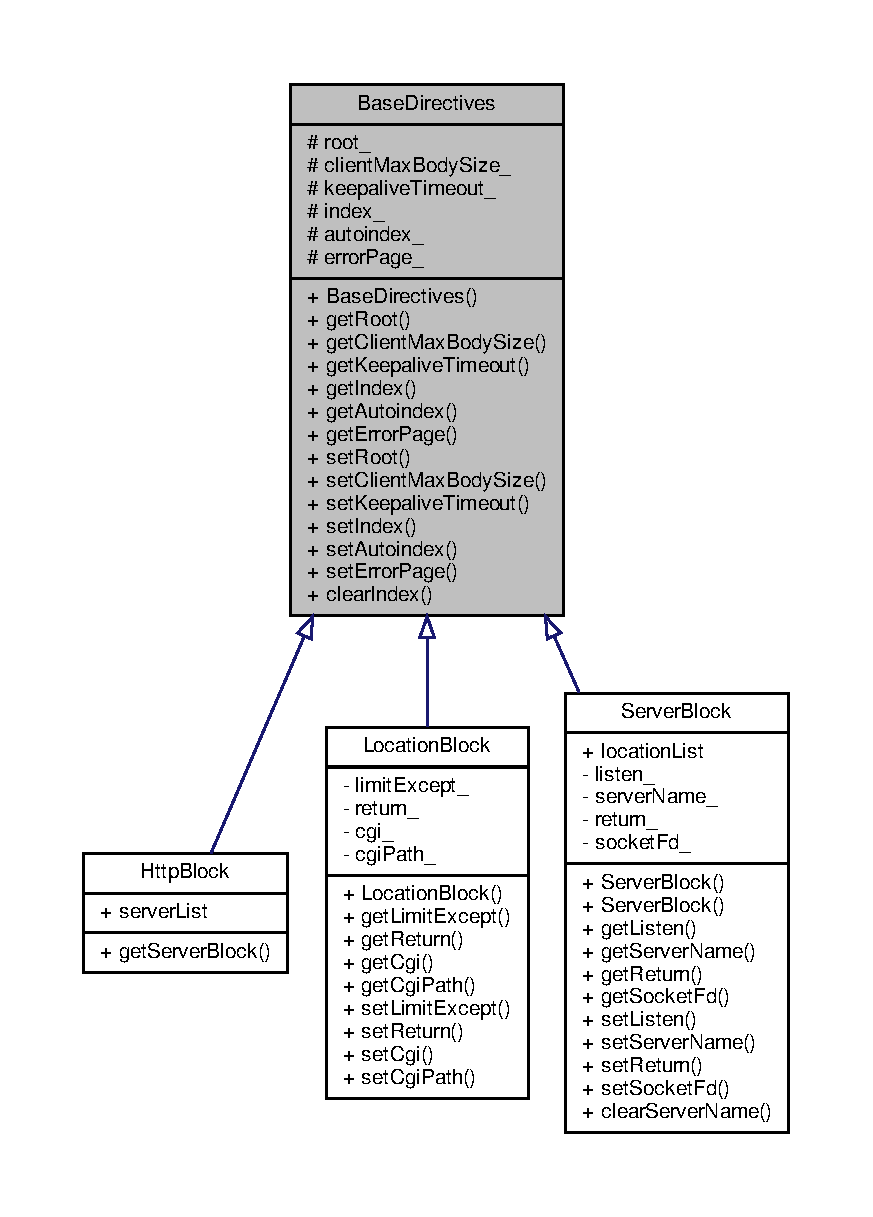
\includegraphics[width=350pt]{classft_1_1_base_directives__inherit__graph}
\end{center}
\end{figure}


Collaboration diagram for Base\+Directives\+:
\nopagebreak
\begin{figure}[H]
\begin{center}
\leavevmode
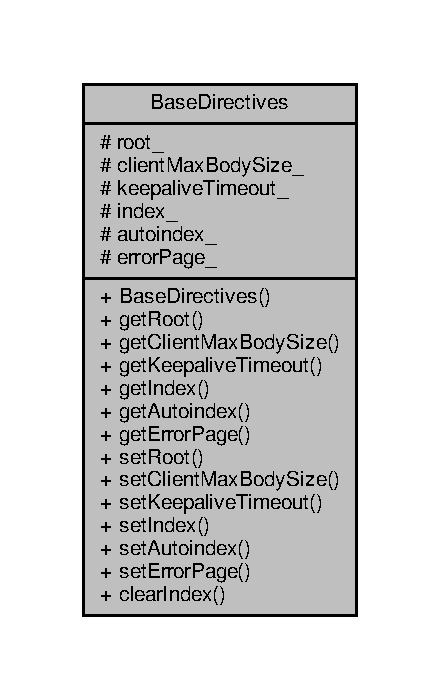
\includegraphics[width=211pt]{classft_1_1_base_directives__coll__graph}
\end{center}
\end{figure}
\subsection*{Public Member Functions}
\begin{DoxyCompactItemize}
\item 
\hyperlink{classft_1_1_base_directives_a2c932d87850535dd7655dc18f24740d9}{Base\+Directives} ()
\item 
const std\+::string \hyperlink{classft_1_1_base_directives_aa5dbcb08bda0a0e7e502d2df7cf64287}{get\+Root} (void) const
\item 
unsigned long \hyperlink{classft_1_1_base_directives_a930398ba1e4b99b2ba01a60dcda0c923}{get\+Client\+Max\+Body\+Size} (void) const
\item 
unsigned int \hyperlink{classft_1_1_base_directives_ab8574338758f65325cab5d1c394826c8}{get\+Keepalive\+Timeout} (void) const
\item 
const std\+::vector$<$ std\+::string $>$ \hyperlink{classft_1_1_base_directives_a018f34a5ffd66e891494b5c0ee69177b}{get\+Index} (void) const
\item 
bool \hyperlink{classft_1_1_base_directives_a4c11ed7ad76aeac228b029a2444de568}{get\+Autoindex} (void) const
\item 
const std\+::string \hyperlink{classft_1_1_base_directives_a3cb0c21f17781de392d5ee09d7190caf}{get\+Error\+Page} (void) const
\item 
void \hyperlink{classft_1_1_base_directives_a2a7990e309f7e38f2915dbbb0d2704cf}{set\+Root} (const std\+::string x)
\item 
void \hyperlink{classft_1_1_base_directives_a39bf4922f3236043c76beaffaa557a3b}{set\+Client\+Max\+Body\+Size} (const unsigned long x)
\item 
void \hyperlink{classft_1_1_base_directives_a0818b8529872ba9622329e2118d20c39}{set\+Keepalive\+Timeout} (const unsigned int x)
\item 
void \hyperlink{classft_1_1_base_directives_a6d3d8fd6eaaf71304128af6b3cee2a69}{set\+Index} (const std\+::string x)
\item 
void \hyperlink{classft_1_1_base_directives_ae7293c7bbf34e9bdc60c540dccd53342}{set\+Autoindex} (const bool x)
\item 
void \hyperlink{classft_1_1_base_directives_a505ecc88b3e1779583ad60cc243c7769}{set\+Error\+Page} (const std\+::string x)
\item 
void \hyperlink{classft_1_1_base_directives_a36d96dc74e650162c25a325813130ab2}{clear\+Index} (void)
\end{DoxyCompactItemize}
\subsection*{Protected Attributes}
\begin{DoxyCompactItemize}
\item 
std\+::string \hyperlink{classft_1_1_base_directives_abb1eaf0bba10b90172d6152e69457dc7}{root\+\_\+}
\item 
unsigned long \hyperlink{classft_1_1_base_directives_ad65c2594d2a90ca065d410dfd4066a19}{client\+Max\+Body\+Size\+\_\+}
\item 
unsigned int \hyperlink{classft_1_1_base_directives_aa1f5f394b428d0d18765a9b9e14e648f}{keepalive\+Timeout\+\_\+}
\item 
std\+::vector$<$ std\+::string $>$ \hyperlink{classft_1_1_base_directives_a6ba30626837f300201cd32c35d50aa49}{index\+\_\+}
\item 
bool \hyperlink{classft_1_1_base_directives_a4ebffbe32f50a462afa139c6f03c1a4f}{autoindex\+\_\+}
\item 
std\+::string \hyperlink{classft_1_1_base_directives_a5c0d388109f086503961de84fe3fce90}{error\+Page\+\_\+}
\end{DoxyCompactItemize}


\subsection{Detailed Description}


Definition at line 9 of file Base\+Directives.\+hpp.



\subsection{Constructor \& Destructor Documentation}
\mbox{\Hypertarget{classft_1_1_base_directives_a2c932d87850535dd7655dc18f24740d9}\label{classft_1_1_base_directives_a2c932d87850535dd7655dc18f24740d9}} 
\index{ft\+::\+Base\+Directives@{ft\+::\+Base\+Directives}!Base\+Directives@{Base\+Directives}}
\index{Base\+Directives@{Base\+Directives}!ft\+::\+Base\+Directives@{ft\+::\+Base\+Directives}}
\subsubsection{\texorpdfstring{Base\+Directives()}{BaseDirectives()}}
{\footnotesize\ttfamily \hyperlink{classft_1_1_base_directives}{Base\+Directives} (\begin{DoxyParamCaption}{ }\end{DoxyParamCaption})}



Definition at line 5 of file Base\+Directives.\+cpp.


\begin{DoxyCode}
6     \{
7         this->\hyperlink{classft_1_1_base_directives_abb1eaf0bba10b90172d6152e69457dc7}{root\_} = \textcolor{stringliteral}{"html"};
8         this->\hyperlink{classft_1_1_base_directives_ad65c2594d2a90ca065d410dfd4066a19}{clientMaxBodySize\_} = 1000000;
9         this->\hyperlink{classft_1_1_base_directives_aa1f5f394b428d0d18765a9b9e14e648f}{keepaliveTimeout\_} = 75;
10         this->\hyperlink{classft_1_1_base_directives_a6ba30626837f300201cd32c35d50aa49}{index\_}.push\_back(\textcolor{stringliteral}{"index.html"});
11         this->\hyperlink{classft_1_1_base_directives_a4ebffbe32f50a462afa139c6f03c1a4f}{autoindex\_} = \textcolor{stringliteral}{"off"};
12         this->\hyperlink{classft_1_1_base_directives_a5c0d388109f086503961de84fe3fce90}{errorPage\_} = \textcolor{stringliteral}{""};
13     \}
\end{DoxyCode}


\subsection{Member Function Documentation}
\mbox{\Hypertarget{classft_1_1_base_directives_a36d96dc74e650162c25a325813130ab2}\label{classft_1_1_base_directives_a36d96dc74e650162c25a325813130ab2}} 
\index{ft\+::\+Base\+Directives@{ft\+::\+Base\+Directives}!clear\+Index@{clear\+Index}}
\index{clear\+Index@{clear\+Index}!ft\+::\+Base\+Directives@{ft\+::\+Base\+Directives}}
\subsubsection{\texorpdfstring{clear\+Index()}{clearIndex()}}
{\footnotesize\ttfamily void clear\+Index (\begin{DoxyParamCaption}\item[{void}]{ }\end{DoxyParamCaption})}



Definition at line 78 of file Base\+Directives.\+cpp.


\begin{DoxyCode}
79     \{
80         this->\hyperlink{classft_1_1_base_directives_a6ba30626837f300201cd32c35d50aa49}{index\_}.clear();
81     \}
\end{DoxyCode}
Here is the caller graph for this function\+:
\nopagebreak
\begin{figure}[H]
\begin{center}
\leavevmode
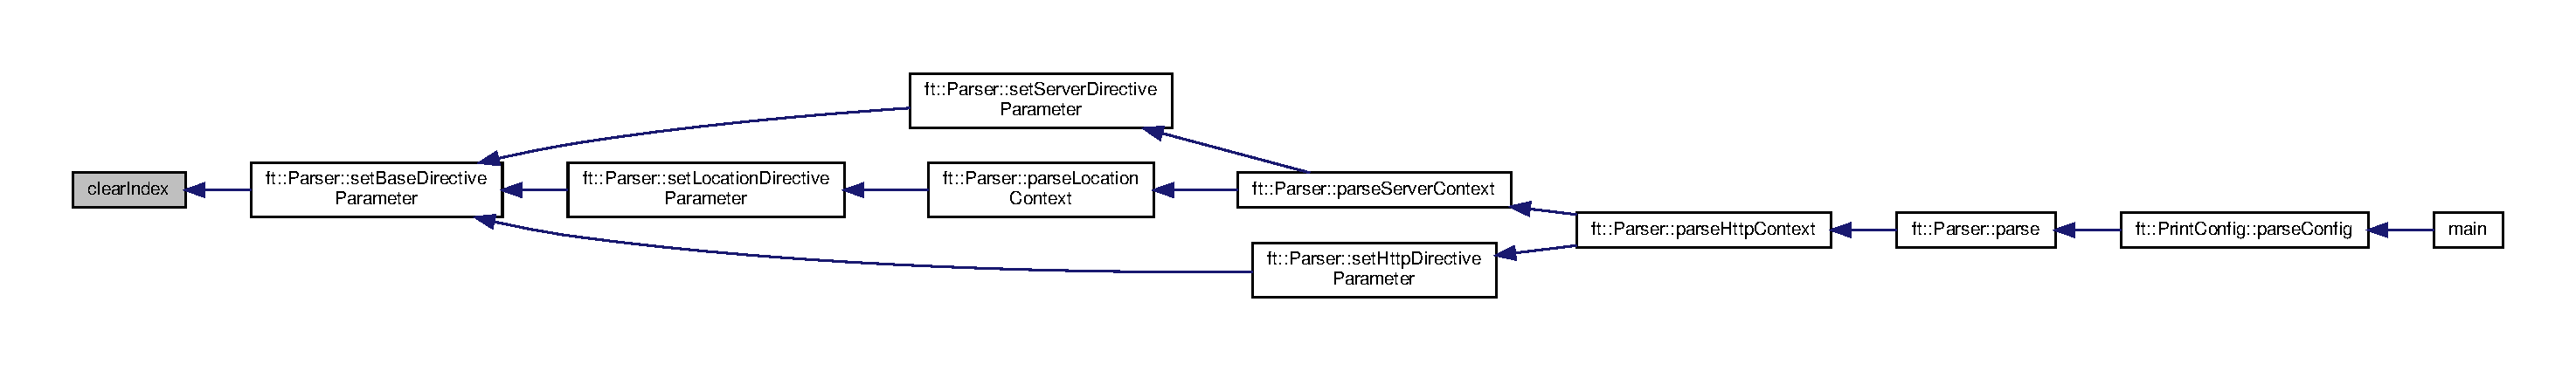
\includegraphics[width=350pt]{classft_1_1_base_directives_a36d96dc74e650162c25a325813130ab2_icgraph}
\end{center}
\end{figure}
\mbox{\Hypertarget{classft_1_1_base_directives_a4c11ed7ad76aeac228b029a2444de568}\label{classft_1_1_base_directives_a4c11ed7ad76aeac228b029a2444de568}} 
\index{ft\+::\+Base\+Directives@{ft\+::\+Base\+Directives}!get\+Autoindex@{get\+Autoindex}}
\index{get\+Autoindex@{get\+Autoindex}!ft\+::\+Base\+Directives@{ft\+::\+Base\+Directives}}
\subsubsection{\texorpdfstring{get\+Autoindex()}{getAutoindex()}}
{\footnotesize\ttfamily bool get\+Autoindex (\begin{DoxyParamCaption}\item[{void}]{ }\end{DoxyParamCaption}) const}



Definition at line 36 of file Base\+Directives.\+cpp.


\begin{DoxyCode}
37     \{
38         \textcolor{keywordflow}{return} (this->\hyperlink{classft_1_1_base_directives_a4ebffbe32f50a462afa139c6f03c1a4f}{autoindex\_});
39     \}
\end{DoxyCode}
Here is the caller graph for this function\+:
\nopagebreak
\begin{figure}[H]
\begin{center}
\leavevmode
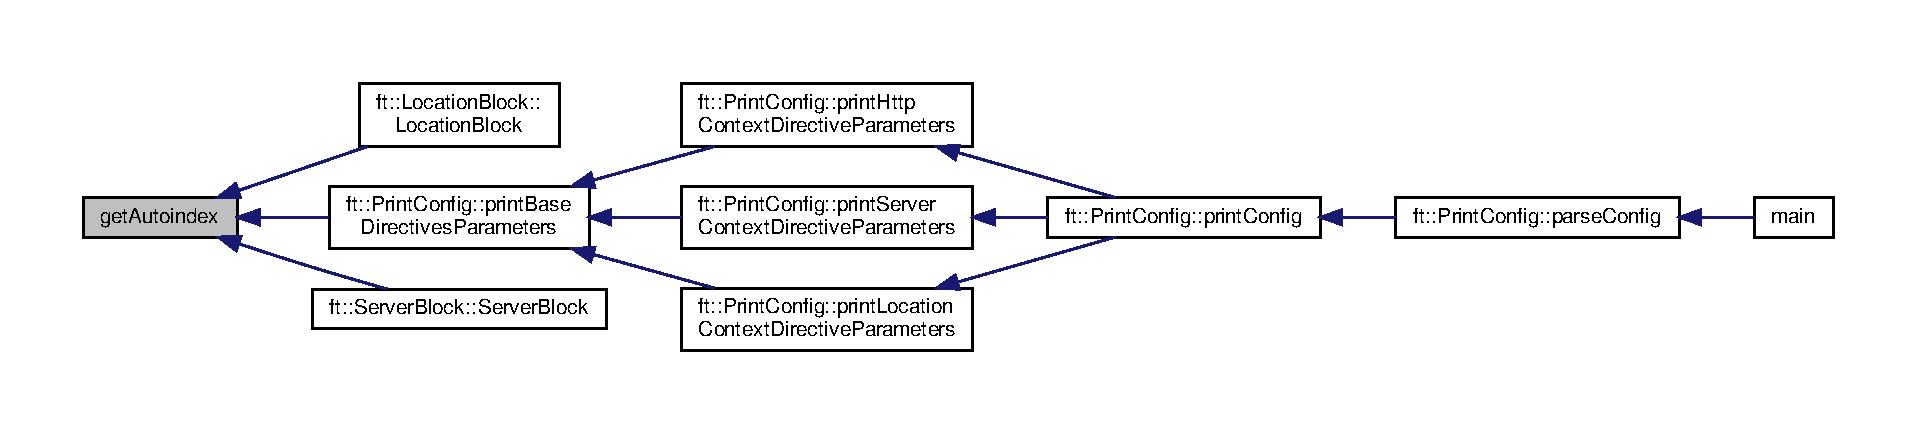
\includegraphics[width=350pt]{classft_1_1_base_directives_a4c11ed7ad76aeac228b029a2444de568_icgraph}
\end{center}
\end{figure}
\mbox{\Hypertarget{classft_1_1_base_directives_a930398ba1e4b99b2ba01a60dcda0c923}\label{classft_1_1_base_directives_a930398ba1e4b99b2ba01a60dcda0c923}} 
\index{ft\+::\+Base\+Directives@{ft\+::\+Base\+Directives}!get\+Client\+Max\+Body\+Size@{get\+Client\+Max\+Body\+Size}}
\index{get\+Client\+Max\+Body\+Size@{get\+Client\+Max\+Body\+Size}!ft\+::\+Base\+Directives@{ft\+::\+Base\+Directives}}
\subsubsection{\texorpdfstring{get\+Client\+Max\+Body\+Size()}{getClientMaxBodySize()}}
{\footnotesize\ttfamily unsigned long get\+Client\+Max\+Body\+Size (\begin{DoxyParamCaption}\item[{void}]{ }\end{DoxyParamCaption}) const}



Definition at line 21 of file Base\+Directives.\+cpp.


\begin{DoxyCode}
22     \{
23         \textcolor{keywordflow}{return} (this->\hyperlink{classft_1_1_base_directives_ad65c2594d2a90ca065d410dfd4066a19}{clientMaxBodySize\_});
24     \}
\end{DoxyCode}
Here is the caller graph for this function\+:
\nopagebreak
\begin{figure}[H]
\begin{center}
\leavevmode
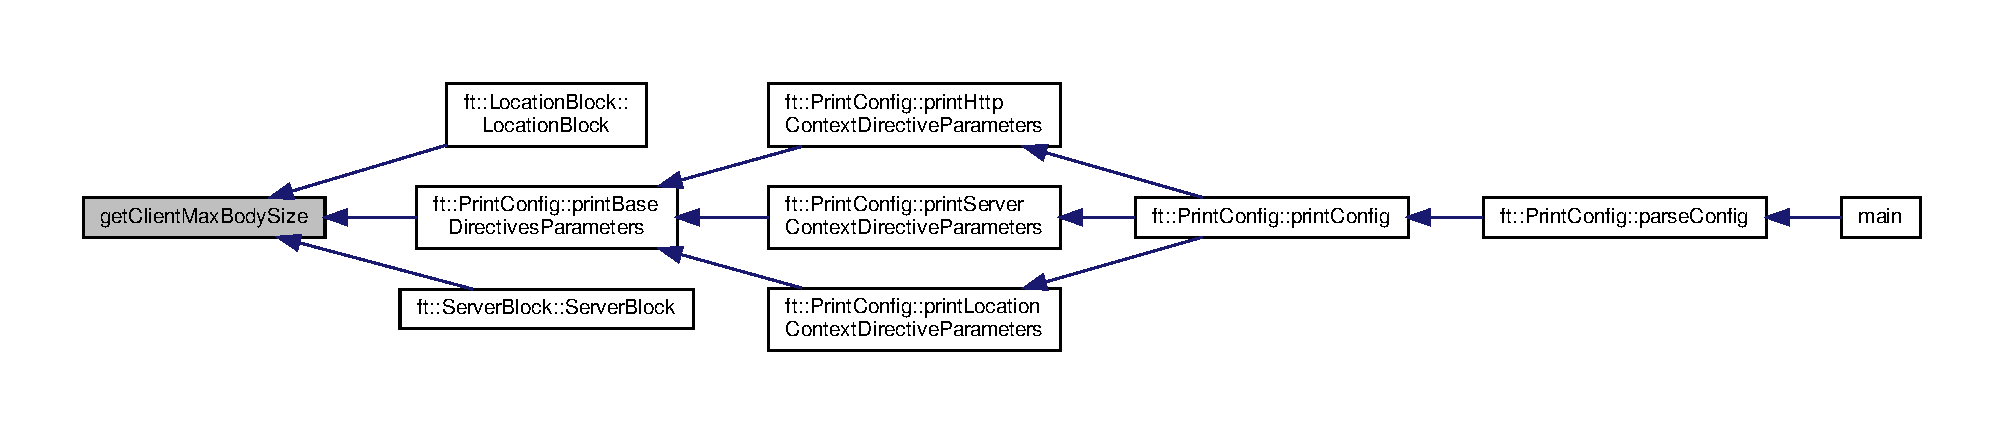
\includegraphics[width=350pt]{classft_1_1_base_directives_a930398ba1e4b99b2ba01a60dcda0c923_icgraph}
\end{center}
\end{figure}
\mbox{\Hypertarget{classft_1_1_base_directives_a3cb0c21f17781de392d5ee09d7190caf}\label{classft_1_1_base_directives_a3cb0c21f17781de392d5ee09d7190caf}} 
\index{ft\+::\+Base\+Directives@{ft\+::\+Base\+Directives}!get\+Error\+Page@{get\+Error\+Page}}
\index{get\+Error\+Page@{get\+Error\+Page}!ft\+::\+Base\+Directives@{ft\+::\+Base\+Directives}}
\subsubsection{\texorpdfstring{get\+Error\+Page()}{getErrorPage()}}
{\footnotesize\ttfamily const std\+::string get\+Error\+Page (\begin{DoxyParamCaption}\item[{void}]{ }\end{DoxyParamCaption}) const}



Definition at line 41 of file Base\+Directives.\+cpp.


\begin{DoxyCode}
42     \{
43         \textcolor{keywordflow}{return} (this->\hyperlink{classft_1_1_base_directives_a5c0d388109f086503961de84fe3fce90}{errorPage\_});
44     \}
\end{DoxyCode}
Here is the caller graph for this function\+:
\nopagebreak
\begin{figure}[H]
\begin{center}
\leavevmode
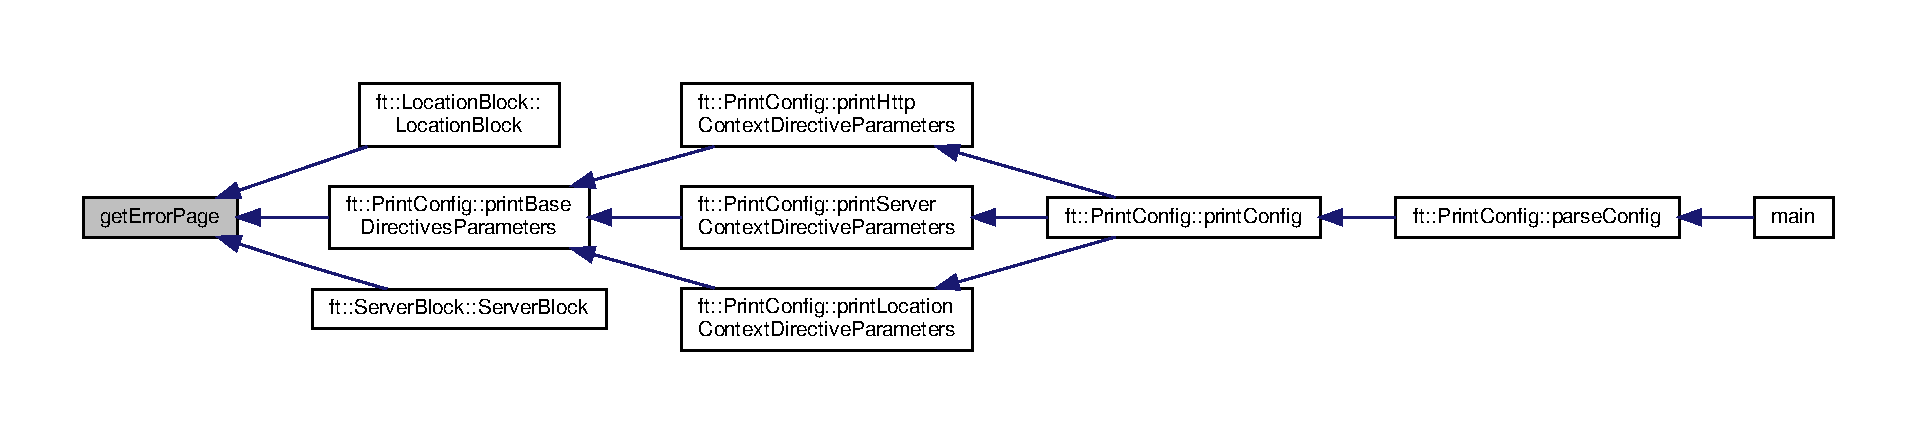
\includegraphics[width=350pt]{classft_1_1_base_directives_a3cb0c21f17781de392d5ee09d7190caf_icgraph}
\end{center}
\end{figure}
\mbox{\Hypertarget{classft_1_1_base_directives_a018f34a5ffd66e891494b5c0ee69177b}\label{classft_1_1_base_directives_a018f34a5ffd66e891494b5c0ee69177b}} 
\index{ft\+::\+Base\+Directives@{ft\+::\+Base\+Directives}!get\+Index@{get\+Index}}
\index{get\+Index@{get\+Index}!ft\+::\+Base\+Directives@{ft\+::\+Base\+Directives}}
\subsubsection{\texorpdfstring{get\+Index()}{getIndex()}}
{\footnotesize\ttfamily const std\+::vector$<$ std\+::string $>$ get\+Index (\begin{DoxyParamCaption}\item[{void}]{ }\end{DoxyParamCaption}) const}



Definition at line 31 of file Base\+Directives.\+cpp.


\begin{DoxyCode}
32     \{
33         \textcolor{keywordflow}{return} (this->\hyperlink{classft_1_1_base_directives_a6ba30626837f300201cd32c35d50aa49}{index\_});
34     \}
\end{DoxyCode}
Here is the caller graph for this function\+:
\nopagebreak
\begin{figure}[H]
\begin{center}
\leavevmode
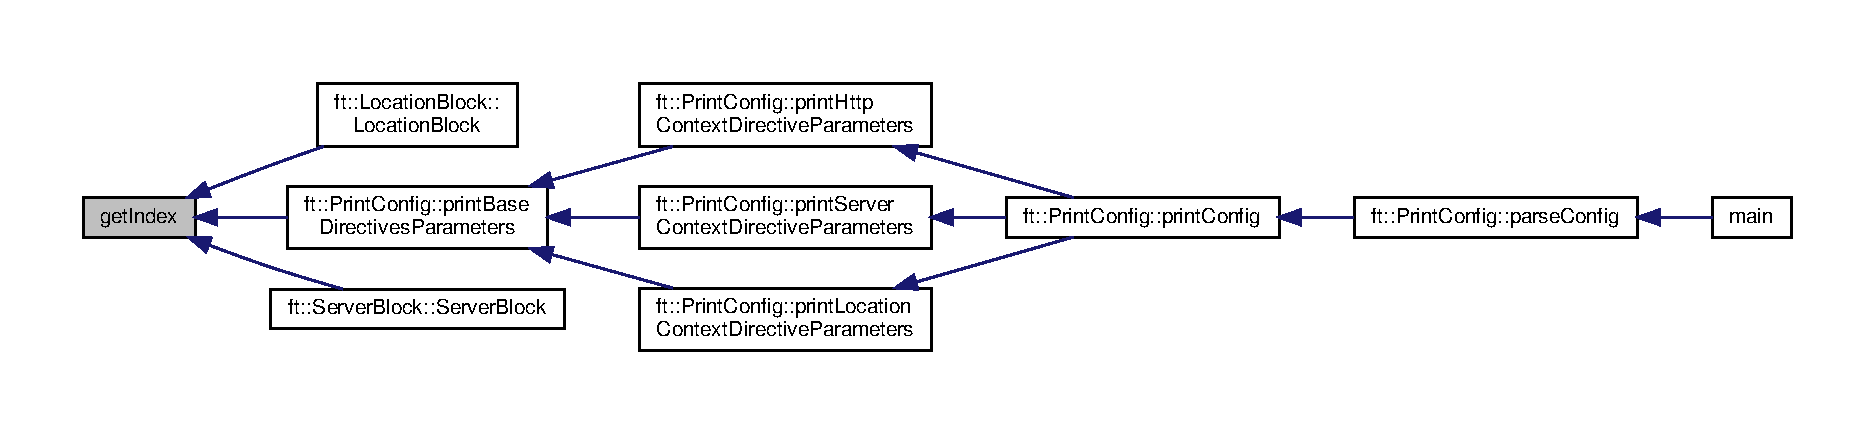
\includegraphics[width=350pt]{classft_1_1_base_directives_a018f34a5ffd66e891494b5c0ee69177b_icgraph}
\end{center}
\end{figure}
\mbox{\Hypertarget{classft_1_1_base_directives_ab8574338758f65325cab5d1c394826c8}\label{classft_1_1_base_directives_ab8574338758f65325cab5d1c394826c8}} 
\index{ft\+::\+Base\+Directives@{ft\+::\+Base\+Directives}!get\+Keepalive\+Timeout@{get\+Keepalive\+Timeout}}
\index{get\+Keepalive\+Timeout@{get\+Keepalive\+Timeout}!ft\+::\+Base\+Directives@{ft\+::\+Base\+Directives}}
\subsubsection{\texorpdfstring{get\+Keepalive\+Timeout()}{getKeepaliveTimeout()}}
{\footnotesize\ttfamily unsigned int get\+Keepalive\+Timeout (\begin{DoxyParamCaption}\item[{void}]{ }\end{DoxyParamCaption}) const}



Definition at line 26 of file Base\+Directives.\+cpp.


\begin{DoxyCode}
27     \{
28         \textcolor{keywordflow}{return} (this->\hyperlink{classft_1_1_base_directives_aa1f5f394b428d0d18765a9b9e14e648f}{keepaliveTimeout\_});
29     \}
\end{DoxyCode}
Here is the caller graph for this function\+:
\nopagebreak
\begin{figure}[H]
\begin{center}
\leavevmode
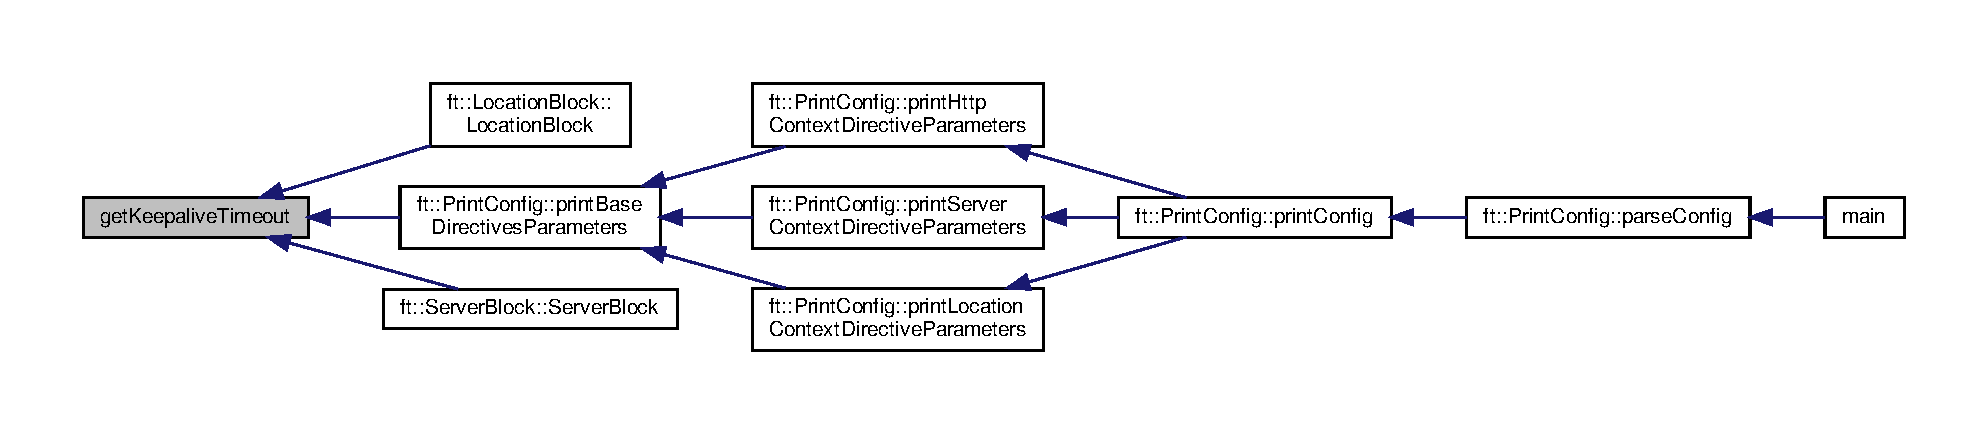
\includegraphics[width=350pt]{classft_1_1_base_directives_ab8574338758f65325cab5d1c394826c8_icgraph}
\end{center}
\end{figure}
\mbox{\Hypertarget{classft_1_1_base_directives_aa5dbcb08bda0a0e7e502d2df7cf64287}\label{classft_1_1_base_directives_aa5dbcb08bda0a0e7e502d2df7cf64287}} 
\index{ft\+::\+Base\+Directives@{ft\+::\+Base\+Directives}!get\+Root@{get\+Root}}
\index{get\+Root@{get\+Root}!ft\+::\+Base\+Directives@{ft\+::\+Base\+Directives}}
\subsubsection{\texorpdfstring{get\+Root()}{getRoot()}}
{\footnotesize\ttfamily const std\+::string get\+Root (\begin{DoxyParamCaption}\item[{void}]{ }\end{DoxyParamCaption}) const}



Definition at line 16 of file Base\+Directives.\+cpp.


\begin{DoxyCode}
17     \{
18         \textcolor{keywordflow}{return} (this->\hyperlink{classft_1_1_base_directives_abb1eaf0bba10b90172d6152e69457dc7}{root\_});
19     \}
\end{DoxyCode}
Here is the caller graph for this function\+:
\nopagebreak
\begin{figure}[H]
\begin{center}
\leavevmode
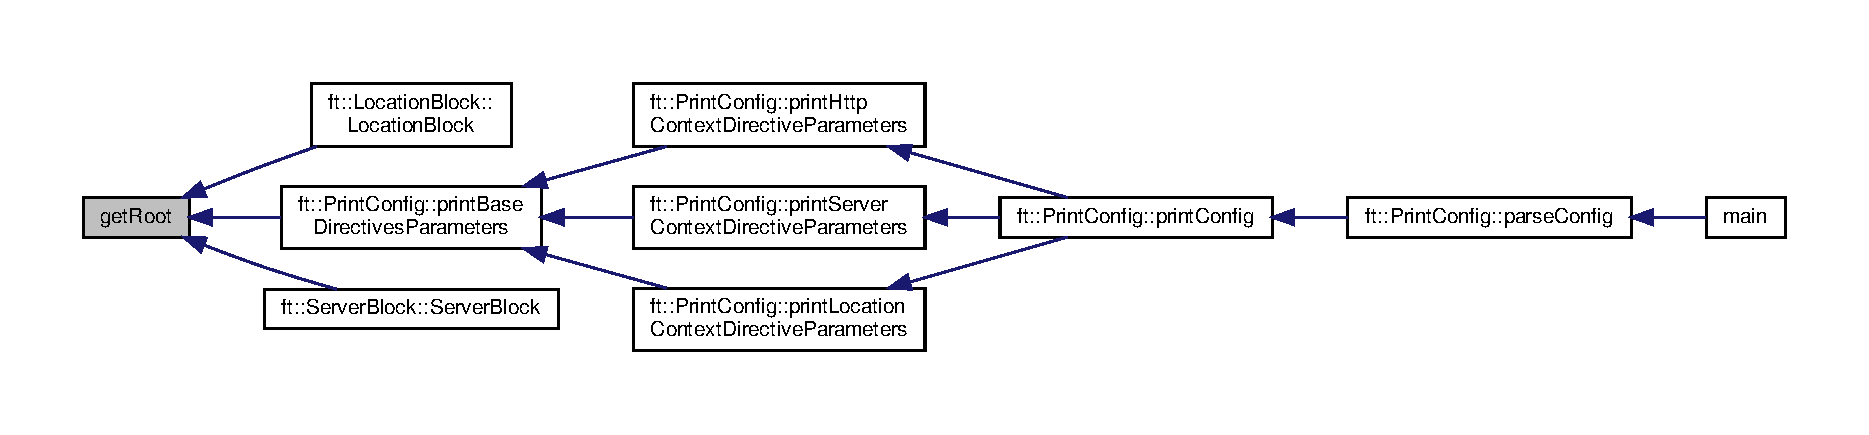
\includegraphics[width=350pt]{classft_1_1_base_directives_aa5dbcb08bda0a0e7e502d2df7cf64287_icgraph}
\end{center}
\end{figure}
\mbox{\Hypertarget{classft_1_1_base_directives_ae7293c7bbf34e9bdc60c540dccd53342}\label{classft_1_1_base_directives_ae7293c7bbf34e9bdc60c540dccd53342}} 
\index{ft\+::\+Base\+Directives@{ft\+::\+Base\+Directives}!set\+Autoindex@{set\+Autoindex}}
\index{set\+Autoindex@{set\+Autoindex}!ft\+::\+Base\+Directives@{ft\+::\+Base\+Directives}}
\subsubsection{\texorpdfstring{set\+Autoindex()}{setAutoindex()}}
{\footnotesize\ttfamily void set\+Autoindex (\begin{DoxyParamCaption}\item[{const bool}]{x }\end{DoxyParamCaption})}



Definition at line 67 of file Base\+Directives.\+cpp.


\begin{DoxyCode}
68     \{
69         this->\hyperlink{classft_1_1_base_directives_a4ebffbe32f50a462afa139c6f03c1a4f}{autoindex\_} = x;
70     \}
\end{DoxyCode}
Here is the caller graph for this function\+:
\nopagebreak
\begin{figure}[H]
\begin{center}
\leavevmode
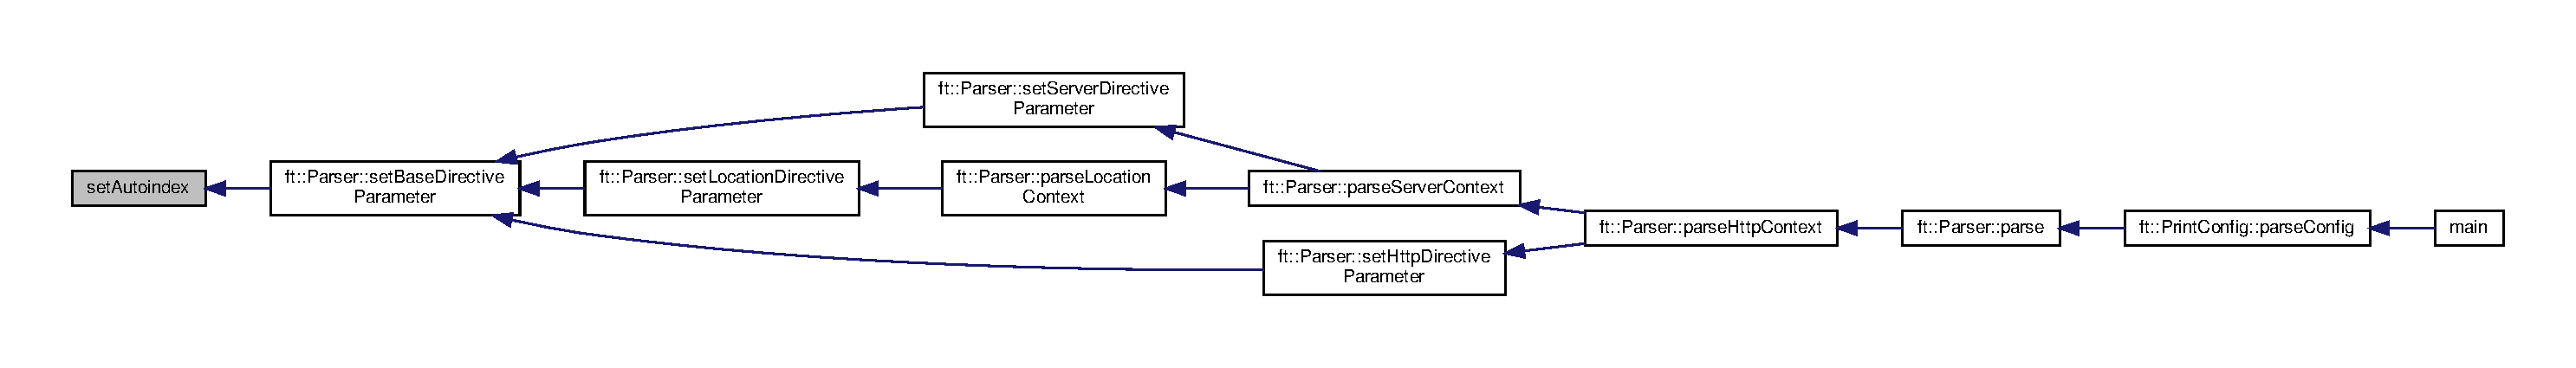
\includegraphics[width=350pt]{classft_1_1_base_directives_ae7293c7bbf34e9bdc60c540dccd53342_icgraph}
\end{center}
\end{figure}
\mbox{\Hypertarget{classft_1_1_base_directives_a39bf4922f3236043c76beaffaa557a3b}\label{classft_1_1_base_directives_a39bf4922f3236043c76beaffaa557a3b}} 
\index{ft\+::\+Base\+Directives@{ft\+::\+Base\+Directives}!set\+Client\+Max\+Body\+Size@{set\+Client\+Max\+Body\+Size}}
\index{set\+Client\+Max\+Body\+Size@{set\+Client\+Max\+Body\+Size}!ft\+::\+Base\+Directives@{ft\+::\+Base\+Directives}}
\subsubsection{\texorpdfstring{set\+Client\+Max\+Body\+Size()}{setClientMaxBodySize()}}
{\footnotesize\ttfamily void set\+Client\+Max\+Body\+Size (\begin{DoxyParamCaption}\item[{const unsigned long}]{x }\end{DoxyParamCaption})}



Definition at line 52 of file Base\+Directives.\+cpp.


\begin{DoxyCode}
53     \{
54         this->\hyperlink{classft_1_1_base_directives_ad65c2594d2a90ca065d410dfd4066a19}{clientMaxBodySize\_} = x;
55     \}
\end{DoxyCode}
Here is the caller graph for this function\+:
\nopagebreak
\begin{figure}[H]
\begin{center}
\leavevmode
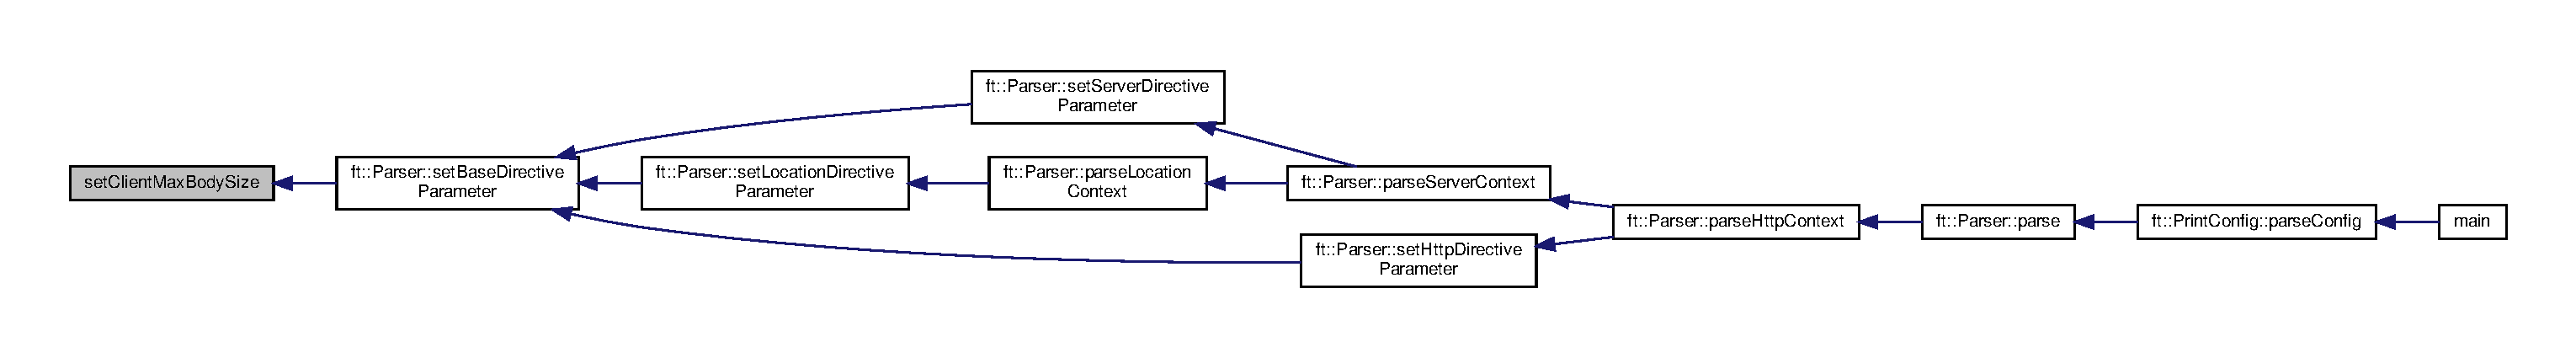
\includegraphics[width=350pt]{classft_1_1_base_directives_a39bf4922f3236043c76beaffaa557a3b_icgraph}
\end{center}
\end{figure}
\mbox{\Hypertarget{classft_1_1_base_directives_a505ecc88b3e1779583ad60cc243c7769}\label{classft_1_1_base_directives_a505ecc88b3e1779583ad60cc243c7769}} 
\index{ft\+::\+Base\+Directives@{ft\+::\+Base\+Directives}!set\+Error\+Page@{set\+Error\+Page}}
\index{set\+Error\+Page@{set\+Error\+Page}!ft\+::\+Base\+Directives@{ft\+::\+Base\+Directives}}
\subsubsection{\texorpdfstring{set\+Error\+Page()}{setErrorPage()}}
{\footnotesize\ttfamily void set\+Error\+Page (\begin{DoxyParamCaption}\item[{const std\+::string}]{x }\end{DoxyParamCaption})}



Definition at line 72 of file Base\+Directives.\+cpp.


\begin{DoxyCode}
73     \{
74         this->\hyperlink{classft_1_1_base_directives_a5c0d388109f086503961de84fe3fce90}{errorPage\_} = x;
75     \}
\end{DoxyCode}
Here is the caller graph for this function\+:
\nopagebreak
\begin{figure}[H]
\begin{center}
\leavevmode
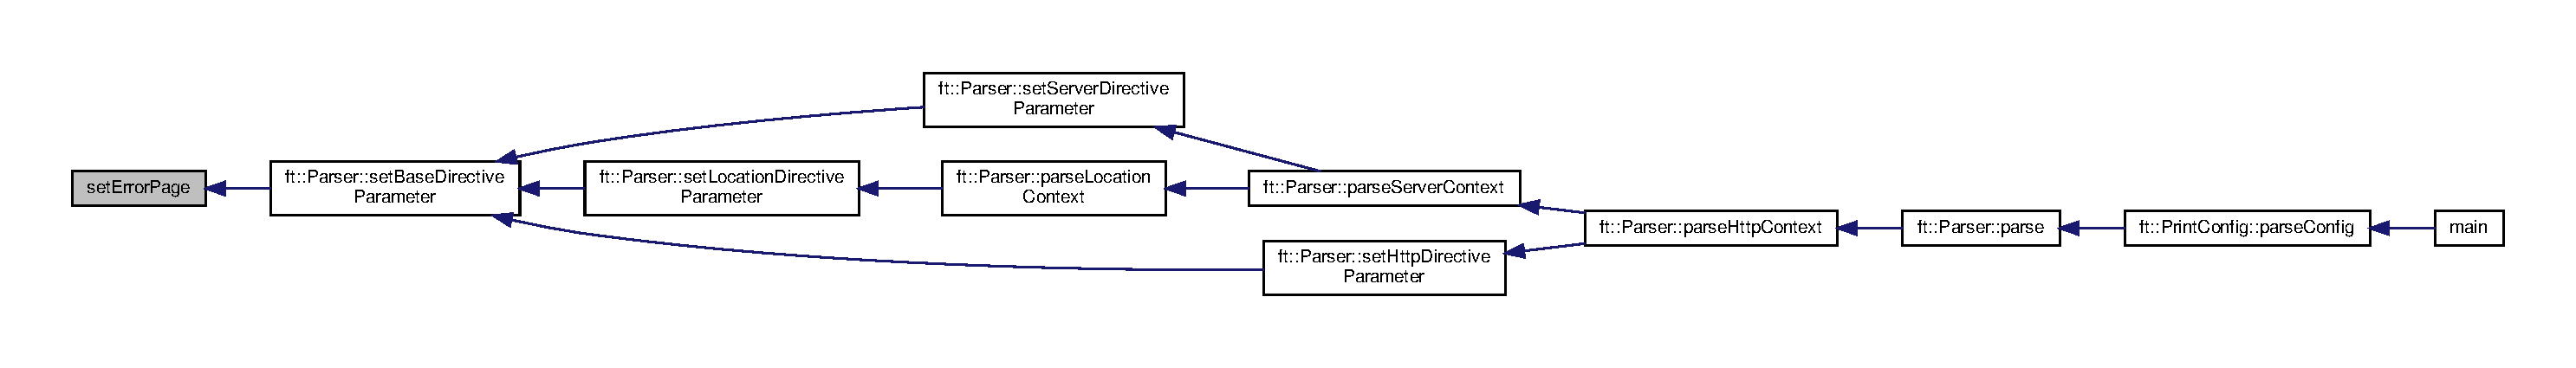
\includegraphics[width=350pt]{classft_1_1_base_directives_a505ecc88b3e1779583ad60cc243c7769_icgraph}
\end{center}
\end{figure}
\mbox{\Hypertarget{classft_1_1_base_directives_a6d3d8fd6eaaf71304128af6b3cee2a69}\label{classft_1_1_base_directives_a6d3d8fd6eaaf71304128af6b3cee2a69}} 
\index{ft\+::\+Base\+Directives@{ft\+::\+Base\+Directives}!set\+Index@{set\+Index}}
\index{set\+Index@{set\+Index}!ft\+::\+Base\+Directives@{ft\+::\+Base\+Directives}}
\subsubsection{\texorpdfstring{set\+Index()}{setIndex()}}
{\footnotesize\ttfamily void set\+Index (\begin{DoxyParamCaption}\item[{const std\+::string}]{x }\end{DoxyParamCaption})}



Definition at line 62 of file Base\+Directives.\+cpp.


\begin{DoxyCode}
63     \{
64         this->\hyperlink{classft_1_1_base_directives_a6ba30626837f300201cd32c35d50aa49}{index\_}.push\_back(x);
65     \}
\end{DoxyCode}
Here is the caller graph for this function\+:
\nopagebreak
\begin{figure}[H]
\begin{center}
\leavevmode
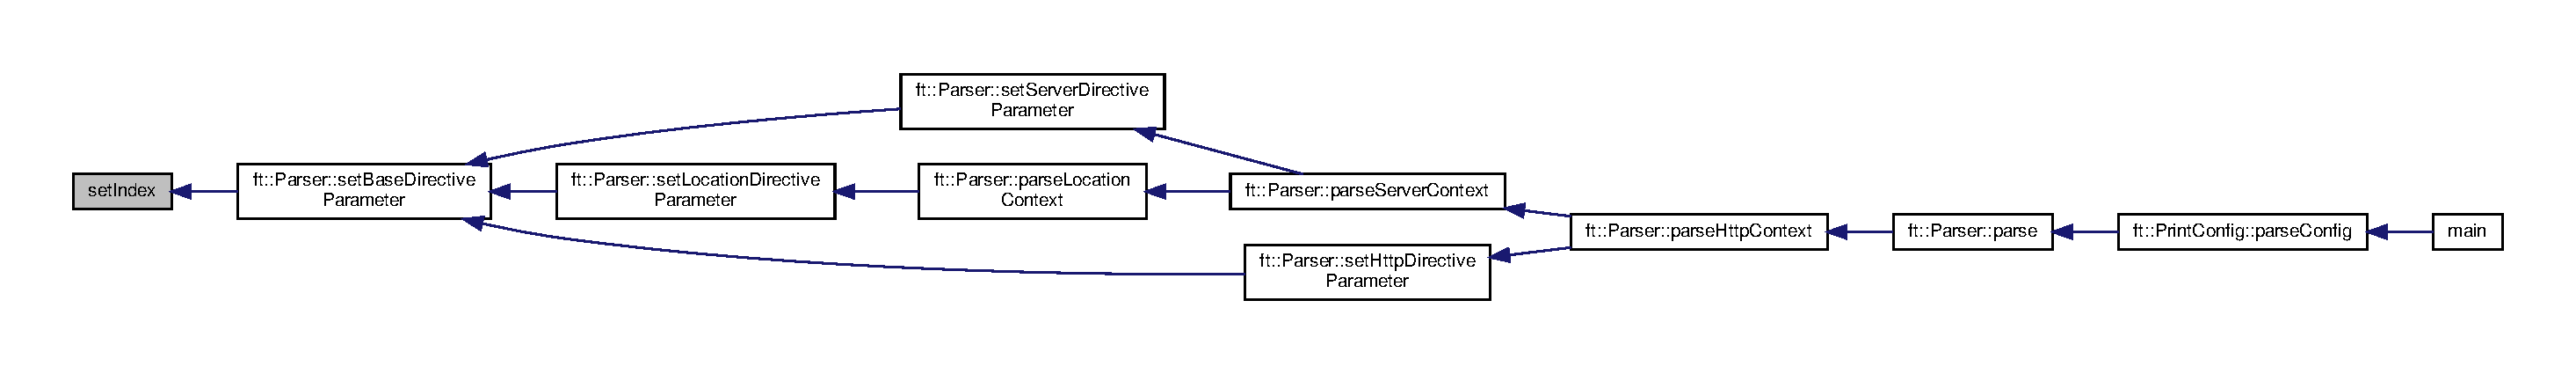
\includegraphics[width=350pt]{classft_1_1_base_directives_a6d3d8fd6eaaf71304128af6b3cee2a69_icgraph}
\end{center}
\end{figure}
\mbox{\Hypertarget{classft_1_1_base_directives_a0818b8529872ba9622329e2118d20c39}\label{classft_1_1_base_directives_a0818b8529872ba9622329e2118d20c39}} 
\index{ft\+::\+Base\+Directives@{ft\+::\+Base\+Directives}!set\+Keepalive\+Timeout@{set\+Keepalive\+Timeout}}
\index{set\+Keepalive\+Timeout@{set\+Keepalive\+Timeout}!ft\+::\+Base\+Directives@{ft\+::\+Base\+Directives}}
\subsubsection{\texorpdfstring{set\+Keepalive\+Timeout()}{setKeepaliveTimeout()}}
{\footnotesize\ttfamily void set\+Keepalive\+Timeout (\begin{DoxyParamCaption}\item[{const unsigned int}]{x }\end{DoxyParamCaption})}



Definition at line 57 of file Base\+Directives.\+cpp.


\begin{DoxyCode}
58     \{
59         this->\hyperlink{classft_1_1_base_directives_aa1f5f394b428d0d18765a9b9e14e648f}{keepaliveTimeout\_} = x;
60     \}
\end{DoxyCode}
Here is the caller graph for this function\+:
\nopagebreak
\begin{figure}[H]
\begin{center}
\leavevmode
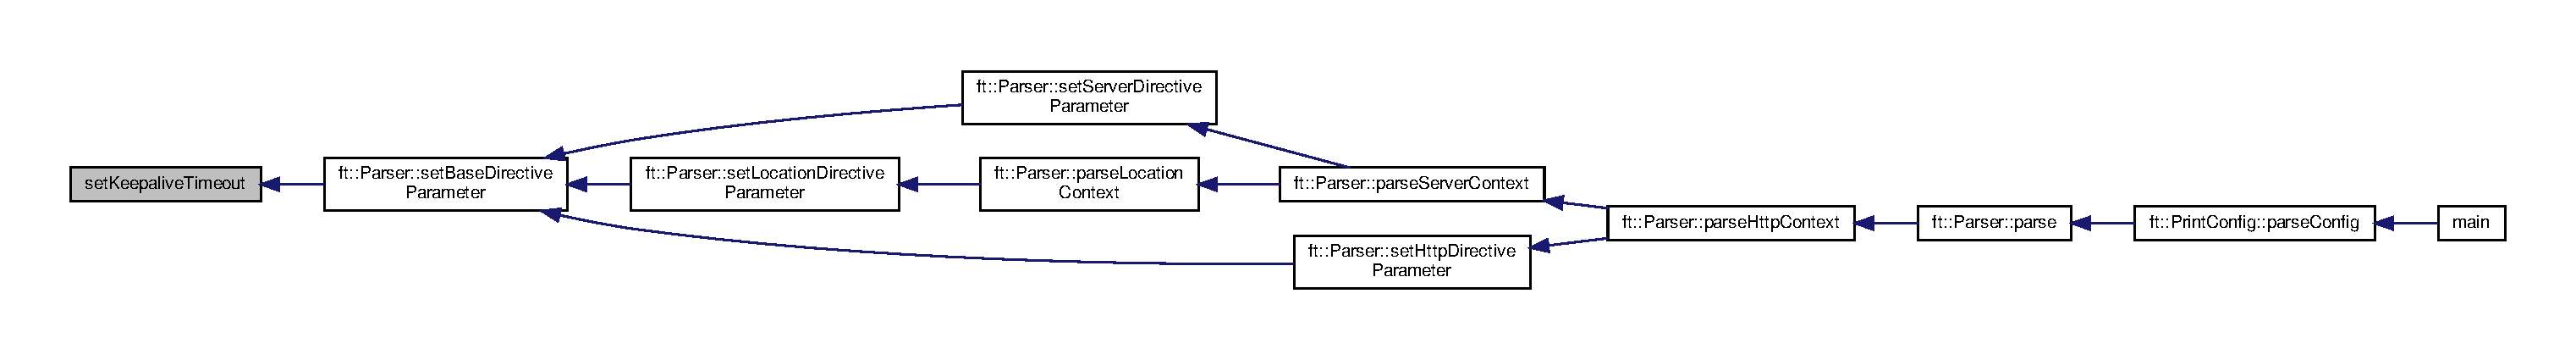
\includegraphics[width=350pt]{classft_1_1_base_directives_a0818b8529872ba9622329e2118d20c39_icgraph}
\end{center}
\end{figure}
\mbox{\Hypertarget{classft_1_1_base_directives_a2a7990e309f7e38f2915dbbb0d2704cf}\label{classft_1_1_base_directives_a2a7990e309f7e38f2915dbbb0d2704cf}} 
\index{ft\+::\+Base\+Directives@{ft\+::\+Base\+Directives}!set\+Root@{set\+Root}}
\index{set\+Root@{set\+Root}!ft\+::\+Base\+Directives@{ft\+::\+Base\+Directives}}
\subsubsection{\texorpdfstring{set\+Root()}{setRoot()}}
{\footnotesize\ttfamily void set\+Root (\begin{DoxyParamCaption}\item[{const std\+::string}]{x }\end{DoxyParamCaption})}



Definition at line 47 of file Base\+Directives.\+cpp.


\begin{DoxyCode}
48     \{
49         this->\hyperlink{classft_1_1_base_directives_abb1eaf0bba10b90172d6152e69457dc7}{root\_} = x;
50     \}
\end{DoxyCode}
Here is the caller graph for this function\+:
\nopagebreak
\begin{figure}[H]
\begin{center}
\leavevmode
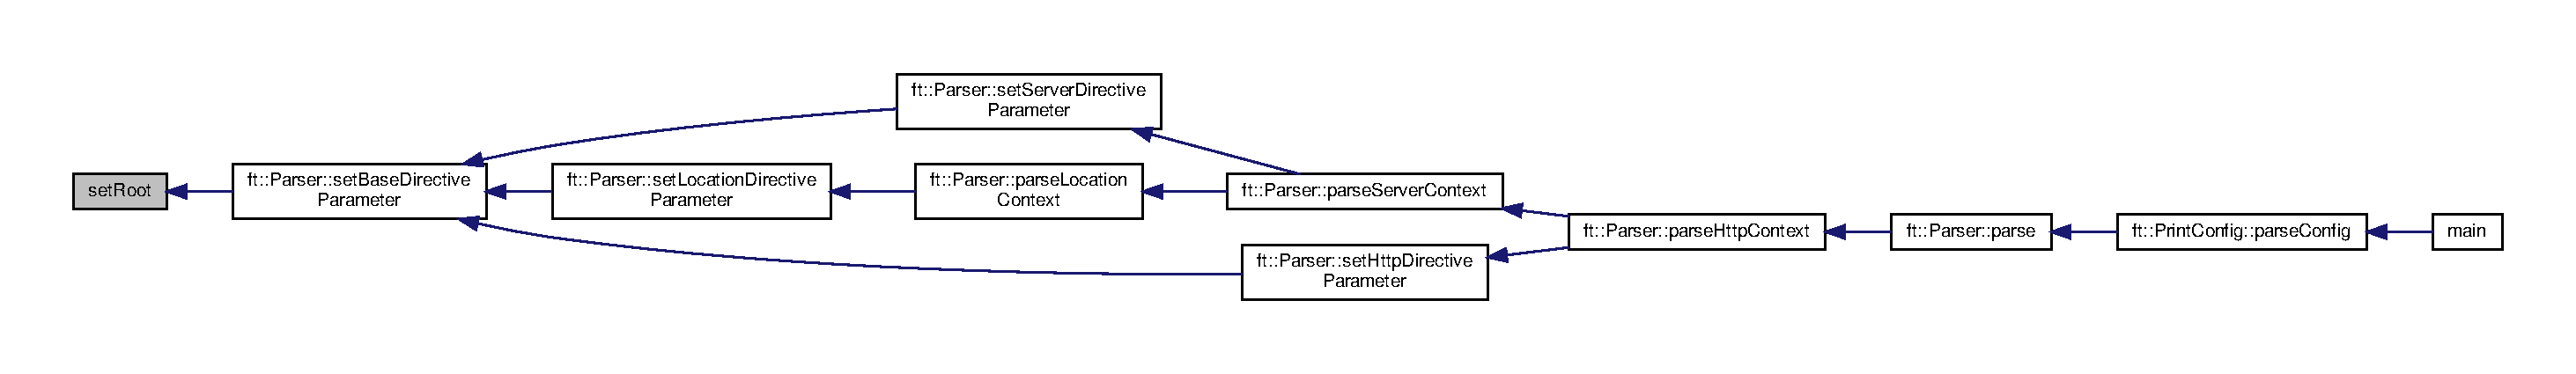
\includegraphics[width=350pt]{classft_1_1_base_directives_a2a7990e309f7e38f2915dbbb0d2704cf_icgraph}
\end{center}
\end{figure}


\subsection{Member Data Documentation}
\mbox{\Hypertarget{classft_1_1_base_directives_a4ebffbe32f50a462afa139c6f03c1a4f}\label{classft_1_1_base_directives_a4ebffbe32f50a462afa139c6f03c1a4f}} 
\index{ft\+::\+Base\+Directives@{ft\+::\+Base\+Directives}!autoindex\+\_\+@{autoindex\+\_\+}}
\index{autoindex\+\_\+@{autoindex\+\_\+}!ft\+::\+Base\+Directives@{ft\+::\+Base\+Directives}}
\subsubsection{\texorpdfstring{autoindex\+\_\+}{autoindex\_}}
{\footnotesize\ttfamily bool autoindex\+\_\+\hspace{0.3cm}{\ttfamily [protected]}}



Definition at line 16 of file Base\+Directives.\+hpp.

\mbox{\Hypertarget{classft_1_1_base_directives_ad65c2594d2a90ca065d410dfd4066a19}\label{classft_1_1_base_directives_ad65c2594d2a90ca065d410dfd4066a19}} 
\index{ft\+::\+Base\+Directives@{ft\+::\+Base\+Directives}!client\+Max\+Body\+Size\+\_\+@{client\+Max\+Body\+Size\+\_\+}}
\index{client\+Max\+Body\+Size\+\_\+@{client\+Max\+Body\+Size\+\_\+}!ft\+::\+Base\+Directives@{ft\+::\+Base\+Directives}}
\subsubsection{\texorpdfstring{client\+Max\+Body\+Size\+\_\+}{clientMaxBodySize\_}}
{\footnotesize\ttfamily unsigned long client\+Max\+Body\+Size\+\_\+\hspace{0.3cm}{\ttfamily [protected]}}



Definition at line 13 of file Base\+Directives.\+hpp.

\mbox{\Hypertarget{classft_1_1_base_directives_a5c0d388109f086503961de84fe3fce90}\label{classft_1_1_base_directives_a5c0d388109f086503961de84fe3fce90}} 
\index{ft\+::\+Base\+Directives@{ft\+::\+Base\+Directives}!error\+Page\+\_\+@{error\+Page\+\_\+}}
\index{error\+Page\+\_\+@{error\+Page\+\_\+}!ft\+::\+Base\+Directives@{ft\+::\+Base\+Directives}}
\subsubsection{\texorpdfstring{error\+Page\+\_\+}{errorPage\_}}
{\footnotesize\ttfamily std\+::string error\+Page\+\_\+\hspace{0.3cm}{\ttfamily [protected]}}



Definition at line 17 of file Base\+Directives.\+hpp.

\mbox{\Hypertarget{classft_1_1_base_directives_a6ba30626837f300201cd32c35d50aa49}\label{classft_1_1_base_directives_a6ba30626837f300201cd32c35d50aa49}} 
\index{ft\+::\+Base\+Directives@{ft\+::\+Base\+Directives}!index\+\_\+@{index\+\_\+}}
\index{index\+\_\+@{index\+\_\+}!ft\+::\+Base\+Directives@{ft\+::\+Base\+Directives}}
\subsubsection{\texorpdfstring{index\+\_\+}{index\_}}
{\footnotesize\ttfamily std\+::vector$<$std\+::string$>$ index\+\_\+\hspace{0.3cm}{\ttfamily [protected]}}



Definition at line 15 of file Base\+Directives.\+hpp.

\mbox{\Hypertarget{classft_1_1_base_directives_aa1f5f394b428d0d18765a9b9e14e648f}\label{classft_1_1_base_directives_aa1f5f394b428d0d18765a9b9e14e648f}} 
\index{ft\+::\+Base\+Directives@{ft\+::\+Base\+Directives}!keepalive\+Timeout\+\_\+@{keepalive\+Timeout\+\_\+}}
\index{keepalive\+Timeout\+\_\+@{keepalive\+Timeout\+\_\+}!ft\+::\+Base\+Directives@{ft\+::\+Base\+Directives}}
\subsubsection{\texorpdfstring{keepalive\+Timeout\+\_\+}{keepaliveTimeout\_}}
{\footnotesize\ttfamily unsigned int keepalive\+Timeout\+\_\+\hspace{0.3cm}{\ttfamily [protected]}}



Definition at line 14 of file Base\+Directives.\+hpp.

\mbox{\Hypertarget{classft_1_1_base_directives_abb1eaf0bba10b90172d6152e69457dc7}\label{classft_1_1_base_directives_abb1eaf0bba10b90172d6152e69457dc7}} 
\index{ft\+::\+Base\+Directives@{ft\+::\+Base\+Directives}!root\+\_\+@{root\+\_\+}}
\index{root\+\_\+@{root\+\_\+}!ft\+::\+Base\+Directives@{ft\+::\+Base\+Directives}}
\subsubsection{\texorpdfstring{root\+\_\+}{root\_}}
{\footnotesize\ttfamily std\+::string root\+\_\+\hspace{0.3cm}{\ttfamily [protected]}}



Definition at line 12 of file Base\+Directives.\+hpp.



The documentation for this class was generated from the following files\+:\begin{DoxyCompactItemize}
\item 
/home/cjung-\/mo/\+Documents/42/\+Webserv/config/src/\hyperlink{_base_directives_8hpp}{Base\+Directives.\+hpp}\item 
/home/cjung-\/mo/\+Documents/42/\+Webserv/config/src/\hyperlink{_base_directives_8cpp}{Base\+Directives.\+cpp}\end{DoxyCompactItemize}

\hypertarget{classft_1_1_directive}{}\section{Directive Class Reference}
\label{classft_1_1_directive}\index{Directive@{Directive}}


{\ttfamily \#include $<$Directive.\+hpp$>$}



Collaboration diagram for Directive\+:\nopagebreak
\begin{figure}[H]
\begin{center}
\leavevmode
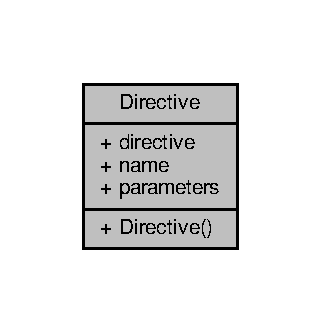
\includegraphics[width=154pt]{classft_1_1_directive__coll__graph}
\end{center}
\end{figure}
\subsection*{Public Member Functions}
\begin{DoxyCompactItemize}
\item 
\hyperlink{classft_1_1_directive_aedcc052461811957b6a8610e0c72968d}{Directive} (enum \hyperlink{namespaceft_a5a5554dff10f0dc50bae4cc5825ad75d}{Directive\+Kind} \hyperlink{classft_1_1_directive_ad974f853279afa5ad30a28773b94fe87}{directive}=\hyperlink{namespaceft_a5a5554dff10f0dc50bae4cc5825ad75da67e044074f46e6cea22788527da5f02e}{H\+T\+TP}, const std\+::string \&\hyperlink{classft_1_1_directive_a9b45b3e13bd9167aab02e17e08916231}{name}=std\+::string())
\end{DoxyCompactItemize}
\subsection*{Public Attributes}
\begin{DoxyCompactItemize}
\item 
enum \hyperlink{namespaceft_a5a5554dff10f0dc50bae4cc5825ad75d}{Directive\+Kind} \hyperlink{classft_1_1_directive_ad974f853279afa5ad30a28773b94fe87}{directive}
\item 
std\+::string \hyperlink{classft_1_1_directive_a9b45b3e13bd9167aab02e17e08916231}{name}
\item 
std\+::vector$<$ std\+::string $>$ \hyperlink{classft_1_1_directive_a2197fbfab6b0ae80e5599c8ddc562479}{parameters}
\end{DoxyCompactItemize}


\subsection{Detailed Description}


Definition at line 49 of file Directive.\+hpp.



\subsection{Constructor \& Destructor Documentation}
\mbox{\Hypertarget{classft_1_1_directive_aedcc052461811957b6a8610e0c72968d}\label{classft_1_1_directive_aedcc052461811957b6a8610e0c72968d}} 
\index{ft\+::\+Directive@{ft\+::\+Directive}!Directive@{Directive}}
\index{Directive@{Directive}!ft\+::\+Directive@{ft\+::\+Directive}}
\subsubsection{\texorpdfstring{Directive()}{Directive()}}
{\footnotesize\ttfamily \hyperlink{classft_1_1_directive}{Directive} (\begin{DoxyParamCaption}\item[{enum \hyperlink{namespaceft_a5a5554dff10f0dc50bae4cc5825ad75d}{Directive\+Kind}}]{directive = {\ttfamily \hyperlink{namespaceft_a5a5554dff10f0dc50bae4cc5825ad75da67e044074f46e6cea22788527da5f02e}{H\+T\+TP}},  }\item[{const std\+::string \&}]{name = {\ttfamily std\+:\+:string()} }\end{DoxyParamCaption})\hspace{0.3cm}{\ttfamily [inline]}}



Definition at line 57 of file Directive.\+hpp.


\begin{DoxyCode}
57 : \hyperlink{classft_1_1_directive_ad974f853279afa5ad30a28773b94fe87}{directive}(\hyperlink{classft_1_1_directive_ad974f853279afa5ad30a28773b94fe87}{directive}), \hyperlink{classft_1_1_directive_a9b45b3e13bd9167aab02e17e08916231}{name}(\hyperlink{classft_1_1_directive_a9b45b3e13bd9167aab02e17e08916231}{name}) \{\}
\end{DoxyCode}


\subsection{Member Data Documentation}
\mbox{\Hypertarget{classft_1_1_directive_ad974f853279afa5ad30a28773b94fe87}\label{classft_1_1_directive_ad974f853279afa5ad30a28773b94fe87}} 
\index{ft\+::\+Directive@{ft\+::\+Directive}!directive@{directive}}
\index{directive@{directive}!ft\+::\+Directive@{ft\+::\+Directive}}
\subsubsection{\texorpdfstring{directive}{directive}}
{\footnotesize\ttfamily enum \hyperlink{namespaceft_a5a5554dff10f0dc50bae4cc5825ad75d}{Directive\+Kind} directive}



Definition at line 52 of file Directive.\+hpp.

\mbox{\Hypertarget{classft_1_1_directive_a9b45b3e13bd9167aab02e17e08916231}\label{classft_1_1_directive_a9b45b3e13bd9167aab02e17e08916231}} 
\index{ft\+::\+Directive@{ft\+::\+Directive}!name@{name}}
\index{name@{name}!ft\+::\+Directive@{ft\+::\+Directive}}
\subsubsection{\texorpdfstring{name}{name}}
{\footnotesize\ttfamily std\+::string name}



Definition at line 53 of file Directive.\+hpp.

\mbox{\Hypertarget{classft_1_1_directive_a2197fbfab6b0ae80e5599c8ddc562479}\label{classft_1_1_directive_a2197fbfab6b0ae80e5599c8ddc562479}} 
\index{ft\+::\+Directive@{ft\+::\+Directive}!parameters@{parameters}}
\index{parameters@{parameters}!ft\+::\+Directive@{ft\+::\+Directive}}
\subsubsection{\texorpdfstring{parameters}{parameters}}
{\footnotesize\ttfamily std\+::vector$<$std\+::string$>$ parameters}



Definition at line 54 of file Directive.\+hpp.



The documentation for this class was generated from the following file\+:\begin{DoxyCompactItemize}
\item 
/home/cjung-\/mo/\+Documents/42/\+Webserv/config/src/\hyperlink{_directive_8hpp}{Directive.\+hpp}\end{DoxyCompactItemize}

\hypertarget{classft_1_1_http_block}{}\section{Http\+Block Class Reference}
\label{classft_1_1_http_block}\index{Http\+Block@{Http\+Block}}


{\ttfamily \#include $<$Http\+Block.\+hpp$>$}



Inheritance diagram for Http\+Block\+:
\nopagebreak
\begin{figure}[H]
\begin{center}
\leavevmode
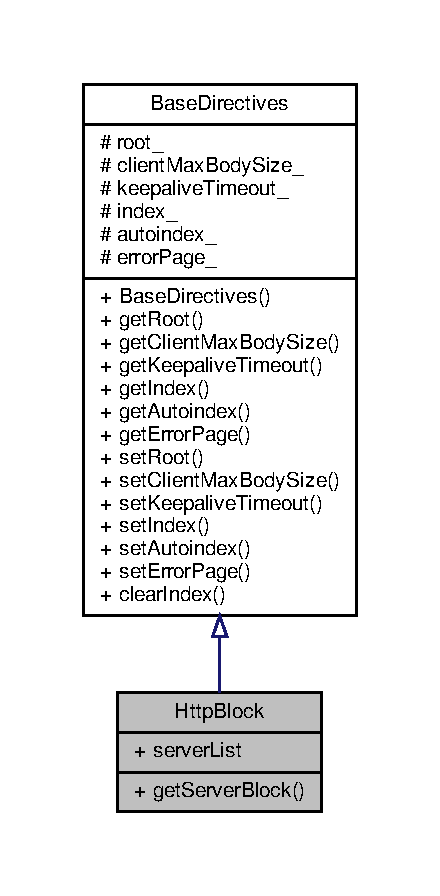
\includegraphics[width=211pt]{classft_1_1_http_block__inherit__graph}
\end{center}
\end{figure}


Collaboration diagram for Http\+Block\+:
\nopagebreak
\begin{figure}[H]
\begin{center}
\leavevmode
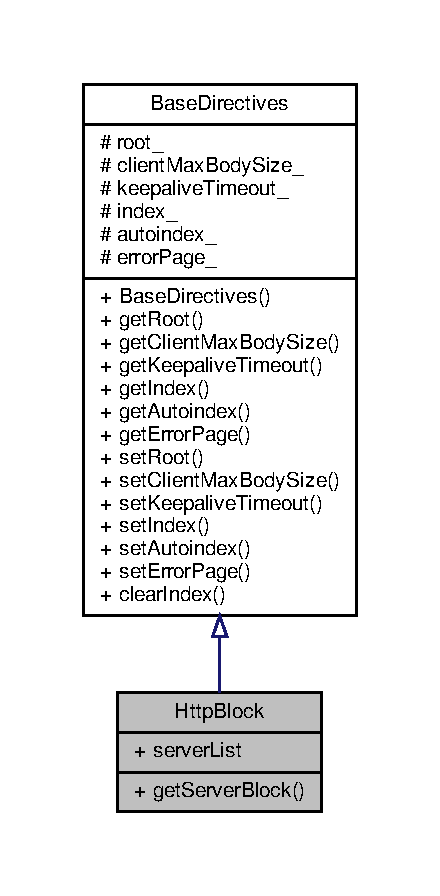
\includegraphics[width=211pt]{classft_1_1_http_block__coll__graph}
\end{center}
\end{figure}
\subsection*{Public Member Functions}
\begin{DoxyCompactItemize}
\item 
std\+::vector$<$ \hyperlink{classft_1_1_server_block}{Server\+Block} $>$ \hyperlink{classft_1_1_http_block_a44c1fe5ff1e2f7b609de503771d5344b}{get\+Server\+Block} () const
\item 
const std\+::string \hyperlink{classft_1_1_base_directives_aa5dbcb08bda0a0e7e502d2df7cf64287}{get\+Root} (void) const
\item 
unsigned long \hyperlink{classft_1_1_base_directives_a930398ba1e4b99b2ba01a60dcda0c923}{get\+Client\+Max\+Body\+Size} (void) const
\item 
unsigned int \hyperlink{classft_1_1_base_directives_ab8574338758f65325cab5d1c394826c8}{get\+Keepalive\+Timeout} (void) const
\item 
const std\+::vector$<$ std\+::string $>$ \hyperlink{classft_1_1_base_directives_a018f34a5ffd66e891494b5c0ee69177b}{get\+Index} (void) const
\item 
bool \hyperlink{classft_1_1_base_directives_a4c11ed7ad76aeac228b029a2444de568}{get\+Autoindex} (void) const
\item 
const std\+::string \hyperlink{classft_1_1_base_directives_a3cb0c21f17781de392d5ee09d7190caf}{get\+Error\+Page} (void) const
\item 
void \hyperlink{classft_1_1_base_directives_a2a7990e309f7e38f2915dbbb0d2704cf}{set\+Root} (const std\+::string x)
\item 
void \hyperlink{classft_1_1_base_directives_a39bf4922f3236043c76beaffaa557a3b}{set\+Client\+Max\+Body\+Size} (const unsigned long x)
\item 
void \hyperlink{classft_1_1_base_directives_a0818b8529872ba9622329e2118d20c39}{set\+Keepalive\+Timeout} (const unsigned int x)
\item 
void \hyperlink{classft_1_1_base_directives_a6d3d8fd6eaaf71304128af6b3cee2a69}{set\+Index} (const std\+::string x)
\item 
void \hyperlink{classft_1_1_base_directives_ae7293c7bbf34e9bdc60c540dccd53342}{set\+Autoindex} (const bool x)
\item 
void \hyperlink{classft_1_1_base_directives_a505ecc88b3e1779583ad60cc243c7769}{set\+Error\+Page} (const std\+::string x)
\item 
void \hyperlink{classft_1_1_base_directives_a36d96dc74e650162c25a325813130ab2}{clear\+Index} (void)
\end{DoxyCompactItemize}
\subsection*{Public Attributes}
\begin{DoxyCompactItemize}
\item 
std\+::vector$<$ \hyperlink{classft_1_1_server_block}{Server\+Block} $>$ \hyperlink{classft_1_1_http_block_ad832a81fa84d149a58e896f2036cd53b}{server\+List}
\end{DoxyCompactItemize}
\subsection*{Protected Attributes}
\begin{DoxyCompactItemize}
\item 
std\+::string \hyperlink{classft_1_1_base_directives_abb1eaf0bba10b90172d6152e69457dc7}{root\+\_\+}
\item 
unsigned long \hyperlink{classft_1_1_base_directives_ad65c2594d2a90ca065d410dfd4066a19}{client\+Max\+Body\+Size\+\_\+}
\item 
unsigned int \hyperlink{classft_1_1_base_directives_aa1f5f394b428d0d18765a9b9e14e648f}{keepalive\+Timeout\+\_\+}
\item 
std\+::vector$<$ std\+::string $>$ \hyperlink{classft_1_1_base_directives_a6ba30626837f300201cd32c35d50aa49}{index\+\_\+}
\item 
bool \hyperlink{classft_1_1_base_directives_a4ebffbe32f50a462afa139c6f03c1a4f}{autoindex\+\_\+}
\item 
std\+::string \hyperlink{classft_1_1_base_directives_a5c0d388109f086503961de84fe3fce90}{error\+Page\+\_\+}
\end{DoxyCompactItemize}


\subsection{Detailed Description}


Definition at line 10 of file Http\+Block.\+hpp.



\subsection{Member Function Documentation}
\mbox{\Hypertarget{classft_1_1_base_directives_a36d96dc74e650162c25a325813130ab2}\label{classft_1_1_base_directives_a36d96dc74e650162c25a325813130ab2}} 
\index{ft\+::\+Http\+Block@{ft\+::\+Http\+Block}!clear\+Index@{clear\+Index}}
\index{clear\+Index@{clear\+Index}!ft\+::\+Http\+Block@{ft\+::\+Http\+Block}}
\subsubsection{\texorpdfstring{clear\+Index()}{clearIndex()}}
{\footnotesize\ttfamily void clear\+Index (\begin{DoxyParamCaption}\item[{void}]{ }\end{DoxyParamCaption})\hspace{0.3cm}{\ttfamily [inherited]}}



Definition at line 78 of file Base\+Directives.\+cpp.


\begin{DoxyCode}
79     \{
80         this->\hyperlink{classft_1_1_base_directives_a6ba30626837f300201cd32c35d50aa49}{index\_}.clear();
81     \}
\end{DoxyCode}
Here is the caller graph for this function\+:
\nopagebreak
\begin{figure}[H]
\begin{center}
\leavevmode
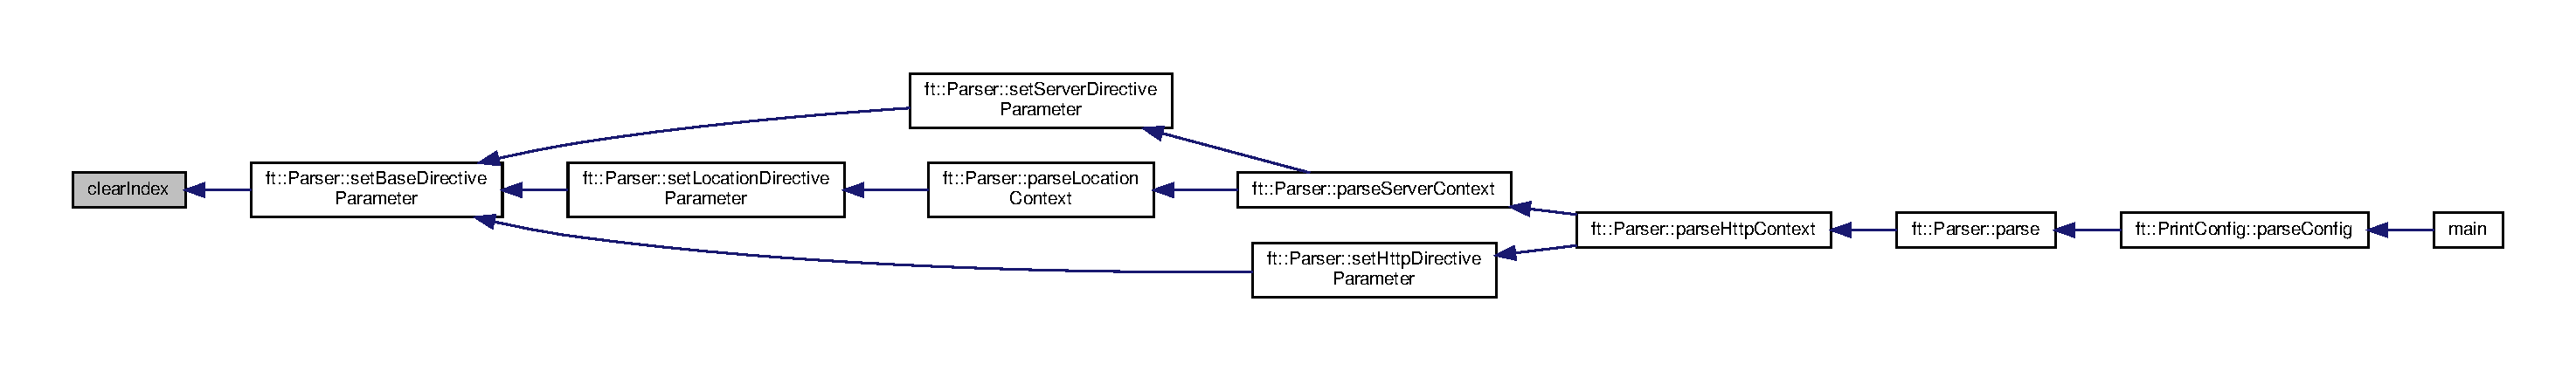
\includegraphics[width=350pt]{classft_1_1_base_directives_a36d96dc74e650162c25a325813130ab2_icgraph}
\end{center}
\end{figure}
\mbox{\Hypertarget{classft_1_1_base_directives_a4c11ed7ad76aeac228b029a2444de568}\label{classft_1_1_base_directives_a4c11ed7ad76aeac228b029a2444de568}} 
\index{ft\+::\+Http\+Block@{ft\+::\+Http\+Block}!get\+Autoindex@{get\+Autoindex}}
\index{get\+Autoindex@{get\+Autoindex}!ft\+::\+Http\+Block@{ft\+::\+Http\+Block}}
\subsubsection{\texorpdfstring{get\+Autoindex()}{getAutoindex()}}
{\footnotesize\ttfamily bool get\+Autoindex (\begin{DoxyParamCaption}\item[{void}]{ }\end{DoxyParamCaption}) const\hspace{0.3cm}{\ttfamily [inherited]}}



Definition at line 36 of file Base\+Directives.\+cpp.


\begin{DoxyCode}
37     \{
38         \textcolor{keywordflow}{return} (this->\hyperlink{classft_1_1_base_directives_a4ebffbe32f50a462afa139c6f03c1a4f}{autoindex\_});
39     \}
\end{DoxyCode}
Here is the caller graph for this function\+:
\nopagebreak
\begin{figure}[H]
\begin{center}
\leavevmode
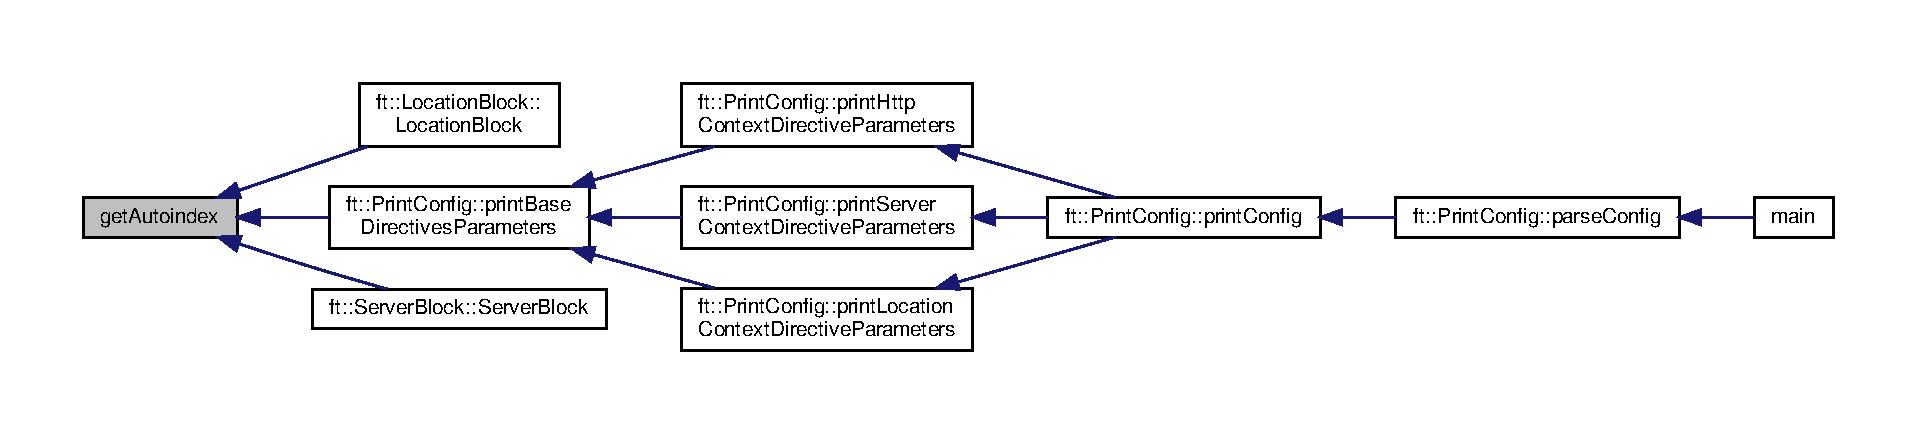
\includegraphics[width=350pt]{classft_1_1_base_directives_a4c11ed7ad76aeac228b029a2444de568_icgraph}
\end{center}
\end{figure}
\mbox{\Hypertarget{classft_1_1_base_directives_a930398ba1e4b99b2ba01a60dcda0c923}\label{classft_1_1_base_directives_a930398ba1e4b99b2ba01a60dcda0c923}} 
\index{ft\+::\+Http\+Block@{ft\+::\+Http\+Block}!get\+Client\+Max\+Body\+Size@{get\+Client\+Max\+Body\+Size}}
\index{get\+Client\+Max\+Body\+Size@{get\+Client\+Max\+Body\+Size}!ft\+::\+Http\+Block@{ft\+::\+Http\+Block}}
\subsubsection{\texorpdfstring{get\+Client\+Max\+Body\+Size()}{getClientMaxBodySize()}}
{\footnotesize\ttfamily unsigned long get\+Client\+Max\+Body\+Size (\begin{DoxyParamCaption}\item[{void}]{ }\end{DoxyParamCaption}) const\hspace{0.3cm}{\ttfamily [inherited]}}



Definition at line 21 of file Base\+Directives.\+cpp.


\begin{DoxyCode}
22     \{
23         \textcolor{keywordflow}{return} (this->\hyperlink{classft_1_1_base_directives_ad65c2594d2a90ca065d410dfd4066a19}{clientMaxBodySize\_});
24     \}
\end{DoxyCode}
Here is the caller graph for this function\+:
\nopagebreak
\begin{figure}[H]
\begin{center}
\leavevmode
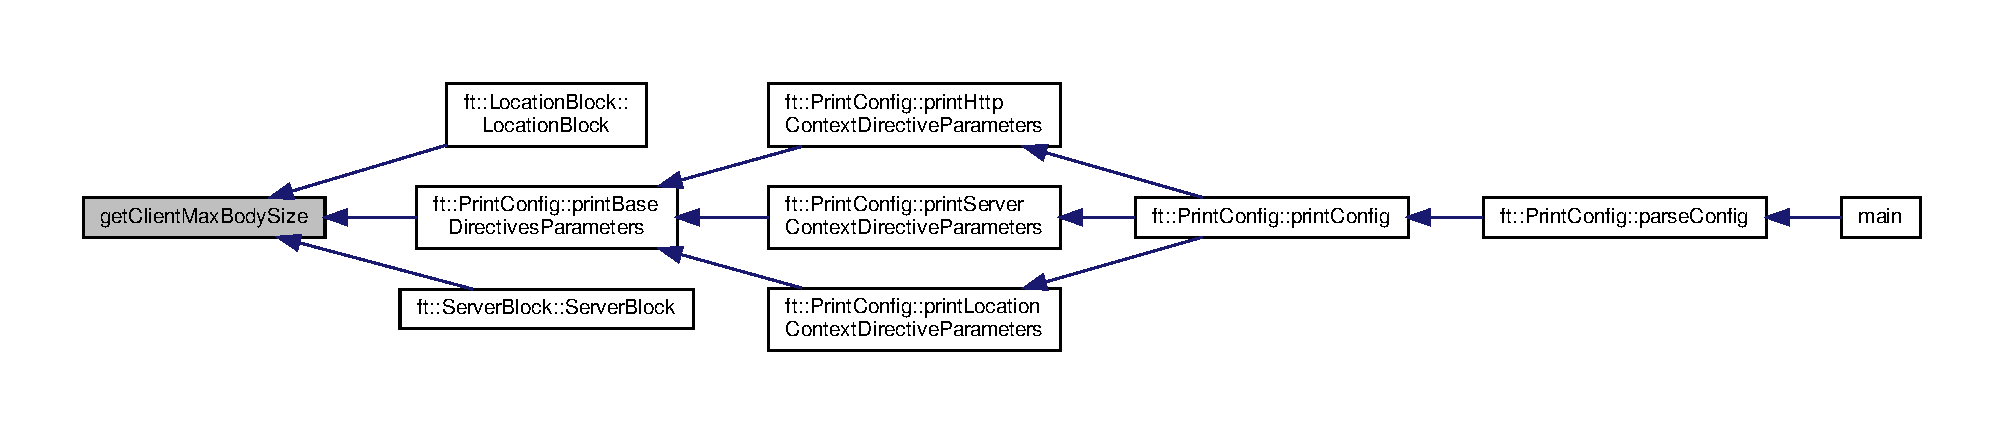
\includegraphics[width=350pt]{classft_1_1_base_directives_a930398ba1e4b99b2ba01a60dcda0c923_icgraph}
\end{center}
\end{figure}
\mbox{\Hypertarget{classft_1_1_base_directives_a3cb0c21f17781de392d5ee09d7190caf}\label{classft_1_1_base_directives_a3cb0c21f17781de392d5ee09d7190caf}} 
\index{ft\+::\+Http\+Block@{ft\+::\+Http\+Block}!get\+Error\+Page@{get\+Error\+Page}}
\index{get\+Error\+Page@{get\+Error\+Page}!ft\+::\+Http\+Block@{ft\+::\+Http\+Block}}
\subsubsection{\texorpdfstring{get\+Error\+Page()}{getErrorPage()}}
{\footnotesize\ttfamily const std\+::string get\+Error\+Page (\begin{DoxyParamCaption}\item[{void}]{ }\end{DoxyParamCaption}) const\hspace{0.3cm}{\ttfamily [inherited]}}



Definition at line 41 of file Base\+Directives.\+cpp.


\begin{DoxyCode}
42     \{
43         \textcolor{keywordflow}{return} (this->\hyperlink{classft_1_1_base_directives_a5c0d388109f086503961de84fe3fce90}{errorPage\_});
44     \}
\end{DoxyCode}
Here is the caller graph for this function\+:
\nopagebreak
\begin{figure}[H]
\begin{center}
\leavevmode
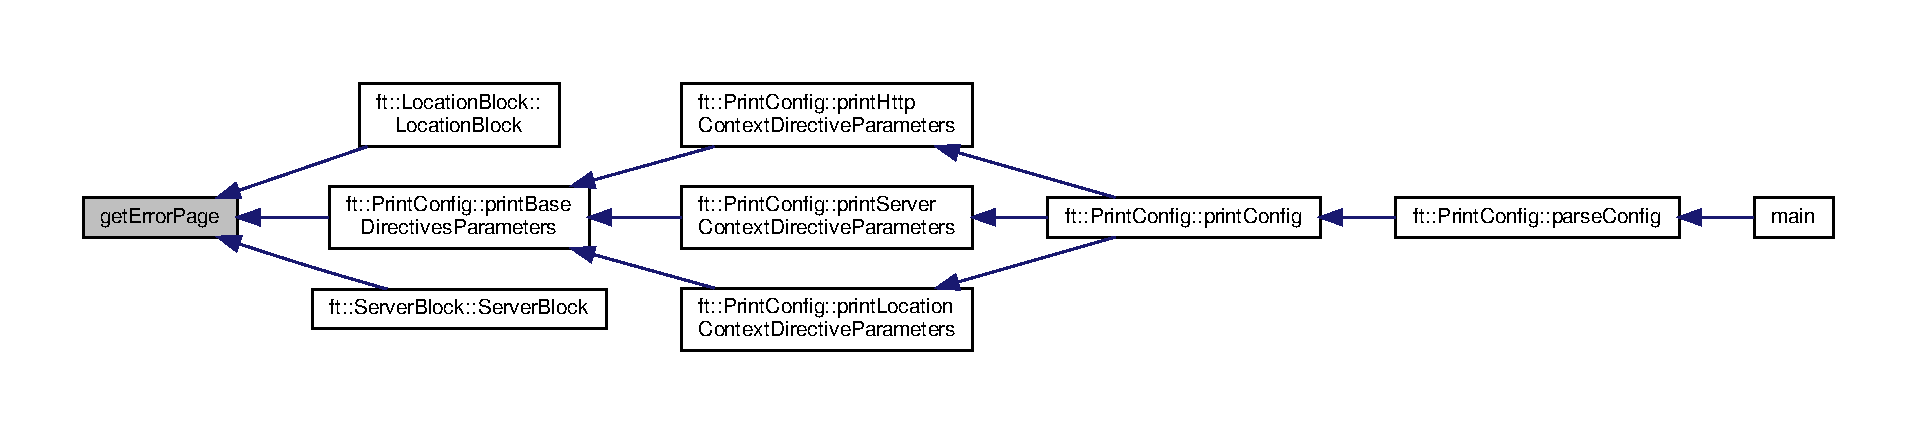
\includegraphics[width=350pt]{classft_1_1_base_directives_a3cb0c21f17781de392d5ee09d7190caf_icgraph}
\end{center}
\end{figure}
\mbox{\Hypertarget{classft_1_1_base_directives_a018f34a5ffd66e891494b5c0ee69177b}\label{classft_1_1_base_directives_a018f34a5ffd66e891494b5c0ee69177b}} 
\index{ft\+::\+Http\+Block@{ft\+::\+Http\+Block}!get\+Index@{get\+Index}}
\index{get\+Index@{get\+Index}!ft\+::\+Http\+Block@{ft\+::\+Http\+Block}}
\subsubsection{\texorpdfstring{get\+Index()}{getIndex()}}
{\footnotesize\ttfamily const std\+::vector$<$ std\+::string $>$ get\+Index (\begin{DoxyParamCaption}\item[{void}]{ }\end{DoxyParamCaption}) const\hspace{0.3cm}{\ttfamily [inherited]}}



Definition at line 31 of file Base\+Directives.\+cpp.


\begin{DoxyCode}
32     \{
33         \textcolor{keywordflow}{return} (this->\hyperlink{classft_1_1_base_directives_a6ba30626837f300201cd32c35d50aa49}{index\_});
34     \}
\end{DoxyCode}
Here is the caller graph for this function\+:
\nopagebreak
\begin{figure}[H]
\begin{center}
\leavevmode
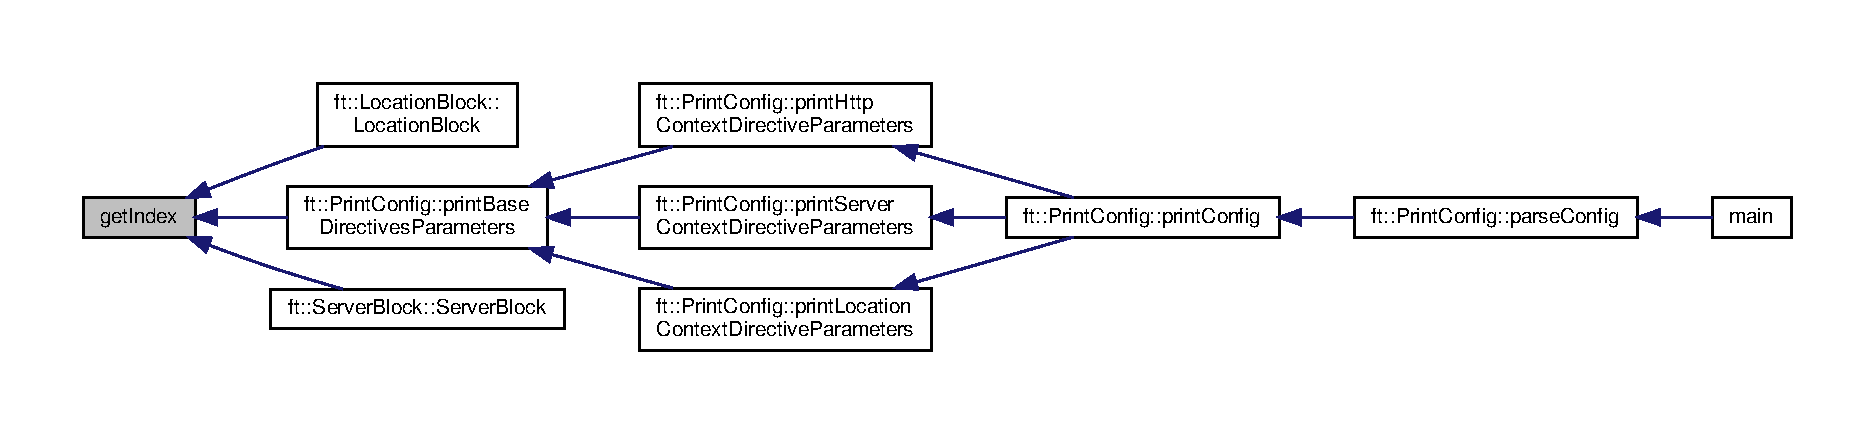
\includegraphics[width=350pt]{classft_1_1_base_directives_a018f34a5ffd66e891494b5c0ee69177b_icgraph}
\end{center}
\end{figure}
\mbox{\Hypertarget{classft_1_1_base_directives_ab8574338758f65325cab5d1c394826c8}\label{classft_1_1_base_directives_ab8574338758f65325cab5d1c394826c8}} 
\index{ft\+::\+Http\+Block@{ft\+::\+Http\+Block}!get\+Keepalive\+Timeout@{get\+Keepalive\+Timeout}}
\index{get\+Keepalive\+Timeout@{get\+Keepalive\+Timeout}!ft\+::\+Http\+Block@{ft\+::\+Http\+Block}}
\subsubsection{\texorpdfstring{get\+Keepalive\+Timeout()}{getKeepaliveTimeout()}}
{\footnotesize\ttfamily unsigned int get\+Keepalive\+Timeout (\begin{DoxyParamCaption}\item[{void}]{ }\end{DoxyParamCaption}) const\hspace{0.3cm}{\ttfamily [inherited]}}



Definition at line 26 of file Base\+Directives.\+cpp.


\begin{DoxyCode}
27     \{
28         \textcolor{keywordflow}{return} (this->\hyperlink{classft_1_1_base_directives_aa1f5f394b428d0d18765a9b9e14e648f}{keepaliveTimeout\_});
29     \}
\end{DoxyCode}
Here is the caller graph for this function\+:
\nopagebreak
\begin{figure}[H]
\begin{center}
\leavevmode
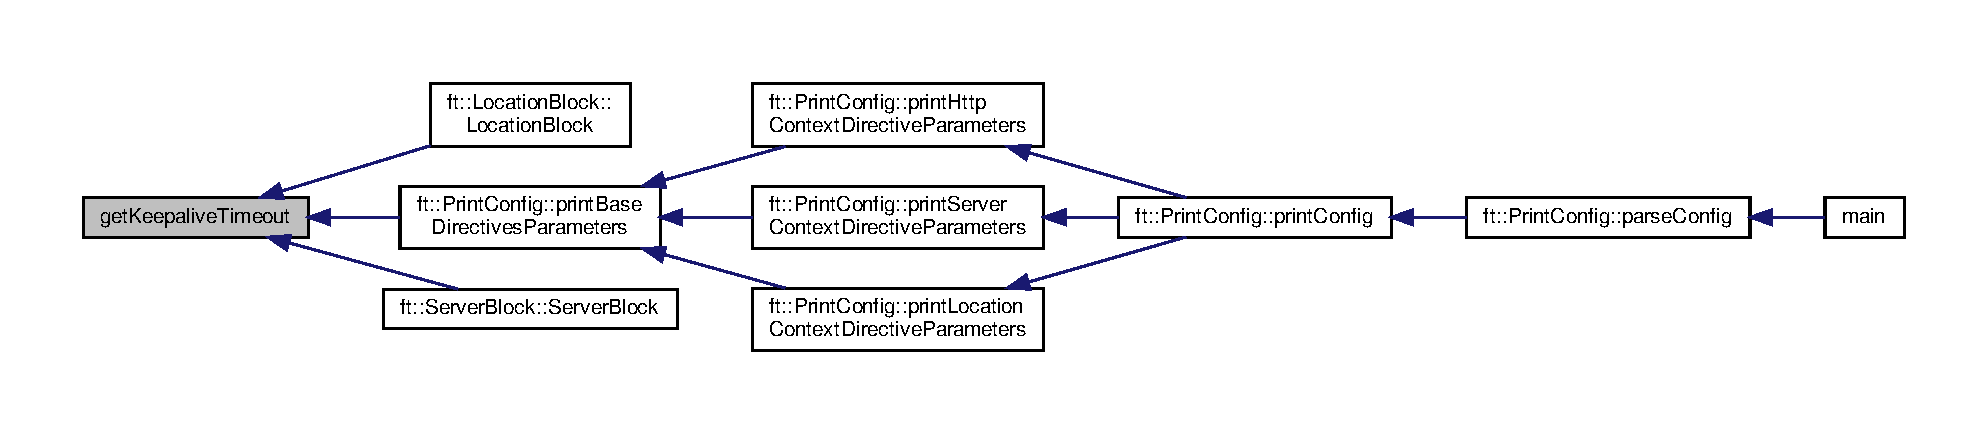
\includegraphics[width=350pt]{classft_1_1_base_directives_ab8574338758f65325cab5d1c394826c8_icgraph}
\end{center}
\end{figure}
\mbox{\Hypertarget{classft_1_1_base_directives_aa5dbcb08bda0a0e7e502d2df7cf64287}\label{classft_1_1_base_directives_aa5dbcb08bda0a0e7e502d2df7cf64287}} 
\index{ft\+::\+Http\+Block@{ft\+::\+Http\+Block}!get\+Root@{get\+Root}}
\index{get\+Root@{get\+Root}!ft\+::\+Http\+Block@{ft\+::\+Http\+Block}}
\subsubsection{\texorpdfstring{get\+Root()}{getRoot()}}
{\footnotesize\ttfamily const std\+::string get\+Root (\begin{DoxyParamCaption}\item[{void}]{ }\end{DoxyParamCaption}) const\hspace{0.3cm}{\ttfamily [inherited]}}



Definition at line 16 of file Base\+Directives.\+cpp.


\begin{DoxyCode}
17     \{
18         \textcolor{keywordflow}{return} (this->\hyperlink{classft_1_1_base_directives_abb1eaf0bba10b90172d6152e69457dc7}{root\_});
19     \}
\end{DoxyCode}
Here is the caller graph for this function\+:
\nopagebreak
\begin{figure}[H]
\begin{center}
\leavevmode
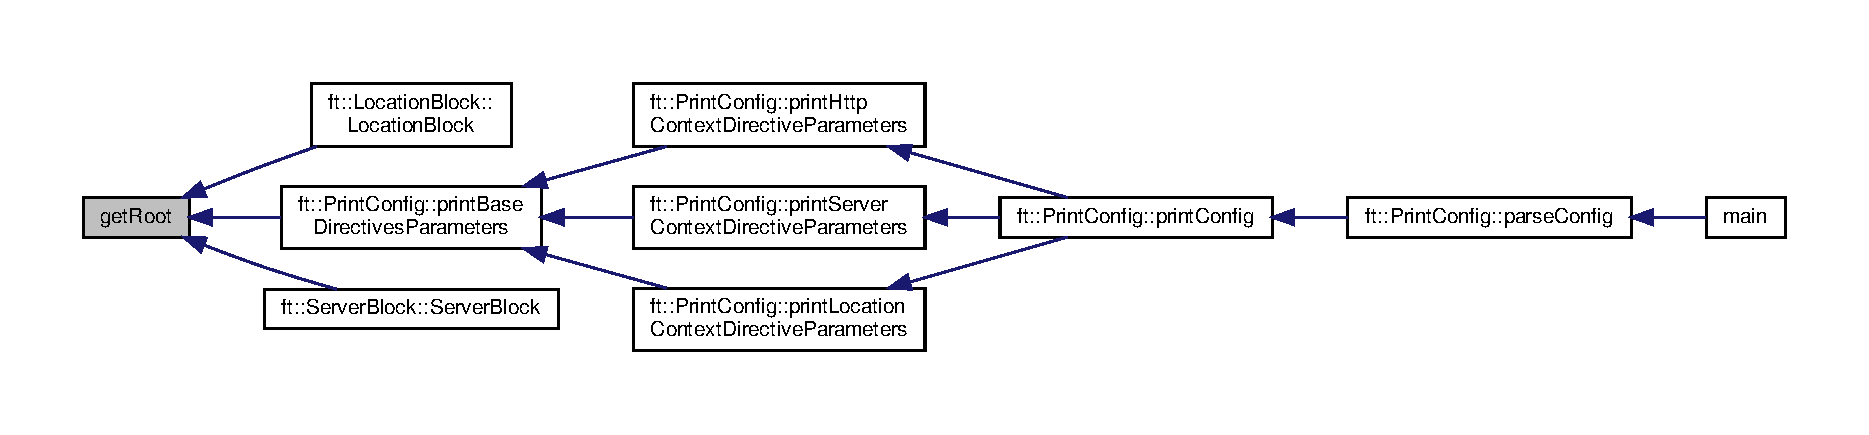
\includegraphics[width=350pt]{classft_1_1_base_directives_aa5dbcb08bda0a0e7e502d2df7cf64287_icgraph}
\end{center}
\end{figure}
\mbox{\Hypertarget{classft_1_1_http_block_a44c1fe5ff1e2f7b609de503771d5344b}\label{classft_1_1_http_block_a44c1fe5ff1e2f7b609de503771d5344b}} 
\index{ft\+::\+Http\+Block@{ft\+::\+Http\+Block}!get\+Server\+Block@{get\+Server\+Block}}
\index{get\+Server\+Block@{get\+Server\+Block}!ft\+::\+Http\+Block@{ft\+::\+Http\+Block}}
\subsubsection{\texorpdfstring{get\+Server\+Block()}{getServerBlock()}}
{\footnotesize\ttfamily std\+::vector$<$ \hyperlink{classft_1_1_server_block}{Server\+Block} $>$ get\+Server\+Block (\begin{DoxyParamCaption}{ }\end{DoxyParamCaption}) const}



Definition at line 5 of file Http\+Block.\+cpp.


\begin{DoxyCode}
6     \{
7         \textcolor{keywordflow}{return} (this->\hyperlink{classft_1_1_http_block_ad832a81fa84d149a58e896f2036cd53b}{serverList});
8     \}
\end{DoxyCode}
\mbox{\Hypertarget{classft_1_1_base_directives_ae7293c7bbf34e9bdc60c540dccd53342}\label{classft_1_1_base_directives_ae7293c7bbf34e9bdc60c540dccd53342}} 
\index{ft\+::\+Http\+Block@{ft\+::\+Http\+Block}!set\+Autoindex@{set\+Autoindex}}
\index{set\+Autoindex@{set\+Autoindex}!ft\+::\+Http\+Block@{ft\+::\+Http\+Block}}
\subsubsection{\texorpdfstring{set\+Autoindex()}{setAutoindex()}}
{\footnotesize\ttfamily void set\+Autoindex (\begin{DoxyParamCaption}\item[{const bool}]{x }\end{DoxyParamCaption})\hspace{0.3cm}{\ttfamily [inherited]}}



Definition at line 67 of file Base\+Directives.\+cpp.


\begin{DoxyCode}
68     \{
69         this->\hyperlink{classft_1_1_base_directives_a4ebffbe32f50a462afa139c6f03c1a4f}{autoindex\_} = x;
70     \}
\end{DoxyCode}
Here is the caller graph for this function\+:\nopagebreak
\begin{figure}[H]
\begin{center}
\leavevmode
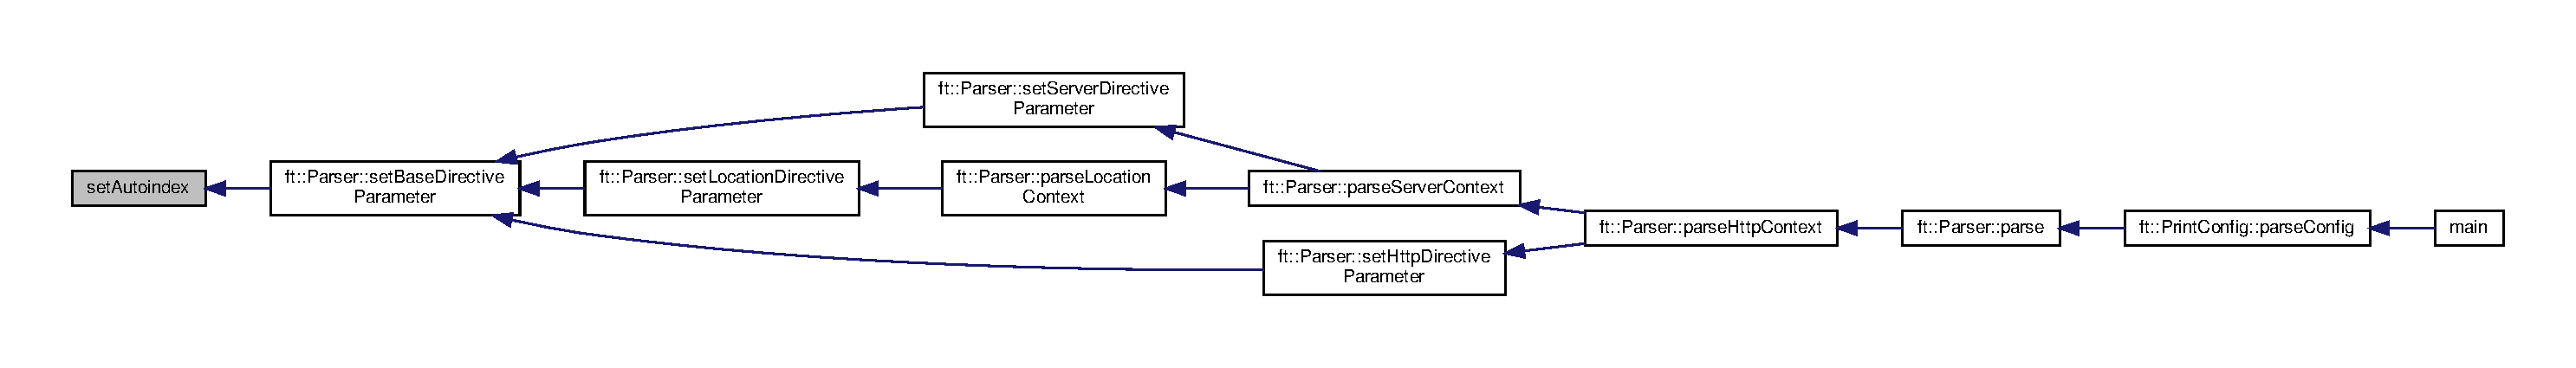
\includegraphics[width=350pt]{classft_1_1_base_directives_ae7293c7bbf34e9bdc60c540dccd53342_icgraph}
\end{center}
\end{figure}
\mbox{\Hypertarget{classft_1_1_base_directives_a39bf4922f3236043c76beaffaa557a3b}\label{classft_1_1_base_directives_a39bf4922f3236043c76beaffaa557a3b}} 
\index{ft\+::\+Http\+Block@{ft\+::\+Http\+Block}!set\+Client\+Max\+Body\+Size@{set\+Client\+Max\+Body\+Size}}
\index{set\+Client\+Max\+Body\+Size@{set\+Client\+Max\+Body\+Size}!ft\+::\+Http\+Block@{ft\+::\+Http\+Block}}
\subsubsection{\texorpdfstring{set\+Client\+Max\+Body\+Size()}{setClientMaxBodySize()}}
{\footnotesize\ttfamily void set\+Client\+Max\+Body\+Size (\begin{DoxyParamCaption}\item[{const unsigned long}]{x }\end{DoxyParamCaption})\hspace{0.3cm}{\ttfamily [inherited]}}



Definition at line 52 of file Base\+Directives.\+cpp.


\begin{DoxyCode}
53     \{
54         this->\hyperlink{classft_1_1_base_directives_ad65c2594d2a90ca065d410dfd4066a19}{clientMaxBodySize\_} = x;
55     \}
\end{DoxyCode}
Here is the caller graph for this function\+:\nopagebreak
\begin{figure}[H]
\begin{center}
\leavevmode
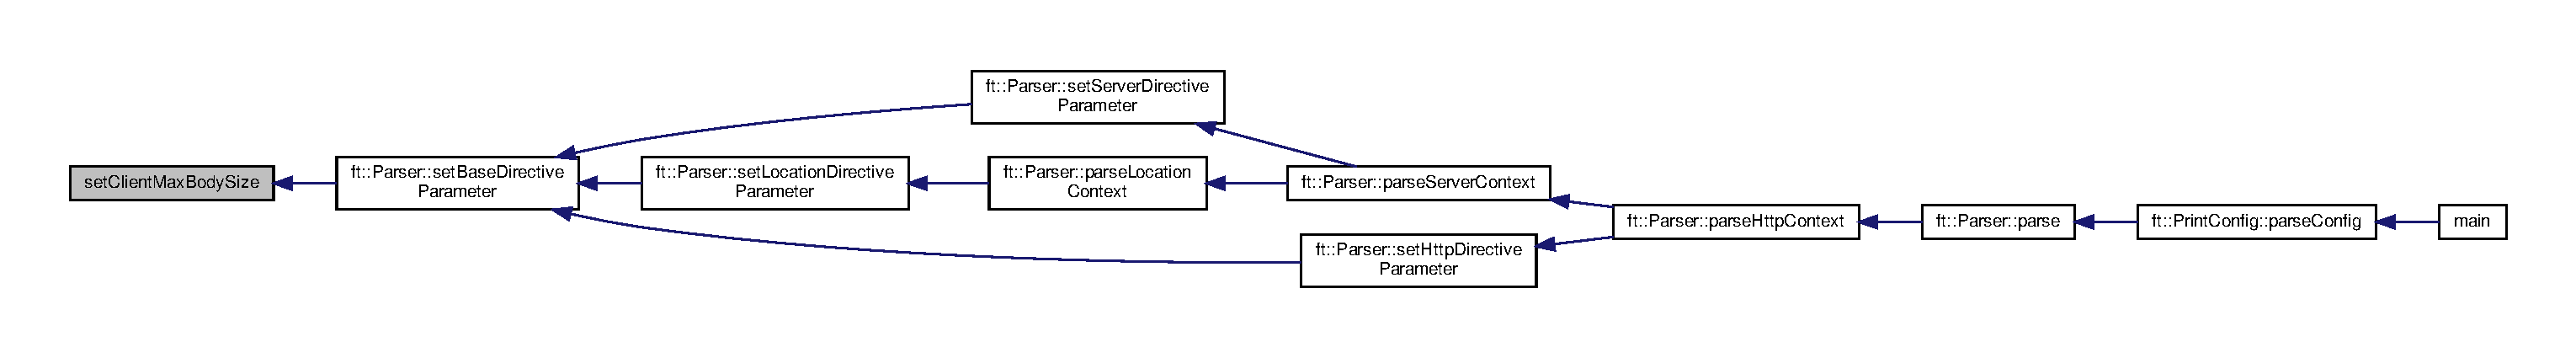
\includegraphics[width=350pt]{classft_1_1_base_directives_a39bf4922f3236043c76beaffaa557a3b_icgraph}
\end{center}
\end{figure}
\mbox{\Hypertarget{classft_1_1_base_directives_a505ecc88b3e1779583ad60cc243c7769}\label{classft_1_1_base_directives_a505ecc88b3e1779583ad60cc243c7769}} 
\index{ft\+::\+Http\+Block@{ft\+::\+Http\+Block}!set\+Error\+Page@{set\+Error\+Page}}
\index{set\+Error\+Page@{set\+Error\+Page}!ft\+::\+Http\+Block@{ft\+::\+Http\+Block}}
\subsubsection{\texorpdfstring{set\+Error\+Page()}{setErrorPage()}}
{\footnotesize\ttfamily void set\+Error\+Page (\begin{DoxyParamCaption}\item[{const std\+::string}]{x }\end{DoxyParamCaption})\hspace{0.3cm}{\ttfamily [inherited]}}



Definition at line 72 of file Base\+Directives.\+cpp.


\begin{DoxyCode}
73     \{
74         this->\hyperlink{classft_1_1_base_directives_a5c0d388109f086503961de84fe3fce90}{errorPage\_} = x;
75     \}
\end{DoxyCode}
Here is the caller graph for this function\+:\nopagebreak
\begin{figure}[H]
\begin{center}
\leavevmode
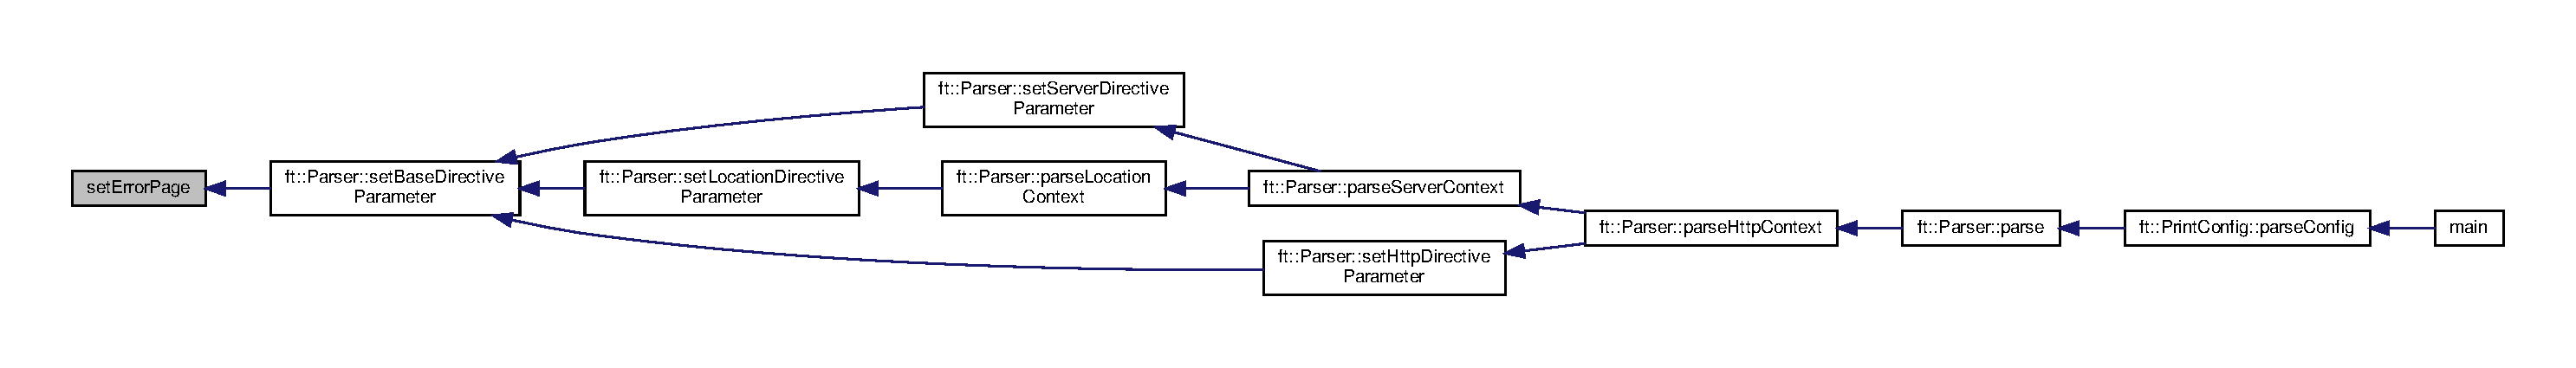
\includegraphics[width=350pt]{classft_1_1_base_directives_a505ecc88b3e1779583ad60cc243c7769_icgraph}
\end{center}
\end{figure}
\mbox{\Hypertarget{classft_1_1_base_directives_a6d3d8fd6eaaf71304128af6b3cee2a69}\label{classft_1_1_base_directives_a6d3d8fd6eaaf71304128af6b3cee2a69}} 
\index{ft\+::\+Http\+Block@{ft\+::\+Http\+Block}!set\+Index@{set\+Index}}
\index{set\+Index@{set\+Index}!ft\+::\+Http\+Block@{ft\+::\+Http\+Block}}
\subsubsection{\texorpdfstring{set\+Index()}{setIndex()}}
{\footnotesize\ttfamily void set\+Index (\begin{DoxyParamCaption}\item[{const std\+::string}]{x }\end{DoxyParamCaption})\hspace{0.3cm}{\ttfamily [inherited]}}



Definition at line 62 of file Base\+Directives.\+cpp.


\begin{DoxyCode}
63     \{
64         this->\hyperlink{classft_1_1_base_directives_a6ba30626837f300201cd32c35d50aa49}{index\_}.push\_back(x);
65     \}
\end{DoxyCode}
Here is the caller graph for this function\+:\nopagebreak
\begin{figure}[H]
\begin{center}
\leavevmode
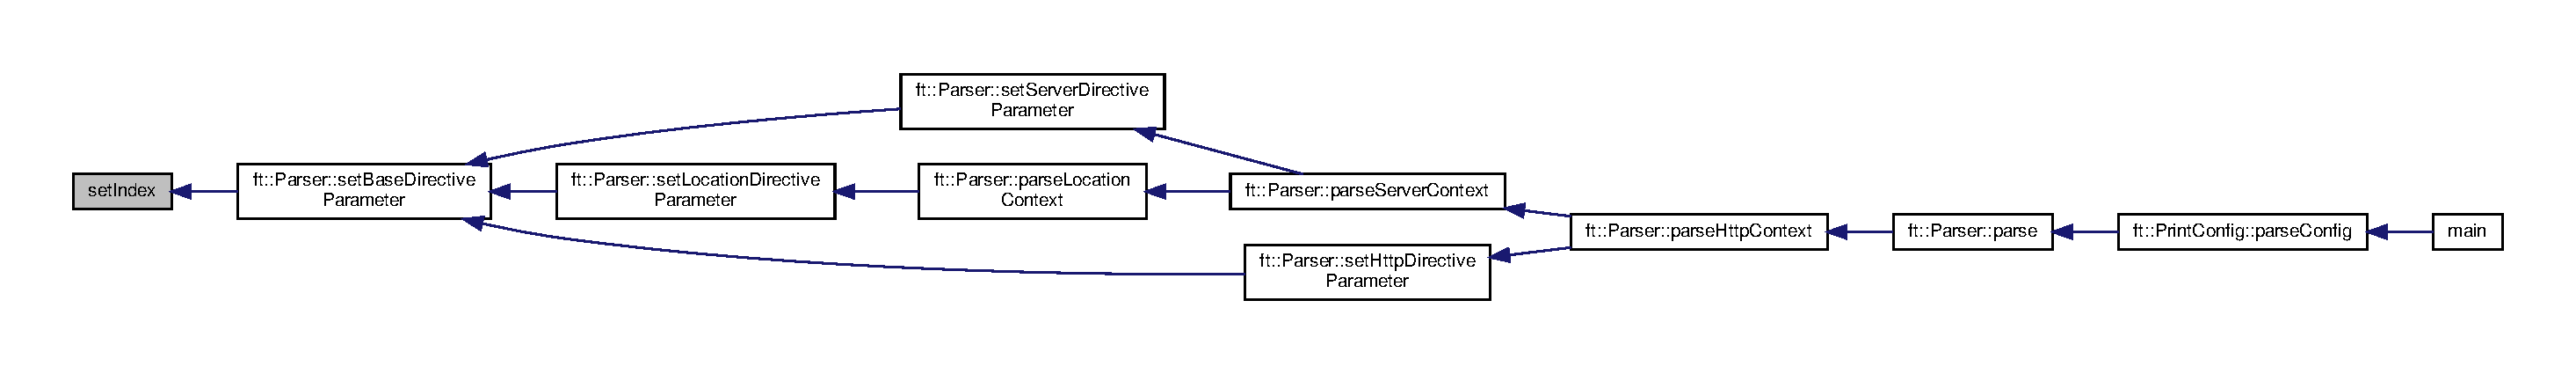
\includegraphics[width=350pt]{classft_1_1_base_directives_a6d3d8fd6eaaf71304128af6b3cee2a69_icgraph}
\end{center}
\end{figure}
\mbox{\Hypertarget{classft_1_1_base_directives_a0818b8529872ba9622329e2118d20c39}\label{classft_1_1_base_directives_a0818b8529872ba9622329e2118d20c39}} 
\index{ft\+::\+Http\+Block@{ft\+::\+Http\+Block}!set\+Keepalive\+Timeout@{set\+Keepalive\+Timeout}}
\index{set\+Keepalive\+Timeout@{set\+Keepalive\+Timeout}!ft\+::\+Http\+Block@{ft\+::\+Http\+Block}}
\subsubsection{\texorpdfstring{set\+Keepalive\+Timeout()}{setKeepaliveTimeout()}}
{\footnotesize\ttfamily void set\+Keepalive\+Timeout (\begin{DoxyParamCaption}\item[{const unsigned int}]{x }\end{DoxyParamCaption})\hspace{0.3cm}{\ttfamily [inherited]}}



Definition at line 57 of file Base\+Directives.\+cpp.


\begin{DoxyCode}
58     \{
59         this->\hyperlink{classft_1_1_base_directives_aa1f5f394b428d0d18765a9b9e14e648f}{keepaliveTimeout\_} = x;
60     \}
\end{DoxyCode}
Here is the caller graph for this function\+:\nopagebreak
\begin{figure}[H]
\begin{center}
\leavevmode
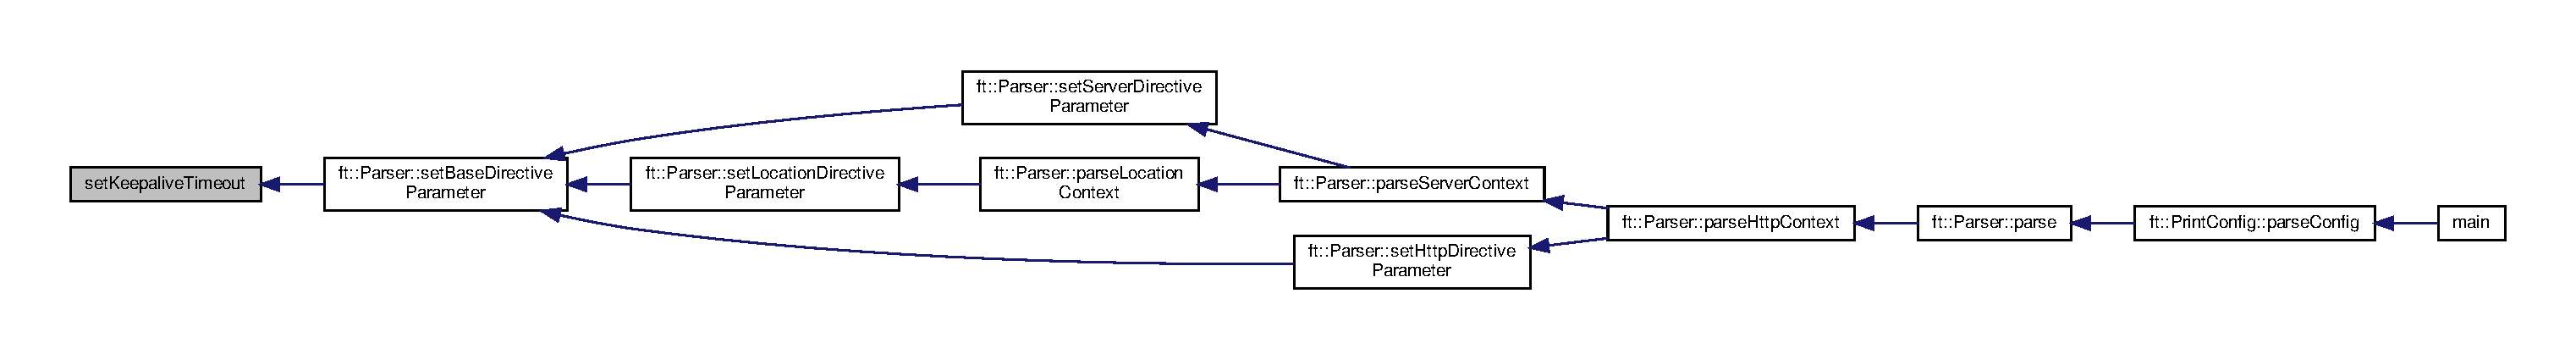
\includegraphics[width=350pt]{classft_1_1_base_directives_a0818b8529872ba9622329e2118d20c39_icgraph}
\end{center}
\end{figure}
\mbox{\Hypertarget{classft_1_1_base_directives_a2a7990e309f7e38f2915dbbb0d2704cf}\label{classft_1_1_base_directives_a2a7990e309f7e38f2915dbbb0d2704cf}} 
\index{ft\+::\+Http\+Block@{ft\+::\+Http\+Block}!set\+Root@{set\+Root}}
\index{set\+Root@{set\+Root}!ft\+::\+Http\+Block@{ft\+::\+Http\+Block}}
\subsubsection{\texorpdfstring{set\+Root()}{setRoot()}}
{\footnotesize\ttfamily void set\+Root (\begin{DoxyParamCaption}\item[{const std\+::string}]{x }\end{DoxyParamCaption})\hspace{0.3cm}{\ttfamily [inherited]}}



Definition at line 47 of file Base\+Directives.\+cpp.


\begin{DoxyCode}
48     \{
49         this->\hyperlink{classft_1_1_base_directives_abb1eaf0bba10b90172d6152e69457dc7}{root\_} = x;
50     \}
\end{DoxyCode}
Here is the caller graph for this function\+:\nopagebreak
\begin{figure}[H]
\begin{center}
\leavevmode
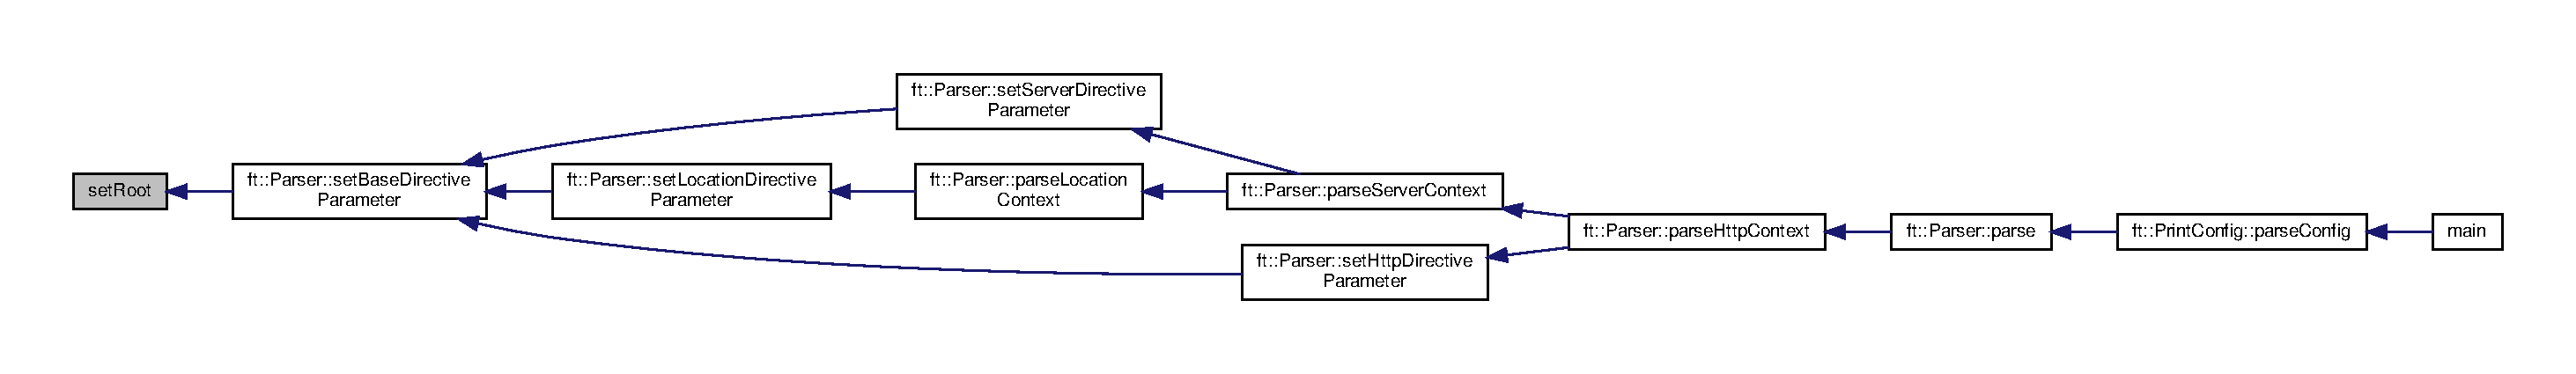
\includegraphics[width=350pt]{classft_1_1_base_directives_a2a7990e309f7e38f2915dbbb0d2704cf_icgraph}
\end{center}
\end{figure}


\subsection{Member Data Documentation}
\mbox{\Hypertarget{classft_1_1_base_directives_a4ebffbe32f50a462afa139c6f03c1a4f}\label{classft_1_1_base_directives_a4ebffbe32f50a462afa139c6f03c1a4f}} 
\index{ft\+::\+Http\+Block@{ft\+::\+Http\+Block}!autoindex\+\_\+@{autoindex\+\_\+}}
\index{autoindex\+\_\+@{autoindex\+\_\+}!ft\+::\+Http\+Block@{ft\+::\+Http\+Block}}
\subsubsection{\texorpdfstring{autoindex\+\_\+}{autoindex\_}}
{\footnotesize\ttfamily bool autoindex\+\_\+\hspace{0.3cm}{\ttfamily [protected]}, {\ttfamily [inherited]}}



Definition at line 16 of file Base\+Directives.\+hpp.

\mbox{\Hypertarget{classft_1_1_base_directives_ad65c2594d2a90ca065d410dfd4066a19}\label{classft_1_1_base_directives_ad65c2594d2a90ca065d410dfd4066a19}} 
\index{ft\+::\+Http\+Block@{ft\+::\+Http\+Block}!client\+Max\+Body\+Size\+\_\+@{client\+Max\+Body\+Size\+\_\+}}
\index{client\+Max\+Body\+Size\+\_\+@{client\+Max\+Body\+Size\+\_\+}!ft\+::\+Http\+Block@{ft\+::\+Http\+Block}}
\subsubsection{\texorpdfstring{client\+Max\+Body\+Size\+\_\+}{clientMaxBodySize\_}}
{\footnotesize\ttfamily unsigned long client\+Max\+Body\+Size\+\_\+\hspace{0.3cm}{\ttfamily [protected]}, {\ttfamily [inherited]}}



Definition at line 13 of file Base\+Directives.\+hpp.

\mbox{\Hypertarget{classft_1_1_base_directives_a5c0d388109f086503961de84fe3fce90}\label{classft_1_1_base_directives_a5c0d388109f086503961de84fe3fce90}} 
\index{ft\+::\+Http\+Block@{ft\+::\+Http\+Block}!error\+Page\+\_\+@{error\+Page\+\_\+}}
\index{error\+Page\+\_\+@{error\+Page\+\_\+}!ft\+::\+Http\+Block@{ft\+::\+Http\+Block}}
\subsubsection{\texorpdfstring{error\+Page\+\_\+}{errorPage\_}}
{\footnotesize\ttfamily std\+::string error\+Page\+\_\+\hspace{0.3cm}{\ttfamily [protected]}, {\ttfamily [inherited]}}



Definition at line 17 of file Base\+Directives.\+hpp.

\mbox{\Hypertarget{classft_1_1_base_directives_a6ba30626837f300201cd32c35d50aa49}\label{classft_1_1_base_directives_a6ba30626837f300201cd32c35d50aa49}} 
\index{ft\+::\+Http\+Block@{ft\+::\+Http\+Block}!index\+\_\+@{index\+\_\+}}
\index{index\+\_\+@{index\+\_\+}!ft\+::\+Http\+Block@{ft\+::\+Http\+Block}}
\subsubsection{\texorpdfstring{index\+\_\+}{index\_}}
{\footnotesize\ttfamily std\+::vector$<$std\+::string$>$ index\+\_\+\hspace{0.3cm}{\ttfamily [protected]}, {\ttfamily [inherited]}}



Definition at line 15 of file Base\+Directives.\+hpp.

\mbox{\Hypertarget{classft_1_1_base_directives_aa1f5f394b428d0d18765a9b9e14e648f}\label{classft_1_1_base_directives_aa1f5f394b428d0d18765a9b9e14e648f}} 
\index{ft\+::\+Http\+Block@{ft\+::\+Http\+Block}!keepalive\+Timeout\+\_\+@{keepalive\+Timeout\+\_\+}}
\index{keepalive\+Timeout\+\_\+@{keepalive\+Timeout\+\_\+}!ft\+::\+Http\+Block@{ft\+::\+Http\+Block}}
\subsubsection{\texorpdfstring{keepalive\+Timeout\+\_\+}{keepaliveTimeout\_}}
{\footnotesize\ttfamily unsigned int keepalive\+Timeout\+\_\+\hspace{0.3cm}{\ttfamily [protected]}, {\ttfamily [inherited]}}



Definition at line 14 of file Base\+Directives.\+hpp.

\mbox{\Hypertarget{classft_1_1_base_directives_abb1eaf0bba10b90172d6152e69457dc7}\label{classft_1_1_base_directives_abb1eaf0bba10b90172d6152e69457dc7}} 
\index{ft\+::\+Http\+Block@{ft\+::\+Http\+Block}!root\+\_\+@{root\+\_\+}}
\index{root\+\_\+@{root\+\_\+}!ft\+::\+Http\+Block@{ft\+::\+Http\+Block}}
\subsubsection{\texorpdfstring{root\+\_\+}{root\_}}
{\footnotesize\ttfamily std\+::string root\+\_\+\hspace{0.3cm}{\ttfamily [protected]}, {\ttfamily [inherited]}}



Definition at line 12 of file Base\+Directives.\+hpp.

\mbox{\Hypertarget{classft_1_1_http_block_ad832a81fa84d149a58e896f2036cd53b}\label{classft_1_1_http_block_ad832a81fa84d149a58e896f2036cd53b}} 
\index{ft\+::\+Http\+Block@{ft\+::\+Http\+Block}!server\+List@{server\+List}}
\index{server\+List@{server\+List}!ft\+::\+Http\+Block@{ft\+::\+Http\+Block}}
\subsubsection{\texorpdfstring{server\+List}{serverList}}
{\footnotesize\ttfamily std\+::vector$<$\hyperlink{classft_1_1_server_block}{Server\+Block}$>$ server\+List}



Definition at line 13 of file Http\+Block.\+hpp.



The documentation for this class was generated from the following files\+:\begin{DoxyCompactItemize}
\item 
/home/cjung-\/mo/\+Documents/42/\+Webserv/config/src/\hyperlink{_http_block_8hpp}{Http\+Block.\+hpp}\item 
/home/cjung-\/mo/\+Documents/42/\+Webserv/config/src/\hyperlink{_http_block_8cpp}{Http\+Block.\+cpp}\end{DoxyCompactItemize}

\hypertarget{classft_1_1_location_block}{}\section{Location\+Block Class Reference}
\label{classft_1_1_location_block}\index{Location\+Block@{Location\+Block}}


{\ttfamily \#include $<$Location\+Block.\+hpp$>$}



Inheritance diagram for Location\+Block\+:
\nopagebreak
\begin{figure}[H]
\begin{center}
\leavevmode
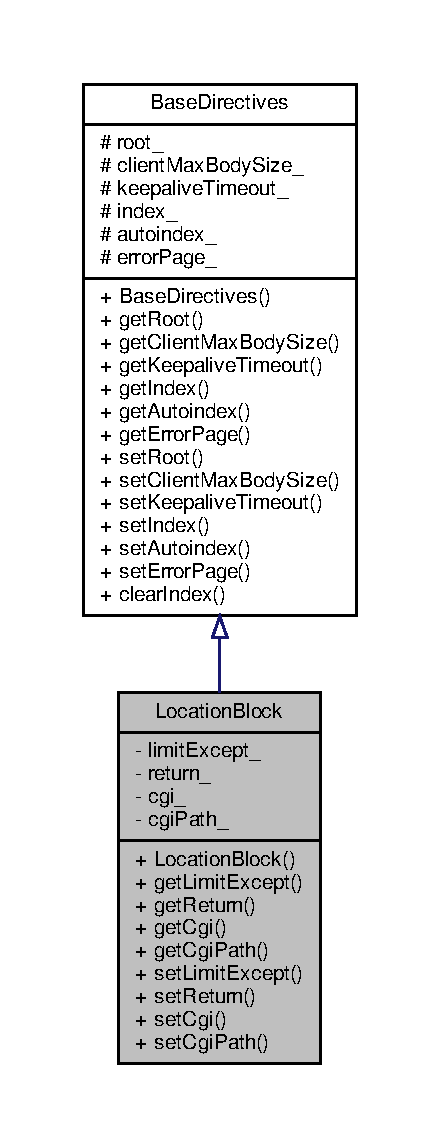
\includegraphics[height=550pt]{classft_1_1_location_block__inherit__graph}
\end{center}
\end{figure}


Collaboration diagram for Location\+Block\+:
\nopagebreak
\begin{figure}[H]
\begin{center}
\leavevmode
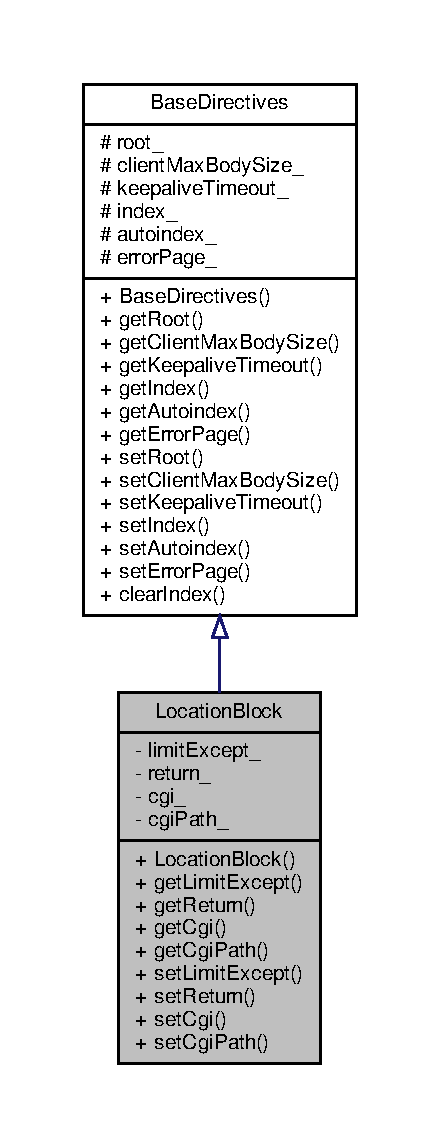
\includegraphics[height=550pt]{classft_1_1_location_block__coll__graph}
\end{center}
\end{figure}
\subsection*{Public Member Functions}
\begin{DoxyCompactItemize}
\item 
\hyperlink{classft_1_1_location_block_a28cbc9fd5dfde06685c8f7be5b6e0a4a}{Location\+Block} (const \hyperlink{classft_1_1_base_directives}{Base\+Directives} \&context)
\item 
const std\+::vector$<$ std\+::string $>$ \hyperlink{classft_1_1_location_block_ad2dc75d3f9c9f06f31e3948823557d52}{get\+Limit\+Except} (void) const
\item 
const std\+::vector$<$ std\+::string $>$ \hyperlink{classft_1_1_location_block_aeef5e4710c02406c46e54d4aa0c8f57c}{get\+Return} (void) const
\item 
const std\+::vector$<$ std\+::string $>$ \hyperlink{classft_1_1_location_block_adc8c829b27e09893233983eb1c727755}{get\+Cgi} (void) const
\item 
const std\+::string \hyperlink{classft_1_1_location_block_a9f90dac2d6314b77ccb9c9d4ab2a3fa4}{get\+Cgi\+Path} (void) const
\item 
void \hyperlink{classft_1_1_location_block_a307df676bb22688bb58396dd2c457848}{set\+Limit\+Except} (const std\+::string x)
\item 
void \hyperlink{classft_1_1_location_block_a041d07c701e052b114ef353d5e588998}{set\+Return} (const std\+::string x)
\item 
void \hyperlink{classft_1_1_location_block_a925a8d17e78d0cdea1b660e46e7be203}{set\+Cgi} (const std\+::string x)
\item 
void \hyperlink{classft_1_1_location_block_a25189c8c38f0b9ec831bb1b5295669c3}{set\+Cgi\+Path} (const std\+::string x)
\item 
const std\+::string \hyperlink{classft_1_1_base_directives_aa5dbcb08bda0a0e7e502d2df7cf64287}{get\+Root} (void) const
\item 
unsigned long \hyperlink{classft_1_1_base_directives_a930398ba1e4b99b2ba01a60dcda0c923}{get\+Client\+Max\+Body\+Size} (void) const
\item 
unsigned int \hyperlink{classft_1_1_base_directives_ab8574338758f65325cab5d1c394826c8}{get\+Keepalive\+Timeout} (void) const
\item 
const std\+::vector$<$ std\+::string $>$ \hyperlink{classft_1_1_base_directives_a018f34a5ffd66e891494b5c0ee69177b}{get\+Index} (void) const
\item 
bool \hyperlink{classft_1_1_base_directives_a4c11ed7ad76aeac228b029a2444de568}{get\+Autoindex} (void) const
\item 
const std\+::string \hyperlink{classft_1_1_base_directives_a3cb0c21f17781de392d5ee09d7190caf}{get\+Error\+Page} (void) const
\item 
void \hyperlink{classft_1_1_base_directives_a2a7990e309f7e38f2915dbbb0d2704cf}{set\+Root} (const std\+::string x)
\item 
void \hyperlink{classft_1_1_base_directives_a39bf4922f3236043c76beaffaa557a3b}{set\+Client\+Max\+Body\+Size} (const unsigned long x)
\item 
void \hyperlink{classft_1_1_base_directives_a0818b8529872ba9622329e2118d20c39}{set\+Keepalive\+Timeout} (const unsigned int x)
\item 
void \hyperlink{classft_1_1_base_directives_a6d3d8fd6eaaf71304128af6b3cee2a69}{set\+Index} (const std\+::string x)
\item 
void \hyperlink{classft_1_1_base_directives_ae7293c7bbf34e9bdc60c540dccd53342}{set\+Autoindex} (const bool x)
\item 
void \hyperlink{classft_1_1_base_directives_a505ecc88b3e1779583ad60cc243c7769}{set\+Error\+Page} (const std\+::string x)
\item 
void \hyperlink{classft_1_1_base_directives_a36d96dc74e650162c25a325813130ab2}{clear\+Index} (void)
\end{DoxyCompactItemize}
\subsection*{Protected Attributes}
\begin{DoxyCompactItemize}
\item 
std\+::string \hyperlink{classft_1_1_base_directives_abb1eaf0bba10b90172d6152e69457dc7}{root\+\_\+}
\item 
unsigned long \hyperlink{classft_1_1_base_directives_ad65c2594d2a90ca065d410dfd4066a19}{client\+Max\+Body\+Size\+\_\+}
\item 
unsigned int \hyperlink{classft_1_1_base_directives_aa1f5f394b428d0d18765a9b9e14e648f}{keepalive\+Timeout\+\_\+}
\item 
std\+::vector$<$ std\+::string $>$ \hyperlink{classft_1_1_base_directives_a6ba30626837f300201cd32c35d50aa49}{index\+\_\+}
\item 
bool \hyperlink{classft_1_1_base_directives_a4ebffbe32f50a462afa139c6f03c1a4f}{autoindex\+\_\+}
\item 
std\+::string \hyperlink{classft_1_1_base_directives_a5c0d388109f086503961de84fe3fce90}{error\+Page\+\_\+}
\end{DoxyCompactItemize}
\subsection*{Private Attributes}
\begin{DoxyCompactItemize}
\item 
std\+::vector$<$ std\+::string $>$ \hyperlink{classft_1_1_location_block_a8fec53119566b5654a7b902a1c53c6d9}{limit\+Except\+\_\+}
\item 
std\+::vector$<$ std\+::string $>$ \hyperlink{classft_1_1_location_block_abab721f365aff66f8a1289de21c8f01f}{return\+\_\+}
\item 
std\+::vector$<$ std\+::string $>$ \hyperlink{classft_1_1_location_block_a1952859864bec449ee1a20b4e90f829a}{cgi\+\_\+}
\item 
std\+::string \hyperlink{classft_1_1_location_block_a88189428cc92093d70626539b8851f5f}{cgi\+Path\+\_\+}
\end{DoxyCompactItemize}


\subsection{Detailed Description}


Definition at line 8 of file Location\+Block.\+hpp.



\subsection{Constructor \& Destructor Documentation}
\mbox{\Hypertarget{classft_1_1_location_block_a28cbc9fd5dfde06685c8f7be5b6e0a4a}\label{classft_1_1_location_block_a28cbc9fd5dfde06685c8f7be5b6e0a4a}} 
\index{ft\+::\+Location\+Block@{ft\+::\+Location\+Block}!Location\+Block@{Location\+Block}}
\index{Location\+Block@{Location\+Block}!ft\+::\+Location\+Block@{ft\+::\+Location\+Block}}
\subsubsection{\texorpdfstring{Location\+Block()}{LocationBlock()}}
{\footnotesize\ttfamily \hyperlink{classft_1_1_location_block}{Location\+Block} (\begin{DoxyParamCaption}\item[{const \hyperlink{classft_1_1_base_directives}{Base\+Directives} \&}]{context }\end{DoxyParamCaption})}



Definition at line 6 of file Location\+Block.\+cpp.


\begin{DoxyCode}
7     \{
8         this->\hyperlink{classft_1_1_base_directives_abb1eaf0bba10b90172d6152e69457dc7}{root\_} = context.getRoot();
9         this->\hyperlink{classft_1_1_base_directives_ad65c2594d2a90ca065d410dfd4066a19}{clientMaxBodySize\_} = context.getClientMaxBodySize();
10         this->\hyperlink{classft_1_1_base_directives_aa1f5f394b428d0d18765a9b9e14e648f}{keepaliveTimeout\_} = context.getKeepaliveTimeout();
11         this->\hyperlink{classft_1_1_base_directives_a6ba30626837f300201cd32c35d50aa49}{index\_} = context.getIndex();
12         this->\hyperlink{classft_1_1_base_directives_a4ebffbe32f50a462afa139c6f03c1a4f}{autoindex\_} = context.getAutoindex();
13         this->\hyperlink{classft_1_1_base_directives_a5c0d388109f086503961de84fe3fce90}{errorPage\_} = context.getErrorPage();
14     \}
\end{DoxyCode}
Here is the call graph for this function\+:\nopagebreak
\begin{figure}[H]
\begin{center}
\leavevmode
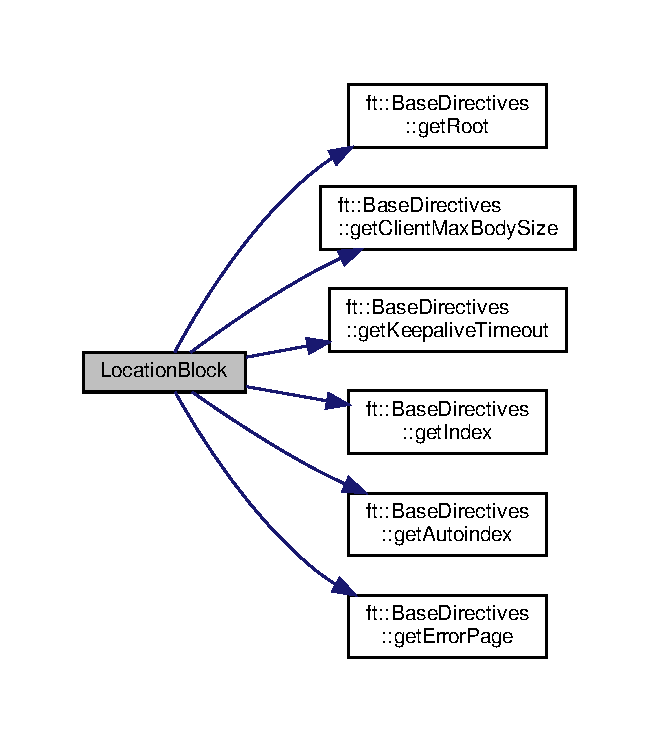
\includegraphics[width=316pt]{classft_1_1_location_block_a28cbc9fd5dfde06685c8f7be5b6e0a4a_cgraph}
\end{center}
\end{figure}


\subsection{Member Function Documentation}
\mbox{\Hypertarget{classft_1_1_base_directives_a36d96dc74e650162c25a325813130ab2}\label{classft_1_1_base_directives_a36d96dc74e650162c25a325813130ab2}} 
\index{ft\+::\+Location\+Block@{ft\+::\+Location\+Block}!clear\+Index@{clear\+Index}}
\index{clear\+Index@{clear\+Index}!ft\+::\+Location\+Block@{ft\+::\+Location\+Block}}
\subsubsection{\texorpdfstring{clear\+Index()}{clearIndex()}}
{\footnotesize\ttfamily void clear\+Index (\begin{DoxyParamCaption}\item[{void}]{ }\end{DoxyParamCaption})\hspace{0.3cm}{\ttfamily [inherited]}}



Definition at line 78 of file Base\+Directives.\+cpp.


\begin{DoxyCode}
79     \{
80         this->\hyperlink{classft_1_1_base_directives_a6ba30626837f300201cd32c35d50aa49}{index\_}.clear();
81     \}
\end{DoxyCode}
Here is the caller graph for this function\+:
\nopagebreak
\begin{figure}[H]
\begin{center}
\leavevmode
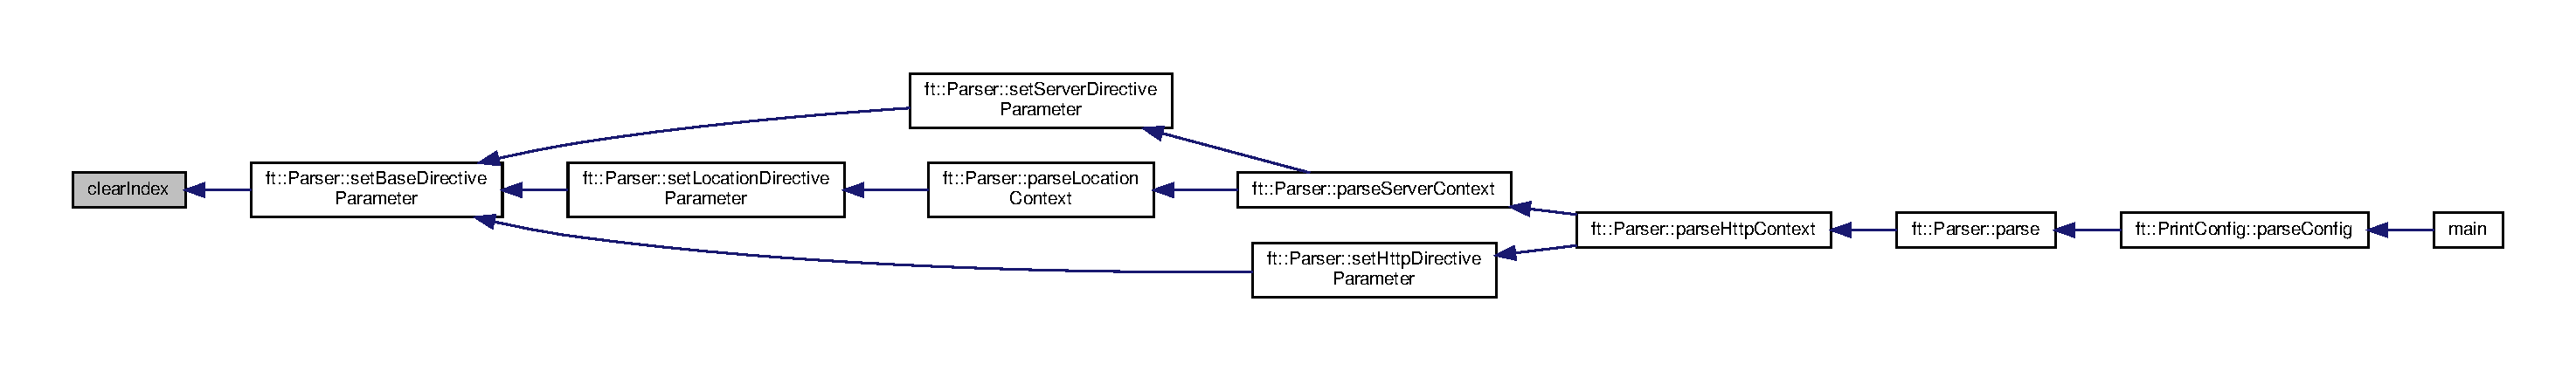
\includegraphics[width=350pt]{classft_1_1_base_directives_a36d96dc74e650162c25a325813130ab2_icgraph}
\end{center}
\end{figure}
\mbox{\Hypertarget{classft_1_1_base_directives_a4c11ed7ad76aeac228b029a2444de568}\label{classft_1_1_base_directives_a4c11ed7ad76aeac228b029a2444de568}} 
\index{ft\+::\+Location\+Block@{ft\+::\+Location\+Block}!get\+Autoindex@{get\+Autoindex}}
\index{get\+Autoindex@{get\+Autoindex}!ft\+::\+Location\+Block@{ft\+::\+Location\+Block}}
\subsubsection{\texorpdfstring{get\+Autoindex()}{getAutoindex()}}
{\footnotesize\ttfamily bool get\+Autoindex (\begin{DoxyParamCaption}\item[{void}]{ }\end{DoxyParamCaption}) const\hspace{0.3cm}{\ttfamily [inherited]}}



Definition at line 36 of file Base\+Directives.\+cpp.


\begin{DoxyCode}
37     \{
38         \textcolor{keywordflow}{return} (this->\hyperlink{classft_1_1_base_directives_a4ebffbe32f50a462afa139c6f03c1a4f}{autoindex\_});
39     \}
\end{DoxyCode}
Here is the caller graph for this function\+:
\nopagebreak
\begin{figure}[H]
\begin{center}
\leavevmode
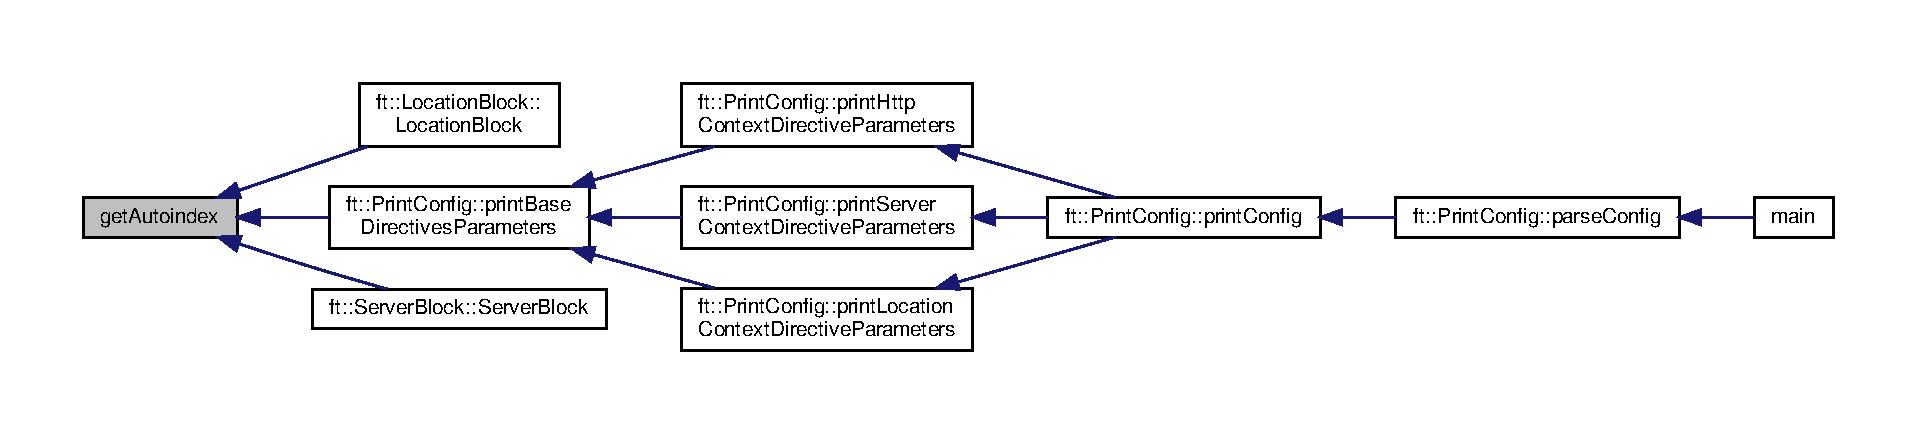
\includegraphics[width=350pt]{classft_1_1_base_directives_a4c11ed7ad76aeac228b029a2444de568_icgraph}
\end{center}
\end{figure}
\mbox{\Hypertarget{classft_1_1_location_block_adc8c829b27e09893233983eb1c727755}\label{classft_1_1_location_block_adc8c829b27e09893233983eb1c727755}} 
\index{ft\+::\+Location\+Block@{ft\+::\+Location\+Block}!get\+Cgi@{get\+Cgi}}
\index{get\+Cgi@{get\+Cgi}!ft\+::\+Location\+Block@{ft\+::\+Location\+Block}}
\subsubsection{\texorpdfstring{get\+Cgi()}{getCgi()}}
{\footnotesize\ttfamily const std\+::vector$<$ std\+::string $>$ get\+Cgi (\begin{DoxyParamCaption}\item[{void}]{ }\end{DoxyParamCaption}) const}



Definition at line 26 of file Location\+Block.\+cpp.


\begin{DoxyCode}
27     \{
28         \textcolor{keywordflow}{return} (this->\hyperlink{classft_1_1_location_block_a1952859864bec449ee1a20b4e90f829a}{cgi\_});
29     \}
\end{DoxyCode}
Here is the caller graph for this function\+:
\nopagebreak
\begin{figure}[H]
\begin{center}
\leavevmode
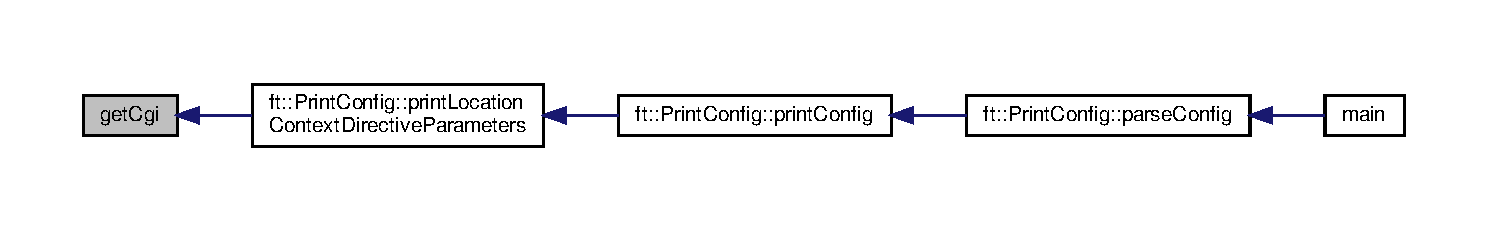
\includegraphics[width=350pt]{classft_1_1_location_block_adc8c829b27e09893233983eb1c727755_icgraph}
\end{center}
\end{figure}
\mbox{\Hypertarget{classft_1_1_location_block_a9f90dac2d6314b77ccb9c9d4ab2a3fa4}\label{classft_1_1_location_block_a9f90dac2d6314b77ccb9c9d4ab2a3fa4}} 
\index{ft\+::\+Location\+Block@{ft\+::\+Location\+Block}!get\+Cgi\+Path@{get\+Cgi\+Path}}
\index{get\+Cgi\+Path@{get\+Cgi\+Path}!ft\+::\+Location\+Block@{ft\+::\+Location\+Block}}
\subsubsection{\texorpdfstring{get\+Cgi\+Path()}{getCgiPath()}}
{\footnotesize\ttfamily const std\+::string get\+Cgi\+Path (\begin{DoxyParamCaption}\item[{void}]{ }\end{DoxyParamCaption}) const}



Definition at line 31 of file Location\+Block.\+cpp.


\begin{DoxyCode}
32     \{
33         \textcolor{keywordflow}{return} (this->\hyperlink{classft_1_1_location_block_a88189428cc92093d70626539b8851f5f}{cgiPath\_});
34     \}
\end{DoxyCode}
Here is the caller graph for this function\+:
\nopagebreak
\begin{figure}[H]
\begin{center}
\leavevmode
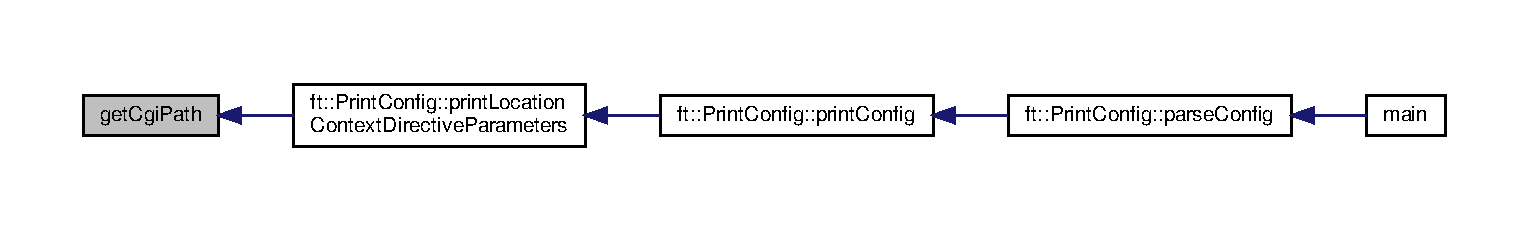
\includegraphics[width=350pt]{classft_1_1_location_block_a9f90dac2d6314b77ccb9c9d4ab2a3fa4_icgraph}
\end{center}
\end{figure}
\mbox{\Hypertarget{classft_1_1_base_directives_a930398ba1e4b99b2ba01a60dcda0c923}\label{classft_1_1_base_directives_a930398ba1e4b99b2ba01a60dcda0c923}} 
\index{ft\+::\+Location\+Block@{ft\+::\+Location\+Block}!get\+Client\+Max\+Body\+Size@{get\+Client\+Max\+Body\+Size}}
\index{get\+Client\+Max\+Body\+Size@{get\+Client\+Max\+Body\+Size}!ft\+::\+Location\+Block@{ft\+::\+Location\+Block}}
\subsubsection{\texorpdfstring{get\+Client\+Max\+Body\+Size()}{getClientMaxBodySize()}}
{\footnotesize\ttfamily unsigned long get\+Client\+Max\+Body\+Size (\begin{DoxyParamCaption}\item[{void}]{ }\end{DoxyParamCaption}) const\hspace{0.3cm}{\ttfamily [inherited]}}



Definition at line 21 of file Base\+Directives.\+cpp.


\begin{DoxyCode}
22     \{
23         \textcolor{keywordflow}{return} (this->\hyperlink{classft_1_1_base_directives_ad65c2594d2a90ca065d410dfd4066a19}{clientMaxBodySize\_});
24     \}
\end{DoxyCode}
Here is the caller graph for this function\+:
\nopagebreak
\begin{figure}[H]
\begin{center}
\leavevmode
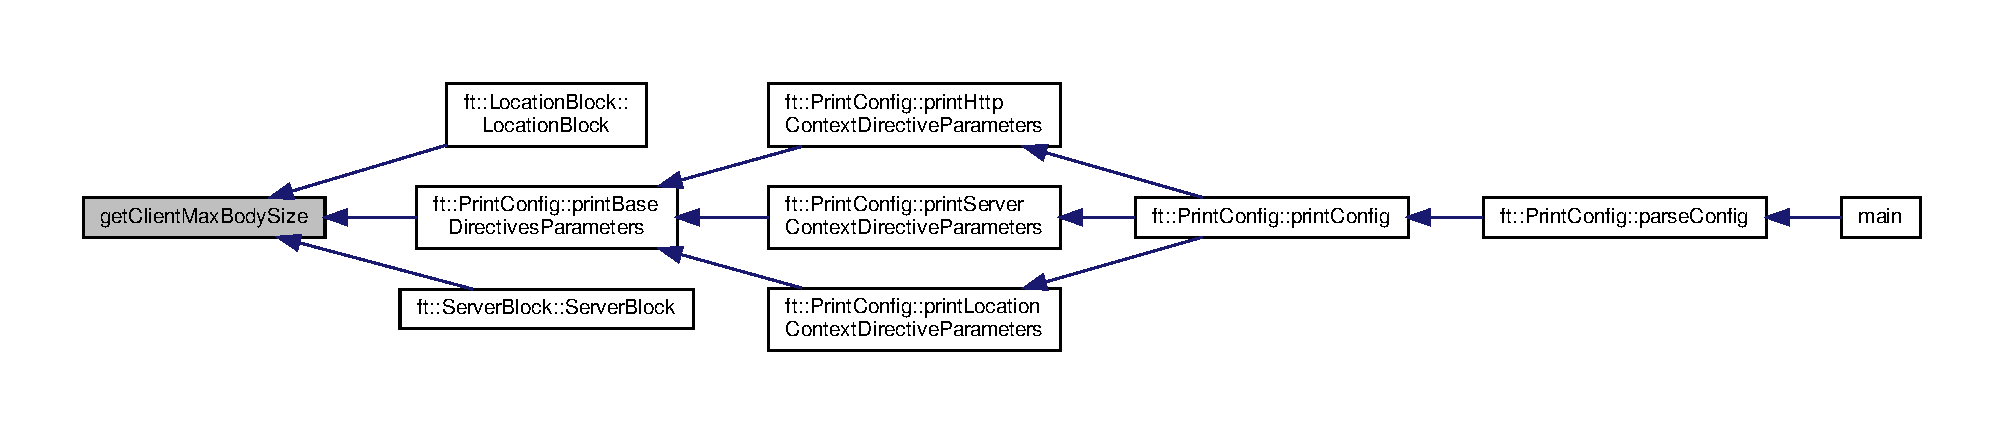
\includegraphics[width=350pt]{classft_1_1_base_directives_a930398ba1e4b99b2ba01a60dcda0c923_icgraph}
\end{center}
\end{figure}
\mbox{\Hypertarget{classft_1_1_base_directives_a3cb0c21f17781de392d5ee09d7190caf}\label{classft_1_1_base_directives_a3cb0c21f17781de392d5ee09d7190caf}} 
\index{ft\+::\+Location\+Block@{ft\+::\+Location\+Block}!get\+Error\+Page@{get\+Error\+Page}}
\index{get\+Error\+Page@{get\+Error\+Page}!ft\+::\+Location\+Block@{ft\+::\+Location\+Block}}
\subsubsection{\texorpdfstring{get\+Error\+Page()}{getErrorPage()}}
{\footnotesize\ttfamily const std\+::string get\+Error\+Page (\begin{DoxyParamCaption}\item[{void}]{ }\end{DoxyParamCaption}) const\hspace{0.3cm}{\ttfamily [inherited]}}



Definition at line 41 of file Base\+Directives.\+cpp.


\begin{DoxyCode}
42     \{
43         \textcolor{keywordflow}{return} (this->\hyperlink{classft_1_1_base_directives_a5c0d388109f086503961de84fe3fce90}{errorPage\_});
44     \}
\end{DoxyCode}
Here is the caller graph for this function\+:
\nopagebreak
\begin{figure}[H]
\begin{center}
\leavevmode
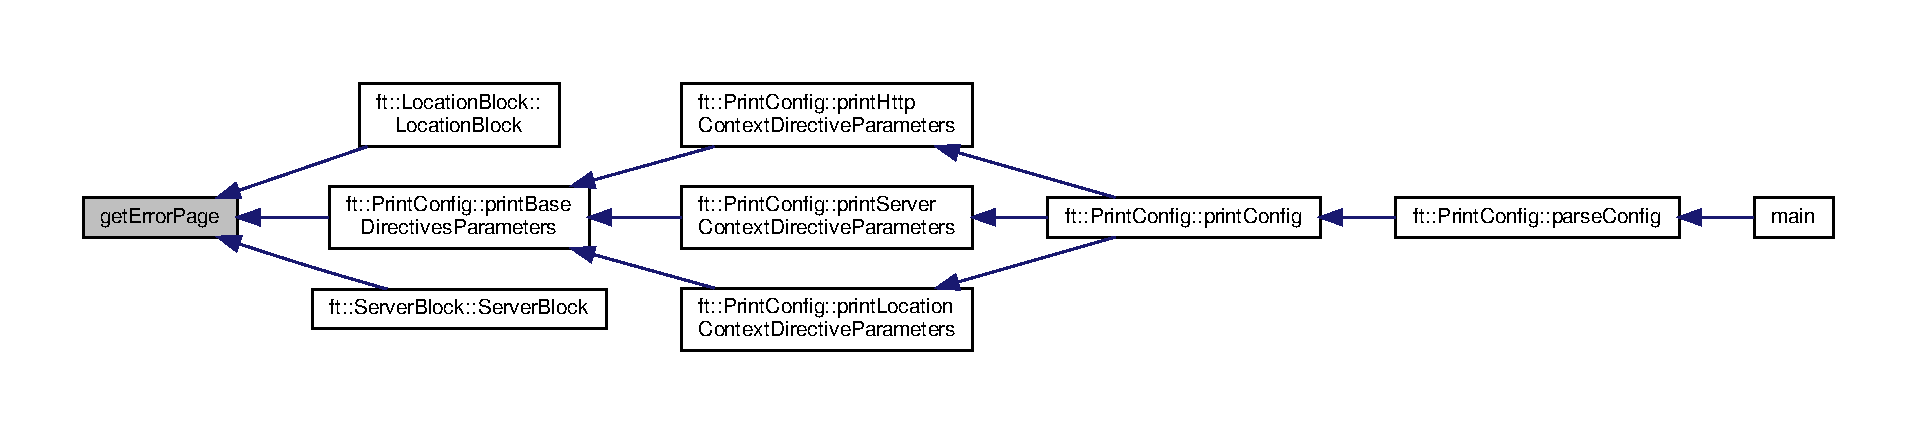
\includegraphics[width=350pt]{classft_1_1_base_directives_a3cb0c21f17781de392d5ee09d7190caf_icgraph}
\end{center}
\end{figure}
\mbox{\Hypertarget{classft_1_1_base_directives_a018f34a5ffd66e891494b5c0ee69177b}\label{classft_1_1_base_directives_a018f34a5ffd66e891494b5c0ee69177b}} 
\index{ft\+::\+Location\+Block@{ft\+::\+Location\+Block}!get\+Index@{get\+Index}}
\index{get\+Index@{get\+Index}!ft\+::\+Location\+Block@{ft\+::\+Location\+Block}}
\subsubsection{\texorpdfstring{get\+Index()}{getIndex()}}
{\footnotesize\ttfamily const std\+::vector$<$ std\+::string $>$ get\+Index (\begin{DoxyParamCaption}\item[{void}]{ }\end{DoxyParamCaption}) const\hspace{0.3cm}{\ttfamily [inherited]}}



Definition at line 31 of file Base\+Directives.\+cpp.


\begin{DoxyCode}
32     \{
33         \textcolor{keywordflow}{return} (this->\hyperlink{classft_1_1_base_directives_a6ba30626837f300201cd32c35d50aa49}{index\_});
34     \}
\end{DoxyCode}
Here is the caller graph for this function\+:
\nopagebreak
\begin{figure}[H]
\begin{center}
\leavevmode
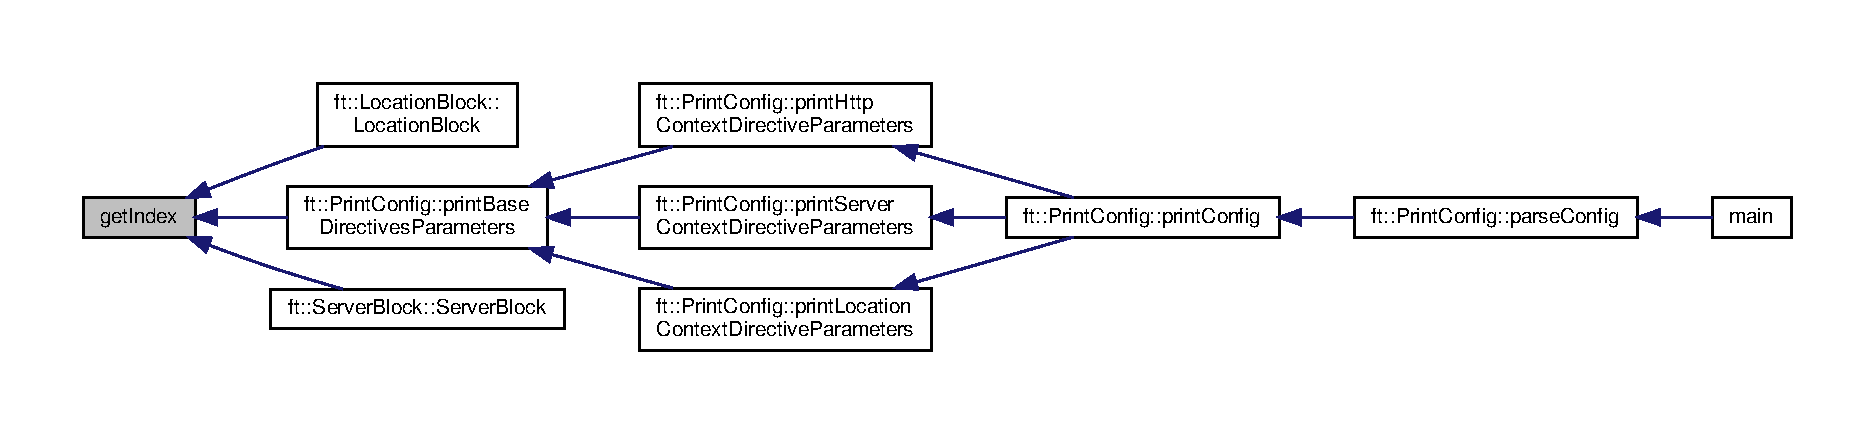
\includegraphics[width=350pt]{classft_1_1_base_directives_a018f34a5ffd66e891494b5c0ee69177b_icgraph}
\end{center}
\end{figure}
\mbox{\Hypertarget{classft_1_1_base_directives_ab8574338758f65325cab5d1c394826c8}\label{classft_1_1_base_directives_ab8574338758f65325cab5d1c394826c8}} 
\index{ft\+::\+Location\+Block@{ft\+::\+Location\+Block}!get\+Keepalive\+Timeout@{get\+Keepalive\+Timeout}}
\index{get\+Keepalive\+Timeout@{get\+Keepalive\+Timeout}!ft\+::\+Location\+Block@{ft\+::\+Location\+Block}}
\subsubsection{\texorpdfstring{get\+Keepalive\+Timeout()}{getKeepaliveTimeout()}}
{\footnotesize\ttfamily unsigned int get\+Keepalive\+Timeout (\begin{DoxyParamCaption}\item[{void}]{ }\end{DoxyParamCaption}) const\hspace{0.3cm}{\ttfamily [inherited]}}



Definition at line 26 of file Base\+Directives.\+cpp.


\begin{DoxyCode}
27     \{
28         \textcolor{keywordflow}{return} (this->\hyperlink{classft_1_1_base_directives_aa1f5f394b428d0d18765a9b9e14e648f}{keepaliveTimeout\_});
29     \}
\end{DoxyCode}
Here is the caller graph for this function\+:
\nopagebreak
\begin{figure}[H]
\begin{center}
\leavevmode
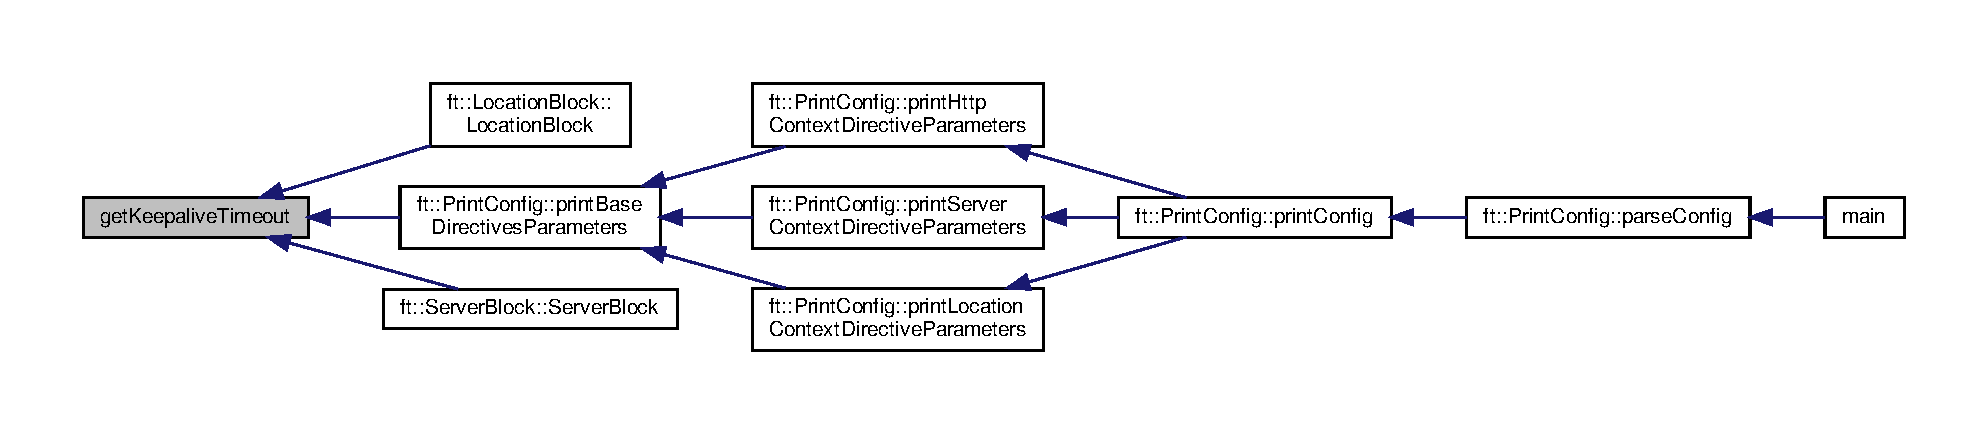
\includegraphics[width=350pt]{classft_1_1_base_directives_ab8574338758f65325cab5d1c394826c8_icgraph}
\end{center}
\end{figure}
\mbox{\Hypertarget{classft_1_1_location_block_ad2dc75d3f9c9f06f31e3948823557d52}\label{classft_1_1_location_block_ad2dc75d3f9c9f06f31e3948823557d52}} 
\index{ft\+::\+Location\+Block@{ft\+::\+Location\+Block}!get\+Limit\+Except@{get\+Limit\+Except}}
\index{get\+Limit\+Except@{get\+Limit\+Except}!ft\+::\+Location\+Block@{ft\+::\+Location\+Block}}
\subsubsection{\texorpdfstring{get\+Limit\+Except()}{getLimitExcept()}}
{\footnotesize\ttfamily const std\+::vector$<$ std\+::string $>$ get\+Limit\+Except (\begin{DoxyParamCaption}\item[{void}]{ }\end{DoxyParamCaption}) const}



Definition at line 17 of file Location\+Block.\+cpp.


\begin{DoxyCode}
18     \{
19         \textcolor{keywordflow}{return} (this->\hyperlink{classft_1_1_location_block_a8fec53119566b5654a7b902a1c53c6d9}{limitExcept\_});
20     \}
\end{DoxyCode}
Here is the caller graph for this function\+:
\nopagebreak
\begin{figure}[H]
\begin{center}
\leavevmode
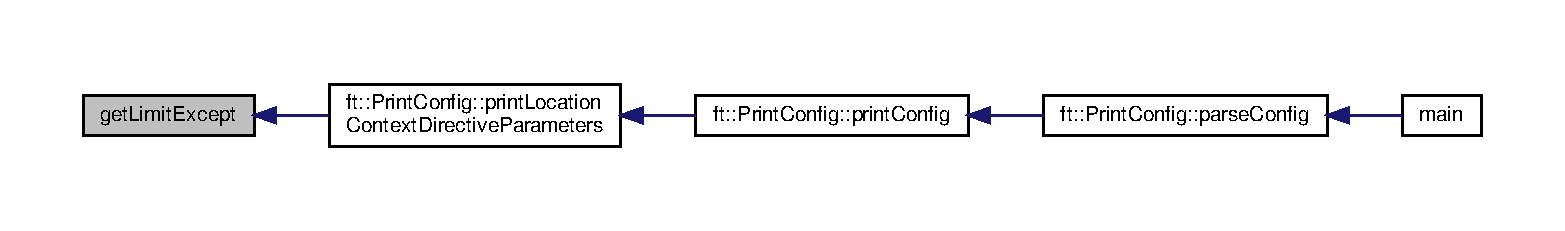
\includegraphics[width=350pt]{classft_1_1_location_block_ad2dc75d3f9c9f06f31e3948823557d52_icgraph}
\end{center}
\end{figure}
\mbox{\Hypertarget{classft_1_1_location_block_aeef5e4710c02406c46e54d4aa0c8f57c}\label{classft_1_1_location_block_aeef5e4710c02406c46e54d4aa0c8f57c}} 
\index{ft\+::\+Location\+Block@{ft\+::\+Location\+Block}!get\+Return@{get\+Return}}
\index{get\+Return@{get\+Return}!ft\+::\+Location\+Block@{ft\+::\+Location\+Block}}
\subsubsection{\texorpdfstring{get\+Return()}{getReturn()}}
{\footnotesize\ttfamily const std\+::vector$<$ std\+::string $>$ get\+Return (\begin{DoxyParamCaption}\item[{void}]{ }\end{DoxyParamCaption}) const}



Definition at line 22 of file Location\+Block.\+cpp.


\begin{DoxyCode}
23     \{
24         \textcolor{keywordflow}{return} (this->\hyperlink{classft_1_1_location_block_abab721f365aff66f8a1289de21c8f01f}{return\_});
25     \}
\end{DoxyCode}
Here is the caller graph for this function\+:
\nopagebreak
\begin{figure}[H]
\begin{center}
\leavevmode
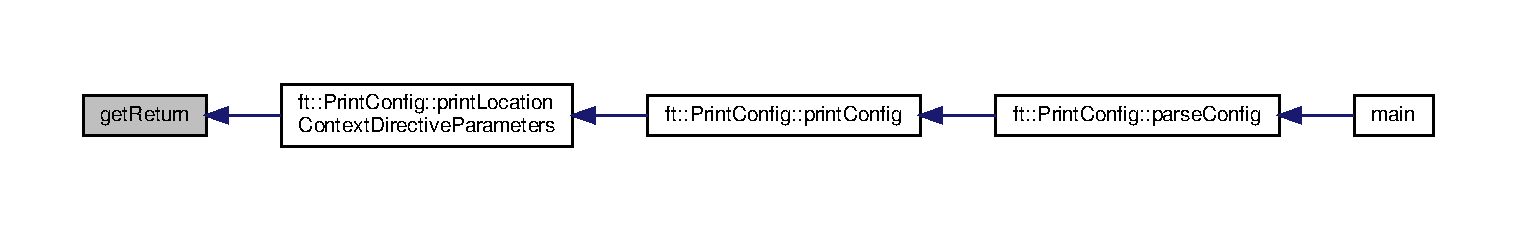
\includegraphics[width=350pt]{classft_1_1_location_block_aeef5e4710c02406c46e54d4aa0c8f57c_icgraph}
\end{center}
\end{figure}
\mbox{\Hypertarget{classft_1_1_base_directives_aa5dbcb08bda0a0e7e502d2df7cf64287}\label{classft_1_1_base_directives_aa5dbcb08bda0a0e7e502d2df7cf64287}} 
\index{ft\+::\+Location\+Block@{ft\+::\+Location\+Block}!get\+Root@{get\+Root}}
\index{get\+Root@{get\+Root}!ft\+::\+Location\+Block@{ft\+::\+Location\+Block}}
\subsubsection{\texorpdfstring{get\+Root()}{getRoot()}}
{\footnotesize\ttfamily const std\+::string get\+Root (\begin{DoxyParamCaption}\item[{void}]{ }\end{DoxyParamCaption}) const\hspace{0.3cm}{\ttfamily [inherited]}}



Definition at line 16 of file Base\+Directives.\+cpp.


\begin{DoxyCode}
17     \{
18         \textcolor{keywordflow}{return} (this->\hyperlink{classft_1_1_base_directives_abb1eaf0bba10b90172d6152e69457dc7}{root\_});
19     \}
\end{DoxyCode}
Here is the caller graph for this function\+:
\nopagebreak
\begin{figure}[H]
\begin{center}
\leavevmode
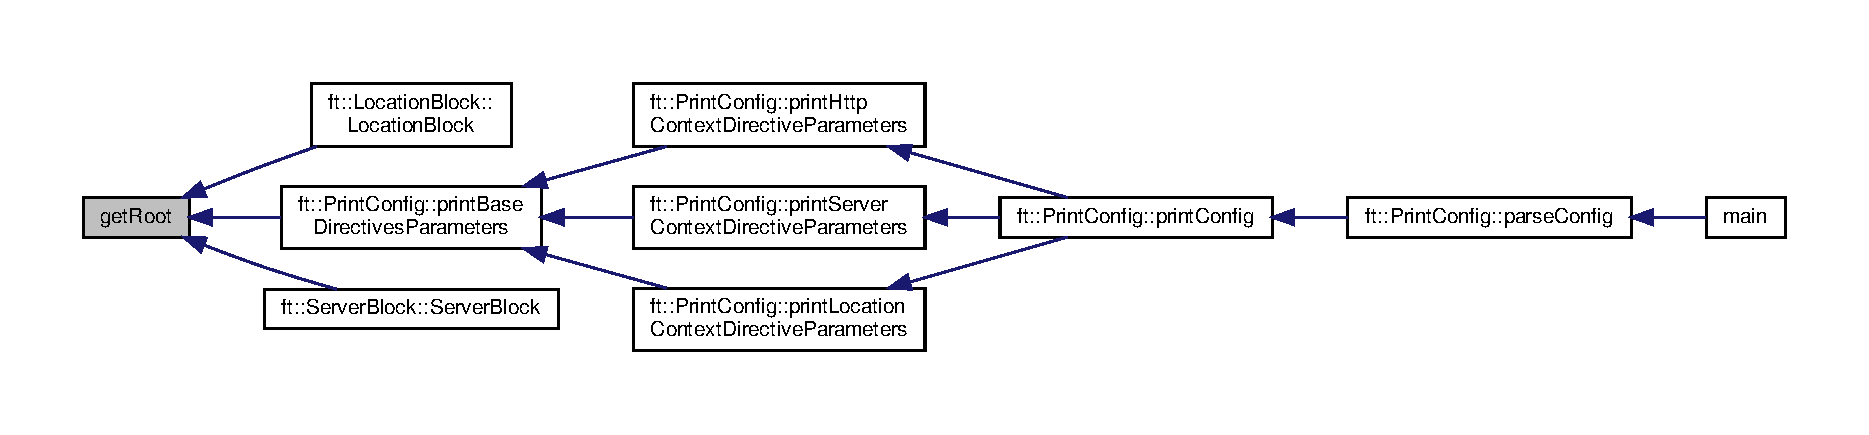
\includegraphics[width=350pt]{classft_1_1_base_directives_aa5dbcb08bda0a0e7e502d2df7cf64287_icgraph}
\end{center}
\end{figure}
\mbox{\Hypertarget{classft_1_1_base_directives_ae7293c7bbf34e9bdc60c540dccd53342}\label{classft_1_1_base_directives_ae7293c7bbf34e9bdc60c540dccd53342}} 
\index{ft\+::\+Location\+Block@{ft\+::\+Location\+Block}!set\+Autoindex@{set\+Autoindex}}
\index{set\+Autoindex@{set\+Autoindex}!ft\+::\+Location\+Block@{ft\+::\+Location\+Block}}
\subsubsection{\texorpdfstring{set\+Autoindex()}{setAutoindex()}}
{\footnotesize\ttfamily void set\+Autoindex (\begin{DoxyParamCaption}\item[{const bool}]{x }\end{DoxyParamCaption})\hspace{0.3cm}{\ttfamily [inherited]}}



Definition at line 67 of file Base\+Directives.\+cpp.


\begin{DoxyCode}
68     \{
69         this->\hyperlink{classft_1_1_base_directives_a4ebffbe32f50a462afa139c6f03c1a4f}{autoindex\_} = x;
70     \}
\end{DoxyCode}
Here is the caller graph for this function\+:
\nopagebreak
\begin{figure}[H]
\begin{center}
\leavevmode
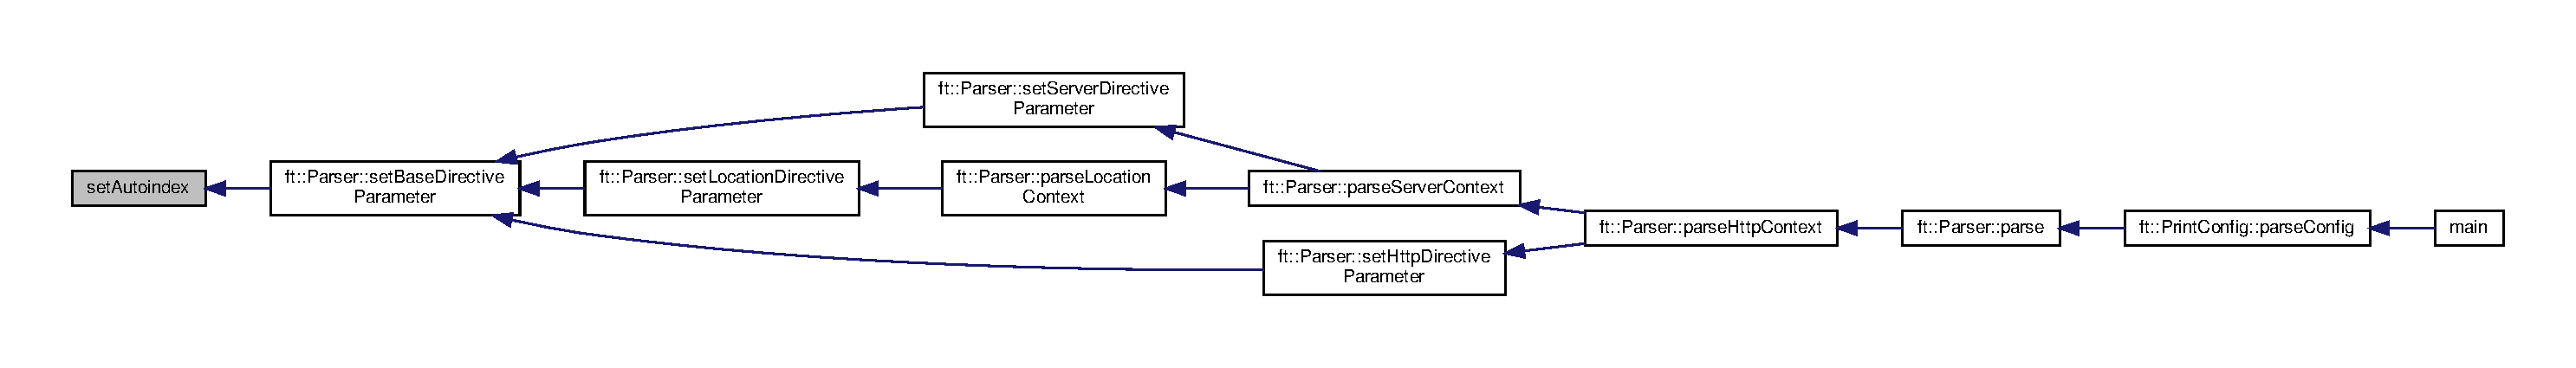
\includegraphics[width=350pt]{classft_1_1_base_directives_ae7293c7bbf34e9bdc60c540dccd53342_icgraph}
\end{center}
\end{figure}
\mbox{\Hypertarget{classft_1_1_location_block_a925a8d17e78d0cdea1b660e46e7be203}\label{classft_1_1_location_block_a925a8d17e78d0cdea1b660e46e7be203}} 
\index{ft\+::\+Location\+Block@{ft\+::\+Location\+Block}!set\+Cgi@{set\+Cgi}}
\index{set\+Cgi@{set\+Cgi}!ft\+::\+Location\+Block@{ft\+::\+Location\+Block}}
\subsubsection{\texorpdfstring{set\+Cgi()}{setCgi()}}
{\footnotesize\ttfamily void set\+Cgi (\begin{DoxyParamCaption}\item[{const std\+::string}]{x }\end{DoxyParamCaption})}



Definition at line 46 of file Location\+Block.\+cpp.


\begin{DoxyCode}
47     \{
48         this->\hyperlink{classft_1_1_location_block_a1952859864bec449ee1a20b4e90f829a}{cgi\_}.push\_back(x);
49     \}
\end{DoxyCode}
Here is the caller graph for this function\+:
\nopagebreak
\begin{figure}[H]
\begin{center}
\leavevmode
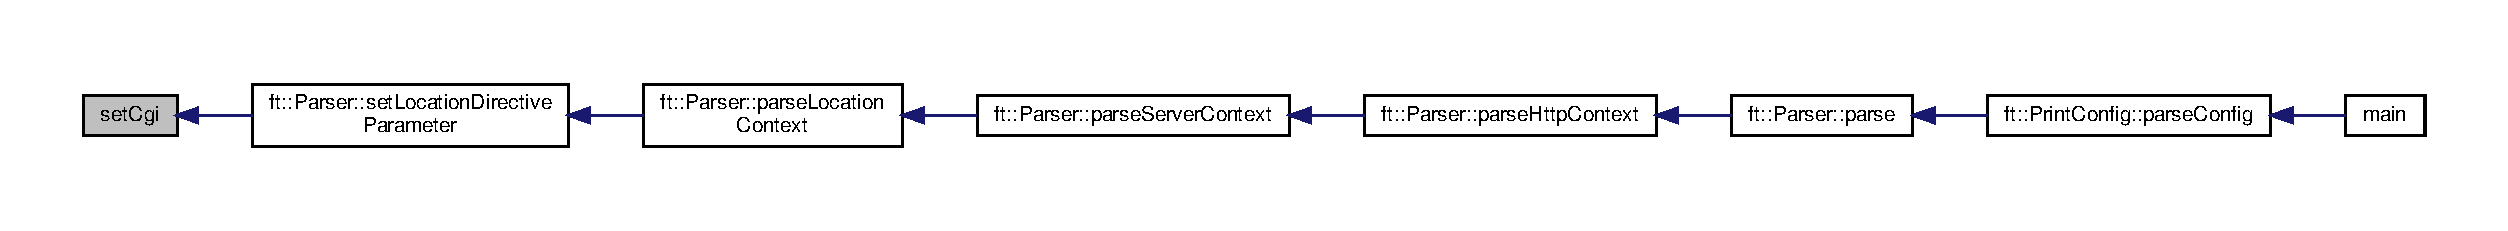
\includegraphics[width=350pt]{classft_1_1_location_block_a925a8d17e78d0cdea1b660e46e7be203_icgraph}
\end{center}
\end{figure}
\mbox{\Hypertarget{classft_1_1_location_block_a25189c8c38f0b9ec831bb1b5295669c3}\label{classft_1_1_location_block_a25189c8c38f0b9ec831bb1b5295669c3}} 
\index{ft\+::\+Location\+Block@{ft\+::\+Location\+Block}!set\+Cgi\+Path@{set\+Cgi\+Path}}
\index{set\+Cgi\+Path@{set\+Cgi\+Path}!ft\+::\+Location\+Block@{ft\+::\+Location\+Block}}
\subsubsection{\texorpdfstring{set\+Cgi\+Path()}{setCgiPath()}}
{\footnotesize\ttfamily void set\+Cgi\+Path (\begin{DoxyParamCaption}\item[{const std\+::string}]{x }\end{DoxyParamCaption})}



Definition at line 51 of file Location\+Block.\+cpp.


\begin{DoxyCode}
52     \{
53         this->\hyperlink{classft_1_1_location_block_a88189428cc92093d70626539b8851f5f}{cgiPath\_} = x;
54     \}
\end{DoxyCode}
Here is the caller graph for this function\+:
\nopagebreak
\begin{figure}[H]
\begin{center}
\leavevmode
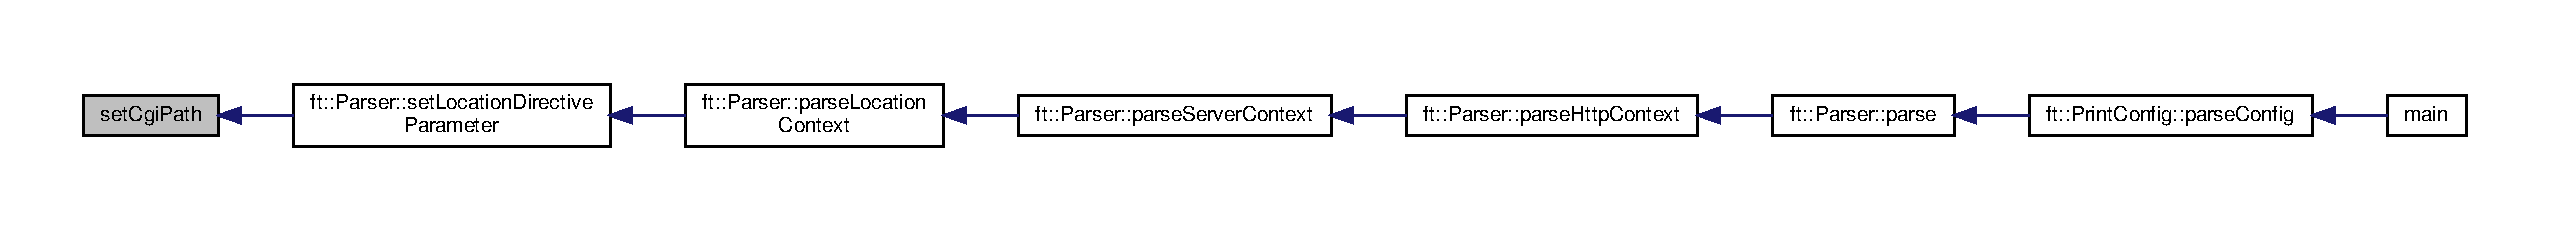
\includegraphics[width=350pt]{classft_1_1_location_block_a25189c8c38f0b9ec831bb1b5295669c3_icgraph}
\end{center}
\end{figure}
\mbox{\Hypertarget{classft_1_1_base_directives_a39bf4922f3236043c76beaffaa557a3b}\label{classft_1_1_base_directives_a39bf4922f3236043c76beaffaa557a3b}} 
\index{ft\+::\+Location\+Block@{ft\+::\+Location\+Block}!set\+Client\+Max\+Body\+Size@{set\+Client\+Max\+Body\+Size}}
\index{set\+Client\+Max\+Body\+Size@{set\+Client\+Max\+Body\+Size}!ft\+::\+Location\+Block@{ft\+::\+Location\+Block}}
\subsubsection{\texorpdfstring{set\+Client\+Max\+Body\+Size()}{setClientMaxBodySize()}}
{\footnotesize\ttfamily void set\+Client\+Max\+Body\+Size (\begin{DoxyParamCaption}\item[{const unsigned long}]{x }\end{DoxyParamCaption})\hspace{0.3cm}{\ttfamily [inherited]}}



Definition at line 52 of file Base\+Directives.\+cpp.


\begin{DoxyCode}
53     \{
54         this->\hyperlink{classft_1_1_base_directives_ad65c2594d2a90ca065d410dfd4066a19}{clientMaxBodySize\_} = x;
55     \}
\end{DoxyCode}
Here is the caller graph for this function\+:
\nopagebreak
\begin{figure}[H]
\begin{center}
\leavevmode
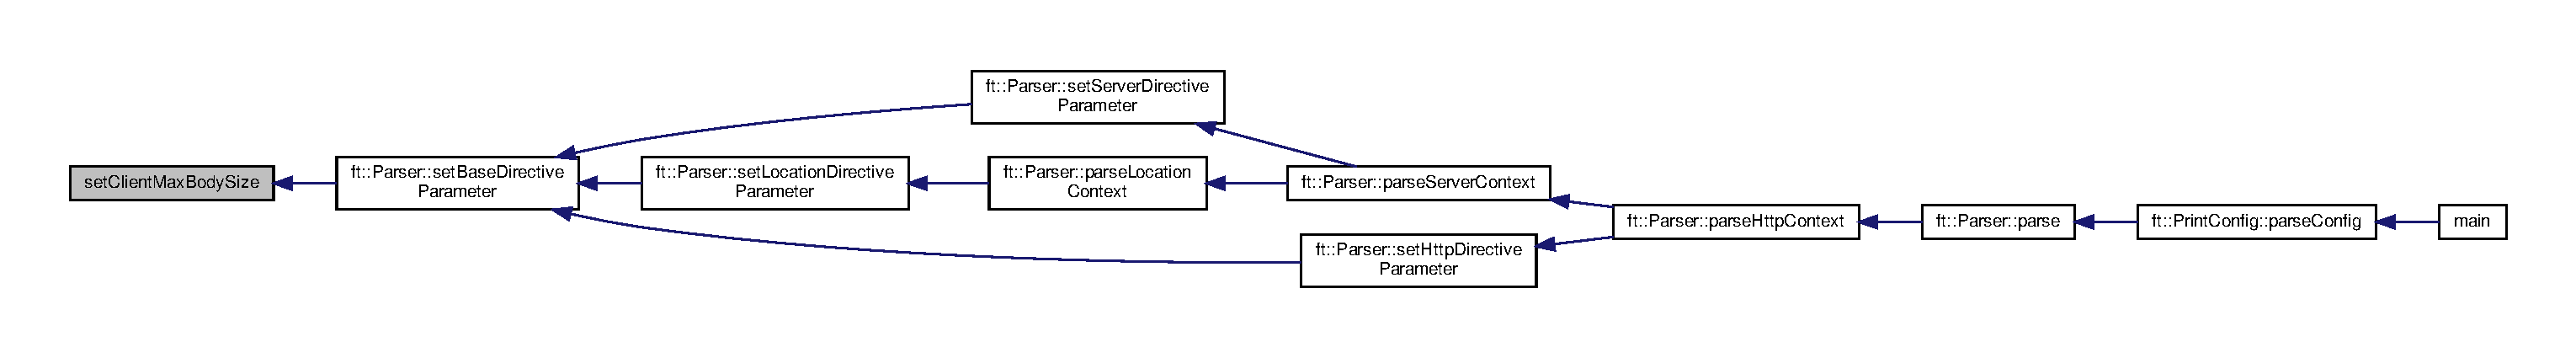
\includegraphics[width=350pt]{classft_1_1_base_directives_a39bf4922f3236043c76beaffaa557a3b_icgraph}
\end{center}
\end{figure}
\mbox{\Hypertarget{classft_1_1_base_directives_a505ecc88b3e1779583ad60cc243c7769}\label{classft_1_1_base_directives_a505ecc88b3e1779583ad60cc243c7769}} 
\index{ft\+::\+Location\+Block@{ft\+::\+Location\+Block}!set\+Error\+Page@{set\+Error\+Page}}
\index{set\+Error\+Page@{set\+Error\+Page}!ft\+::\+Location\+Block@{ft\+::\+Location\+Block}}
\subsubsection{\texorpdfstring{set\+Error\+Page()}{setErrorPage()}}
{\footnotesize\ttfamily void set\+Error\+Page (\begin{DoxyParamCaption}\item[{const std\+::string}]{x }\end{DoxyParamCaption})\hspace{0.3cm}{\ttfamily [inherited]}}



Definition at line 72 of file Base\+Directives.\+cpp.


\begin{DoxyCode}
73     \{
74         this->\hyperlink{classft_1_1_base_directives_a5c0d388109f086503961de84fe3fce90}{errorPage\_} = x;
75     \}
\end{DoxyCode}
Here is the caller graph for this function\+:
\nopagebreak
\begin{figure}[H]
\begin{center}
\leavevmode
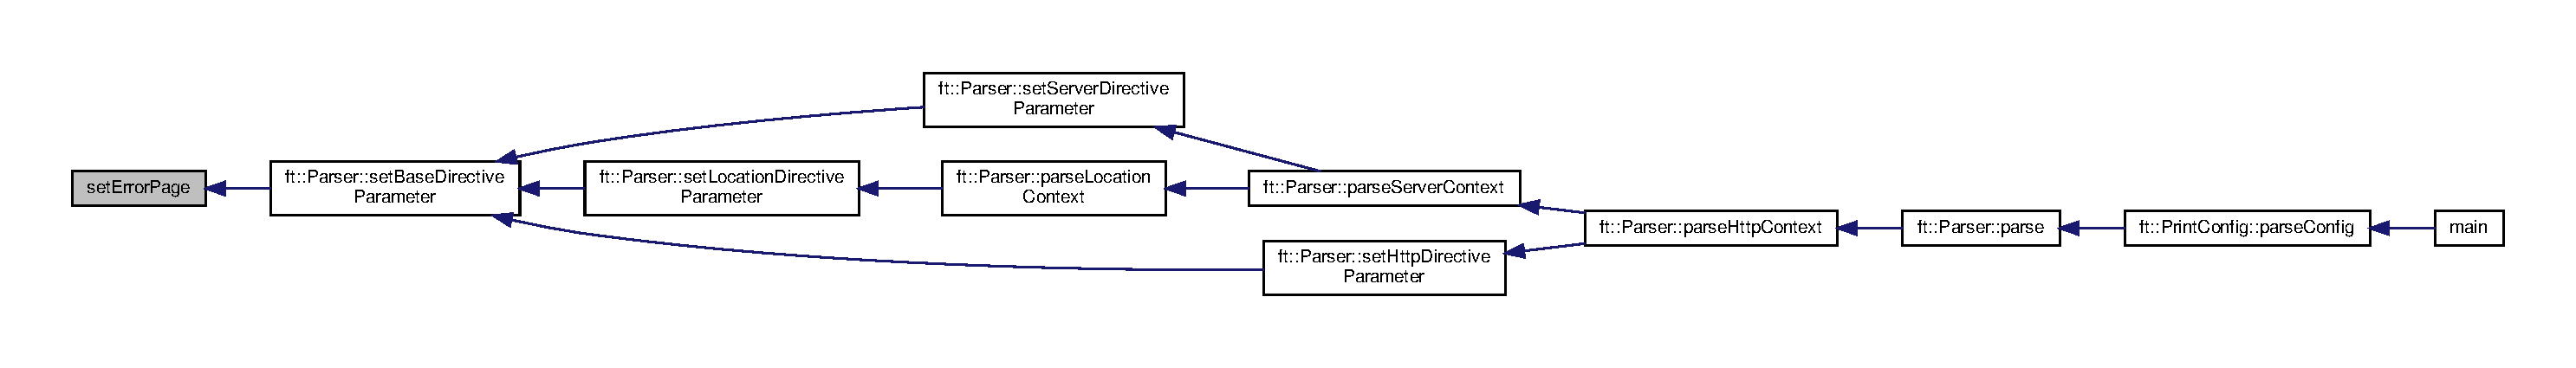
\includegraphics[width=350pt]{classft_1_1_base_directives_a505ecc88b3e1779583ad60cc243c7769_icgraph}
\end{center}
\end{figure}
\mbox{\Hypertarget{classft_1_1_base_directives_a6d3d8fd6eaaf71304128af6b3cee2a69}\label{classft_1_1_base_directives_a6d3d8fd6eaaf71304128af6b3cee2a69}} 
\index{ft\+::\+Location\+Block@{ft\+::\+Location\+Block}!set\+Index@{set\+Index}}
\index{set\+Index@{set\+Index}!ft\+::\+Location\+Block@{ft\+::\+Location\+Block}}
\subsubsection{\texorpdfstring{set\+Index()}{setIndex()}}
{\footnotesize\ttfamily void set\+Index (\begin{DoxyParamCaption}\item[{const std\+::string}]{x }\end{DoxyParamCaption})\hspace{0.3cm}{\ttfamily [inherited]}}



Definition at line 62 of file Base\+Directives.\+cpp.


\begin{DoxyCode}
63     \{
64         this->\hyperlink{classft_1_1_base_directives_a6ba30626837f300201cd32c35d50aa49}{index\_}.push\_back(x);
65     \}
\end{DoxyCode}
Here is the caller graph for this function\+:
\nopagebreak
\begin{figure}[H]
\begin{center}
\leavevmode
\includegraphics[width=350pt]{classft_1_1_base_directives_a6d3d8fd6eaaf71304128af6b3cee2a69_icgraph}
\end{center}
\end{figure}
\mbox{\Hypertarget{classft_1_1_base_directives_a0818b8529872ba9622329e2118d20c39}\label{classft_1_1_base_directives_a0818b8529872ba9622329e2118d20c39}} 
\index{ft\+::\+Location\+Block@{ft\+::\+Location\+Block}!set\+Keepalive\+Timeout@{set\+Keepalive\+Timeout}}
\index{set\+Keepalive\+Timeout@{set\+Keepalive\+Timeout}!ft\+::\+Location\+Block@{ft\+::\+Location\+Block}}
\subsubsection{\texorpdfstring{set\+Keepalive\+Timeout()}{setKeepaliveTimeout()}}
{\footnotesize\ttfamily void set\+Keepalive\+Timeout (\begin{DoxyParamCaption}\item[{const unsigned int}]{x }\end{DoxyParamCaption})\hspace{0.3cm}{\ttfamily [inherited]}}



Definition at line 57 of file Base\+Directives.\+cpp.


\begin{DoxyCode}
58     \{
59         this->\hyperlink{classft_1_1_base_directives_aa1f5f394b428d0d18765a9b9e14e648f}{keepaliveTimeout\_} = x;
60     \}
\end{DoxyCode}
Here is the caller graph for this function\+:
\nopagebreak
\begin{figure}[H]
\begin{center}
\leavevmode
\includegraphics[width=350pt]{classft_1_1_base_directives_a0818b8529872ba9622329e2118d20c39_icgraph}
\end{center}
\end{figure}
\mbox{\Hypertarget{classft_1_1_location_block_a307df676bb22688bb58396dd2c457848}\label{classft_1_1_location_block_a307df676bb22688bb58396dd2c457848}} 
\index{ft\+::\+Location\+Block@{ft\+::\+Location\+Block}!set\+Limit\+Except@{set\+Limit\+Except}}
\index{set\+Limit\+Except@{set\+Limit\+Except}!ft\+::\+Location\+Block@{ft\+::\+Location\+Block}}
\subsubsection{\texorpdfstring{set\+Limit\+Except()}{setLimitExcept()}}
{\footnotesize\ttfamily void set\+Limit\+Except (\begin{DoxyParamCaption}\item[{const std\+::string}]{x }\end{DoxyParamCaption})}



Definition at line 37 of file Location\+Block.\+cpp.


\begin{DoxyCode}
38     \{
39         this->\hyperlink{classft_1_1_location_block_a8fec53119566b5654a7b902a1c53c6d9}{limitExcept\_}.push\_back(x);
40     \}
\end{DoxyCode}
Here is the caller graph for this function\+:
\nopagebreak
\begin{figure}[H]
\begin{center}
\leavevmode
\includegraphics[width=350pt]{classft_1_1_location_block_a307df676bb22688bb58396dd2c457848_icgraph}
\end{center}
\end{figure}
\mbox{\Hypertarget{classft_1_1_location_block_a041d07c701e052b114ef353d5e588998}\label{classft_1_1_location_block_a041d07c701e052b114ef353d5e588998}} 
\index{ft\+::\+Location\+Block@{ft\+::\+Location\+Block}!set\+Return@{set\+Return}}
\index{set\+Return@{set\+Return}!ft\+::\+Location\+Block@{ft\+::\+Location\+Block}}
\subsubsection{\texorpdfstring{set\+Return()}{setReturn()}}
{\footnotesize\ttfamily void set\+Return (\begin{DoxyParamCaption}\item[{const std\+::string}]{x }\end{DoxyParamCaption})}



Definition at line 42 of file Location\+Block.\+cpp.


\begin{DoxyCode}
43     \{
44         this->\hyperlink{classft_1_1_location_block_abab721f365aff66f8a1289de21c8f01f}{return\_}.push\_back(x);
45     \}
\end{DoxyCode}
Here is the caller graph for this function\+:
\nopagebreak
\begin{figure}[H]
\begin{center}
\leavevmode
\includegraphics[width=350pt]{classft_1_1_location_block_a041d07c701e052b114ef353d5e588998_icgraph}
\end{center}
\end{figure}
\mbox{\Hypertarget{classft_1_1_base_directives_a2a7990e309f7e38f2915dbbb0d2704cf}\label{classft_1_1_base_directives_a2a7990e309f7e38f2915dbbb0d2704cf}} 
\index{ft\+::\+Location\+Block@{ft\+::\+Location\+Block}!set\+Root@{set\+Root}}
\index{set\+Root@{set\+Root}!ft\+::\+Location\+Block@{ft\+::\+Location\+Block}}
\subsubsection{\texorpdfstring{set\+Root()}{setRoot()}}
{\footnotesize\ttfamily void set\+Root (\begin{DoxyParamCaption}\item[{const std\+::string}]{x }\end{DoxyParamCaption})\hspace{0.3cm}{\ttfamily [inherited]}}



Definition at line 47 of file Base\+Directives.\+cpp.


\begin{DoxyCode}
48     \{
49         this->\hyperlink{classft_1_1_base_directives_abb1eaf0bba10b90172d6152e69457dc7}{root\_} = x;
50     \}
\end{DoxyCode}
Here is the caller graph for this function\+:
\nopagebreak
\begin{figure}[H]
\begin{center}
\leavevmode
\includegraphics[width=350pt]{classft_1_1_base_directives_a2a7990e309f7e38f2915dbbb0d2704cf_icgraph}
\end{center}
\end{figure}


\subsection{Member Data Documentation}
\mbox{\Hypertarget{classft_1_1_base_directives_a4ebffbe32f50a462afa139c6f03c1a4f}\label{classft_1_1_base_directives_a4ebffbe32f50a462afa139c6f03c1a4f}} 
\index{ft\+::\+Location\+Block@{ft\+::\+Location\+Block}!autoindex\+\_\+@{autoindex\+\_\+}}
\index{autoindex\+\_\+@{autoindex\+\_\+}!ft\+::\+Location\+Block@{ft\+::\+Location\+Block}}
\subsubsection{\texorpdfstring{autoindex\+\_\+}{autoindex\_}}
{\footnotesize\ttfamily bool autoindex\+\_\+\hspace{0.3cm}{\ttfamily [protected]}, {\ttfamily [inherited]}}



Definition at line 16 of file Base\+Directives.\+hpp.

\mbox{\Hypertarget{classft_1_1_location_block_a1952859864bec449ee1a20b4e90f829a}\label{classft_1_1_location_block_a1952859864bec449ee1a20b4e90f829a}} 
\index{ft\+::\+Location\+Block@{ft\+::\+Location\+Block}!cgi\+\_\+@{cgi\+\_\+}}
\index{cgi\+\_\+@{cgi\+\_\+}!ft\+::\+Location\+Block@{ft\+::\+Location\+Block}}
\subsubsection{\texorpdfstring{cgi\+\_\+}{cgi\_}}
{\footnotesize\ttfamily std\+::vector$<$std\+::string$>$ cgi\+\_\+\hspace{0.3cm}{\ttfamily [private]}}



Definition at line 13 of file Location\+Block.\+hpp.

\mbox{\Hypertarget{classft_1_1_location_block_a88189428cc92093d70626539b8851f5f}\label{classft_1_1_location_block_a88189428cc92093d70626539b8851f5f}} 
\index{ft\+::\+Location\+Block@{ft\+::\+Location\+Block}!cgi\+Path\+\_\+@{cgi\+Path\+\_\+}}
\index{cgi\+Path\+\_\+@{cgi\+Path\+\_\+}!ft\+::\+Location\+Block@{ft\+::\+Location\+Block}}
\subsubsection{\texorpdfstring{cgi\+Path\+\_\+}{cgiPath\_}}
{\footnotesize\ttfamily std\+::string cgi\+Path\+\_\+\hspace{0.3cm}{\ttfamily [private]}}



Definition at line 14 of file Location\+Block.\+hpp.

\mbox{\Hypertarget{classft_1_1_base_directives_ad65c2594d2a90ca065d410dfd4066a19}\label{classft_1_1_base_directives_ad65c2594d2a90ca065d410dfd4066a19}} 
\index{ft\+::\+Location\+Block@{ft\+::\+Location\+Block}!client\+Max\+Body\+Size\+\_\+@{client\+Max\+Body\+Size\+\_\+}}
\index{client\+Max\+Body\+Size\+\_\+@{client\+Max\+Body\+Size\+\_\+}!ft\+::\+Location\+Block@{ft\+::\+Location\+Block}}
\subsubsection{\texorpdfstring{client\+Max\+Body\+Size\+\_\+}{clientMaxBodySize\_}}
{\footnotesize\ttfamily unsigned long client\+Max\+Body\+Size\+\_\+\hspace{0.3cm}{\ttfamily [protected]}, {\ttfamily [inherited]}}



Definition at line 13 of file Base\+Directives.\+hpp.

\mbox{\Hypertarget{classft_1_1_base_directives_a5c0d388109f086503961de84fe3fce90}\label{classft_1_1_base_directives_a5c0d388109f086503961de84fe3fce90}} 
\index{ft\+::\+Location\+Block@{ft\+::\+Location\+Block}!error\+Page\+\_\+@{error\+Page\+\_\+}}
\index{error\+Page\+\_\+@{error\+Page\+\_\+}!ft\+::\+Location\+Block@{ft\+::\+Location\+Block}}
\subsubsection{\texorpdfstring{error\+Page\+\_\+}{errorPage\_}}
{\footnotesize\ttfamily std\+::string error\+Page\+\_\+\hspace{0.3cm}{\ttfamily [protected]}, {\ttfamily [inherited]}}



Definition at line 17 of file Base\+Directives.\+hpp.

\mbox{\Hypertarget{classft_1_1_base_directives_a6ba30626837f300201cd32c35d50aa49}\label{classft_1_1_base_directives_a6ba30626837f300201cd32c35d50aa49}} 
\index{ft\+::\+Location\+Block@{ft\+::\+Location\+Block}!index\+\_\+@{index\+\_\+}}
\index{index\+\_\+@{index\+\_\+}!ft\+::\+Location\+Block@{ft\+::\+Location\+Block}}
\subsubsection{\texorpdfstring{index\+\_\+}{index\_}}
{\footnotesize\ttfamily std\+::vector$<$std\+::string$>$ index\+\_\+\hspace{0.3cm}{\ttfamily [protected]}, {\ttfamily [inherited]}}



Definition at line 15 of file Base\+Directives.\+hpp.

\mbox{\Hypertarget{classft_1_1_base_directives_aa1f5f394b428d0d18765a9b9e14e648f}\label{classft_1_1_base_directives_aa1f5f394b428d0d18765a9b9e14e648f}} 
\index{ft\+::\+Location\+Block@{ft\+::\+Location\+Block}!keepalive\+Timeout\+\_\+@{keepalive\+Timeout\+\_\+}}
\index{keepalive\+Timeout\+\_\+@{keepalive\+Timeout\+\_\+}!ft\+::\+Location\+Block@{ft\+::\+Location\+Block}}
\subsubsection{\texorpdfstring{keepalive\+Timeout\+\_\+}{keepaliveTimeout\_}}
{\footnotesize\ttfamily unsigned int keepalive\+Timeout\+\_\+\hspace{0.3cm}{\ttfamily [protected]}, {\ttfamily [inherited]}}



Definition at line 14 of file Base\+Directives.\+hpp.

\mbox{\Hypertarget{classft_1_1_location_block_a8fec53119566b5654a7b902a1c53c6d9}\label{classft_1_1_location_block_a8fec53119566b5654a7b902a1c53c6d9}} 
\index{ft\+::\+Location\+Block@{ft\+::\+Location\+Block}!limit\+Except\+\_\+@{limit\+Except\+\_\+}}
\index{limit\+Except\+\_\+@{limit\+Except\+\_\+}!ft\+::\+Location\+Block@{ft\+::\+Location\+Block}}
\subsubsection{\texorpdfstring{limit\+Except\+\_\+}{limitExcept\_}}
{\footnotesize\ttfamily std\+::vector$<$std\+::string$>$ limit\+Except\+\_\+\hspace{0.3cm}{\ttfamily [private]}}



Definition at line 11 of file Location\+Block.\+hpp.

\mbox{\Hypertarget{classft_1_1_location_block_abab721f365aff66f8a1289de21c8f01f}\label{classft_1_1_location_block_abab721f365aff66f8a1289de21c8f01f}} 
\index{ft\+::\+Location\+Block@{ft\+::\+Location\+Block}!return\+\_\+@{return\+\_\+}}
\index{return\+\_\+@{return\+\_\+}!ft\+::\+Location\+Block@{ft\+::\+Location\+Block}}
\subsubsection{\texorpdfstring{return\+\_\+}{return\_}}
{\footnotesize\ttfamily std\+::vector$<$std\+::string$>$ return\+\_\+\hspace{0.3cm}{\ttfamily [private]}}



Definition at line 12 of file Location\+Block.\+hpp.

\mbox{\Hypertarget{classft_1_1_base_directives_abb1eaf0bba10b90172d6152e69457dc7}\label{classft_1_1_base_directives_abb1eaf0bba10b90172d6152e69457dc7}} 
\index{ft\+::\+Location\+Block@{ft\+::\+Location\+Block}!root\+\_\+@{root\+\_\+}}
\index{root\+\_\+@{root\+\_\+}!ft\+::\+Location\+Block@{ft\+::\+Location\+Block}}
\subsubsection{\texorpdfstring{root\+\_\+}{root\_}}
{\footnotesize\ttfamily std\+::string root\+\_\+\hspace{0.3cm}{\ttfamily [protected]}, {\ttfamily [inherited]}}



Definition at line 12 of file Base\+Directives.\+hpp.



The documentation for this class was generated from the following files\+:\begin{DoxyCompactItemize}
\item 
/home/cjung-\/mo/\+Documents/42/\+Webserv/config/src/\hyperlink{_location_block_8hpp}{Location\+Block.\+hpp}\item 
/home/cjung-\/mo/\+Documents/42/\+Webserv/config/src/\hyperlink{_location_block_8cpp}{Location\+Block.\+cpp}\end{DoxyCompactItemize}

\hypertarget{classft_1_1_parser}{}\section{Parser Class Reference}
\label{classft_1_1_parser}\index{Parser@{Parser}}


{\ttfamily \#include $<$Parser.\+hpp$>$}



Collaboration diagram for Parser\+:
\nopagebreak
\begin{figure}[H]
\begin{center}
\leavevmode
\includegraphics[width=236pt]{classft_1_1_parser__coll__graph}
\end{center}
\end{figure}
\subsection*{Public Member Functions}
\begin{DoxyCompactItemize}
\item 
\hyperlink{classft_1_1_parser_a6bfb42ee628e026bebda9adb7ae8b895}{Parser} ()
\item 
std\+::pair$<$ bool, \hyperlink{classft_1_1_http_block}{Http\+Block} $>$ \hyperlink{classft_1_1_parser_ace9c91f641d6eb5467ce89798679b248}{parse} (std\+::vector$<$ \hyperlink{classft_1_1_token}{Token} $>$ \&tokens)
\end{DoxyCompactItemize}
\subsection*{Private Member Functions}
\begin{DoxyCompactItemize}
\item 
void \hyperlink{classft_1_1_parser_a8226e5286bd1e9354998fe9e6bb63d08}{modify\+Identifier\+Token} (std\+::vector$<$ \hyperlink{classft_1_1_token}{Token} $>$ \&tokens)
\item 
std\+::pair$<$ bool, \hyperlink{classft_1_1_directive}{Directive} $>$ \hyperlink{classft_1_1_parser_ad48298d21629daf7c9a31e101bf322ba}{check\+Valid\+Directive} ()
\item 
std\+::pair$<$ bool, \hyperlink{classft_1_1_directive}{Directive} $>$ \hyperlink{classft_1_1_parser_a31501116433b0b1f8d9d58f27658ea98}{check\+Valid\+Parameter\+Number} (std\+::pair$<$ bool, \hyperlink{classft_1_1_directive}{Directive} $>$ \&valid\+Directive)
\item 
std\+::pair$<$ bool, \hyperlink{classft_1_1_token}{Token} $>$ \hyperlink{classft_1_1_parser_a1615a752d3642bb53598e2c8db810db0}{expect\+Token} (enum \hyperlink{namespaceft_aa520fbf142ba1e7e659590c07da31921}{Token\+Type} type, const std\+::string \&name=std\+::string())
\item 
std\+::pair$<$ bool, \hyperlink{classft_1_1_directive}{Directive} $>$ \hyperlink{classft_1_1_parser_abcf864a160e3c4e1866edceae06b921b}{expect\+Http\+Context} ()
\item 
std\+::pair$<$ bool, \hyperlink{classft_1_1_directive}{Directive} $>$ \hyperlink{classft_1_1_parser_a72f108d920a35284bf8f740bb8240acd}{expect\+Server\+Context} ()
\item 
std\+::pair$<$ bool, \hyperlink{classft_1_1_directive}{Directive} $>$ \hyperlink{classft_1_1_parser_a002b236022851df6ef2203aab9b24a73}{expect\+Location\+Context} ()
\item 
std\+::pair$<$ bool, \hyperlink{classft_1_1_directive}{Directive} $>$ \hyperlink{classft_1_1_parser_a292bf0ed87b8e81b59cefb72c70152bd}{expect\+Simple\+Directive} (enum \hyperlink{namespaceft_a5a5554dff10f0dc50bae4cc5825ad75d}{Directive\+Kind} kind)
\item 
std\+::pair$<$ bool, std\+::vector$<$ \hyperlink{classft_1_1_directive}{Directive} $>$ $>$ \hyperlink{classft_1_1_parser_a2d0fd9222eca5d8ea7e8fbb79f0a30be}{parse\+Context\+Body} (enum \hyperlink{namespaceft_a5a5554dff10f0dc50bae4cc5825ad75d}{Directive\+Kind} kind)
\item 
std\+::pair$<$ bool, \hyperlink{classft_1_1_http_block}{Http\+Block} $>$ \hyperlink{classft_1_1_parser_a17a213759b2cca8e91ca225b2e86739d}{parse\+Http\+Context} (std\+::pair$<$ bool, \hyperlink{classft_1_1_directive}{Directive} $>$ valid\+Directive)
\item 
std\+::pair$<$ bool, \hyperlink{classft_1_1_server_block}{Server\+Block} $>$ \hyperlink{classft_1_1_parser_ae53bb700e0344f7af2519a5af3ae4230}{parse\+Server\+Context} (\hyperlink{classft_1_1_http_block}{Http\+Block} \&http\+Context, std\+::pair$<$ bool, \hyperlink{classft_1_1_directive}{Directive} $>$ valid\+Directive)
\item 
std\+::pair$<$ bool, \hyperlink{classft_1_1_location_block}{Location\+Block} $>$ \hyperlink{classft_1_1_parser_a87f0f31d2bc2e6357d522e70256878ca}{parse\+Location\+Context} (\hyperlink{classft_1_1_server_block}{Server\+Block} \&server\+Context)
\item 
bool \hyperlink{classft_1_1_parser_a9f412d172694519d0d8dd9edacd257c0}{set\+Base\+Directive\+Parameter} (\hyperlink{classft_1_1_base_directives}{Base\+Directives} \&context, std\+::vector$<$ \hyperlink{classft_1_1_directive}{Directive} $>$\+::iterator \&current\+Directive)
\item 
bool \hyperlink{classft_1_1_parser_a5d287909e4c513e20b017ba0699b0cbf}{set\+Http\+Directive\+Parameter} (\hyperlink{classft_1_1_http_block}{Http\+Block} \&context, std\+::vector$<$ \hyperlink{classft_1_1_directive}{Directive} $>$ directive\+List)
\item 
bool \hyperlink{classft_1_1_parser_a18c1b12280ce1a16246a8ba09156116f}{set\+Server\+Directive\+Parameter} (\hyperlink{classft_1_1_server_block}{Server\+Block} \&context, std\+::vector$<$ \hyperlink{classft_1_1_directive}{Directive} $>$ directive\+List)
\item 
bool \hyperlink{classft_1_1_parser_a82bee2278db1afa69bbb6eb6f192743c}{set\+Location\+Directive\+Parameter} (\hyperlink{classft_1_1_location_block}{Location\+Block} \&context, std\+::vector$<$ \hyperlink{classft_1_1_directive}{Directive} $>$ directive\+List)
\end{DoxyCompactItemize}
\subsection*{Private Attributes}
\begin{DoxyCompactItemize}
\item 
std\+::vector$<$ \hyperlink{classft_1_1_token}{Token} $>$\+::iterator \hyperlink{classft_1_1_parser_a942c5b794d108f144c5b5028aaa34cb6}{current\+Token\+\_\+}
\item 
std\+::vector$<$ \hyperlink{classft_1_1_token}{Token} $>$\+::iterator \hyperlink{classft_1_1_parser_a85bbb595991c68a1ec2751fabcb8eae5}{start\+Token\+\_\+}
\item 
std\+::vector$<$ \hyperlink{classft_1_1_token}{Token} $>$\+::iterator \hyperlink{classft_1_1_parser_a538ba3ab8ee1d0cef5cc3c999f3ab44c}{end\+Token\+\_\+}
\item 
std\+::map$<$ std\+::string, \hyperlink{classft_1_1_directive}{Directive} $>$ \hyperlink{classft_1_1_parser_abe21d1e60d970dd268181e79250b5399}{directives\+\_\+}
\end{DoxyCompactItemize}


\subsection{Detailed Description}


Definition at line 14 of file Parser.\+hpp.



\subsection{Constructor \& Destructor Documentation}
\mbox{\Hypertarget{classft_1_1_parser_a6bfb42ee628e026bebda9adb7ae8b895}\label{classft_1_1_parser_a6bfb42ee628e026bebda9adb7ae8b895}} 
\index{ft\+::\+Parser@{ft\+::\+Parser}!Parser@{Parser}}
\index{Parser@{Parser}!ft\+::\+Parser@{ft\+::\+Parser}}
\subsubsection{\texorpdfstring{Parser()}{Parser()}}
{\footnotesize\ttfamily \hyperlink{classft_1_1_parser}{Parser} (\begin{DoxyParamCaption}{ }\end{DoxyParamCaption})}



Definition at line 5 of file Parser.\+cpp.


\begin{DoxyCode}
6     \{
7         \hyperlink{classft_1_1_parser_abe21d1e60d970dd268181e79250b5399}{directives\_}[\textcolor{stringliteral}{"http"}] = Directive(\hyperlink{namespaceft_a5a5554dff10f0dc50bae4cc5825ad75da67e044074f46e6cea22788527da5f02e}{HTTP}, \textcolor{stringliteral}{"http"});
8         \hyperlink{classft_1_1_parser_abe21d1e60d970dd268181e79250b5399}{directives\_}[\textcolor{stringliteral}{"server"}] = Directive(\hyperlink{namespaceft_a5a5554dff10f0dc50bae4cc5825ad75da67c96b24b23bcb408bae7626730a04b7}{SERVER}, \textcolor{stringliteral}{"server"});
9         \hyperlink{classft_1_1_parser_abe21d1e60d970dd268181e79250b5399}{directives\_}[\textcolor{stringliteral}{"location"}] = Directive(\hyperlink{namespaceft_a5a5554dff10f0dc50bae4cc5825ad75da1e9e3944b93fde52c7c92e1e15dcaf4a}{LOCATION}, \textcolor{stringliteral}{"location"});
10         \hyperlink{classft_1_1_parser_abe21d1e60d970dd268181e79250b5399}{directives\_}[\textcolor{stringliteral}{"client\_max\_body\_size"}] = Directive(
      \hyperlink{namespaceft_a5a5554dff10f0dc50bae4cc5825ad75da026a7fa9f276b046081164564a62a6d6}{CLIENT\_MAX\_BODY\_SIZE}, \textcolor{stringliteral}{"client\_max\_body\_size"});
11         \hyperlink{classft_1_1_parser_abe21d1e60d970dd268181e79250b5399}{directives\_}[\textcolor{stringliteral}{"keepalive\_timeout"}] = Directive(
      \hyperlink{namespaceft_a5a5554dff10f0dc50bae4cc5825ad75daaefe179bd74ff161beb62eb565186d89}{KEEPALIVE\_TIMEOUT}, \textcolor{stringliteral}{"keepalive\_timeout"});
12         \hyperlink{classft_1_1_parser_abe21d1e60d970dd268181e79250b5399}{directives\_}[\textcolor{stringliteral}{"index"}] = Directive(\hyperlink{namespaceft_a5a5554dff10f0dc50bae4cc5825ad75da5f0c05bad71a7b0dd266aae7ce4b3579}{INDEX}, \textcolor{stringliteral}{"index"});
13         \hyperlink{classft_1_1_parser_abe21d1e60d970dd268181e79250b5399}{directives\_}[\textcolor{stringliteral}{"autoindex"}] = Directive(\hyperlink{namespaceft_a5a5554dff10f0dc50bae4cc5825ad75da8ce880864e00bec4865ba027e32a466c}{AUTOINDEX}, \textcolor{stringliteral}{"autoindex"});
14         \hyperlink{classft_1_1_parser_abe21d1e60d970dd268181e79250b5399}{directives\_}[\textcolor{stringliteral}{"root"}] = Directive(\hyperlink{namespaceft_a5a5554dff10f0dc50bae4cc5825ad75dad41208b99e347d1726824779b11ea11b}{ROOT}, \textcolor{stringliteral}{"root"});
15         \hyperlink{classft_1_1_parser_abe21d1e60d970dd268181e79250b5399}{directives\_}[\textcolor{stringliteral}{"error\_page"}] = Directive(\hyperlink{namespaceft_a5a5554dff10f0dc50bae4cc5825ad75da69c9592b502329f43c77ad043a13e6d9}{ERROR\_PAGE}, \textcolor{stringliteral}{"error\_page"});
16         \hyperlink{classft_1_1_parser_abe21d1e60d970dd268181e79250b5399}{directives\_}[\textcolor{stringliteral}{"listen"}] = Directive(\hyperlink{namespaceft_a5a5554dff10f0dc50bae4cc5825ad75da331ec9878c0ed22e62de969d4b96b5bb}{LISTEN}, \textcolor{stringliteral}{"listen"});
17         \hyperlink{classft_1_1_parser_abe21d1e60d970dd268181e79250b5399}{directives\_}[\textcolor{stringliteral}{"server\_name"}] = Directive(\hyperlink{namespaceft_a5a5554dff10f0dc50bae4cc5825ad75da8e7adb687472b53e3ed632cbcb949d88}{SERVER\_NAME}, \textcolor{stringliteral}{"server\_name"});
18         \hyperlink{classft_1_1_parser_abe21d1e60d970dd268181e79250b5399}{directives\_}[\textcolor{stringliteral}{"return"}] = Directive(\hyperlink{namespaceft_a5a5554dff10f0dc50bae4cc5825ad75da520e09ffec033636dba711f3441cc600}{RETURN}, \textcolor{stringliteral}{"return"});
19         \hyperlink{classft_1_1_parser_abe21d1e60d970dd268181e79250b5399}{directives\_}[\textcolor{stringliteral}{"cgi"}] = Directive(\hyperlink{namespaceft_a5a5554dff10f0dc50bae4cc5825ad75da7b2e2f10add9bba874f82f39725423c5}{CGI}, \textcolor{stringliteral}{"cgi"});
20         \hyperlink{classft_1_1_parser_abe21d1e60d970dd268181e79250b5399}{directives\_}[\textcolor{stringliteral}{"cgi\_path"}] = Directive(\hyperlink{namespaceft_a5a5554dff10f0dc50bae4cc5825ad75da874adc6c563690bc7a39ac6a0060e38a}{CGI\_PATH}, \textcolor{stringliteral}{"cgi\_path"});
21         \hyperlink{classft_1_1_parser_abe21d1e60d970dd268181e79250b5399}{directives\_}[\textcolor{stringliteral}{"limit\_except"}] = Directive(\hyperlink{namespaceft_a5a5554dff10f0dc50bae4cc5825ad75da25b0e84438d71cc28e97f17a01cfde7a}{LIMIT\_EXCEPT}, \textcolor{stringliteral}{"limit\_except"});
22     \}
\end{DoxyCode}


\subsection{Member Function Documentation}
\mbox{\Hypertarget{classft_1_1_parser_ad48298d21629daf7c9a31e101bf322ba}\label{classft_1_1_parser_ad48298d21629daf7c9a31e101bf322ba}} 
\index{ft\+::\+Parser@{ft\+::\+Parser}!check\+Valid\+Directive@{check\+Valid\+Directive}}
\index{check\+Valid\+Directive@{check\+Valid\+Directive}!ft\+::\+Parser@{ft\+::\+Parser}}
\subsubsection{\texorpdfstring{check\+Valid\+Directive()}{checkValidDirective()}}
{\footnotesize\ttfamily std\+::pair$<$ bool, \hyperlink{classft_1_1_directive}{Directive} $>$ check\+Valid\+Directive (\begin{DoxyParamCaption}{ }\end{DoxyParamCaption})\hspace{0.3cm}{\ttfamily [private]}}



Definition at line 83 of file Parser.\+cpp.


\begin{DoxyCode}
84     \{
85         std::pair<bool, Token> possibleDirectiveToken = \hyperlink{classft_1_1_parser_a1615a752d3642bb53598e2c8db810db0}{expectToken}(
      \hyperlink{namespaceft_aa520fbf142ba1e7e659590c07da31921ae3852cb010d5e422026faf83b3c16f0e}{DIRECTIVE});
86         std::map<std::string, Directive>::iterator foundDirective;
87 
88         \textcolor{keywordflow}{if} (!possibleDirectiveToken.first)
89             \textcolor{keywordflow}{return} (std::make\_pair(\textcolor{keyword}{false}, \hyperlink{classft_1_1_parser_abe21d1e60d970dd268181e79250b5399}{directives\_}.begin()->second)); 
90         foundDirective = \hyperlink{classft_1_1_parser_abe21d1e60d970dd268181e79250b5399}{directives\_}.find(possibleDirectiveToken.second.text);
91         \textcolor{keywordflow}{if} (foundDirective == \hyperlink{classft_1_1_parser_abe21d1e60d970dd268181e79250b5399}{directives\_}.end())
92         \{
93             --\hyperlink{classft_1_1_parser_a942c5b794d108f144c5b5028aaa34cb6}{currentToken\_};
94             \textcolor{keywordflow}{return} (std::make\_pair(\textcolor{keyword}{false}, \hyperlink{classft_1_1_parser_abe21d1e60d970dd268181e79250b5399}{directives\_}.begin()->second)); 
95         \}
96         \textcolor{keywordflow}{return} (std::make\_pair(\textcolor{keyword}{true}, foundDirective->second)); 
97     \}
\end{DoxyCode}
Here is the call graph for this function\+:\nopagebreak
\begin{figure}[H]
\begin{center}
\leavevmode
\includegraphics[width=293pt]{classft_1_1_parser_ad48298d21629daf7c9a31e101bf322ba_cgraph}
\end{center}
\end{figure}
Here is the caller graph for this function\+:
\nopagebreak
\begin{figure}[H]
\begin{center}
\leavevmode
\includegraphics[width=350pt]{classft_1_1_parser_ad48298d21629daf7c9a31e101bf322ba_icgraph}
\end{center}
\end{figure}
\mbox{\Hypertarget{classft_1_1_parser_a31501116433b0b1f8d9d58f27658ea98}\label{classft_1_1_parser_a31501116433b0b1f8d9d58f27658ea98}} 
\index{ft\+::\+Parser@{ft\+::\+Parser}!check\+Valid\+Parameter\+Number@{check\+Valid\+Parameter\+Number}}
\index{check\+Valid\+Parameter\+Number@{check\+Valid\+Parameter\+Number}!ft\+::\+Parser@{ft\+::\+Parser}}
\subsubsection{\texorpdfstring{check\+Valid\+Parameter\+Number()}{checkValidParameterNumber()}}
{\footnotesize\ttfamily std\+::pair$<$ bool, \hyperlink{classft_1_1_directive}{Directive} $>$ check\+Valid\+Parameter\+Number (\begin{DoxyParamCaption}\item[{std\+::pair$<$ bool, \hyperlink{classft_1_1_directive}{Directive} $>$ \&}]{valid\+Directive }\end{DoxyParamCaption})\hspace{0.3cm}{\ttfamily [private]}}



Definition at line 612 of file Parser.\+cpp.


\begin{DoxyCode}
613     \{
614         std::vector<Token>::iterator startToken = \hyperlink{classft_1_1_parser_a942c5b794d108f144c5b5028aaa34cb6}{currentToken\_};
615         std::pair<bool, Token> possibleParameter = \hyperlink{classft_1_1_parser_a1615a752d3642bb53598e2c8db810db0}{expectToken}(
      \hyperlink{namespaceft_aa520fbf142ba1e7e659590c07da31921a194cde856bd2d79eac8adb9741c55940}{PARAMETER});
616 
617         \textcolor{keywordflow}{if} (possibleParameter.first == \textcolor{keyword}{true})
618         \{
619             \textcolor{keywordflow}{if} ((validDirective.second.directive == \hyperlink{namespaceft_a5a5554dff10f0dc50bae4cc5825ad75da8e7adb687472b53e3ed632cbcb949d88}{SERVER\_NAME}) ||
620                     (validDirective.second.directive == \hyperlink{namespaceft_a5a5554dff10f0dc50bae4cc5825ad75da25b0e84438d71cc28e97f17a01cfde7a}{LIMIT\_EXCEPT}) ||
621                     (validDirective.second.directive == \hyperlink{namespaceft_a5a5554dff10f0dc50bae4cc5825ad75da5f0c05bad71a7b0dd266aae7ce4b3579}{INDEX}) ||
622                     (validDirective.second.directive == \hyperlink{namespaceft_a5a5554dff10f0dc50bae4cc5825ad75da520e09ffec033636dba711f3441cc600}{RETURN}))
623             \{
624                 \textcolor{keywordflow}{while} (possibleParameter.first == \textcolor{keyword}{true})
625                 \{
626                     validDirective.second.parameters.push\_back(possibleParameter.second.text);
627                     possibleParameter = \hyperlink{classft_1_1_parser_a1615a752d3642bb53598e2c8db810db0}{expectToken}(\hyperlink{namespaceft_aa520fbf142ba1e7e659590c07da31921a194cde856bd2d79eac8adb9741c55940}{PARAMETER});
628                 \}
629             \}
630             \textcolor{keywordflow}{else}
631                 validDirective.second.parameters.push\_back(possibleParameter.second.text);
632         \}
633         \textcolor{keywordflow}{else}
634         \{
635             std::cout << \textcolor{stringliteral}{"Error: Simple directive should at least one parameter\(\backslash\)n"};
636             \hyperlink{classft_1_1_parser_a942c5b794d108f144c5b5028aaa34cb6}{currentToken\_} = startToken;
637             \textcolor{keywordflow}{return} (std::make\_pair(\textcolor{keyword}{false}, validDirective.second));
638         \}
639         possibleParameter = \hyperlink{classft_1_1_parser_a1615a752d3642bb53598e2c8db810db0}{expectToken}(\hyperlink{namespaceft_aa520fbf142ba1e7e659590c07da31921a194cde856bd2d79eac8adb9741c55940}{PARAMETER});
640         \textcolor{keywordflow}{if} (possibleParameter.first == \textcolor{keyword}{true})
641         \{
642             \hyperlink{classft_1_1_parser_a942c5b794d108f144c5b5028aaa34cb6}{currentToken\_} = startToken;
643             std::cout << \textcolor{stringliteral}{"Error: There can't be more parameters with directive "} << validDirective.second.
      name << \textcolor{stringliteral}{", "};
644             std::cout << \textcolor{stringliteral}{"additional parameter is "} << possibleParameter.second.text<< \textcolor{stringliteral}{".\(\backslash\)n"};
645             \textcolor{keywordflow}{return} (std::make\_pair(\textcolor{keyword}{false}, validDirective.second));
646         \}
647         std::pair<bool, Token> possibleOperator = \hyperlink{classft_1_1_parser_a1615a752d3642bb53598e2c8db810db0}{expectToken}(
      \hyperlink{namespaceft_aa520fbf142ba1e7e659590c07da31921a6411d9d6073252e4d316493506bbb979}{OPERATOR}, \textcolor{stringliteral}{";"});
648         \textcolor{keywordflow}{if} (possibleOperator.first == \textcolor{keyword}{false})
649         \{
650             \hyperlink{classft_1_1_parser_a942c5b794d108f144c5b5028aaa34cb6}{currentToken\_} = startToken;
651             std::cout << \textcolor{stringliteral}{"Error: Simple directive should be terminated by ';' \(\backslash\)n"};
652             \textcolor{keywordflow}{return} (std::make\_pair(\textcolor{keyword}{false}, validDirective.second));
653         \}
654         \textcolor{keywordflow}{return} (std::make\_pair(\textcolor{keyword}{true}, validDirective.second));
655     \}
\end{DoxyCode}
Here is the call graph for this function\+:
\nopagebreak
\begin{figure}[H]
\begin{center}
\leavevmode
\includegraphics[width=333pt]{classft_1_1_parser_a31501116433b0b1f8d9d58f27658ea98_cgraph}
\end{center}
\end{figure}
Here is the caller graph for this function\+:
\nopagebreak
\begin{figure}[H]
\begin{center}
\leavevmode
\includegraphics[width=350pt]{classft_1_1_parser_a31501116433b0b1f8d9d58f27658ea98_icgraph}
\end{center}
\end{figure}
\mbox{\Hypertarget{classft_1_1_parser_abcf864a160e3c4e1866edceae06b921b}\label{classft_1_1_parser_abcf864a160e3c4e1866edceae06b921b}} 
\index{ft\+::\+Parser@{ft\+::\+Parser}!expect\+Http\+Context@{expect\+Http\+Context}}
\index{expect\+Http\+Context@{expect\+Http\+Context}!ft\+::\+Parser@{ft\+::\+Parser}}
\subsubsection{\texorpdfstring{expect\+Http\+Context()}{expectHttpContext()}}
{\footnotesize\ttfamily std\+::pair$<$ bool, \hyperlink{classft_1_1_directive}{Directive} $>$ expect\+Http\+Context (\begin{DoxyParamCaption}{ }\end{DoxyParamCaption})\hspace{0.3cm}{\ttfamily [private]}}



Definition at line 294 of file Parser.\+cpp.


\begin{DoxyCode}
295     \{
296         std::vector<Token>::iterator parseStart = \hyperlink{classft_1_1_parser_a942c5b794d108f144c5b5028aaa34cb6}{currentToken\_};
297         std::pair<bool, Directive> possibleValidDirective = \hyperlink{classft_1_1_parser_ad48298d21629daf7c9a31e101bf322ba}{checkValidDirective}();
298 
299         \textcolor{keywordflow}{if} (\hyperlink{classft_1_1_parser_a942c5b794d108f144c5b5028aaa34cb6}{currentToken\_} == \hyperlink{classft_1_1_parser_a85bbb595991c68a1ec2751fabcb8eae5}{startToken\_} && possibleValidDirective.first == \textcolor{keyword}{false}) 
300         \{
301             \hyperlink{classft_1_1_parser_a942c5b794d108f144c5b5028aaa34cb6}{currentToken\_} = parseStart;
302             \textcolor{comment}{//std::cout << "(start token) = " << startToken\_->text << "\(\backslash\)n";}
303             \textcolor{comment}{//std::cout << "(current token, line) = " << currentToken\_->text << ", " <<
       currentToken\_->lineNumber << "\(\backslash\)n";}
304             std::cout << \textcolor{stringliteral}{"Error: first directive should be http block.\(\backslash\)n"};
305             \textcolor{keywordflow}{return} (std::make\_pair(\textcolor{keyword}{false}, possibleValidDirective.second));
306         \}
307         \textcolor{keywordflow}{if} (possibleValidDirective.first == \textcolor{keyword}{false}) 
308         \{
309             \hyperlink{classft_1_1_parser_a942c5b794d108f144c5b5028aaa34cb6}{currentToken\_} = parseStart;
310             \textcolor{keywordflow}{return} (std::make\_pair(\textcolor{keyword}{false}, possibleValidDirective.second));
311         \}
312         \textcolor{keywordflow}{if} (possibleValidDirective.second.directive != \hyperlink{namespaceft_a5a5554dff10f0dc50bae4cc5825ad75da67e044074f46e6cea22788527da5f02e}{HTTP})
313         \{
314             \hyperlink{classft_1_1_parser_a942c5b794d108f144c5b5028aaa34cb6}{currentToken\_} = parseStart;
315             std::cout << \textcolor{stringliteral}{"Error: It should start with http context but the directive is "} << 
      possibleValidDirective.second.name << \textcolor{stringliteral}{"\(\backslash\)n"};
316             \textcolor{keywordflow}{return} (std::make\_pair(\textcolor{keyword}{false}, possibleValidDirective.second));
317         \}
318         \textcolor{keywordflow}{if} (\hyperlink{classft_1_1_parser_a1615a752d3642bb53598e2c8db810db0}{expectToken}(\hyperlink{namespaceft_aa520fbf142ba1e7e659590c07da31921a6411d9d6073252e4d316493506bbb979}{OPERATOR}, \textcolor{stringliteral}{"\{"}).first == \textcolor{keyword}{false})
319         \{
320             std::cout << \textcolor{stringliteral}{"Error: Http context can't have any parameter.\(\backslash\)n"};
321             \textcolor{keywordflow}{return} (std::make\_pair(\textcolor{keyword}{false}, possibleValidDirective.second));
322         \}
323         \textcolor{keywordflow}{return} (std::make\_pair(\textcolor{keyword}{true}, possibleValidDirective.second));
324     \}
\end{DoxyCode}
Here is the call graph for this function\+:
\nopagebreak
\begin{figure}[H]
\begin{center}
\leavevmode
\includegraphics[width=350pt]{classft_1_1_parser_abcf864a160e3c4e1866edceae06b921b_cgraph}
\end{center}
\end{figure}
Here is the caller graph for this function\+:
\nopagebreak
\begin{figure}[H]
\begin{center}
\leavevmode
\includegraphics[width=350pt]{classft_1_1_parser_abcf864a160e3c4e1866edceae06b921b_icgraph}
\end{center}
\end{figure}
\mbox{\Hypertarget{classft_1_1_parser_a002b236022851df6ef2203aab9b24a73}\label{classft_1_1_parser_a002b236022851df6ef2203aab9b24a73}} 
\index{ft\+::\+Parser@{ft\+::\+Parser}!expect\+Location\+Context@{expect\+Location\+Context}}
\index{expect\+Location\+Context@{expect\+Location\+Context}!ft\+::\+Parser@{ft\+::\+Parser}}
\subsubsection{\texorpdfstring{expect\+Location\+Context()}{expectLocationContext()}}
{\footnotesize\ttfamily std\+::pair$<$ bool, \hyperlink{classft_1_1_directive}{Directive} $>$ expect\+Location\+Context (\begin{DoxyParamCaption}{ }\end{DoxyParamCaption})\hspace{0.3cm}{\ttfamily [private]}}



Definition at line 449 of file Parser.\+cpp.


\begin{DoxyCode}
450     \{
451         std::vector<Token>::iterator parseStart = \hyperlink{classft_1_1_parser_a942c5b794d108f144c5b5028aaa34cb6}{currentToken\_};
452         std::pair<bool, Directive> possibleValidDirective = \hyperlink{classft_1_1_parser_ad48298d21629daf7c9a31e101bf322ba}{checkValidDirective}();
453 
454         \textcolor{keywordflow}{if} (possibleValidDirective.first == \textcolor{keyword}{false}) 
455         \{
456             \hyperlink{classft_1_1_parser_a942c5b794d108f144c5b5028aaa34cb6}{currentToken\_} = parseStart;
457             \textcolor{keywordflow}{return} (std::make\_pair(\textcolor{keyword}{false}, possibleValidDirective.second));
458         \}
459         \textcolor{keywordflow}{if} ((possibleValidDirective.second.directive == \hyperlink{namespaceft_a5a5554dff10f0dc50bae4cc5825ad75da67c96b24b23bcb408bae7626730a04b7}{SERVER}) || 
460             (possibleValidDirective.second.directive == \hyperlink{namespaceft_a5a5554dff10f0dc50bae4cc5825ad75da67e044074f46e6cea22788527da5f02e}{HTTP}))
461         \{
462             \hyperlink{classft_1_1_parser_a942c5b794d108f144c5b5028aaa34cb6}{currentToken\_} = parseStart;
463             std::cout << \textcolor{stringliteral}{"Error: There can't be any "} << \hyperlink{namespaceft_a2896a632198d516af93e4aea2d125f59}{sDirectiveKindStrings}[
      possibleValidDirective.second.directive] 
464                 << \textcolor{stringliteral}{" block inside a server block, currentToken is :"} << 
      \hyperlink{classft_1_1_parser_a942c5b794d108f144c5b5028aaa34cb6}{currentToken\_}->text << \textcolor{stringliteral}{"\(\backslash\)n"};
465             \textcolor{keywordflow}{return} (std::make\_pair(\textcolor{keyword}{false}, possibleValidDirective.second));
466         \}
467         \textcolor{keywordflow}{if} (possibleValidDirective.second.directive != \hyperlink{namespaceft_a5a5554dff10f0dc50bae4cc5825ad75da1e9e3944b93fde52c7c92e1e15dcaf4a}{LOCATION})
468         \{
469             \hyperlink{classft_1_1_parser_a942c5b794d108f144c5b5028aaa34cb6}{currentToken\_} = parseStart;
470             \textcolor{keywordflow}{return} (std::make\_pair(\textcolor{keyword}{false}, possibleValidDirective.second));
471         \}
472         std::pair<bool, Token> possibleParameter = \hyperlink{classft_1_1_parser_a1615a752d3642bb53598e2c8db810db0}{expectToken}(
      \hyperlink{namespaceft_aa520fbf142ba1e7e659590c07da31921a194cde856bd2d79eac8adb9741c55940}{PARAMETER});
473         \textcolor{keywordflow}{if} (possibleParameter.first == \textcolor{keyword}{false})
474         \{
475             \hyperlink{classft_1_1_parser_a942c5b794d108f144c5b5028aaa34cb6}{currentToken\_} = parseStart;
476             std::cout << \textcolor{stringliteral}{"Error: No parameter: Location directive should have one URI path\(\backslash\)n"};
477             \textcolor{keywordflow}{return} (std::make\_pair(\textcolor{keyword}{false}, possibleValidDirective.second));
478         \}
479         possibleValidDirective.second.parameters.push\_back(possibleParameter.second.text);
480         \textcolor{keywordflow}{return} (std::make\_pair(\textcolor{keyword}{true}, possibleValidDirective.second));
481     \}
\end{DoxyCode}
Here is the call graph for this function\+:
\nopagebreak
\begin{figure}[H]
\begin{center}
\leavevmode
\includegraphics[width=350pt]{classft_1_1_parser_a002b236022851df6ef2203aab9b24a73_cgraph}
\end{center}
\end{figure}
Here is the caller graph for this function\+:
\nopagebreak
\begin{figure}[H]
\begin{center}
\leavevmode
\includegraphics[width=350pt]{classft_1_1_parser_a002b236022851df6ef2203aab9b24a73_icgraph}
\end{center}
\end{figure}
\mbox{\Hypertarget{classft_1_1_parser_a72f108d920a35284bf8f740bb8240acd}\label{classft_1_1_parser_a72f108d920a35284bf8f740bb8240acd}} 
\index{ft\+::\+Parser@{ft\+::\+Parser}!expect\+Server\+Context@{expect\+Server\+Context}}
\index{expect\+Server\+Context@{expect\+Server\+Context}!ft\+::\+Parser@{ft\+::\+Parser}}
\subsubsection{\texorpdfstring{expect\+Server\+Context()}{expectServerContext()}}
{\footnotesize\ttfamily std\+::pair$<$ bool, \hyperlink{classft_1_1_directive}{Directive} $>$ expect\+Server\+Context (\begin{DoxyParamCaption}{ }\end{DoxyParamCaption})\hspace{0.3cm}{\ttfamily [private]}}



Definition at line 373 of file Parser.\+cpp.


\begin{DoxyCode}
374     \{
375         std::vector<Token>::iterator parseStart = \hyperlink{classft_1_1_parser_a942c5b794d108f144c5b5028aaa34cb6}{currentToken\_};
376         std::pair<bool, Directive> possibleValidDirective = \hyperlink{classft_1_1_parser_ad48298d21629daf7c9a31e101bf322ba}{checkValidDirective}();
377 
378         \textcolor{keywordflow}{if} (possibleValidDirective.first == \textcolor{keyword}{false}) 
379         \{
380             \hyperlink{classft_1_1_parser_a942c5b794d108f144c5b5028aaa34cb6}{currentToken\_} = parseStart;
381             \textcolor{keywordflow}{return} (std::make\_pair(\textcolor{keyword}{false}, possibleValidDirective.second));
382         \}
383         \textcolor{keywordflow}{if} (possibleValidDirective.second.directive != \hyperlink{namespaceft_a5a5554dff10f0dc50bae4cc5825ad75da67c96b24b23bcb408bae7626730a04b7}{SERVER})
384         \{
385             \hyperlink{classft_1_1_parser_a942c5b794d108f144c5b5028aaa34cb6}{currentToken\_} = parseStart;
386             \textcolor{keywordflow}{return} (std::make\_pair(\textcolor{keyword}{false}, possibleValidDirective.second));
387         \}
388         \textcolor{keywordflow}{return} (std::make\_pair(\textcolor{keyword}{true}, possibleValidDirective.second));
389     \}
\end{DoxyCode}
Here is the call graph for this function\+:
\nopagebreak
\begin{figure}[H]
\begin{center}
\leavevmode
\includegraphics[width=350pt]{classft_1_1_parser_a72f108d920a35284bf8f740bb8240acd_cgraph}
\end{center}
\end{figure}
Here is the caller graph for this function\+:
\nopagebreak
\begin{figure}[H]
\begin{center}
\leavevmode
\includegraphics[width=350pt]{classft_1_1_parser_a72f108d920a35284bf8f740bb8240acd_icgraph}
\end{center}
\end{figure}
\mbox{\Hypertarget{classft_1_1_parser_a292bf0ed87b8e81b59cefb72c70152bd}\label{classft_1_1_parser_a292bf0ed87b8e81b59cefb72c70152bd}} 
\index{ft\+::\+Parser@{ft\+::\+Parser}!expect\+Simple\+Directive@{expect\+Simple\+Directive}}
\index{expect\+Simple\+Directive@{expect\+Simple\+Directive}!ft\+::\+Parser@{ft\+::\+Parser}}
\subsubsection{\texorpdfstring{expect\+Simple\+Directive()}{expectSimpleDirective()}}
{\footnotesize\ttfamily std\+::pair$<$ bool, \hyperlink{classft_1_1_directive}{Directive} $>$ expect\+Simple\+Directive (\begin{DoxyParamCaption}\item[{enum \hyperlink{namespaceft_a5a5554dff10f0dc50bae4cc5825ad75d}{Directive\+Kind}}]{kind }\end{DoxyParamCaption})\hspace{0.3cm}{\ttfamily [private]}}



Definition at line 556 of file Parser.\+cpp.


\begin{DoxyCode}
557     \{
558         (void)\hyperlink{namespaceft_a1b9b00bc284da71346729142b8560e03}{ft::sTokenTypeStrings}[\hyperlink{classft_1_1_parser_a942c5b794d108f144c5b5028aaa34cb6}{currentToken\_}->type]; \textcolor{comment}{// for debuging}
559         std::vector<Token>::iterator startToken = \hyperlink{classft_1_1_parser_a942c5b794d108f144c5b5028aaa34cb6}{currentToken\_};
560         std::pair<bool, Directive> possibleValidDirective = \hyperlink{classft_1_1_parser_ad48298d21629daf7c9a31e101bf322ba}{checkValidDirective}();
561 
562         \textcolor{keywordflow}{if} (possibleValidDirective.first == \textcolor{keyword}{true})
563         \{
564             \textcolor{keywordflow}{if} ((possibleValidDirective.second.directive == \hyperlink{namespaceft_a5a5554dff10f0dc50bae4cc5825ad75da67e044074f46e6cea22788527da5f02e}{HTTP}) ||
565                     (possibleValidDirective.second.directive == \hyperlink{namespaceft_a5a5554dff10f0dc50bae4cc5825ad75da67c96b24b23bcb408bae7626730a04b7}{SERVER}) ||
566                     (possibleValidDirective.second.directive == \hyperlink{namespaceft_a5a5554dff10f0dc50bae4cc5825ad75da1e9e3944b93fde52c7c92e1e15dcaf4a}{LOCATION})) \textcolor{comment}{// check block directive}
567             \{
568                 \hyperlink{classft_1_1_parser_a942c5b794d108f144c5b5028aaa34cb6}{currentToken\_} = startToken;
569                 \textcolor{keywordflow}{return} (std::make\_pair(\textcolor{keyword}{false}, possibleValidDirective.second));
570             \}
571             \textcolor{keywordflow}{if} (kind == \hyperlink{namespaceft_a5a5554dff10f0dc50bae4cc5825ad75da67e044074f46e6cea22788527da5f02e}{HTTP} && 
572                 (possibleValidDirective.second.directive == \hyperlink{namespaceft_a5a5554dff10f0dc50bae4cc5825ad75da25b0e84438d71cc28e97f17a01cfde7a}{LIMIT\_EXCEPT} || 
573                 possibleValidDirective.second.directive == \hyperlink{namespaceft_a5a5554dff10f0dc50bae4cc5825ad75da331ec9878c0ed22e62de969d4b96b5bb}{LISTEN} || 
574                 possibleValidDirective.second.directive == \hyperlink{namespaceft_a5a5554dff10f0dc50bae4cc5825ad75da8e7adb687472b53e3ed632cbcb949d88}{SERVER\_NAME} || 
575                 possibleValidDirective.second.directive == \hyperlink{namespaceft_a5a5554dff10f0dc50bae4cc5825ad75da520e09ffec033636dba711f3441cc600}{RETURN} || 
576                 possibleValidDirective.second.directive == \hyperlink{namespaceft_a5a5554dff10f0dc50bae4cc5825ad75da7b2e2f10add9bba874f82f39725423c5}{CGI} || 
577                 possibleValidDirective.second.directive == \hyperlink{namespaceft_a5a5554dff10f0dc50bae4cc5825ad75da874adc6c563690bc7a39ac6a0060e38a}{CGI\_PATH}))
578             \{
579                 std::cout << \textcolor{stringliteral}{"Error: There can't be "} << \hyperlink{namespaceft_a2896a632198d516af93e4aea2d125f59}{sDirectiveKindStrings}[
      possibleValidDirective.second.directive] << \textcolor{stringliteral}{" directive in http block.\(\backslash\)n"};
580                 \hyperlink{classft_1_1_parser_a942c5b794d108f144c5b5028aaa34cb6}{currentToken\_} = startToken;
581                 \textcolor{keywordflow}{return} (std::make\_pair(\textcolor{keyword}{false}, possibleValidDirective.second));
582             \}
583             \textcolor{keywordflow}{if} (kind == \hyperlink{namespaceft_a5a5554dff10f0dc50bae4cc5825ad75da67c96b24b23bcb408bae7626730a04b7}{SERVER} && 
584                 (possibleValidDirective.second.directive == \hyperlink{namespaceft_a5a5554dff10f0dc50bae4cc5825ad75da25b0e84438d71cc28e97f17a01cfde7a}{LIMIT\_EXCEPT} || 
585                 possibleValidDirective.second.directive == \hyperlink{namespaceft_a5a5554dff10f0dc50bae4cc5825ad75da7b2e2f10add9bba874f82f39725423c5}{CGI} || 
586                 possibleValidDirective.second.directive == \hyperlink{namespaceft_a5a5554dff10f0dc50bae4cc5825ad75da874adc6c563690bc7a39ac6a0060e38a}{CGI\_PATH}))
587             \{
588                 std::cout << \textcolor{stringliteral}{"Error: There can't be "} << sDirectiveKindStrings[possibleValidDirective.
      second.directive] << \textcolor{stringliteral}{" directive in server block.\(\backslash\)n"};
589                 \hyperlink{classft_1_1_parser_a942c5b794d108f144c5b5028aaa34cb6}{currentToken\_} = startToken;
590                 \textcolor{keywordflow}{return} (std::make\_pair(\textcolor{keyword}{false}, possibleValidDirective.second));
591             \}
592             \textcolor{keywordflow}{if} (kind == \hyperlink{namespaceft_a5a5554dff10f0dc50bae4cc5825ad75da1e9e3944b93fde52c7c92e1e15dcaf4a}{LOCATION} && 
593                 (possibleValidDirective.second.directive == \hyperlink{namespaceft_a5a5554dff10f0dc50bae4cc5825ad75da331ec9878c0ed22e62de969d4b96b5bb}{LISTEN} || 
594                 possibleValidDirective.second.directive == \hyperlink{namespaceft_a5a5554dff10f0dc50bae4cc5825ad75da8e7adb687472b53e3ed632cbcb949d88}{SERVER\_NAME}))
595             \{
596                 std::cout << \textcolor{stringliteral}{"Error: There can't be "} << sDirectiveKindStrings[possibleValidDirective.
      second.directive] << \textcolor{stringliteral}{" directive in location block.\(\backslash\)n"};
597                 \hyperlink{classft_1_1_parser_a942c5b794d108f144c5b5028aaa34cb6}{currentToken\_} = startToken;
598                 \textcolor{keywordflow}{return} (std::make\_pair(\textcolor{keyword}{false}, possibleValidDirective.second));
599             \}
600         
601         \}
602         \textcolor{keywordflow}{else} \textcolor{keywordflow}{if} (possibleValidDirective.first == \textcolor{keyword}{false})
603         \{
604             \textcolor{keywordflow}{if} (\hyperlink{classft_1_1_parser_a942c5b794d108f144c5b5028aaa34cb6}{currentToken\_} != \hyperlink{classft_1_1_parser_a538ba3ab8ee1d0cef5cc3c999f3ab44c}{endToken\_} && \hyperlink{classft_1_1_parser_a1615a752d3642bb53598e2c8db810db0}{expectToken}(
      \hyperlink{namespaceft_aa520fbf142ba1e7e659590c07da31921a6411d9d6073252e4d316493506bbb979}{OPERATOR}, \textcolor{stringliteral}{"\}"}).first == \textcolor{keyword}{false})
605                 std::cout << \textcolor{stringliteral}{"Error: Unexpected directive, "} << \hyperlink{classft_1_1_parser_a942c5b794d108f144c5b5028aaa34cb6}{currentToken\_}->text << \textcolor{stringliteral}{" in
       line, "} << \hyperlink{classft_1_1_parser_a942c5b794d108f144c5b5028aaa34cb6}{currentToken\_}->lineNumber << \textcolor{stringliteral}{"\(\backslash\)n"};
606             \hyperlink{classft_1_1_parser_a942c5b794d108f144c5b5028aaa34cb6}{currentToken\_} = startToken;
607             return (std::make\_pair(\textcolor{keyword}{false}, possibleValidDirective.second));
608         \}
609         \textcolor{keywordflow}{return} (\hyperlink{classft_1_1_parser_a31501116433b0b1f8d9d58f27658ea98}{checkValidParameterNumber}(possibleValidDirective));
610     \}
\end{DoxyCode}
Here is the call graph for this function\+:
\nopagebreak
\begin{figure}[H]
\begin{center}
\leavevmode
\includegraphics[width=350pt]{classft_1_1_parser_a292bf0ed87b8e81b59cefb72c70152bd_cgraph}
\end{center}
\end{figure}
Here is the caller graph for this function\+:
\nopagebreak
\begin{figure}[H]
\begin{center}
\leavevmode
\includegraphics[width=350pt]{classft_1_1_parser_a292bf0ed87b8e81b59cefb72c70152bd_icgraph}
\end{center}
\end{figure}
\mbox{\Hypertarget{classft_1_1_parser_a1615a752d3642bb53598e2c8db810db0}\label{classft_1_1_parser_a1615a752d3642bb53598e2c8db810db0}} 
\index{ft\+::\+Parser@{ft\+::\+Parser}!expect\+Token@{expect\+Token}}
\index{expect\+Token@{expect\+Token}!ft\+::\+Parser@{ft\+::\+Parser}}
\subsubsection{\texorpdfstring{expect\+Token()}{expectToken()}}
{\footnotesize\ttfamily std\+::pair$<$ bool, \hyperlink{classft_1_1_token}{Token} $>$ expect\+Token (\begin{DoxyParamCaption}\item[{enum \hyperlink{namespaceft_aa520fbf142ba1e7e659590c07da31921}{Token\+Type}}]{type,  }\item[{const std\+::string \&}]{name = {\ttfamily std\+:\+:string()} }\end{DoxyParamCaption})\hspace{0.3cm}{\ttfamily [private]}}



Definition at line 99 of file Parser.\+cpp.


\begin{DoxyCode}
100     \{
101         Token returnToken;
102 
103         \textcolor{keywordflow}{if} (\hyperlink{classft_1_1_parser_a942c5b794d108f144c5b5028aaa34cb6}{currentToken\_} == \hyperlink{classft_1_1_parser_a538ba3ab8ee1d0cef5cc3c999f3ab44c}{endToken\_})
104             \textcolor{keywordflow}{return} (std::make\_pair(\textcolor{keyword}{false}, returnToken));
105         \textcolor{keywordflow}{if} (\hyperlink{classft_1_1_parser_a942c5b794d108f144c5b5028aaa34cb6}{currentToken\_}->type != type)
106             \textcolor{keywordflow}{return} (std::make\_pair(\textcolor{keyword}{false}, returnToken));
107         \textcolor{keywordflow}{if} (!name.empty() && \hyperlink{classft_1_1_parser_a942c5b794d108f144c5b5028aaa34cb6}{currentToken\_}->text != name)
108             \textcolor{keywordflow}{return} (std::make\_pair(\textcolor{keyword}{false}, returnToken));
109 
110         returnToken = *\hyperlink{classft_1_1_parser_a942c5b794d108f144c5b5028aaa34cb6}{currentToken\_};
111         ++\hyperlink{classft_1_1_parser_a942c5b794d108f144c5b5028aaa34cb6}{currentToken\_};
112         \textcolor{keywordflow}{return} (std::make\_pair(\textcolor{keyword}{true}, returnToken));
113     \}
\end{DoxyCode}
Here is the caller graph for this function\+:
\nopagebreak
\begin{figure}[H]
\begin{center}
\leavevmode
\includegraphics[width=350pt]{classft_1_1_parser_a1615a752d3642bb53598e2c8db810db0_icgraph}
\end{center}
\end{figure}
\mbox{\Hypertarget{classft_1_1_parser_a8226e5286bd1e9354998fe9e6bb63d08}\label{classft_1_1_parser_a8226e5286bd1e9354998fe9e6bb63d08}} 
\index{ft\+::\+Parser@{ft\+::\+Parser}!modify\+Identifier\+Token@{modify\+Identifier\+Token}}
\index{modify\+Identifier\+Token@{modify\+Identifier\+Token}!ft\+::\+Parser@{ft\+::\+Parser}}
\subsubsection{\texorpdfstring{modify\+Identifier\+Token()}{modifyIdentifierToken()}}
{\footnotesize\ttfamily void modify\+Identifier\+Token (\begin{DoxyParamCaption}\item[{std\+::vector$<$ \hyperlink{classft_1_1_token}{Token} $>$ \&}]{tokens }\end{DoxyParamCaption})\hspace{0.3cm}{\ttfamily [private]}}



Definition at line 56 of file Parser.\+cpp.


\begin{DoxyCode}
57     \{
58         \hyperlink{classft_1_1_parser_a942c5b794d108f144c5b5028aaa34cb6}{currentToken\_} = tokens.begin();
59         \hyperlink{classft_1_1_parser_a538ba3ab8ee1d0cef5cc3c999f3ab44c}{endToken\_} = tokens.end();
60 
61         \textcolor{keywordflow}{for} (;\hyperlink{classft_1_1_parser_a942c5b794d108f144c5b5028aaa34cb6}{currentToken\_} != \hyperlink{classft_1_1_parser_a538ba3ab8ee1d0cef5cc3c999f3ab44c}{endToken\_}; ++\hyperlink{classft_1_1_parser_a942c5b794d108f144c5b5028aaa34cb6}{currentToken\_})
62         \{
63             \textcolor{keywordflow}{if} (\hyperlink{classft_1_1_parser_a942c5b794d108f144c5b5028aaa34cb6}{currentToken\_}->type == \hyperlink{namespaceft_aa520fbf142ba1e7e659590c07da31921a84f8ae2490f9e4bd2321fd21f4b0e807}{IDENTIFIER})
64             \{
65                 \textcolor{keywordtype}{int} i = 0, foundDirectiveKind = -1;
66                 \textcolor{keywordflow}{while} (i < \hyperlink{_directive_8hpp_a0ad99aeee867cb461c93463d5772ac86}{LAST\_DIRECTIVE\_KIND} + 1)
67                 \{
68                     foundDirectiveKind = \hyperlink{namespaceft_a2896a632198d516af93e4aea2d125f59}{sDirectiveKindStrings}[i].compare(
      \hyperlink{classft_1_1_parser_a942c5b794d108f144c5b5028aaa34cb6}{currentToken\_}->text);
69                     \textcolor{keywordflow}{if} (foundDirectiveKind == 0)
70                     \{
71                         \hyperlink{classft_1_1_parser_a942c5b794d108f144c5b5028aaa34cb6}{currentToken\_}->type = \hyperlink{namespaceft_aa520fbf142ba1e7e659590c07da31921ae3852cb010d5e422026faf83b3c16f0e}{DIRECTIVE};
72                         break ;
73                     \}
74                     i++;
75                 \}
76                 \textcolor{keywordflow}{if} (i == \hyperlink{_directive_8hpp_a0ad99aeee867cb461c93463d5772ac86}{LAST\_DIRECTIVE\_KIND} + 1)
77                     \hyperlink{classft_1_1_parser_a942c5b794d108f144c5b5028aaa34cb6}{currentToken\_}->type = \hyperlink{namespaceft_aa520fbf142ba1e7e659590c07da31921a194cde856bd2d79eac8adb9741c55940}{PARAMETER};
78             \}
79 
80         \}
81     \}
\end{DoxyCode}
Here is the caller graph for this function\+:
\nopagebreak
\begin{figure}[H]
\begin{center}
\leavevmode
\includegraphics[width=350pt]{classft_1_1_parser_a8226e5286bd1e9354998fe9e6bb63d08_icgraph}
\end{center}
\end{figure}
\mbox{\Hypertarget{classft_1_1_parser_ace9c91f641d6eb5467ce89798679b248}\label{classft_1_1_parser_ace9c91f641d6eb5467ce89798679b248}} 
\index{ft\+::\+Parser@{ft\+::\+Parser}!parse@{parse}}
\index{parse@{parse}!ft\+::\+Parser@{ft\+::\+Parser}}
\subsubsection{\texorpdfstring{parse()}{parse()}}
{\footnotesize\ttfamily std\+::pair$<$ bool, \hyperlink{classft_1_1_http_block}{Http\+Block} $>$ parse (\begin{DoxyParamCaption}\item[{std\+::vector$<$ \hyperlink{classft_1_1_token}{Token} $>$ \&}]{tokens }\end{DoxyParamCaption})}



Definition at line 24 of file Parser.\+cpp.


\begin{DoxyCode}
25     \{
26         \hyperlink{classft_1_1_parser_a8226e5286bd1e9354998fe9e6bb63d08}{modifyIdentifierToken}(tokens);
27         \hyperlink{classft_1_1_parser_a942c5b794d108f144c5b5028aaa34cb6}{currentToken\_} = tokens.begin();
28         \hyperlink{classft_1_1_parser_a85bbb595991c68a1ec2751fabcb8eae5}{startToken\_} = tokens.begin();
29         \hyperlink{classft_1_1_parser_a538ba3ab8ee1d0cef5cc3c999f3ab44c}{endToken\_} = tokens.end();
30         std::pair<bool, HttpBlock> possibleHttpContext;
31         std::pair<bool, Directive> possibleValidDirective;
32 
33         \textcolor{keywordflow}{while} (\hyperlink{classft_1_1_parser_a942c5b794d108f144c5b5028aaa34cb6}{currentToken\_} != \hyperlink{classft_1_1_parser_a538ba3ab8ee1d0cef5cc3c999f3ab44c}{endToken\_})
34         \{
35             possibleValidDirective = \hyperlink{classft_1_1_parser_abcf864a160e3c4e1866edceae06b921b}{expectHttpContext}();
36             \textcolor{keywordflow}{if} (possibleValidDirective.first == \textcolor{keyword}{false})
37             \{
38                 \textcolor{keywordflow}{if} (\hyperlink{classft_1_1_parser_a1615a752d3642bb53598e2c8db810db0}{expectToken}(\hyperlink{namespaceft_aa520fbf142ba1e7e659590c07da31921a6411d9d6073252e4d316493506bbb979}{OPERATOR}, \textcolor{stringliteral}{"\{"}).first == \textcolor{keyword}{false})
39                 \{
40                     \textcolor{comment}{//std::cout << "Error: Http context can't have any parameter.\(\backslash\)n";}
41                     \textcolor{keywordflow}{return} (possibleHttpContext);
42                 \}
43                 \textcolor{keywordflow}{else}
44                     ++\hyperlink{classft_1_1_parser_a942c5b794d108f144c5b5028aaa34cb6}{currentToken\_};
45             \}
46             \textcolor{keywordflow}{else}
47             \{
48                 possibleHttpContext = \hyperlink{classft_1_1_parser_a17a213759b2cca8e91ca225b2e86739d}{parseHttpContext}(possibleValidDirective);
49                 \textcolor{keywordflow}{if} (possibleHttpContext.first == \textcolor{keyword}{false})
50                     \textcolor{keywordflow}{return} (possibleHttpContext);
51             \}
52         \}
53         \textcolor{keywordflow}{return} (possibleHttpContext);
54     \}
\end{DoxyCode}
Here is the call graph for this function\+:
\nopagebreak
\begin{figure}[H]
\begin{center}
\leavevmode
\includegraphics[width=350pt]{classft_1_1_parser_ace9c91f641d6eb5467ce89798679b248_cgraph}
\end{center}
\end{figure}
Here is the caller graph for this function\+:
\nopagebreak
\begin{figure}[H]
\begin{center}
\leavevmode
\includegraphics[width=350pt]{classft_1_1_parser_ace9c91f641d6eb5467ce89798679b248_icgraph}
\end{center}
\end{figure}
\mbox{\Hypertarget{classft_1_1_parser_a2d0fd9222eca5d8ea7e8fbb79f0a30be}\label{classft_1_1_parser_a2d0fd9222eca5d8ea7e8fbb79f0a30be}} 
\index{ft\+::\+Parser@{ft\+::\+Parser}!parse\+Context\+Body@{parse\+Context\+Body}}
\index{parse\+Context\+Body@{parse\+Context\+Body}!ft\+::\+Parser@{ft\+::\+Parser}}
\subsubsection{\texorpdfstring{parse\+Context\+Body()}{parseContextBody()}}
{\footnotesize\ttfamily std\+::pair$<$ bool, std\+::vector$<$ \hyperlink{classft_1_1_directive}{Directive} $>$ $>$ parse\+Context\+Body (\begin{DoxyParamCaption}\item[{enum \hyperlink{namespaceft_a5a5554dff10f0dc50bae4cc5825ad75d}{Directive\+Kind}}]{kind }\end{DoxyParamCaption})\hspace{0.3cm}{\ttfamily [private]}}



Definition at line 512 of file Parser.\+cpp.


\begin{DoxyCode}
513     \{
514         std::vector<Directive>  directives;
515         std::pair<bool, Directive> simpleDirective = \hyperlink{classft_1_1_parser_a292bf0ed87b8e81b59cefb72c70152bd}{expectSimpleDirective}(kind);
516 
517         \textcolor{keywordflow}{while} (simpleDirective.first == \textcolor{keyword}{true})
518         \{
519             directives.push\_back(simpleDirective.second);
520             simpleDirective = \hyperlink{classft_1_1_parser_a292bf0ed87b8e81b59cefb72c70152bd}{expectSimpleDirective}(kind);
521         \}
522         \textcolor{keywordflow}{if} (simpleDirective.first == \textcolor{keyword}{false}) \textcolor{comment}{// check if it is a context or an error}
523         \{
524             \textcolor{comment}{//std::cout << "simpleDirective first false, kind: " << kind << "\(\backslash\)n";}
525             \textcolor{keywordflow}{if} (kind == \hyperlink{namespaceft_a5a5554dff10f0dc50bae4cc5825ad75da67e044074f46e6cea22788527da5f02e}{HTTP} && (simpleDirective.second.directive == \hyperlink{namespaceft_a5a5554dff10f0dc50bae4cc5825ad75da67c96b24b23bcb408bae7626730a04b7}{SERVER}))
526             \{
527                 \textcolor{keywordflow}{return} (std::make\_pair(\textcolor{keyword}{true}, directives));
528             \}
529             \textcolor{keywordflow}{if} (kind == \hyperlink{namespaceft_a5a5554dff10f0dc50bae4cc5825ad75da67c96b24b23bcb408bae7626730a04b7}{SERVER} && (simpleDirective.second.directive == 
      \hyperlink{namespaceft_a5a5554dff10f0dc50bae4cc5825ad75da1e9e3944b93fde52c7c92e1e15dcaf4a}{LOCATION}))
530                 \textcolor{keywordflow}{return} (std::make\_pair(\textcolor{keyword}{true}, directives));
531             \textcolor{keywordflow}{if} (kind == \hyperlink{namespaceft_a5a5554dff10f0dc50bae4cc5825ad75da67e044074f46e6cea22788527da5f02e}{HTTP} && (simpleDirective.second.directive == \hyperlink{namespaceft_a5a5554dff10f0dc50bae4cc5825ad75da67e044074f46e6cea22788527da5f02e}{HTTP} || simpleDirective.second
      .directive == \hyperlink{namespaceft_a5a5554dff10f0dc50bae4cc5825ad75da1e9e3944b93fde52c7c92e1e15dcaf4a}{LOCATION}))
532             \{
533                 std::cout << \textcolor{stringliteral}{"Error: There can't be any other block than server in http block.\(\backslash\)n"};
534                 \textcolor{keywordflow}{return} (std::make\_pair(\textcolor{keyword}{false}, directives));
535             \}
536             
537             \textcolor{keywordflow}{if} (kind == \hyperlink{namespaceft_a5a5554dff10f0dc50bae4cc5825ad75da67c96b24b23bcb408bae7626730a04b7}{SERVER} && ((simpleDirective.second.directive == 
      \hyperlink{namespaceft_a5a5554dff10f0dc50bae4cc5825ad75da67c96b24b23bcb408bae7626730a04b7}{SERVER}) || (simpleDirective.second.directive == \hyperlink{namespaceft_a5a5554dff10f0dc50bae4cc5825ad75da67e044074f46e6cea22788527da5f02e}{HTTP})))
538             \{
539                 std::cout << \textcolor{stringliteral}{"Error: There can't be any other block than location in server block.\(\backslash\)n"};
540                 \textcolor{keywordflow}{return} (std::make\_pair(\textcolor{keyword}{false}, directives));
541             \}
542             \textcolor{keywordflow}{if} (kind == \hyperlink{namespaceft_a5a5554dff10f0dc50bae4cc5825ad75da1e9e3944b93fde52c7c92e1e15dcaf4a}{LOCATION} && ((simpleDirective.second.directive == 
      \hyperlink{namespaceft_a5a5554dff10f0dc50bae4cc5825ad75da67c96b24b23bcb408bae7626730a04b7}{SERVER}) || (simpleDirective.second.directive == \hyperlink{namespaceft_a5a5554dff10f0dc50bae4cc5825ad75da67e044074f46e6cea22788527da5f02e}{HTTP}) || (simpleDirective.second.directive == 
      \hyperlink{namespaceft_a5a5554dff10f0dc50bae4cc5825ad75da1e9e3944b93fde52c7c92e1e15dcaf4a}{LOCATION})))
543             \{
544                 std::cout << \textcolor{stringliteral}{"Error: There can't be any other block in location block.\(\backslash\)n"};
545                 \textcolor{keywordflow}{return} (std::make\_pair(\textcolor{keyword}{false}, directives));
546             \}
547             \textcolor{keywordflow}{if} (\hyperlink{classft_1_1_parser_a1615a752d3642bb53598e2c8db810db0}{expectToken}(\hyperlink{namespaceft_aa520fbf142ba1e7e659590c07da31921a6411d9d6073252e4d316493506bbb979}{OPERATOR}, \textcolor{stringliteral}{"\}"}).first == \textcolor{keyword}{true})
548             \{
549                 --\hyperlink{classft_1_1_parser_a942c5b794d108f144c5b5028aaa34cb6}{currentToken\_};
550                 \textcolor{keywordflow}{return} (std::make\_pair(\textcolor{keyword}{true}, directives));
551             \}
552         \}
553         \textcolor{keywordflow}{return} (std::make\_pair(\textcolor{keyword}{false}, directives));
554     \}
\end{DoxyCode}
Here is the call graph for this function\+:
\nopagebreak
\begin{figure}[H]
\begin{center}
\leavevmode
\includegraphics[width=350pt]{classft_1_1_parser_a2d0fd9222eca5d8ea7e8fbb79f0a30be_cgraph}
\end{center}
\end{figure}
Here is the caller graph for this function\+:
\nopagebreak
\begin{figure}[H]
\begin{center}
\leavevmode
\includegraphics[width=350pt]{classft_1_1_parser_a2d0fd9222eca5d8ea7e8fbb79f0a30be_icgraph}
\end{center}
\end{figure}
\mbox{\Hypertarget{classft_1_1_parser_a17a213759b2cca8e91ca225b2e86739d}\label{classft_1_1_parser_a17a213759b2cca8e91ca225b2e86739d}} 
\index{ft\+::\+Parser@{ft\+::\+Parser}!parse\+Http\+Context@{parse\+Http\+Context}}
\index{parse\+Http\+Context@{parse\+Http\+Context}!ft\+::\+Parser@{ft\+::\+Parser}}
\subsubsection{\texorpdfstring{parse\+Http\+Context()}{parseHttpContext()}}
{\footnotesize\ttfamily std\+::pair$<$ bool, \hyperlink{classft_1_1_http_block}{Http\+Block} $>$ parse\+Http\+Context (\begin{DoxyParamCaption}\item[{std\+::pair$<$ bool, \hyperlink{classft_1_1_directive}{Directive} $>$}]{valid\+Directive }\end{DoxyParamCaption})\hspace{0.3cm}{\ttfamily [private]}}



Definition at line 326 of file Parser.\+cpp.


\begin{DoxyCode}
327     \{
328         std::vector<Token>::iterator parseStart = \hyperlink{classft_1_1_parser_a942c5b794d108f144c5b5028aaa34cb6}{currentToken\_};
329         std::pair<bool, std::vector<Directive> > directives;
330         HttpBlock   httpContext;
331 
332         \textcolor{keywordflow}{while} (\hyperlink{classft_1_1_parser_a942c5b794d108f144c5b5028aaa34cb6}{currentToken\_} != \hyperlink{classft_1_1_parser_a538ba3ab8ee1d0cef5cc3c999f3ab44c}{endToken\_} - 1 && 
      \hyperlink{classft_1_1_parser_a1615a752d3642bb53598e2c8db810db0}{expectToken}(\hyperlink{namespaceft_aa520fbf142ba1e7e659590c07da31921a6411d9d6073252e4d316493506bbb979}{OPERATOR}, \textcolor{stringliteral}{"\}"}).first == \textcolor{keyword}{false})
333         \{
334             validDirective = \hyperlink{classft_1_1_parser_a72f108d920a35284bf8f740bb8240acd}{expectServerContext}();
335             \textcolor{keywordflow}{if} (validDirective.first == \textcolor{keyword}{false})
336             \{
337                 directives = \hyperlink{classft_1_1_parser_a2d0fd9222eca5d8ea7e8fbb79f0a30be}{parseContextBody}(\hyperlink{namespaceft_a5a5554dff10f0dc50bae4cc5825ad75da67e044074f46e6cea22788527da5f02e}{HTTP});
338                 \textcolor{keywordflow}{if} (directives.first == \textcolor{keyword}{false})
339                 \{
340                     \textcolor{keywordflow}{if} (\hyperlink{classft_1_1_parser_a942c5b794d108f144c5b5028aaa34cb6}{currentToken\_} == \hyperlink{classft_1_1_parser_a538ba3ab8ee1d0cef5cc3c999f3ab44c}{endToken\_} && 
      \hyperlink{classft_1_1_parser_a1615a752d3642bb53598e2c8db810db0}{expectToken}(\hyperlink{namespaceft_aa520fbf142ba1e7e659590c07da31921a6411d9d6073252e4d316493506bbb979}{OPERATOR}, \textcolor{stringliteral}{"\}"}).first == \textcolor{keyword}{false})
341                     \{
342                         std::cout << \textcolor{stringliteral}{"Error: Http context has not successfuly been enclosed with a closing
       curly bracket.\(\backslash\)n"};
343                         \textcolor{keywordflow}{return} (std::make\_pair(\textcolor{keyword}{false}, httpContext));
344                     \}
345                     \hyperlink{classft_1_1_parser_a942c5b794d108f144c5b5028aaa34cb6}{currentToken\_} = parseStart;
346                     \textcolor{keywordflow}{return} (std::make\_pair(\textcolor{keyword}{false}, httpContext));
347                 \}
348                 \textcolor{keywordflow}{if} (\hyperlink{classft_1_1_parser_a5d287909e4c513e20b017ba0699b0cbf}{setHttpDirectiveParameter}(httpContext, directives.second) == \textcolor{keyword}{
      false})
349                     \textcolor{keywordflow}{return} (std::make\_pair(\textcolor{keyword}{false}, httpContext));
350                 
351             \}
352             \textcolor{keywordflow}{else}
353             \{
354                 \textcolor{keywordflow}{if} (\hyperlink{classft_1_1_parser_a1615a752d3642bb53598e2c8db810db0}{expectToken}(\hyperlink{namespaceft_aa520fbf142ba1e7e659590c07da31921a6411d9d6073252e4d316493506bbb979}{OPERATOR}, \textcolor{stringliteral}{"\{"}).first == \textcolor{keyword}{false})
355                 \{
356                     std::cout << \textcolor{stringliteral}{"Error: Server block should start with a curly bracket.\(\backslash\)n"};
357                     \textcolor{keywordflow}{return} (std::make\_pair(\textcolor{keyword}{false}, httpContext));
358                 \}
359                 std::pair<bool, ServerBlock>    possibleServerContext = 
      \hyperlink{classft_1_1_parser_ae53bb700e0344f7af2519a5af3ae4230}{parseServerContext}(httpContext, validDirective);
360 
361                 \textcolor{keywordflow}{if} (possibleServerContext.first == \textcolor{keyword}{false})
362                 \{
363                     \hyperlink{classft_1_1_parser_a942c5b794d108f144c5b5028aaa34cb6}{currentToken\_} = parseStart;
364                     \textcolor{keywordflow}{return} (std::make\_pair(\textcolor{keyword}{false}, httpContext));
365                 \}
366                 httpContext.serverList.push\_back(possibleServerContext.second);
367             \}
368 
369         \}
370         \textcolor{keywordflow}{return} (std::make\_pair(\textcolor{keyword}{true}, httpContext));
371     \}
\end{DoxyCode}
Here is the call graph for this function\+:
\nopagebreak
\begin{figure}[H]
\begin{center}
\leavevmode
\includegraphics[width=350pt]{classft_1_1_parser_a17a213759b2cca8e91ca225b2e86739d_cgraph}
\end{center}
\end{figure}
Here is the caller graph for this function\+:
\nopagebreak
\begin{figure}[H]
\begin{center}
\leavevmode
\includegraphics[width=350pt]{classft_1_1_parser_a17a213759b2cca8e91ca225b2e86739d_icgraph}
\end{center}
\end{figure}
\mbox{\Hypertarget{classft_1_1_parser_a87f0f31d2bc2e6357d522e70256878ca}\label{classft_1_1_parser_a87f0f31d2bc2e6357d522e70256878ca}} 
\index{ft\+::\+Parser@{ft\+::\+Parser}!parse\+Location\+Context@{parse\+Location\+Context}}
\index{parse\+Location\+Context@{parse\+Location\+Context}!ft\+::\+Parser@{ft\+::\+Parser}}
\subsubsection{\texorpdfstring{parse\+Location\+Context()}{parseLocationContext()}}
{\footnotesize\ttfamily std\+::pair$<$ bool, \hyperlink{classft_1_1_location_block}{Location\+Block} $>$ parse\+Location\+Context (\begin{DoxyParamCaption}\item[{\hyperlink{classft_1_1_server_block}{Server\+Block} \&}]{server\+Context }\end{DoxyParamCaption})\hspace{0.3cm}{\ttfamily [private]}}



Definition at line 483 of file Parser.\+cpp.


\begin{DoxyCode}
484     \{
485         std::vector<Token>::iterator parseStart = \hyperlink{classft_1_1_parser_a942c5b794d108f144c5b5028aaa34cb6}{currentToken\_};
486         std::pair<bool, std::vector<Directive> > directives;
487         std::pair<bool, Token> possibleOperator;
488         LocationBlock   locationContext(serverContext);
489 
490         possibleOperator = \hyperlink{classft_1_1_parser_a1615a752d3642bb53598e2c8db810db0}{expectToken}(\hyperlink{namespaceft_aa520fbf142ba1e7e659590c07da31921a6411d9d6073252e4d316493506bbb979}{OPERATOR}, \textcolor{stringliteral}{"\}"});
491         \textcolor{keywordflow}{while} (possibleOperator.first == \textcolor{keyword}{false})
492         \{
493             directives = \hyperlink{classft_1_1_parser_a2d0fd9222eca5d8ea7e8fbb79f0a30be}{parseContextBody}(\hyperlink{namespaceft_a5a5554dff10f0dc50bae4cc5825ad75da1e9e3944b93fde52c7c92e1e15dcaf4a}{LOCATION});
494             \textcolor{keywordflow}{if} (directives.first == \textcolor{keyword}{false})
495             \{
496                 \textcolor{keywordflow}{if} (\hyperlink{classft_1_1_parser_a942c5b794d108f144c5b5028aaa34cb6}{currentToken\_} == \hyperlink{classft_1_1_parser_a538ba3ab8ee1d0cef5cc3c999f3ab44c}{endToken\_} && 
      \hyperlink{classft_1_1_parser_a1615a752d3642bb53598e2c8db810db0}{expectToken}(\hyperlink{namespaceft_aa520fbf142ba1e7e659590c07da31921a6411d9d6073252e4d316493506bbb979}{OPERATOR}, \textcolor{stringliteral}{"\}"}).first == \textcolor{keyword}{false})
497                 \textcolor{comment}{//if (currentToken\_->text != "location" && expectToken(OPERATOR, "\}").first == false)}
498                 \{
499                     std::cout << \textcolor{stringliteral}{"Error: Location context has not successfuly been enclosed with a closing
       curly bracket.\(\backslash\)n"};
500                     \textcolor{keywordflow}{return} (std::make\_pair(\textcolor{keyword}{false}, locationContext));
501                 \}
502                 \hyperlink{classft_1_1_parser_a942c5b794d108f144c5b5028aaa34cb6}{currentToken\_} = parseStart;
503                 \textcolor{keywordflow}{return} (std::make\_pair(\textcolor{keyword}{false}, locationContext));
504             \}
505             \textcolor{keywordflow}{if} (\hyperlink{classft_1_1_parser_a82bee2278db1afa69bbb6eb6f192743c}{setLocationDirectiveParameter}(locationContext, directives.
      second) == \textcolor{keyword}{false})
506                 \textcolor{keywordflow}{return} (std::make\_pair(\textcolor{keyword}{false}, locationContext));
507             possibleOperator = \hyperlink{classft_1_1_parser_a1615a752d3642bb53598e2c8db810db0}{expectToken}(\hyperlink{namespaceft_aa520fbf142ba1e7e659590c07da31921a6411d9d6073252e4d316493506bbb979}{OPERATOR}, \textcolor{stringliteral}{"\}"});
508         \}
509         \textcolor{keywordflow}{return} (std::make\_pair(\textcolor{keyword}{true}, locationContext));
510     \}
\end{DoxyCode}
Here is the call graph for this function\+:
\nopagebreak
\begin{figure}[H]
\begin{center}
\leavevmode
\includegraphics[width=350pt]{classft_1_1_parser_a87f0f31d2bc2e6357d522e70256878ca_cgraph}
\end{center}
\end{figure}
Here is the caller graph for this function\+:
\nopagebreak
\begin{figure}[H]
\begin{center}
\leavevmode
\includegraphics[width=350pt]{classft_1_1_parser_a87f0f31d2bc2e6357d522e70256878ca_icgraph}
\end{center}
\end{figure}
\mbox{\Hypertarget{classft_1_1_parser_ae53bb700e0344f7af2519a5af3ae4230}\label{classft_1_1_parser_ae53bb700e0344f7af2519a5af3ae4230}} 
\index{ft\+::\+Parser@{ft\+::\+Parser}!parse\+Server\+Context@{parse\+Server\+Context}}
\index{parse\+Server\+Context@{parse\+Server\+Context}!ft\+::\+Parser@{ft\+::\+Parser}}
\subsubsection{\texorpdfstring{parse\+Server\+Context()}{parseServerContext()}}
{\footnotesize\ttfamily std\+::pair$<$ bool, \hyperlink{classft_1_1_server_block}{Server\+Block} $>$ parse\+Server\+Context (\begin{DoxyParamCaption}\item[{\hyperlink{classft_1_1_http_block}{Http\+Block} \&}]{http\+Context,  }\item[{std\+::pair$<$ bool, \hyperlink{classft_1_1_directive}{Directive} $>$}]{valid\+Directive }\end{DoxyParamCaption})\hspace{0.3cm}{\ttfamily [private]}}



Definition at line 391 of file Parser.\+cpp.


\begin{DoxyCode}
392     \{
393         std::vector<Token>::iterator parseStart = \hyperlink{classft_1_1_parser_a942c5b794d108f144c5b5028aaa34cb6}{currentToken\_};
394         std::pair<bool, std::vector<Directive> > directives;
395         std::pair<bool, Token> possibleOperator = \hyperlink{classft_1_1_parser_a1615a752d3642bb53598e2c8db810db0}{expectToken}(
      \hyperlink{namespaceft_aa520fbf142ba1e7e659590c07da31921a6411d9d6073252e4d316493506bbb979}{OPERATOR}, \textcolor{stringliteral}{"\}"});
396 
397         ServerBlock serverContext(httpContext);
398         \textcolor{keywordflow}{while} (possibleOperator.first == \textcolor{keyword}{false})
399         \{
400             validDirective = \hyperlink{classft_1_1_parser_a002b236022851df6ef2203aab9b24a73}{expectLocationContext}();
401             \textcolor{keywordflow}{if} (validDirective.first == \textcolor{keyword}{false} &&
402                  (validDirective.second.directive == \hyperlink{namespaceft_a5a5554dff10f0dc50bae4cc5825ad75da67c96b24b23bcb408bae7626730a04b7}{SERVER} || validDirective.second.directive == 
      \hyperlink{namespaceft_a5a5554dff10f0dc50bae4cc5825ad75da67e044074f46e6cea22788527da5f02e}{HTTP} || validDirective.second.directive == \hyperlink{namespaceft_a5a5554dff10f0dc50bae4cc5825ad75da1e9e3944b93fde52c7c92e1e15dcaf4a}{LOCATION}))
403             \{
404                 \hyperlink{classft_1_1_parser_a942c5b794d108f144c5b5028aaa34cb6}{currentToken\_} = parseStart;
405                 \textcolor{keywordflow}{return} (std::make\_pair(\textcolor{keyword}{false}, serverContext));
406             \}
407             \textcolor{comment}{//else if ((validDirective.first == false) &&}
408                      \textcolor{comment}{//(validDirective.second.directive != LOCATION))}
409             \textcolor{keywordflow}{else} \textcolor{keywordflow}{if} (validDirective.first == \textcolor{keyword}{false})
410             \{
411                 directives = \hyperlink{classft_1_1_parser_a2d0fd9222eca5d8ea7e8fbb79f0a30be}{parseContextBody}(\hyperlink{namespaceft_a5a5554dff10f0dc50bae4cc5825ad75da67c96b24b23bcb408bae7626730a04b7}{SERVER});
412                 \textcolor{keywordflow}{if} (directives.first == \textcolor{keyword}{false})
413                 \{
414                     \textcolor{comment}{//if (expectToken(DIRECTIVE).first == false)}
415                     \textcolor{keywordflow}{if} (\hyperlink{classft_1_1_parser_a942c5b794d108f144c5b5028aaa34cb6}{currentToken\_} == \hyperlink{classft_1_1_parser_a538ba3ab8ee1d0cef5cc3c999f3ab44c}{endToken\_} && 
      \hyperlink{classft_1_1_parser_a1615a752d3642bb53598e2c8db810db0}{expectToken}(\hyperlink{namespaceft_aa520fbf142ba1e7e659590c07da31921a6411d9d6073252e4d316493506bbb979}{OPERATOR}, \textcolor{stringliteral}{"\}"}).first == \textcolor{keyword}{false})
416                     \{
417                         std::cout << \textcolor{stringliteral}{"Error: Server context has not successfuly been enclosed with a
       closing curly bracket.\(\backslash\)n"};
418                         \textcolor{keywordflow}{return} (std::make\_pair(\textcolor{keyword}{false}, serverContext));
419                     \}
420                     \hyperlink{classft_1_1_parser_a942c5b794d108f144c5b5028aaa34cb6}{currentToken\_} = parseStart;
421                     \textcolor{keywordflow}{return} (std::make\_pair(\textcolor{keyword}{false}, serverContext));
422                 \}
423                 \textcolor{keywordflow}{if} (\hyperlink{classft_1_1_parser_a18c1b12280ce1a16246a8ba09156116f}{setServerDirectiveParameter}(serverContext, directives.second
      ) == \textcolor{keyword}{false})
424                     \textcolor{keywordflow}{return} (std::make\_pair(\textcolor{keyword}{false}, serverContext));
425             \}
426             \textcolor{keywordflow}{else}
427             \{
428                 \textcolor{keywordflow}{if} (\hyperlink{classft_1_1_parser_a1615a752d3642bb53598e2c8db810db0}{expectToken}(\hyperlink{namespaceft_aa520fbf142ba1e7e659590c07da31921a6411d9d6073252e4d316493506bbb979}{OPERATOR}, \textcolor{stringliteral}{"\{"}).first == \textcolor{keyword}{false})
429                 \{
430                     std::cout << \textcolor{stringliteral}{"Error: Multiple parameters, location directive should only have one URI
       path\(\backslash\)n"};
431                     \textcolor{keywordflow}{return} (std::make\_pair(\textcolor{keyword}{false}, serverContext));
432                 \}
433                 std::pair<bool, LocationBlock>  possibleLocationContext = 
      \hyperlink{classft_1_1_parser_a87f0f31d2bc2e6357d522e70256878ca}{parseLocationContext}(serverContext);
434                         
435                 \textcolor{keywordflow}{if} (possibleLocationContext.first == \textcolor{keyword}{false})
436                 \{
437                     \hyperlink{classft_1_1_parser_a942c5b794d108f144c5b5028aaa34cb6}{currentToken\_} = parseStart;
438                     \textcolor{keywordflow}{return} (std::make\_pair(\textcolor{keyword}{false}, serverContext));
439                 \}
440                 serverContext.locationList.push\_back(possibleLocationContext.second);
441             \}
442             possibleOperator = \hyperlink{classft_1_1_parser_a1615a752d3642bb53598e2c8db810db0}{expectToken}(\hyperlink{namespaceft_aa520fbf142ba1e7e659590c07da31921a6411d9d6073252e4d316493506bbb979}{OPERATOR}, \textcolor{stringliteral}{"\}"});
443         \}
444 
445         \textcolor{comment}{//if (currentToken\_ == endToken\_ - 1 && expectToken(OPERATOR, "\}").first == false)}
446         \textcolor{keywordflow}{return} (std::make\_pair(\textcolor{keyword}{true}, serverContext));
447     \}
\end{DoxyCode}
Here is the call graph for this function\+:
\nopagebreak
\begin{figure}[H]
\begin{center}
\leavevmode
\includegraphics[width=350pt]{classft_1_1_parser_ae53bb700e0344f7af2519a5af3ae4230_cgraph}
\end{center}
\end{figure}
Here is the caller graph for this function\+:
\nopagebreak
\begin{figure}[H]
\begin{center}
\leavevmode
\includegraphics[width=350pt]{classft_1_1_parser_ae53bb700e0344f7af2519a5af3ae4230_icgraph}
\end{center}
\end{figure}
\mbox{\Hypertarget{classft_1_1_parser_a9f412d172694519d0d8dd9edacd257c0}\label{classft_1_1_parser_a9f412d172694519d0d8dd9edacd257c0}} 
\index{ft\+::\+Parser@{ft\+::\+Parser}!set\+Base\+Directive\+Parameter@{set\+Base\+Directive\+Parameter}}
\index{set\+Base\+Directive\+Parameter@{set\+Base\+Directive\+Parameter}!ft\+::\+Parser@{ft\+::\+Parser}}
\subsubsection{\texorpdfstring{set\+Base\+Directive\+Parameter()}{setBaseDirectiveParameter()}}
{\footnotesize\ttfamily bool set\+Base\+Directive\+Parameter (\begin{DoxyParamCaption}\item[{\hyperlink{classft_1_1_base_directives}{Base\+Directives} \&}]{context,  }\item[{std\+::vector$<$ \hyperlink{classft_1_1_directive}{Directive} $>$\+::iterator \&}]{current\+Directive }\end{DoxyParamCaption})\hspace{0.3cm}{\ttfamily [private]}}



Definition at line 208 of file Parser.\+cpp.


\begin{DoxyCode}
209     \{
210         \textcolor{keywordflow}{if} (currentDirective->directive == \hyperlink{namespaceft_a5a5554dff10f0dc50bae4cc5825ad75da026a7fa9f276b046081164564a62a6d6}{CLIENT\_MAX\_BODY\_SIZE})
211         \{
212             \textcolor{keywordtype}{unsigned} \textcolor{keywordtype}{long}       value;
213             std::string     inputString = (*currentDirective->parameters.begin());
214             std::string::size\_type  n;
215 
216             \textcolor{keywordflow}{if} (inputString.length() != 0)
217             \{
218                 n = inputString.find\_first\_not\_of(\textcolor{stringliteral}{"0123456789"});
219                 \textcolor{keywordflow}{if} (n == std::string::npos)
220                 \{   
221                     value = std::strtoul((*currentDirective->parameters.begin()).c\_str(), NULL, 10); \textcolor{comment}{//
       string to unsigned long}
222                     context.setClientMaxBodySize(value); 
223                 \}
224                 \textcolor{keywordflow}{else}
225                 \{
226                     std::cout << \textcolor{stringliteral}{"Error: client\_max\_body\_size parameter should be an integer literal.\(\backslash\)n"};
227                     \textcolor{keywordflow}{return} (\textcolor{keyword}{false});
228                 \}
229 
230             \}
231         \}
232         \textcolor{keywordflow}{else} \textcolor{keywordflow}{if} (currentDirective->directive == \hyperlink{namespaceft_a5a5554dff10f0dc50bae4cc5825ad75daaefe179bd74ff161beb62eb565186d89}{KEEPALIVE\_TIMEOUT})
233         \{
234             \textcolor{keywordtype}{unsigned} \textcolor{keywordtype}{int}        value;
235             std::string     inputString = (*currentDirective->parameters.begin());
236             std::string::size\_type  n;
237 
238             \textcolor{keywordflow}{if} (inputString.length() != 0)
239             \{
240                 n = inputString.find\_first\_not\_of(\textcolor{stringliteral}{"0123456789"});
241                 \textcolor{keywordflow}{if} (n == std::string::npos)
242                 \{   
243                     std::istringstream(*currentDirective->parameters.begin()) >> value; \textcolor{comment}{// string to
       unsigned int}
244                     context.setKeepaliveTimeout(value); 
245                 \}
246                 \textcolor{keywordflow}{else}
247                 \{
248                     std::cout << \textcolor{stringliteral}{"Error: keepalive\_timeout parameter should be an integer literal.\(\backslash\)n"};
249                     \textcolor{keywordflow}{return} (\textcolor{keyword}{false});
250                 \}
251 
252             \}
253 
254         \}
255         \textcolor{keywordflow}{else} \textcolor{keywordflow}{if} (currentDirective->directive == \hyperlink{namespaceft_a5a5554dff10f0dc50bae4cc5825ad75da8ce880864e00bec4865ba027e32a466c}{AUTOINDEX})
256         \{
257             \textcolor{keywordflow}{if} ((*currentDirective->parameters.begin()) == \textcolor{stringliteral}{"on"})
258                 context.setAutoindex(\textcolor{keyword}{true});
259             \textcolor{keywordflow}{else} \textcolor{keywordflow}{if} ((*currentDirective->parameters.begin()) == \textcolor{stringliteral}{"off"})
260                 context.setAutoindex(\textcolor{keyword}{false});
261             \textcolor{keywordflow}{else}
262             \{
263                 std::cout << \textcolor{stringliteral}{"Error: autoindex parameter should be either 'on' or 'off'.\(\backslash\)n"};
264                 \textcolor{keywordflow}{return} (\textcolor{keyword}{false});
265             \}
266         \}
267         \textcolor{keywordflow}{else} \textcolor{keywordflow}{if} (currentDirective->directive == \hyperlink{namespaceft_a5a5554dff10f0dc50bae4cc5825ad75dad41208b99e347d1726824779b11ea11b}{ROOT})
268             context.setRoot((*currentDirective->parameters.begin()));
269         \textcolor{keywordflow}{else} \textcolor{keywordflow}{if} (currentDirective->directive == \hyperlink{namespaceft_a5a5554dff10f0dc50bae4cc5825ad75da69c9592b502329f43c77ad043a13e6d9}{ERROR\_PAGE})
270             context.setErrorPage(*(currentDirective->parameters.begin()));
271         \textcolor{keywordflow}{else} \textcolor{keywordflow}{if} (currentDirective->directive == \hyperlink{namespaceft_a5a5554dff10f0dc50bae4cc5825ad75da5f0c05bad71a7b0dd266aae7ce4b3579}{INDEX})
272         \{
273             std::vector<std::string>::iterator  currentParameter = currentDirective->parameters.begin();
274             std::vector<std::string>::iterator      endParameter = currentDirective->parameters.end();
275 
276             context.clearIndex();
277             \textcolor{keywordflow}{for} (; currentParameter != endParameter; ++currentParameter)
278                 context.setIndex(*currentParameter);
279         \}
280         \textcolor{keywordflow}{return} (\textcolor{keyword}{true});
281     \}
\end{DoxyCode}
Here is the call graph for this function\+:
\nopagebreak
\begin{figure}[H]
\begin{center}
\leavevmode
\includegraphics[width=350pt]{classft_1_1_parser_a9f412d172694519d0d8dd9edacd257c0_cgraph}
\end{center}
\end{figure}
Here is the caller graph for this function\+:
\nopagebreak
\begin{figure}[H]
\begin{center}
\leavevmode
\includegraphics[width=350pt]{classft_1_1_parser_a9f412d172694519d0d8dd9edacd257c0_icgraph}
\end{center}
\end{figure}
\mbox{\Hypertarget{classft_1_1_parser_a5d287909e4c513e20b017ba0699b0cbf}\label{classft_1_1_parser_a5d287909e4c513e20b017ba0699b0cbf}} 
\index{ft\+::\+Parser@{ft\+::\+Parser}!set\+Http\+Directive\+Parameter@{set\+Http\+Directive\+Parameter}}
\index{set\+Http\+Directive\+Parameter@{set\+Http\+Directive\+Parameter}!ft\+::\+Parser@{ft\+::\+Parser}}
\subsubsection{\texorpdfstring{set\+Http\+Directive\+Parameter()}{setHttpDirectiveParameter()}}
{\footnotesize\ttfamily bool set\+Http\+Directive\+Parameter (\begin{DoxyParamCaption}\item[{\hyperlink{classft_1_1_http_block}{Http\+Block} \&}]{context,  }\item[{std\+::vector$<$ \hyperlink{classft_1_1_directive}{Directive} $>$}]{directive\+List }\end{DoxyParamCaption})\hspace{0.3cm}{\ttfamily [private]}}



Definition at line 283 of file Parser.\+cpp.


\begin{DoxyCode}
284     \{
285         std::vector<Directive>::iterator    currentDirective = directiveList.begin();
286         std::vector<Directive>::iterator    endDirective = directiveList.end();
287 
288         \textcolor{keywordflow}{for} (; currentDirective != endDirective; ++currentDirective)
289             \textcolor{keywordflow}{if} (\hyperlink{classft_1_1_parser_a9f412d172694519d0d8dd9edacd257c0}{setBaseDirectiveParameter}(context, currentDirective) == \textcolor{keyword}{false})
290                 \textcolor{keywordflow}{return} (\textcolor{keyword}{false});
291         \textcolor{keywordflow}{return} (\textcolor{keyword}{true});
292     \}
\end{DoxyCode}
Here is the call graph for this function\+:
\nopagebreak
\begin{figure}[H]
\begin{center}
\leavevmode
\includegraphics[width=350pt]{classft_1_1_parser_a5d287909e4c513e20b017ba0699b0cbf_cgraph}
\end{center}
\end{figure}
Here is the caller graph for this function\+:
\nopagebreak
\begin{figure}[H]
\begin{center}
\leavevmode
\includegraphics[width=350pt]{classft_1_1_parser_a5d287909e4c513e20b017ba0699b0cbf_icgraph}
\end{center}
\end{figure}
\mbox{\Hypertarget{classft_1_1_parser_a82bee2278db1afa69bbb6eb6f192743c}\label{classft_1_1_parser_a82bee2278db1afa69bbb6eb6f192743c}} 
\index{ft\+::\+Parser@{ft\+::\+Parser}!set\+Location\+Directive\+Parameter@{set\+Location\+Directive\+Parameter}}
\index{set\+Location\+Directive\+Parameter@{set\+Location\+Directive\+Parameter}!ft\+::\+Parser@{ft\+::\+Parser}}
\subsubsection{\texorpdfstring{set\+Location\+Directive\+Parameter()}{setLocationDirectiveParameter()}}
{\footnotesize\ttfamily bool set\+Location\+Directive\+Parameter (\begin{DoxyParamCaption}\item[{\hyperlink{classft_1_1_location_block}{Location\+Block} \&}]{context,  }\item[{std\+::vector$<$ \hyperlink{classft_1_1_directive}{Directive} $>$}]{directive\+List }\end{DoxyParamCaption})\hspace{0.3cm}{\ttfamily [private]}}



Definition at line 169 of file Parser.\+cpp.


\begin{DoxyCode}
170     \{
171         std::vector<Directive>::iterator    currentDirective = directiveList.begin();
172         std::vector<Directive>::iterator    endDirective = directiveList.end();
173 
174         \textcolor{keywordflow}{for} (; currentDirective != endDirective; ++currentDirective)
175         \{
176             \textcolor{keywordflow}{if} (\hyperlink{classft_1_1_parser_a9f412d172694519d0d8dd9edacd257c0}{setBaseDirectiveParameter}(context, currentDirective) == \textcolor{keyword}{false})
177                 \textcolor{keywordflow}{return} (\textcolor{keyword}{false});
178             \textcolor{keywordflow}{if} (currentDirective->directive == \hyperlink{namespaceft_a5a5554dff10f0dc50bae4cc5825ad75da520e09ffec033636dba711f3441cc600}{RETURN})
179             \{
180                 std::vector<std::string>::iterator  currentParameter = currentDirective->parameters.begin()
      ;
181                 std::vector<std::string>::iterator      endParameter = currentDirective->parameters.end();
182                 \textcolor{keywordflow}{for} (; currentParameter != endParameter; ++currentParameter)
183                     context.setReturn(*currentParameter);
184                 \textcolor{comment}{// return error code error handling}
185             \}
186             \textcolor{keywordflow}{else} \textcolor{keywordflow}{if} (currentDirective->directive == \hyperlink{namespaceft_a5a5554dff10f0dc50bae4cc5825ad75da25b0e84438d71cc28e97f17a01cfde7a}{LIMIT\_EXCEPT})
187             \{
188                 std::vector<std::string>::iterator  currentParameter = currentDirective->parameters.begin()
      ;
189                 std::vector<std::string>::iterator      endParameter = currentDirective->parameters.end();
190                 \textcolor{keywordflow}{for} (; currentParameter != endParameter; ++currentParameter)
191                     context.setLimitExcept(*currentParameter);
192             \}
193             \textcolor{keywordflow}{else} \textcolor{keywordflow}{if} (currentDirective->directive == \hyperlink{namespaceft_a5a5554dff10f0dc50bae4cc5825ad75da7b2e2f10add9bba874f82f39725423c5}{CGI})
194             \{
195                 std::vector<std::string>::iterator  currentParameter = currentDirective->parameters.begin()
      ;
196                 std::vector<std::string>::iterator      endParameter = currentDirective->parameters.end();
197                 \textcolor{keywordflow}{for} (; currentParameter != endParameter; ++currentParameter)
198                     context.setCgi(*currentParameter);
199             \}
200             \textcolor{keywordflow}{else} \textcolor{keywordflow}{if} (currentDirective->directive == \hyperlink{namespaceft_a5a5554dff10f0dc50bae4cc5825ad75da874adc6c563690bc7a39ac6a0060e38a}{CGI\_PATH})
201             \{
202                 context.setCgiPath((*currentDirective->parameters.begin()));
203             \}
204         \}
205         \textcolor{keywordflow}{return} (\textcolor{keyword}{true});
206     \}
\end{DoxyCode}
Here is the call graph for this function\+:
\nopagebreak
\begin{figure}[H]
\begin{center}
\leavevmode
\includegraphics[width=350pt]{classft_1_1_parser_a82bee2278db1afa69bbb6eb6f192743c_cgraph}
\end{center}
\end{figure}
Here is the caller graph for this function\+:
\nopagebreak
\begin{figure}[H]
\begin{center}
\leavevmode
\includegraphics[width=350pt]{classft_1_1_parser_a82bee2278db1afa69bbb6eb6f192743c_icgraph}
\end{center}
\end{figure}
\mbox{\Hypertarget{classft_1_1_parser_a18c1b12280ce1a16246a8ba09156116f}\label{classft_1_1_parser_a18c1b12280ce1a16246a8ba09156116f}} 
\index{ft\+::\+Parser@{ft\+::\+Parser}!set\+Server\+Directive\+Parameter@{set\+Server\+Directive\+Parameter}}
\index{set\+Server\+Directive\+Parameter@{set\+Server\+Directive\+Parameter}!ft\+::\+Parser@{ft\+::\+Parser}}
\subsubsection{\texorpdfstring{set\+Server\+Directive\+Parameter()}{setServerDirectiveParameter()}}
{\footnotesize\ttfamily bool set\+Server\+Directive\+Parameter (\begin{DoxyParamCaption}\item[{\hyperlink{classft_1_1_server_block}{Server\+Block} \&}]{context,  }\item[{std\+::vector$<$ \hyperlink{classft_1_1_directive}{Directive} $>$}]{directive\+List }\end{DoxyParamCaption})\hspace{0.3cm}{\ttfamily [private]}}



Definition at line 115 of file Parser.\+cpp.


\begin{DoxyCode}
116     \{
117         std::vector<Directive>::iterator    currentDirective = directiveList.begin();
118         std::vector<Directive>::iterator    endDirective = directiveList.end();
119 
120         \textcolor{keywordflow}{for} (; currentDirective != endDirective; ++currentDirective)
121         \{
122             \textcolor{keywordflow}{if} (\hyperlink{classft_1_1_parser_a9f412d172694519d0d8dd9edacd257c0}{setBaseDirectiveParameter}(context, currentDirective) == \textcolor{keyword}{false})
123                 \textcolor{keywordflow}{return} (\textcolor{keyword}{false});
124             \textcolor{keywordflow}{if} (currentDirective->directive == \hyperlink{namespaceft_a5a5554dff10f0dc50bae4cc5825ad75da331ec9878c0ed22e62de969d4b96b5bb}{LISTEN})
125             \{
126                 \textcolor{keywordtype}{unsigned} \textcolor{keywordtype}{int}        value;
127                 std::string     inputString = (*currentDirective->parameters.begin());
128                 std::string::size\_type  n;
129 
130                 \textcolor{keywordflow}{if} (inputString.length() != 0)
131                 \{
132                     n = inputString.find\_first\_not\_of(\textcolor{stringliteral}{"0123456789"});
133                     \textcolor{keywordflow}{if} (n == std::string::npos)
134                     \{   
135                         std::istringstream(*currentDirective->parameters.begin()) >> value; \textcolor{comment}{// string to
       unsigned int}
136                         context.setListen(value);
137                     \}
138                     \textcolor{keywordflow}{else}
139                     \{
140                         std::cout << \textcolor{stringliteral}{"Error: listen parameter should be an integer literal.\(\backslash\)n"};
141                         \textcolor{keywordflow}{return} (\textcolor{keyword}{false});
142                     \}
143 
144                 \}
145             \}
146             \textcolor{keywordflow}{else} \textcolor{keywordflow}{if} (currentDirective->directive == \hyperlink{namespaceft_a5a5554dff10f0dc50bae4cc5825ad75da8e7adb687472b53e3ed632cbcb949d88}{SERVER\_NAME})
147             \{
148                 std::vector<std::string>::iterator  currentParameter = currentDirective->parameters.begin()
      ;
149                 std::vector<std::string>::iterator      endParameter = currentDirective->parameters.end();
150 
151                 context.clearServerName();
152                 \textcolor{keywordflow}{for} (; currentParameter != endParameter; ++currentParameter)
153                 \{
154                     context.setServerName(*currentParameter);
155                 \}
156             \}
157             \textcolor{keywordflow}{else} \textcolor{keywordflow}{if} (currentDirective->directive == \hyperlink{namespaceft_a5a5554dff10f0dc50bae4cc5825ad75da520e09ffec033636dba711f3441cc600}{RETURN})
158             \{
159                 std::vector<std::string>::iterator  currentParameter = currentDirective->parameters.begin()
      ;
160                 std::vector<std::string>::iterator      endParameter = currentDirective->parameters.end();
161                 \textcolor{keywordflow}{for} (; currentParameter != endParameter; ++currentParameter)
162                     context.setReturn(*currentParameter);
163                 \textcolor{comment}{// return error code error handling}
164             \}
165         \}
166         \textcolor{keywordflow}{return} (\textcolor{keyword}{true});
167     \}
\end{DoxyCode}
Here is the call graph for this function\+:
\nopagebreak
\begin{figure}[H]
\begin{center}
\leavevmode
\includegraphics[width=350pt]{classft_1_1_parser_a18c1b12280ce1a16246a8ba09156116f_cgraph}
\end{center}
\end{figure}
Here is the caller graph for this function\+:
\nopagebreak
\begin{figure}[H]
\begin{center}
\leavevmode
\includegraphics[width=350pt]{classft_1_1_parser_a18c1b12280ce1a16246a8ba09156116f_icgraph}
\end{center}
\end{figure}


\subsection{Member Data Documentation}
\mbox{\Hypertarget{classft_1_1_parser_a942c5b794d108f144c5b5028aaa34cb6}\label{classft_1_1_parser_a942c5b794d108f144c5b5028aaa34cb6}} 
\index{ft\+::\+Parser@{ft\+::\+Parser}!current\+Token\+\_\+@{current\+Token\+\_\+}}
\index{current\+Token\+\_\+@{current\+Token\+\_\+}!ft\+::\+Parser@{ft\+::\+Parser}}
\subsubsection{\texorpdfstring{current\+Token\+\_\+}{currentToken\_}}
{\footnotesize\ttfamily std\+::vector$<$\hyperlink{classft_1_1_token}{Token}$>$\+::iterator current\+Token\+\_\+\hspace{0.3cm}{\ttfamily [private]}}



Definition at line 17 of file Parser.\+hpp.

\mbox{\Hypertarget{classft_1_1_parser_abe21d1e60d970dd268181e79250b5399}\label{classft_1_1_parser_abe21d1e60d970dd268181e79250b5399}} 
\index{ft\+::\+Parser@{ft\+::\+Parser}!directives\+\_\+@{directives\+\_\+}}
\index{directives\+\_\+@{directives\+\_\+}!ft\+::\+Parser@{ft\+::\+Parser}}
\subsubsection{\texorpdfstring{directives\+\_\+}{directives\_}}
{\footnotesize\ttfamily std\+::map$<$std\+::string, \hyperlink{classft_1_1_directive}{Directive}$>$ directives\+\_\+\hspace{0.3cm}{\ttfamily [private]}}



Definition at line 20 of file Parser.\+hpp.

\mbox{\Hypertarget{classft_1_1_parser_a538ba3ab8ee1d0cef5cc3c999f3ab44c}\label{classft_1_1_parser_a538ba3ab8ee1d0cef5cc3c999f3ab44c}} 
\index{ft\+::\+Parser@{ft\+::\+Parser}!end\+Token\+\_\+@{end\+Token\+\_\+}}
\index{end\+Token\+\_\+@{end\+Token\+\_\+}!ft\+::\+Parser@{ft\+::\+Parser}}
\subsubsection{\texorpdfstring{end\+Token\+\_\+}{endToken\_}}
{\footnotesize\ttfamily std\+::vector$<$\hyperlink{classft_1_1_token}{Token}$>$\+::iterator end\+Token\+\_\+\hspace{0.3cm}{\ttfamily [private]}}



Definition at line 19 of file Parser.\+hpp.

\mbox{\Hypertarget{classft_1_1_parser_a85bbb595991c68a1ec2751fabcb8eae5}\label{classft_1_1_parser_a85bbb595991c68a1ec2751fabcb8eae5}} 
\index{ft\+::\+Parser@{ft\+::\+Parser}!start\+Token\+\_\+@{start\+Token\+\_\+}}
\index{start\+Token\+\_\+@{start\+Token\+\_\+}!ft\+::\+Parser@{ft\+::\+Parser}}
\subsubsection{\texorpdfstring{start\+Token\+\_\+}{startToken\_}}
{\footnotesize\ttfamily std\+::vector$<$\hyperlink{classft_1_1_token}{Token}$>$\+::iterator start\+Token\+\_\+\hspace{0.3cm}{\ttfamily [private]}}



Definition at line 18 of file Parser.\+hpp.



The documentation for this class was generated from the following files\+:\begin{DoxyCompactItemize}
\item 
/home/cjung-\/mo/\+Documents/42/\+Webserv/config/src/\hyperlink{_parser_8hpp}{Parser.\+hpp}\item 
/home/cjung-\/mo/\+Documents/42/\+Webserv/config/src/\hyperlink{_parser_8cpp}{Parser.\+cpp}\end{DoxyCompactItemize}

\hypertarget{classft_1_1_print_config}{}\section{Print\+Config Class Reference}
\label{classft_1_1_print_config}\index{Print\+Config@{Print\+Config}}


{\ttfamily \#include $<$Print\+Config.\+hpp$>$}



Collaboration diagram for Print\+Config\+:
\nopagebreak
\begin{figure}[H]
\begin{center}
\leavevmode
\includegraphics[width=247pt]{classft_1_1_print_config__coll__graph}
\end{center}
\end{figure}
\subsection*{Static Public Member Functions}
\begin{DoxyCompactItemize}
\item 
static void \hyperlink{classft_1_1_print_config_ad71821d54e46c04a81d26dbabd3c4b20}{print\+Base\+Directives\+Parameters} (\hyperlink{classft_1_1_base_directives}{Base\+Directives} \&context)
\item 
static void \hyperlink{classft_1_1_print_config_af912dc88061594effceb350034b7c5d9}{print\+Http\+Context\+Directive\+Parameters} (\hyperlink{classft_1_1_http_block}{Http\+Block} \&context)
\item 
static void \hyperlink{classft_1_1_print_config_a5f88f0aae9e0678e2637ae329b74739e}{print\+Server\+Context\+Directive\+Parameters} (\hyperlink{classft_1_1_server_block}{Server\+Block} \&context)
\item 
static void \hyperlink{classft_1_1_print_config_a8862bb68558be4a7286c6ce05db3fa4d}{print\+Location\+Context\+Directive\+Parameters} (\hyperlink{classft_1_1_location_block}{Location\+Block} \&context)
\item 
static void \hyperlink{classft_1_1_print_config_a09fbf488251ed5f5079e798b1ce04caf}{print\+Config} (std\+::pair$<$ bool, \hyperlink{classft_1_1_http_block}{Http\+Block} $>$ \&valid\+Http\+Context, int flags)
\item 
static void \hyperlink{classft_1_1_print_config_aecc55315a253587bb0a987bd086ca39b}{print\+Tokens} (std\+::vector$<$ \hyperlink{classft_1_1_token}{Token} $>$ \&tokens)
\item 
static std\+::pair$<$ bool, \hyperlink{classft_1_1_http_block}{Http\+Block} $>$ \hyperlink{classft_1_1_print_config_afb9aa52211052c2ac541dd130558da0a}{parse\+Config} (char $\ast$config\+Path, int flags=0)
\end{DoxyCompactItemize}


\subsection{Detailed Description}


Definition at line 33 of file Print\+Config.\+hpp.



\subsection{Member Function Documentation}
\mbox{\Hypertarget{classft_1_1_print_config_afb9aa52211052c2ac541dd130558da0a}\label{classft_1_1_print_config_afb9aa52211052c2ac541dd130558da0a}} 
\index{ft\+::\+Print\+Config@{ft\+::\+Print\+Config}!parse\+Config@{parse\+Config}}
\index{parse\+Config@{parse\+Config}!ft\+::\+Print\+Config@{ft\+::\+Print\+Config}}
\subsubsection{\texorpdfstring{parse\+Config()}{parseConfig()}}
{\footnotesize\ttfamily std\+::pair$<$ bool, \hyperlink{classft_1_1_http_block}{Http\+Block} $>$ parse\+Config (\begin{DoxyParamCaption}\item[{char $\ast$}]{config\+Path,  }\item[{int}]{flags = {\ttfamily 0} }\end{DoxyParamCaption})\hspace{0.3cm}{\ttfamily [static]}}



Definition at line 112 of file Print\+Config.\+cpp.


\begin{DoxyCode}
113     \{
114         std::pair<bool, ft::HttpBlock>  validHttpContext;
115         FILE* fp;
116 
117         \textcolor{keywordflow}{if} (configPath == NULL)
118             fp = fopen(\hyperlink{_print_config_8hpp_a863ab5d791c86f9dfff4c6e90624130c}{CONFIG\_PATH} \hyperlink{_print_config_8hpp_ad14ba04d63754e647bc8c8f61b128c82}{DEFALUT\_CONF}, \textcolor{stringliteral}{"r"});
119         \textcolor{keywordflow}{else}
120             fp = fopen(configPath, \textcolor{stringliteral}{"r"});
121         \textcolor{keywordflow}{if} (!fp)
122             std::cerr << \textcolor{stringliteral}{"Error: Can not open file.\(\backslash\)n"};
123         \textcolor{keywordflow}{else}
124         \{
125             fseek(fp, 0, SEEK\_END);
126             \textcolor{keywordtype}{size\_t} fileSize = ftell(fp);
127             fseek(fp, 0, SEEK\_SET);
128             std::string fileContents(fileSize, \textcolor{charliteral}{' '});
129             fread((\textcolor{keywordtype}{void}*)fileContents.data(), 1, fileSize, fp);
130 
131             \textcolor{keywordflow}{if} ((flags & \hyperlink{_print_config_8hpp_afced66284d6faa573d4b84eb6467145a}{P\_CONTENT}) == \hyperlink{_print_config_8hpp_afced66284d6faa573d4b84eb6467145a}{P\_CONTENT})
132             \{
133                 std::cout << \textcolor{stringliteral}{"\(\backslash\)t\(\backslash\)t <Print file contents>\(\backslash\)n"};
134                 std::cout << fileContents << std::endl; \textcolor{comment}{// to print config file contents.}
135             \}
136             \hyperlink{classft_1_1_tokenizer}{ft::Tokenizer} tokenizer;
137             std::vector<ft::Token> tokens = tokenizer.\hyperlink{classft_1_1_tokenizer_a10bacfc70f3d74a0e04218c1df86f6c2}{parse}(fileContents); \textcolor{comment}{// to tokenize file
       contents.}
138 
139             \textcolor{keywordflow}{if} ((flags & \hyperlink{_print_config_8hpp_a03a033ee33dd7c0a62af29e9c5a6b9f4}{P\_TOKEN}) == P\_TOKEN)
140                 \hyperlink{classft_1_1_print_config_aecc55315a253587bb0a987bd086ca39b}{printTokens}(tokens); \textcolor{comment}{// to print tokenized tokens.}
141 
142             \hyperlink{classft_1_1_parser}{ft::Parser}    parser;
143             validHttpContext = parser.\hyperlink{classft_1_1_parser_ace9c91f641d6eb5467ce89798679b248}{parse}(tokens);
144 
145             \textcolor{keywordflow}{if} ((flags & \hyperlink{_print_config_8hpp_a6570b904c6ce4c61a76f61f0002b4b7b}{P\_SERVER}) == P\_SERVER)
146                 \hyperlink{classft_1_1_print_config_a09fbf488251ed5f5079e798b1ce04caf}{printConfig}(validHttpContext, P\_SERVER); \textcolor{comment}{// to print server directives}
147             \textcolor{keywordflow}{else} \textcolor{keywordflow}{if} ((flags & \hyperlink{_print_config_8hpp_aa57280f65c1d8b88de25d67b2353a7dd}{P\_LOCATION}) == P\_LOCATION)
148                 \hyperlink{classft_1_1_print_config_a09fbf488251ed5f5079e798b1ce04caf}{printConfig}(validHttpContext, P\_LOCATION); \textcolor{comment}{// to print location directives}
149             fclose(fp);
150         \}
151         \textcolor{keywordflow}{return} (validHttpContext);
152     \}
\end{DoxyCode}
Here is the call graph for this function\+:
\nopagebreak
\begin{figure}[H]
\begin{center}
\leavevmode
\includegraphics[width=350pt]{classft_1_1_print_config_afb9aa52211052c2ac541dd130558da0a_cgraph}
\end{center}
\end{figure}
Here is the caller graph for this function\+:
\nopagebreak
\begin{figure}[H]
\begin{center}
\leavevmode
\includegraphics[width=223pt]{classft_1_1_print_config_afb9aa52211052c2ac541dd130558da0a_icgraph}
\end{center}
\end{figure}
\mbox{\Hypertarget{classft_1_1_print_config_ad71821d54e46c04a81d26dbabd3c4b20}\label{classft_1_1_print_config_ad71821d54e46c04a81d26dbabd3c4b20}} 
\index{ft\+::\+Print\+Config@{ft\+::\+Print\+Config}!print\+Base\+Directives\+Parameters@{print\+Base\+Directives\+Parameters}}
\index{print\+Base\+Directives\+Parameters@{print\+Base\+Directives\+Parameters}!ft\+::\+Print\+Config@{ft\+::\+Print\+Config}}
\subsubsection{\texorpdfstring{print\+Base\+Directives\+Parameters()}{printBaseDirectivesParameters()}}
{\footnotesize\ttfamily void print\+Base\+Directives\+Parameters (\begin{DoxyParamCaption}\item[{\hyperlink{classft_1_1_base_directives}{ft\+::\+Base\+Directives} \&}]{context }\end{DoxyParamCaption})\hspace{0.3cm}{\ttfamily [static]}}



Definition at line 5 of file Print\+Config.\+cpp.


\begin{DoxyCode}
6     \{
7         std::vector<std::string>        vecString = context.\hyperlink{classft_1_1_base_directives_a018f34a5ffd66e891494b5c0ee69177b}{getIndex}();
8         std::vector<std::string>::iterator  currentString = vecString.begin();
9         std::vector<std::string>::iterator      endString = vecString.end();
10 
11         std::cout << \textcolor{stringliteral}{"Base root: "} << context.\hyperlink{classft_1_1_base_directives_aa5dbcb08bda0a0e7e502d2df7cf64287}{getRoot}() << std::endl;
12         std::cout << \textcolor{stringliteral}{"Base client max body size: "} << context.
      \hyperlink{classft_1_1_base_directives_a930398ba1e4b99b2ba01a60dcda0c923}{getClientMaxBodySize}() << std::endl;
13         std::cout << \textcolor{stringliteral}{"Base keepalive timeout: "} << context.\hyperlink{classft_1_1_base_directives_ab8574338758f65325cab5d1c394826c8}{getKeepaliveTimeout}() << 
      std::endl;
14         std::cout << \textcolor{stringliteral}{"Base index: "};
15         \textcolor{keywordflow}{for} (; currentString != endString; ++currentString)
16             std::cout << \textcolor{stringliteral}{" "} << *currentString;
17         std::cout << std::endl;
18         std::cout << \textcolor{stringliteral}{"Base autoindex: "} << context.\hyperlink{classft_1_1_base_directives_a4c11ed7ad76aeac228b029a2444de568}{getAutoindex}() << std::endl;
19         std::cout << \textcolor{stringliteral}{"Base error page: "} << context.\hyperlink{classft_1_1_base_directives_a3cb0c21f17781de392d5ee09d7190caf}{getErrorPage}() << std::endl;
20     \}
\end{DoxyCode}
Here is the call graph for this function\+:
\nopagebreak
\begin{figure}[H]
\begin{center}
\leavevmode
\includegraphics[width=350pt]{classft_1_1_print_config_ad71821d54e46c04a81d26dbabd3c4b20_cgraph}
\end{center}
\end{figure}
Here is the caller graph for this function\+:
\nopagebreak
\begin{figure}[H]
\begin{center}
\leavevmode
\includegraphics[width=350pt]{classft_1_1_print_config_ad71821d54e46c04a81d26dbabd3c4b20_icgraph}
\end{center}
\end{figure}
\mbox{\Hypertarget{classft_1_1_print_config_a09fbf488251ed5f5079e798b1ce04caf}\label{classft_1_1_print_config_a09fbf488251ed5f5079e798b1ce04caf}} 
\index{ft\+::\+Print\+Config@{ft\+::\+Print\+Config}!print\+Config@{print\+Config}}
\index{print\+Config@{print\+Config}!ft\+::\+Print\+Config@{ft\+::\+Print\+Config}}
\subsubsection{\texorpdfstring{print\+Config()}{printConfig()}}
{\footnotesize\ttfamily void print\+Config (\begin{DoxyParamCaption}\item[{std\+::pair$<$ bool, \hyperlink{classft_1_1_http_block}{Http\+Block} $>$ \&}]{valid\+Http\+Context,  }\item[{int}]{flags }\end{DoxyParamCaption})\hspace{0.3cm}{\ttfamily [static]}}



Definition at line 79 of file Print\+Config.\+cpp.


\begin{DoxyCode}
80     \{
81         \textcolor{keywordflow}{if} (validHttpContext.first == \textcolor{keyword}{true})
82         \{
83             \hyperlink{classft_1_1_print_config_af912dc88061594effceb350034b7c5d9}{printHttpContextDirectiveParameters}(validHttpContext.second)
      ;
84             std::vector<ft::ServerBlock>::iterator  currentServer = validHttpContext.second.serverList.
      begin();
85             std::vector<ft::ServerBlock>::iterator      endServer = validHttpContext.second.serverList.end(
      );
86 
87             \textcolor{keywordflow}{for} (;currentServer != endServer; ++currentServer)
88             \{
89                 \hyperlink{classft_1_1_print_config_a5f88f0aae9e0678e2637ae329b74739e}{printServerContextDirectiveParameters}(*currentServer);
90                 \textcolor{keywordflow}{if} ((flags & \hyperlink{_print_config_8hpp_aa57280f65c1d8b88de25d67b2353a7dd}{P\_LOCATION}) == P\_LOCATION)
91                 \{
92                     std::vector<ft::LocationBlock>::iterator    currentLocation = currentServer->
      locationList.begin();
93                     std::vector<ft::LocationBlock>::iterator        endLocation = currentServer->
      locationList.end();
94                     \textcolor{keywordflow}{for} (;currentLocation != endLocation; ++currentLocation)
95                         \hyperlink{classft_1_1_print_config_a8862bb68558be4a7286c6ce05db3fa4d}{printLocationContextDirectiveParameters}(*
      currentLocation);
96                 \}
97             \}
98         \}
99     \}
\end{DoxyCode}
Here is the call graph for this function\+:
\nopagebreak
\begin{figure}[H]
\begin{center}
\leavevmode
\includegraphics[width=350pt]{classft_1_1_print_config_a09fbf488251ed5f5079e798b1ce04caf_cgraph}
\end{center}
\end{figure}
Here is the caller graph for this function\+:
\nopagebreak
\begin{figure}[H]
\begin{center}
\leavevmode
\includegraphics[width=323pt]{classft_1_1_print_config_a09fbf488251ed5f5079e798b1ce04caf_icgraph}
\end{center}
\end{figure}
\mbox{\Hypertarget{classft_1_1_print_config_af912dc88061594effceb350034b7c5d9}\label{classft_1_1_print_config_af912dc88061594effceb350034b7c5d9}} 
\index{ft\+::\+Print\+Config@{ft\+::\+Print\+Config}!print\+Http\+Context\+Directive\+Parameters@{print\+Http\+Context\+Directive\+Parameters}}
\index{print\+Http\+Context\+Directive\+Parameters@{print\+Http\+Context\+Directive\+Parameters}!ft\+::\+Print\+Config@{ft\+::\+Print\+Config}}
\subsubsection{\texorpdfstring{print\+Http\+Context\+Directive\+Parameters()}{printHttpContextDirectiveParameters()}}
{\footnotesize\ttfamily void print\+Http\+Context\+Directive\+Parameters (\begin{DoxyParamCaption}\item[{\hyperlink{classft_1_1_http_block}{ft\+::\+Http\+Block} \&}]{context }\end{DoxyParamCaption})\hspace{0.3cm}{\ttfamily [static]}}



Definition at line 22 of file Print\+Config.\+cpp.


\begin{DoxyCode}
23     \{
24         std::cout << \hyperlink{_print_config_8hpp_ac5b6e19bf06822021f35602c59658de3}{ORANGE} << \textcolor{stringliteral}{"\(\backslash\)n[HttpBlock] directives parameters.\(\backslash\)n"};
25         \hyperlink{classft_1_1_print_config_ad71821d54e46c04a81d26dbabd3c4b20}{printBaseDirectivesParameters}(context);
26     \}
\end{DoxyCode}
Here is the call graph for this function\+:
\nopagebreak
\begin{figure}[H]
\begin{center}
\leavevmode
\includegraphics[width=350pt]{classft_1_1_print_config_af912dc88061594effceb350034b7c5d9_cgraph}
\end{center}
\end{figure}
Here is the caller graph for this function\+:
\nopagebreak
\begin{figure}[H]
\begin{center}
\leavevmode
\includegraphics[width=350pt]{classft_1_1_print_config_af912dc88061594effceb350034b7c5d9_icgraph}
\end{center}
\end{figure}
\mbox{\Hypertarget{classft_1_1_print_config_a8862bb68558be4a7286c6ce05db3fa4d}\label{classft_1_1_print_config_a8862bb68558be4a7286c6ce05db3fa4d}} 
\index{ft\+::\+Print\+Config@{ft\+::\+Print\+Config}!print\+Location\+Context\+Directive\+Parameters@{print\+Location\+Context\+Directive\+Parameters}}
\index{print\+Location\+Context\+Directive\+Parameters@{print\+Location\+Context\+Directive\+Parameters}!ft\+::\+Print\+Config@{ft\+::\+Print\+Config}}
\subsubsection{\texorpdfstring{print\+Location\+Context\+Directive\+Parameters()}{printLocationContextDirectiveParameters()}}
{\footnotesize\ttfamily void print\+Location\+Context\+Directive\+Parameters (\begin{DoxyParamCaption}\item[{\hyperlink{classft_1_1_location_block}{ft\+::\+Location\+Block} \&}]{context }\end{DoxyParamCaption})\hspace{0.3cm}{\ttfamily [static]}}



Definition at line 50 of file Print\+Config.\+cpp.


\begin{DoxyCode}
51     \{
52         std::vector<std::string>        vecString = context.\hyperlink{classft_1_1_location_block_ad2dc75d3f9c9f06f31e3948823557d52}{getLimitExcept}();
53         std::vector<std::string>::iterator  currentString = vecString.begin();
54         std::vector<std::string>::iterator      endString = vecString.end();
55 
56         std::cout << \textcolor{stringliteral}{"\(\backslash\)n---------------------[LocationBlock] directives parameters--------------------\(\backslash\)n"};
57         \hyperlink{classft_1_1_print_config_ad71821d54e46c04a81d26dbabd3c4b20}{printBaseDirectivesParameters}(context);
58         std::cout << \textcolor{stringliteral}{"limit\_except: "};
59         \textcolor{keywordflow}{for} (; currentString != endString; ++currentString)
60             std::cout << \textcolor{stringliteral}{" "} << *currentString;
61         std::cout << std::endl;
62         std::cout << \textcolor{stringliteral}{"return: "};
63         vecString = context.\hyperlink{classft_1_1_location_block_aeef5e4710c02406c46e54d4aa0c8f57c}{getReturn}();
64         currentString = vecString.begin();
65         endString = vecString.end();
66         \textcolor{keywordflow}{for} (; currentString != endString; ++currentString)
67             std::cout << \textcolor{stringliteral}{" "} << *currentString;
68         std::cout << std::endl;
69         vecString = context.\hyperlink{classft_1_1_location_block_adc8c829b27e09893233983eb1c727755}{getCgi}();
70         std::cout << \textcolor{stringliteral}{"cgi: "};
71         currentString = vecString.begin();
72         endString = vecString.end();
73         \textcolor{keywordflow}{for} (; currentString != endString; ++currentString)
74             std::cout << \textcolor{stringliteral}{" "} << *currentString;
75         std::cout << std::endl;
76         std::cout << \textcolor{stringliteral}{"cgi\_path: "} << context.\hyperlink{classft_1_1_location_block_a9f90dac2d6314b77ccb9c9d4ab2a3fa4}{getCgiPath}() << std::endl;
77     \}
\end{DoxyCode}
Here is the call graph for this function\+:
\nopagebreak
\begin{figure}[H]
\begin{center}
\leavevmode
\includegraphics[width=350pt]{classft_1_1_print_config_a8862bb68558be4a7286c6ce05db3fa4d_cgraph}
\end{center}
\end{figure}
Here is the caller graph for this function\+:
\nopagebreak
\begin{figure}[H]
\begin{center}
\leavevmode
\includegraphics[width=350pt]{classft_1_1_print_config_a8862bb68558be4a7286c6ce05db3fa4d_icgraph}
\end{center}
\end{figure}
\mbox{\Hypertarget{classft_1_1_print_config_a5f88f0aae9e0678e2637ae329b74739e}\label{classft_1_1_print_config_a5f88f0aae9e0678e2637ae329b74739e}} 
\index{ft\+::\+Print\+Config@{ft\+::\+Print\+Config}!print\+Server\+Context\+Directive\+Parameters@{print\+Server\+Context\+Directive\+Parameters}}
\index{print\+Server\+Context\+Directive\+Parameters@{print\+Server\+Context\+Directive\+Parameters}!ft\+::\+Print\+Config@{ft\+::\+Print\+Config}}
\subsubsection{\texorpdfstring{print\+Server\+Context\+Directive\+Parameters()}{printServerContextDirectiveParameters()}}
{\footnotesize\ttfamily void print\+Server\+Context\+Directive\+Parameters (\begin{DoxyParamCaption}\item[{\hyperlink{classft_1_1_server_block}{ft\+::\+Server\+Block} \&}]{context }\end{DoxyParamCaption})\hspace{0.3cm}{\ttfamily [static]}}



Definition at line 28 of file Print\+Config.\+cpp.


\begin{DoxyCode}
29     \{
30         std::vector<std::string>        vecString = context.\hyperlink{classft_1_1_server_block_aa14d06f644ee8148fa9e2ee53d9625f9}{getServerName}();
31         std::vector<std::string>::iterator  currentString = vecString.begin();
32         std::vector<std::string>::iterator      endString = vecString.end();
33 
34         std::cout << \hyperlink{_print_config_8hpp_abf681265909adf3d3e8116c93c0ba179}{YELLOW} << \textcolor{stringliteral}{"\(\backslash\)n=======================[ServerBlock] directives
       parameters=====================\(\backslash\)n"};
35         \hyperlink{classft_1_1_print_config_ad71821d54e46c04a81d26dbabd3c4b20}{printBaseDirectivesParameters}(context);
36         std::cout << \textcolor{stringliteral}{"listen: "} << context.\hyperlink{classft_1_1_server_block_a2e03d2c2635620f103971ff8031779a7}{getListen}() << std::endl;
37         std::cout << \textcolor{stringliteral}{"server\_name: "};
38         \textcolor{keywordflow}{for} (; currentString != endString; ++currentString)
39             std::cout << \textcolor{stringliteral}{" "} << *currentString;
40         std::cout << std::endl;
41         std::cout << \textcolor{stringliteral}{"return: "};
42         vecString = context.\hyperlink{classft_1_1_server_block_aeef5e4710c02406c46e54d4aa0c8f57c}{getReturn}();
43         currentString = vecString.begin();
44         endString = vecString.end();
45         \textcolor{keywordflow}{for} (; currentString != endString; ++currentString)
46             std::cout << \textcolor{stringliteral}{" "} << *currentString;
47         std::cout << \hyperlink{_print_config_8hpp_a1ce3da0d4a8e4638874faeae3b66fbcc}{FIN} << std::endl;
48     \}
\end{DoxyCode}
Here is the call graph for this function\+:
\nopagebreak
\begin{figure}[H]
\begin{center}
\leavevmode
\includegraphics[width=350pt]{classft_1_1_print_config_a5f88f0aae9e0678e2637ae329b74739e_cgraph}
\end{center}
\end{figure}
Here is the caller graph for this function\+:
\nopagebreak
\begin{figure}[H]
\begin{center}
\leavevmode
\includegraphics[width=350pt]{classft_1_1_print_config_a5f88f0aae9e0678e2637ae329b74739e_icgraph}
\end{center}
\end{figure}
\mbox{\Hypertarget{classft_1_1_print_config_aecc55315a253587bb0a987bd086ca39b}\label{classft_1_1_print_config_aecc55315a253587bb0a987bd086ca39b}} 
\index{ft\+::\+Print\+Config@{ft\+::\+Print\+Config}!print\+Tokens@{print\+Tokens}}
\index{print\+Tokens@{print\+Tokens}!ft\+::\+Print\+Config@{ft\+::\+Print\+Config}}
\subsubsection{\texorpdfstring{print\+Tokens()}{printTokens()}}
{\footnotesize\ttfamily void print\+Tokens (\begin{DoxyParamCaption}\item[{std\+::vector$<$ \hyperlink{classft_1_1_token}{Token} $>$ \&}]{tokens }\end{DoxyParamCaption})\hspace{0.3cm}{\ttfamily [static]}}



Definition at line 101 of file Print\+Config.\+cpp.


\begin{DoxyCode}
102     \{
103         std::cout << \textcolor{stringliteral}{"\(\backslash\)t\(\backslash\)t <Print tokenized tokens>\(\backslash\)n"};
104         std::cout << \textcolor{stringliteral}{"example: Token(token type, text, line number)\(\backslash\)n\(\backslash\)n"};
105         std::vector<ft::Token>::iterator    currentToken = tokens.begin();
106         std::vector<ft::Token>::iterator    endToken = tokens.end();
107         (void)\hyperlink{namespaceft_a1b9b00bc284da71346729142b8560e03}{ft::sTokenTypeStrings}[currentToken->type];
108         for (;currentToken != endToken; ++currentToken)
109             currentToken->debugPrint();
110     \}
\end{DoxyCode}
Here is the caller graph for this function\+:
\nopagebreak
\begin{figure}[H]
\begin{center}
\leavevmode
\includegraphics[width=327pt]{classft_1_1_print_config_aecc55315a253587bb0a987bd086ca39b_icgraph}
\end{center}
\end{figure}


The documentation for this class was generated from the following files\+:\begin{DoxyCompactItemize}
\item 
/home/cjung-\/mo/\+Documents/42/\+Webserv/config/src/\hyperlink{_print_config_8hpp}{Print\+Config.\+hpp}\item 
/home/cjung-\/mo/\+Documents/42/\+Webserv/config/src/\hyperlink{_print_config_8cpp}{Print\+Config.\+cpp}\end{DoxyCompactItemize}

\hypertarget{classft_1_1_server_block}{}\section{Server\+Block Class Reference}
\label{classft_1_1_server_block}\index{Server\+Block@{Server\+Block}}


{\ttfamily \#include $<$Server\+Block.\+hpp$>$}



Inheritance diagram for Server\+Block\+:
\nopagebreak
\begin{figure}[H]
\begin{center}
\leavevmode
\includegraphics[height=550pt]{classft_1_1_server_block__inherit__graph}
\end{center}
\end{figure}


Collaboration diagram for Server\+Block\+:
\nopagebreak
\begin{figure}[H]
\begin{center}
\leavevmode
\includegraphics[height=550pt]{classft_1_1_server_block__coll__graph}
\end{center}
\end{figure}
\subsection*{Public Member Functions}
\begin{DoxyCompactItemize}
\item 
\hyperlink{classft_1_1_server_block_a592b14cd2e97683f3997e666c41e5009}{Server\+Block} (int i)
\item 
\hyperlink{classft_1_1_server_block_ac14b720cf43fb61943107d397f5427f4}{Server\+Block} (const \hyperlink{classft_1_1_base_directives}{Base\+Directives} \&context)
\item 
unsigned int \hyperlink{classft_1_1_server_block_a2e03d2c2635620f103971ff8031779a7}{get\+Listen} (void) const
\item 
const std\+::vector$<$ std\+::string $>$ \hyperlink{classft_1_1_server_block_aa14d06f644ee8148fa9e2ee53d9625f9}{get\+Server\+Name} (void) const
\item 
const std\+::vector$<$ std\+::string $>$ \hyperlink{classft_1_1_server_block_aeef5e4710c02406c46e54d4aa0c8f57c}{get\+Return} (void) const
\item 
int \hyperlink{classft_1_1_server_block_ac1e0cef7ed1f4b52957f006c3fa71b03}{get\+Socket\+Fd} (void) const
\item 
void \hyperlink{classft_1_1_server_block_a6ada7f58bd6d345178035030f68d15d1}{set\+Listen} (const unsigned int x)
\item 
void \hyperlink{classft_1_1_server_block_a89dfb84333debfc1871f28ef625f9556}{set\+Server\+Name} (const std\+::string x)
\item 
void \hyperlink{classft_1_1_server_block_a041d07c701e052b114ef353d5e588998}{set\+Return} (const std\+::string x)
\item 
void \hyperlink{classft_1_1_server_block_aee928b6b4811d6e7bfee9d37796597f6}{set\+Socket\+Fd} (const int i)
\item 
void \hyperlink{classft_1_1_server_block_aaf4aa7d96124b157e91274eb88c77808}{clear\+Server\+Name} (void)
\item 
const std\+::string \hyperlink{classft_1_1_base_directives_aa5dbcb08bda0a0e7e502d2df7cf64287}{get\+Root} (void) const
\item 
unsigned long \hyperlink{classft_1_1_base_directives_a930398ba1e4b99b2ba01a60dcda0c923}{get\+Client\+Max\+Body\+Size} (void) const
\item 
unsigned int \hyperlink{classft_1_1_base_directives_ab8574338758f65325cab5d1c394826c8}{get\+Keepalive\+Timeout} (void) const
\item 
const std\+::vector$<$ std\+::string $>$ \hyperlink{classft_1_1_base_directives_a018f34a5ffd66e891494b5c0ee69177b}{get\+Index} (void) const
\item 
bool \hyperlink{classft_1_1_base_directives_a4c11ed7ad76aeac228b029a2444de568}{get\+Autoindex} (void) const
\item 
const std\+::string \hyperlink{classft_1_1_base_directives_a3cb0c21f17781de392d5ee09d7190caf}{get\+Error\+Page} (void) const
\item 
void \hyperlink{classft_1_1_base_directives_a2a7990e309f7e38f2915dbbb0d2704cf}{set\+Root} (const std\+::string x)
\item 
void \hyperlink{classft_1_1_base_directives_a39bf4922f3236043c76beaffaa557a3b}{set\+Client\+Max\+Body\+Size} (const unsigned long x)
\item 
void \hyperlink{classft_1_1_base_directives_a0818b8529872ba9622329e2118d20c39}{set\+Keepalive\+Timeout} (const unsigned int x)
\item 
void \hyperlink{classft_1_1_base_directives_a6d3d8fd6eaaf71304128af6b3cee2a69}{set\+Index} (const std\+::string x)
\item 
void \hyperlink{classft_1_1_base_directives_ae7293c7bbf34e9bdc60c540dccd53342}{set\+Autoindex} (const bool x)
\item 
void \hyperlink{classft_1_1_base_directives_a505ecc88b3e1779583ad60cc243c7769}{set\+Error\+Page} (const std\+::string x)
\item 
void \hyperlink{classft_1_1_base_directives_a36d96dc74e650162c25a325813130ab2}{clear\+Index} (void)
\end{DoxyCompactItemize}
\subsection*{Public Attributes}
\begin{DoxyCompactItemize}
\item 
std\+::vector$<$ \hyperlink{classft_1_1_location_block}{Location\+Block} $>$ \hyperlink{classft_1_1_server_block_a225584d0d52d59571dd7ba84149901ce}{location\+List}
\end{DoxyCompactItemize}
\subsection*{Protected Attributes}
\begin{DoxyCompactItemize}
\item 
std\+::string \hyperlink{classft_1_1_base_directives_abb1eaf0bba10b90172d6152e69457dc7}{root\+\_\+}
\item 
unsigned long \hyperlink{classft_1_1_base_directives_ad65c2594d2a90ca065d410dfd4066a19}{client\+Max\+Body\+Size\+\_\+}
\item 
unsigned int \hyperlink{classft_1_1_base_directives_aa1f5f394b428d0d18765a9b9e14e648f}{keepalive\+Timeout\+\_\+}
\item 
std\+::vector$<$ std\+::string $>$ \hyperlink{classft_1_1_base_directives_a6ba30626837f300201cd32c35d50aa49}{index\+\_\+}
\item 
bool \hyperlink{classft_1_1_base_directives_a4ebffbe32f50a462afa139c6f03c1a4f}{autoindex\+\_\+}
\item 
std\+::string \hyperlink{classft_1_1_base_directives_a5c0d388109f086503961de84fe3fce90}{error\+Page\+\_\+}
\end{DoxyCompactItemize}
\subsection*{Private Attributes}
\begin{DoxyCompactItemize}
\item 
unsigned int \hyperlink{classft_1_1_server_block_aa3d35e32d01734ff75f940faaee932f5}{listen\+\_\+}
\item 
std\+::vector$<$ std\+::string $>$ \hyperlink{classft_1_1_server_block_adc26ae834350b4c964d4198e7a431e90}{server\+Name\+\_\+}
\item 
std\+::vector$<$ std\+::string $>$ \hyperlink{classft_1_1_server_block_abab721f365aff66f8a1289de21c8f01f}{return\+\_\+}
\item 
int \hyperlink{classft_1_1_server_block_ab9901cea4f6daccf6b8f8a3c6f438e9c}{socket\+Fd\+\_\+}
\end{DoxyCompactItemize}


\subsection{Detailed Description}


Definition at line 14 of file Server\+Block.\+hpp.



\subsection{Constructor \& Destructor Documentation}
\mbox{\Hypertarget{classft_1_1_server_block_a592b14cd2e97683f3997e666c41e5009}\label{classft_1_1_server_block_a592b14cd2e97683f3997e666c41e5009}} 
\index{ft\+::\+Server\+Block@{ft\+::\+Server\+Block}!Server\+Block@{Server\+Block}}
\index{Server\+Block@{Server\+Block}!ft\+::\+Server\+Block@{ft\+::\+Server\+Block}}
\subsubsection{\texorpdfstring{Server\+Block()}{ServerBlock()}\hspace{0.1cm}{\footnotesize\ttfamily [1/2]}}
{\footnotesize\ttfamily \hyperlink{classft_1_1_server_block}{Server\+Block} (\begin{DoxyParamCaption}\item[{int}]{i }\end{DoxyParamCaption})\hspace{0.3cm}{\ttfamily [inline]}}



Definition at line 25 of file Server\+Block.\+hpp.


\begin{DoxyCode}
25                                \{ (void)i;
26             std::cout << \textcolor{stringliteral}{"server block not found"} << std::endl; \};
\end{DoxyCode}
Here is the call graph for this function\+:
\nopagebreak
\begin{figure}[H]
\begin{center}
\leavevmode
\includegraphics[width=278pt]{classft_1_1_server_block_a592b14cd2e97683f3997e666c41e5009_cgraph}
\end{center}
\end{figure}
\mbox{\Hypertarget{classft_1_1_server_block_ac14b720cf43fb61943107d397f5427f4}\label{classft_1_1_server_block_ac14b720cf43fb61943107d397f5427f4}} 
\index{ft\+::\+Server\+Block@{ft\+::\+Server\+Block}!Server\+Block@{Server\+Block}}
\index{Server\+Block@{Server\+Block}!ft\+::\+Server\+Block@{ft\+::\+Server\+Block}}
\subsubsection{\texorpdfstring{Server\+Block()}{ServerBlock()}\hspace{0.1cm}{\footnotesize\ttfamily [2/2]}}
{\footnotesize\ttfamily \hyperlink{classft_1_1_server_block}{Server\+Block} (\begin{DoxyParamCaption}\item[{const \hyperlink{classft_1_1_base_directives}{Base\+Directives} \&}]{context }\end{DoxyParamCaption})}



Definition at line 5 of file Server\+Block.\+cpp.


\begin{DoxyCode}
6     \{
7         this->\hyperlink{classft_1_1_base_directives_abb1eaf0bba10b90172d6152e69457dc7}{root\_} = context.getRoot();
8         this->\hyperlink{classft_1_1_base_directives_ad65c2594d2a90ca065d410dfd4066a19}{clientMaxBodySize\_} = context.getClientMaxBodySize();
9         this->\hyperlink{classft_1_1_base_directives_aa1f5f394b428d0d18765a9b9e14e648f}{keepaliveTimeout\_} = context.getKeepaliveTimeout();
10         this->\hyperlink{classft_1_1_base_directives_a6ba30626837f300201cd32c35d50aa49}{index\_} = context.getIndex();
11         this->\hyperlink{classft_1_1_base_directives_a4ebffbe32f50a462afa139c6f03c1a4f}{autoindex\_} = context.getAutoindex();
12         this->\hyperlink{classft_1_1_base_directives_a5c0d388109f086503961de84fe3fce90}{errorPage\_} = context.getErrorPage();
13         this->\hyperlink{classft_1_1_server_block_aa3d35e32d01734ff75f940faaee932f5}{listen\_} = 80;
14         this->\hyperlink{classft_1_1_server_block_adc26ae834350b4c964d4198e7a431e90}{serverName\_}.push\_back(\textcolor{stringliteral}{""});
15         this->\hyperlink{classft_1_1_server_block_ab9901cea4f6daccf6b8f8a3c6f438e9c}{socketFd\_} = -1;
16     \}
\end{DoxyCode}
Here is the call graph for this function\+:
\nopagebreak
\begin{figure}[H]
\begin{center}
\leavevmode
\includegraphics[width=308pt]{classft_1_1_server_block_ac14b720cf43fb61943107d397f5427f4_cgraph}
\end{center}
\end{figure}


\subsection{Member Function Documentation}
\mbox{\Hypertarget{classft_1_1_base_directives_a36d96dc74e650162c25a325813130ab2}\label{classft_1_1_base_directives_a36d96dc74e650162c25a325813130ab2}} 
\index{ft\+::\+Server\+Block@{ft\+::\+Server\+Block}!clear\+Index@{clear\+Index}}
\index{clear\+Index@{clear\+Index}!ft\+::\+Server\+Block@{ft\+::\+Server\+Block}}
\subsubsection{\texorpdfstring{clear\+Index()}{clearIndex()}}
{\footnotesize\ttfamily void clear\+Index (\begin{DoxyParamCaption}\item[{void}]{ }\end{DoxyParamCaption})\hspace{0.3cm}{\ttfamily [inherited]}}



Definition at line 78 of file Base\+Directives.\+cpp.


\begin{DoxyCode}
79     \{
80         this->\hyperlink{classft_1_1_base_directives_a6ba30626837f300201cd32c35d50aa49}{index\_}.clear();
81     \}
\end{DoxyCode}
Here is the caller graph for this function\+:
\nopagebreak
\begin{figure}[H]
\begin{center}
\leavevmode
\includegraphics[width=350pt]{classft_1_1_base_directives_a36d96dc74e650162c25a325813130ab2_icgraph}
\end{center}
\end{figure}
\mbox{\Hypertarget{classft_1_1_server_block_aaf4aa7d96124b157e91274eb88c77808}\label{classft_1_1_server_block_aaf4aa7d96124b157e91274eb88c77808}} 
\index{ft\+::\+Server\+Block@{ft\+::\+Server\+Block}!clear\+Server\+Name@{clear\+Server\+Name}}
\index{clear\+Server\+Name@{clear\+Server\+Name}!ft\+::\+Server\+Block@{ft\+::\+Server\+Block}}
\subsubsection{\texorpdfstring{clear\+Server\+Name()}{clearServerName()}}
{\footnotesize\ttfamily void clear\+Server\+Name (\begin{DoxyParamCaption}\item[{void}]{ }\end{DoxyParamCaption})}



Definition at line 67 of file Server\+Block.\+cpp.


\begin{DoxyCode}
68     \{
69         this->\hyperlink{classft_1_1_server_block_adc26ae834350b4c964d4198e7a431e90}{serverName\_}.clear();
70     \}
\end{DoxyCode}
Here is the caller graph for this function\+:
\nopagebreak
\begin{figure}[H]
\begin{center}
\leavevmode
\includegraphics[width=350pt]{classft_1_1_server_block_aaf4aa7d96124b157e91274eb88c77808_icgraph}
\end{center}
\end{figure}
\mbox{\Hypertarget{classft_1_1_base_directives_a4c11ed7ad76aeac228b029a2444de568}\label{classft_1_1_base_directives_a4c11ed7ad76aeac228b029a2444de568}} 
\index{ft\+::\+Server\+Block@{ft\+::\+Server\+Block}!get\+Autoindex@{get\+Autoindex}}
\index{get\+Autoindex@{get\+Autoindex}!ft\+::\+Server\+Block@{ft\+::\+Server\+Block}}
\subsubsection{\texorpdfstring{get\+Autoindex()}{getAutoindex()}}
{\footnotesize\ttfamily bool get\+Autoindex (\begin{DoxyParamCaption}\item[{void}]{ }\end{DoxyParamCaption}) const\hspace{0.3cm}{\ttfamily [inherited]}}



Definition at line 36 of file Base\+Directives.\+cpp.


\begin{DoxyCode}
37     \{
38         \textcolor{keywordflow}{return} (this->\hyperlink{classft_1_1_base_directives_a4ebffbe32f50a462afa139c6f03c1a4f}{autoindex\_});
39     \}
\end{DoxyCode}
Here is the caller graph for this function\+:
\nopagebreak
\begin{figure}[H]
\begin{center}
\leavevmode
\includegraphics[width=350pt]{classft_1_1_base_directives_a4c11ed7ad76aeac228b029a2444de568_icgraph}
\end{center}
\end{figure}
\mbox{\Hypertarget{classft_1_1_base_directives_a930398ba1e4b99b2ba01a60dcda0c923}\label{classft_1_1_base_directives_a930398ba1e4b99b2ba01a60dcda0c923}} 
\index{ft\+::\+Server\+Block@{ft\+::\+Server\+Block}!get\+Client\+Max\+Body\+Size@{get\+Client\+Max\+Body\+Size}}
\index{get\+Client\+Max\+Body\+Size@{get\+Client\+Max\+Body\+Size}!ft\+::\+Server\+Block@{ft\+::\+Server\+Block}}
\subsubsection{\texorpdfstring{get\+Client\+Max\+Body\+Size()}{getClientMaxBodySize()}}
{\footnotesize\ttfamily unsigned long get\+Client\+Max\+Body\+Size (\begin{DoxyParamCaption}\item[{void}]{ }\end{DoxyParamCaption}) const\hspace{0.3cm}{\ttfamily [inherited]}}



Definition at line 21 of file Base\+Directives.\+cpp.


\begin{DoxyCode}
22     \{
23         \textcolor{keywordflow}{return} (this->\hyperlink{classft_1_1_base_directives_ad65c2594d2a90ca065d410dfd4066a19}{clientMaxBodySize\_});
24     \}
\end{DoxyCode}
Here is the caller graph for this function\+:
\nopagebreak
\begin{figure}[H]
\begin{center}
\leavevmode
\includegraphics[width=350pt]{classft_1_1_base_directives_a930398ba1e4b99b2ba01a60dcda0c923_icgraph}
\end{center}
\end{figure}
\mbox{\Hypertarget{classft_1_1_base_directives_a3cb0c21f17781de392d5ee09d7190caf}\label{classft_1_1_base_directives_a3cb0c21f17781de392d5ee09d7190caf}} 
\index{ft\+::\+Server\+Block@{ft\+::\+Server\+Block}!get\+Error\+Page@{get\+Error\+Page}}
\index{get\+Error\+Page@{get\+Error\+Page}!ft\+::\+Server\+Block@{ft\+::\+Server\+Block}}
\subsubsection{\texorpdfstring{get\+Error\+Page()}{getErrorPage()}}
{\footnotesize\ttfamily const std\+::string get\+Error\+Page (\begin{DoxyParamCaption}\item[{void}]{ }\end{DoxyParamCaption}) const\hspace{0.3cm}{\ttfamily [inherited]}}



Definition at line 41 of file Base\+Directives.\+cpp.


\begin{DoxyCode}
42     \{
43         \textcolor{keywordflow}{return} (this->\hyperlink{classft_1_1_base_directives_a5c0d388109f086503961de84fe3fce90}{errorPage\_});
44     \}
\end{DoxyCode}
Here is the caller graph for this function\+:
\nopagebreak
\begin{figure}[H]
\begin{center}
\leavevmode
\includegraphics[width=350pt]{classft_1_1_base_directives_a3cb0c21f17781de392d5ee09d7190caf_icgraph}
\end{center}
\end{figure}
\mbox{\Hypertarget{classft_1_1_base_directives_a018f34a5ffd66e891494b5c0ee69177b}\label{classft_1_1_base_directives_a018f34a5ffd66e891494b5c0ee69177b}} 
\index{ft\+::\+Server\+Block@{ft\+::\+Server\+Block}!get\+Index@{get\+Index}}
\index{get\+Index@{get\+Index}!ft\+::\+Server\+Block@{ft\+::\+Server\+Block}}
\subsubsection{\texorpdfstring{get\+Index()}{getIndex()}}
{\footnotesize\ttfamily const std\+::vector$<$ std\+::string $>$ get\+Index (\begin{DoxyParamCaption}\item[{void}]{ }\end{DoxyParamCaption}) const\hspace{0.3cm}{\ttfamily [inherited]}}



Definition at line 31 of file Base\+Directives.\+cpp.


\begin{DoxyCode}
32     \{
33         \textcolor{keywordflow}{return} (this->\hyperlink{classft_1_1_base_directives_a6ba30626837f300201cd32c35d50aa49}{index\_});
34     \}
\end{DoxyCode}
Here is the caller graph for this function\+:
\nopagebreak
\begin{figure}[H]
\begin{center}
\leavevmode
\includegraphics[width=350pt]{classft_1_1_base_directives_a018f34a5ffd66e891494b5c0ee69177b_icgraph}
\end{center}
\end{figure}
\mbox{\Hypertarget{classft_1_1_base_directives_ab8574338758f65325cab5d1c394826c8}\label{classft_1_1_base_directives_ab8574338758f65325cab5d1c394826c8}} 
\index{ft\+::\+Server\+Block@{ft\+::\+Server\+Block}!get\+Keepalive\+Timeout@{get\+Keepalive\+Timeout}}
\index{get\+Keepalive\+Timeout@{get\+Keepalive\+Timeout}!ft\+::\+Server\+Block@{ft\+::\+Server\+Block}}
\subsubsection{\texorpdfstring{get\+Keepalive\+Timeout()}{getKeepaliveTimeout()}}
{\footnotesize\ttfamily unsigned int get\+Keepalive\+Timeout (\begin{DoxyParamCaption}\item[{void}]{ }\end{DoxyParamCaption}) const\hspace{0.3cm}{\ttfamily [inherited]}}



Definition at line 26 of file Base\+Directives.\+cpp.


\begin{DoxyCode}
27     \{
28         \textcolor{keywordflow}{return} (this->\hyperlink{classft_1_1_base_directives_aa1f5f394b428d0d18765a9b9e14e648f}{keepaliveTimeout\_});
29     \}
\end{DoxyCode}
Here is the caller graph for this function\+:
\nopagebreak
\begin{figure}[H]
\begin{center}
\leavevmode
\includegraphics[width=350pt]{classft_1_1_base_directives_ab8574338758f65325cab5d1c394826c8_icgraph}
\end{center}
\end{figure}
\mbox{\Hypertarget{classft_1_1_server_block_a2e03d2c2635620f103971ff8031779a7}\label{classft_1_1_server_block_a2e03d2c2635620f103971ff8031779a7}} 
\index{ft\+::\+Server\+Block@{ft\+::\+Server\+Block}!get\+Listen@{get\+Listen}}
\index{get\+Listen@{get\+Listen}!ft\+::\+Server\+Block@{ft\+::\+Server\+Block}}
\subsubsection{\texorpdfstring{get\+Listen()}{getListen()}}
{\footnotesize\ttfamily unsigned int get\+Listen (\begin{DoxyParamCaption}\item[{void}]{ }\end{DoxyParamCaption}) const}



Definition at line 26 of file Server\+Block.\+cpp.


\begin{DoxyCode}
27     \{
28         \textcolor{keywordflow}{return} (this->\hyperlink{classft_1_1_server_block_aa3d35e32d01734ff75f940faaee932f5}{listen\_});
29     \}
\end{DoxyCode}
Here is the caller graph for this function\+:
\nopagebreak
\begin{figure}[H]
\begin{center}
\leavevmode
\includegraphics[width=350pt]{classft_1_1_server_block_a2e03d2c2635620f103971ff8031779a7_icgraph}
\end{center}
\end{figure}
\mbox{\Hypertarget{classft_1_1_server_block_aeef5e4710c02406c46e54d4aa0c8f57c}\label{classft_1_1_server_block_aeef5e4710c02406c46e54d4aa0c8f57c}} 
\index{ft\+::\+Server\+Block@{ft\+::\+Server\+Block}!get\+Return@{get\+Return}}
\index{get\+Return@{get\+Return}!ft\+::\+Server\+Block@{ft\+::\+Server\+Block}}
\subsubsection{\texorpdfstring{get\+Return()}{getReturn()}}
{\footnotesize\ttfamily const std\+::vector$<$ std\+::string $>$ get\+Return (\begin{DoxyParamCaption}\item[{void}]{ }\end{DoxyParamCaption}) const}



Definition at line 36 of file Server\+Block.\+cpp.


\begin{DoxyCode}
37     \{
38         \textcolor{keywordflow}{return} (this->\hyperlink{classft_1_1_server_block_abab721f365aff66f8a1289de21c8f01f}{return\_});
39     \}
\end{DoxyCode}
Here is the caller graph for this function\+:
\nopagebreak
\begin{figure}[H]
\begin{center}
\leavevmode
\includegraphics[width=350pt]{classft_1_1_server_block_aeef5e4710c02406c46e54d4aa0c8f57c_icgraph}
\end{center}
\end{figure}
\mbox{\Hypertarget{classft_1_1_base_directives_aa5dbcb08bda0a0e7e502d2df7cf64287}\label{classft_1_1_base_directives_aa5dbcb08bda0a0e7e502d2df7cf64287}} 
\index{ft\+::\+Server\+Block@{ft\+::\+Server\+Block}!get\+Root@{get\+Root}}
\index{get\+Root@{get\+Root}!ft\+::\+Server\+Block@{ft\+::\+Server\+Block}}
\subsubsection{\texorpdfstring{get\+Root()}{getRoot()}}
{\footnotesize\ttfamily const std\+::string get\+Root (\begin{DoxyParamCaption}\item[{void}]{ }\end{DoxyParamCaption}) const\hspace{0.3cm}{\ttfamily [inherited]}}



Definition at line 16 of file Base\+Directives.\+cpp.


\begin{DoxyCode}
17     \{
18         \textcolor{keywordflow}{return} (this->\hyperlink{classft_1_1_base_directives_abb1eaf0bba10b90172d6152e69457dc7}{root\_});
19     \}
\end{DoxyCode}
Here is the caller graph for this function\+:
\nopagebreak
\begin{figure}[H]
\begin{center}
\leavevmode
\includegraphics[width=350pt]{classft_1_1_base_directives_aa5dbcb08bda0a0e7e502d2df7cf64287_icgraph}
\end{center}
\end{figure}
\mbox{\Hypertarget{classft_1_1_server_block_aa14d06f644ee8148fa9e2ee53d9625f9}\label{classft_1_1_server_block_aa14d06f644ee8148fa9e2ee53d9625f9}} 
\index{ft\+::\+Server\+Block@{ft\+::\+Server\+Block}!get\+Server\+Name@{get\+Server\+Name}}
\index{get\+Server\+Name@{get\+Server\+Name}!ft\+::\+Server\+Block@{ft\+::\+Server\+Block}}
\subsubsection{\texorpdfstring{get\+Server\+Name()}{getServerName()}}
{\footnotesize\ttfamily const std\+::vector$<$ std\+::string $>$ get\+Server\+Name (\begin{DoxyParamCaption}\item[{void}]{ }\end{DoxyParamCaption}) const}



Definition at line 31 of file Server\+Block.\+cpp.


\begin{DoxyCode}
32     \{
33         \textcolor{keywordflow}{return} (this->\hyperlink{classft_1_1_server_block_adc26ae834350b4c964d4198e7a431e90}{serverName\_});
34     \}
\end{DoxyCode}
Here is the caller graph for this function\+:
\nopagebreak
\begin{figure}[H]
\begin{center}
\leavevmode
\includegraphics[width=350pt]{classft_1_1_server_block_aa14d06f644ee8148fa9e2ee53d9625f9_icgraph}
\end{center}
\end{figure}
\mbox{\Hypertarget{classft_1_1_server_block_ac1e0cef7ed1f4b52957f006c3fa71b03}\label{classft_1_1_server_block_ac1e0cef7ed1f4b52957f006c3fa71b03}} 
\index{ft\+::\+Server\+Block@{ft\+::\+Server\+Block}!get\+Socket\+Fd@{get\+Socket\+Fd}}
\index{get\+Socket\+Fd@{get\+Socket\+Fd}!ft\+::\+Server\+Block@{ft\+::\+Server\+Block}}
\subsubsection{\texorpdfstring{get\+Socket\+Fd()}{getSocketFd()}}
{\footnotesize\ttfamily int get\+Socket\+Fd (\begin{DoxyParamCaption}\item[{void}]{ }\end{DoxyParamCaption}) const}



Definition at line 41 of file Server\+Block.\+cpp.


\begin{DoxyCode}
42     \{
43         \textcolor{keywordflow}{return} (this->\hyperlink{classft_1_1_server_block_ab9901cea4f6daccf6b8f8a3c6f438e9c}{socketFd\_});
44     \}
\end{DoxyCode}
Here is the caller graph for this function\+:
\nopagebreak
\begin{figure}[H]
\begin{center}
\leavevmode
\includegraphics[width=258pt]{classft_1_1_server_block_ac1e0cef7ed1f4b52957f006c3fa71b03_icgraph}
\end{center}
\end{figure}
\mbox{\Hypertarget{classft_1_1_base_directives_ae7293c7bbf34e9bdc60c540dccd53342}\label{classft_1_1_base_directives_ae7293c7bbf34e9bdc60c540dccd53342}} 
\index{ft\+::\+Server\+Block@{ft\+::\+Server\+Block}!set\+Autoindex@{set\+Autoindex}}
\index{set\+Autoindex@{set\+Autoindex}!ft\+::\+Server\+Block@{ft\+::\+Server\+Block}}
\subsubsection{\texorpdfstring{set\+Autoindex()}{setAutoindex()}}
{\footnotesize\ttfamily void set\+Autoindex (\begin{DoxyParamCaption}\item[{const bool}]{x }\end{DoxyParamCaption})\hspace{0.3cm}{\ttfamily [inherited]}}



Definition at line 67 of file Base\+Directives.\+cpp.


\begin{DoxyCode}
68     \{
69         this->\hyperlink{classft_1_1_base_directives_a4ebffbe32f50a462afa139c6f03c1a4f}{autoindex\_} = x;
70     \}
\end{DoxyCode}
Here is the caller graph for this function\+:
\nopagebreak
\begin{figure}[H]
\begin{center}
\leavevmode
\includegraphics[width=350pt]{classft_1_1_base_directives_ae7293c7bbf34e9bdc60c540dccd53342_icgraph}
\end{center}
\end{figure}
\mbox{\Hypertarget{classft_1_1_base_directives_a39bf4922f3236043c76beaffaa557a3b}\label{classft_1_1_base_directives_a39bf4922f3236043c76beaffaa557a3b}} 
\index{ft\+::\+Server\+Block@{ft\+::\+Server\+Block}!set\+Client\+Max\+Body\+Size@{set\+Client\+Max\+Body\+Size}}
\index{set\+Client\+Max\+Body\+Size@{set\+Client\+Max\+Body\+Size}!ft\+::\+Server\+Block@{ft\+::\+Server\+Block}}
\subsubsection{\texorpdfstring{set\+Client\+Max\+Body\+Size()}{setClientMaxBodySize()}}
{\footnotesize\ttfamily void set\+Client\+Max\+Body\+Size (\begin{DoxyParamCaption}\item[{const unsigned long}]{x }\end{DoxyParamCaption})\hspace{0.3cm}{\ttfamily [inherited]}}



Definition at line 52 of file Base\+Directives.\+cpp.


\begin{DoxyCode}
53     \{
54         this->\hyperlink{classft_1_1_base_directives_ad65c2594d2a90ca065d410dfd4066a19}{clientMaxBodySize\_} = x;
55     \}
\end{DoxyCode}
Here is the caller graph for this function\+:
\nopagebreak
\begin{figure}[H]
\begin{center}
\leavevmode
\includegraphics[width=350pt]{classft_1_1_base_directives_a39bf4922f3236043c76beaffaa557a3b_icgraph}
\end{center}
\end{figure}
\mbox{\Hypertarget{classft_1_1_base_directives_a505ecc88b3e1779583ad60cc243c7769}\label{classft_1_1_base_directives_a505ecc88b3e1779583ad60cc243c7769}} 
\index{ft\+::\+Server\+Block@{ft\+::\+Server\+Block}!set\+Error\+Page@{set\+Error\+Page}}
\index{set\+Error\+Page@{set\+Error\+Page}!ft\+::\+Server\+Block@{ft\+::\+Server\+Block}}
\subsubsection{\texorpdfstring{set\+Error\+Page()}{setErrorPage()}}
{\footnotesize\ttfamily void set\+Error\+Page (\begin{DoxyParamCaption}\item[{const std\+::string}]{x }\end{DoxyParamCaption})\hspace{0.3cm}{\ttfamily [inherited]}}



Definition at line 72 of file Base\+Directives.\+cpp.


\begin{DoxyCode}
73     \{
74         this->\hyperlink{classft_1_1_base_directives_a5c0d388109f086503961de84fe3fce90}{errorPage\_} = x;
75     \}
\end{DoxyCode}
Here is the caller graph for this function\+:
\nopagebreak
\begin{figure}[H]
\begin{center}
\leavevmode
\includegraphics[width=350pt]{classft_1_1_base_directives_a505ecc88b3e1779583ad60cc243c7769_icgraph}
\end{center}
\end{figure}
\mbox{\Hypertarget{classft_1_1_base_directives_a6d3d8fd6eaaf71304128af6b3cee2a69}\label{classft_1_1_base_directives_a6d3d8fd6eaaf71304128af6b3cee2a69}} 
\index{ft\+::\+Server\+Block@{ft\+::\+Server\+Block}!set\+Index@{set\+Index}}
\index{set\+Index@{set\+Index}!ft\+::\+Server\+Block@{ft\+::\+Server\+Block}}
\subsubsection{\texorpdfstring{set\+Index()}{setIndex()}}
{\footnotesize\ttfamily void set\+Index (\begin{DoxyParamCaption}\item[{const std\+::string}]{x }\end{DoxyParamCaption})\hspace{0.3cm}{\ttfamily [inherited]}}



Definition at line 62 of file Base\+Directives.\+cpp.


\begin{DoxyCode}
63     \{
64         this->\hyperlink{classft_1_1_base_directives_a6ba30626837f300201cd32c35d50aa49}{index\_}.push\_back(x);
65     \}
\end{DoxyCode}
Here is the caller graph for this function\+:
\nopagebreak
\begin{figure}[H]
\begin{center}
\leavevmode
\includegraphics[width=350pt]{classft_1_1_base_directives_a6d3d8fd6eaaf71304128af6b3cee2a69_icgraph}
\end{center}
\end{figure}
\mbox{\Hypertarget{classft_1_1_base_directives_a0818b8529872ba9622329e2118d20c39}\label{classft_1_1_base_directives_a0818b8529872ba9622329e2118d20c39}} 
\index{ft\+::\+Server\+Block@{ft\+::\+Server\+Block}!set\+Keepalive\+Timeout@{set\+Keepalive\+Timeout}}
\index{set\+Keepalive\+Timeout@{set\+Keepalive\+Timeout}!ft\+::\+Server\+Block@{ft\+::\+Server\+Block}}
\subsubsection{\texorpdfstring{set\+Keepalive\+Timeout()}{setKeepaliveTimeout()}}
{\footnotesize\ttfamily void set\+Keepalive\+Timeout (\begin{DoxyParamCaption}\item[{const unsigned int}]{x }\end{DoxyParamCaption})\hspace{0.3cm}{\ttfamily [inherited]}}



Definition at line 57 of file Base\+Directives.\+cpp.


\begin{DoxyCode}
58     \{
59         this->\hyperlink{classft_1_1_base_directives_aa1f5f394b428d0d18765a9b9e14e648f}{keepaliveTimeout\_} = x;
60     \}
\end{DoxyCode}
Here is the caller graph for this function\+:
\nopagebreak
\begin{figure}[H]
\begin{center}
\leavevmode
\includegraphics[width=350pt]{classft_1_1_base_directives_a0818b8529872ba9622329e2118d20c39_icgraph}
\end{center}
\end{figure}
\mbox{\Hypertarget{classft_1_1_server_block_a6ada7f58bd6d345178035030f68d15d1}\label{classft_1_1_server_block_a6ada7f58bd6d345178035030f68d15d1}} 
\index{ft\+::\+Server\+Block@{ft\+::\+Server\+Block}!set\+Listen@{set\+Listen}}
\index{set\+Listen@{set\+Listen}!ft\+::\+Server\+Block@{ft\+::\+Server\+Block}}
\subsubsection{\texorpdfstring{set\+Listen()}{setListen()}}
{\footnotesize\ttfamily void set\+Listen (\begin{DoxyParamCaption}\item[{const unsigned int}]{x }\end{DoxyParamCaption})}



Definition at line 47 of file Server\+Block.\+cpp.


\begin{DoxyCode}
48     \{
49         this->\hyperlink{classft_1_1_server_block_aa3d35e32d01734ff75f940faaee932f5}{listen\_} = x;
50     \}
\end{DoxyCode}
Here is the caller graph for this function\+:
\nopagebreak
\begin{figure}[H]
\begin{center}
\leavevmode
\includegraphics[width=350pt]{classft_1_1_server_block_a6ada7f58bd6d345178035030f68d15d1_icgraph}
\end{center}
\end{figure}
\mbox{\Hypertarget{classft_1_1_server_block_a041d07c701e052b114ef353d5e588998}\label{classft_1_1_server_block_a041d07c701e052b114ef353d5e588998}} 
\index{ft\+::\+Server\+Block@{ft\+::\+Server\+Block}!set\+Return@{set\+Return}}
\index{set\+Return@{set\+Return}!ft\+::\+Server\+Block@{ft\+::\+Server\+Block}}
\subsubsection{\texorpdfstring{set\+Return()}{setReturn()}}
{\footnotesize\ttfamily void set\+Return (\begin{DoxyParamCaption}\item[{const std\+::string}]{x }\end{DoxyParamCaption})}



Definition at line 57 of file Server\+Block.\+cpp.


\begin{DoxyCode}
58     \{
59         this->\hyperlink{classft_1_1_server_block_abab721f365aff66f8a1289de21c8f01f}{return\_}.push\_back(x);
60     \}
\end{DoxyCode}
Here is the caller graph for this function\+:
\nopagebreak
\begin{figure}[H]
\begin{center}
\leavevmode
\includegraphics[width=350pt]{classft_1_1_server_block_a041d07c701e052b114ef353d5e588998_icgraph}
\end{center}
\end{figure}
\mbox{\Hypertarget{classft_1_1_base_directives_a2a7990e309f7e38f2915dbbb0d2704cf}\label{classft_1_1_base_directives_a2a7990e309f7e38f2915dbbb0d2704cf}} 
\index{ft\+::\+Server\+Block@{ft\+::\+Server\+Block}!set\+Root@{set\+Root}}
\index{set\+Root@{set\+Root}!ft\+::\+Server\+Block@{ft\+::\+Server\+Block}}
\subsubsection{\texorpdfstring{set\+Root()}{setRoot()}}
{\footnotesize\ttfamily void set\+Root (\begin{DoxyParamCaption}\item[{const std\+::string}]{x }\end{DoxyParamCaption})\hspace{0.3cm}{\ttfamily [inherited]}}



Definition at line 47 of file Base\+Directives.\+cpp.


\begin{DoxyCode}
48     \{
49         this->\hyperlink{classft_1_1_base_directives_abb1eaf0bba10b90172d6152e69457dc7}{root\_} = x;
50     \}
\end{DoxyCode}
Here is the caller graph for this function\+:
\nopagebreak
\begin{figure}[H]
\begin{center}
\leavevmode
\includegraphics[width=350pt]{classft_1_1_base_directives_a2a7990e309f7e38f2915dbbb0d2704cf_icgraph}
\end{center}
\end{figure}
\mbox{\Hypertarget{classft_1_1_server_block_a89dfb84333debfc1871f28ef625f9556}\label{classft_1_1_server_block_a89dfb84333debfc1871f28ef625f9556}} 
\index{ft\+::\+Server\+Block@{ft\+::\+Server\+Block}!set\+Server\+Name@{set\+Server\+Name}}
\index{set\+Server\+Name@{set\+Server\+Name}!ft\+::\+Server\+Block@{ft\+::\+Server\+Block}}
\subsubsection{\texorpdfstring{set\+Server\+Name()}{setServerName()}}
{\footnotesize\ttfamily void set\+Server\+Name (\begin{DoxyParamCaption}\item[{const std\+::string}]{x }\end{DoxyParamCaption})}



Definition at line 52 of file Server\+Block.\+cpp.


\begin{DoxyCode}
53     \{
54         this->\hyperlink{classft_1_1_server_block_adc26ae834350b4c964d4198e7a431e90}{serverName\_}.push\_back(x);
55     \}
\end{DoxyCode}
Here is the caller graph for this function\+:
\nopagebreak
\begin{figure}[H]
\begin{center}
\leavevmode
\includegraphics[width=350pt]{classft_1_1_server_block_a89dfb84333debfc1871f28ef625f9556_icgraph}
\end{center}
\end{figure}
\mbox{\Hypertarget{classft_1_1_server_block_aee928b6b4811d6e7bfee9d37796597f6}\label{classft_1_1_server_block_aee928b6b4811d6e7bfee9d37796597f6}} 
\index{ft\+::\+Server\+Block@{ft\+::\+Server\+Block}!set\+Socket\+Fd@{set\+Socket\+Fd}}
\index{set\+Socket\+Fd@{set\+Socket\+Fd}!ft\+::\+Server\+Block@{ft\+::\+Server\+Block}}
\subsubsection{\texorpdfstring{set\+Socket\+Fd()}{setSocketFd()}}
{\footnotesize\ttfamily void set\+Socket\+Fd (\begin{DoxyParamCaption}\item[{const int}]{i }\end{DoxyParamCaption})}



Definition at line 62 of file Server\+Block.\+cpp.


\begin{DoxyCode}
63     \{
64         this->\hyperlink{classft_1_1_server_block_ab9901cea4f6daccf6b8f8a3c6f438e9c}{socketFd\_} = i;
65     \}
\end{DoxyCode}
Here is the caller graph for this function\+:
\nopagebreak
\begin{figure}[H]
\begin{center}
\leavevmode
\includegraphics[width=258pt]{classft_1_1_server_block_aee928b6b4811d6e7bfee9d37796597f6_icgraph}
\end{center}
\end{figure}


\subsection{Member Data Documentation}
\mbox{\Hypertarget{classft_1_1_base_directives_a4ebffbe32f50a462afa139c6f03c1a4f}\label{classft_1_1_base_directives_a4ebffbe32f50a462afa139c6f03c1a4f}} 
\index{ft\+::\+Server\+Block@{ft\+::\+Server\+Block}!autoindex\+\_\+@{autoindex\+\_\+}}
\index{autoindex\+\_\+@{autoindex\+\_\+}!ft\+::\+Server\+Block@{ft\+::\+Server\+Block}}
\subsubsection{\texorpdfstring{autoindex\+\_\+}{autoindex\_}}
{\footnotesize\ttfamily bool autoindex\+\_\+\hspace{0.3cm}{\ttfamily [protected]}, {\ttfamily [inherited]}}



Definition at line 16 of file Base\+Directives.\+hpp.

\mbox{\Hypertarget{classft_1_1_base_directives_ad65c2594d2a90ca065d410dfd4066a19}\label{classft_1_1_base_directives_ad65c2594d2a90ca065d410dfd4066a19}} 
\index{ft\+::\+Server\+Block@{ft\+::\+Server\+Block}!client\+Max\+Body\+Size\+\_\+@{client\+Max\+Body\+Size\+\_\+}}
\index{client\+Max\+Body\+Size\+\_\+@{client\+Max\+Body\+Size\+\_\+}!ft\+::\+Server\+Block@{ft\+::\+Server\+Block}}
\subsubsection{\texorpdfstring{client\+Max\+Body\+Size\+\_\+}{clientMaxBodySize\_}}
{\footnotesize\ttfamily unsigned long client\+Max\+Body\+Size\+\_\+\hspace{0.3cm}{\ttfamily [protected]}, {\ttfamily [inherited]}}



Definition at line 13 of file Base\+Directives.\+hpp.

\mbox{\Hypertarget{classft_1_1_base_directives_a5c0d388109f086503961de84fe3fce90}\label{classft_1_1_base_directives_a5c0d388109f086503961de84fe3fce90}} 
\index{ft\+::\+Server\+Block@{ft\+::\+Server\+Block}!error\+Page\+\_\+@{error\+Page\+\_\+}}
\index{error\+Page\+\_\+@{error\+Page\+\_\+}!ft\+::\+Server\+Block@{ft\+::\+Server\+Block}}
\subsubsection{\texorpdfstring{error\+Page\+\_\+}{errorPage\_}}
{\footnotesize\ttfamily std\+::string error\+Page\+\_\+\hspace{0.3cm}{\ttfamily [protected]}, {\ttfamily [inherited]}}



Definition at line 17 of file Base\+Directives.\+hpp.

\mbox{\Hypertarget{classft_1_1_base_directives_a6ba30626837f300201cd32c35d50aa49}\label{classft_1_1_base_directives_a6ba30626837f300201cd32c35d50aa49}} 
\index{ft\+::\+Server\+Block@{ft\+::\+Server\+Block}!index\+\_\+@{index\+\_\+}}
\index{index\+\_\+@{index\+\_\+}!ft\+::\+Server\+Block@{ft\+::\+Server\+Block}}
\subsubsection{\texorpdfstring{index\+\_\+}{index\_}}
{\footnotesize\ttfamily std\+::vector$<$std\+::string$>$ index\+\_\+\hspace{0.3cm}{\ttfamily [protected]}, {\ttfamily [inherited]}}



Definition at line 15 of file Base\+Directives.\+hpp.

\mbox{\Hypertarget{classft_1_1_base_directives_aa1f5f394b428d0d18765a9b9e14e648f}\label{classft_1_1_base_directives_aa1f5f394b428d0d18765a9b9e14e648f}} 
\index{ft\+::\+Server\+Block@{ft\+::\+Server\+Block}!keepalive\+Timeout\+\_\+@{keepalive\+Timeout\+\_\+}}
\index{keepalive\+Timeout\+\_\+@{keepalive\+Timeout\+\_\+}!ft\+::\+Server\+Block@{ft\+::\+Server\+Block}}
\subsubsection{\texorpdfstring{keepalive\+Timeout\+\_\+}{keepaliveTimeout\_}}
{\footnotesize\ttfamily unsigned int keepalive\+Timeout\+\_\+\hspace{0.3cm}{\ttfamily [protected]}, {\ttfamily [inherited]}}



Definition at line 14 of file Base\+Directives.\+hpp.

\mbox{\Hypertarget{classft_1_1_server_block_aa3d35e32d01734ff75f940faaee932f5}\label{classft_1_1_server_block_aa3d35e32d01734ff75f940faaee932f5}} 
\index{ft\+::\+Server\+Block@{ft\+::\+Server\+Block}!listen\+\_\+@{listen\+\_\+}}
\index{listen\+\_\+@{listen\+\_\+}!ft\+::\+Server\+Block@{ft\+::\+Server\+Block}}
\subsubsection{\texorpdfstring{listen\+\_\+}{listen\_}}
{\footnotesize\ttfamily unsigned int listen\+\_\+\hspace{0.3cm}{\ttfamily [private]}}



Definition at line 17 of file Server\+Block.\+hpp.

\mbox{\Hypertarget{classft_1_1_server_block_a225584d0d52d59571dd7ba84149901ce}\label{classft_1_1_server_block_a225584d0d52d59571dd7ba84149901ce}} 
\index{ft\+::\+Server\+Block@{ft\+::\+Server\+Block}!location\+List@{location\+List}}
\index{location\+List@{location\+List}!ft\+::\+Server\+Block@{ft\+::\+Server\+Block}}
\subsubsection{\texorpdfstring{location\+List}{locationList}}
{\footnotesize\ttfamily std\+::vector$<$\hyperlink{classft_1_1_location_block}{Location\+Block}$>$ location\+List}



Definition at line 23 of file Server\+Block.\+hpp.

\mbox{\Hypertarget{classft_1_1_server_block_abab721f365aff66f8a1289de21c8f01f}\label{classft_1_1_server_block_abab721f365aff66f8a1289de21c8f01f}} 
\index{ft\+::\+Server\+Block@{ft\+::\+Server\+Block}!return\+\_\+@{return\+\_\+}}
\index{return\+\_\+@{return\+\_\+}!ft\+::\+Server\+Block@{ft\+::\+Server\+Block}}
\subsubsection{\texorpdfstring{return\+\_\+}{return\_}}
{\footnotesize\ttfamily std\+::vector$<$std\+::string$>$ return\+\_\+\hspace{0.3cm}{\ttfamily [private]}}



Definition at line 19 of file Server\+Block.\+hpp.

\mbox{\Hypertarget{classft_1_1_base_directives_abb1eaf0bba10b90172d6152e69457dc7}\label{classft_1_1_base_directives_abb1eaf0bba10b90172d6152e69457dc7}} 
\index{ft\+::\+Server\+Block@{ft\+::\+Server\+Block}!root\+\_\+@{root\+\_\+}}
\index{root\+\_\+@{root\+\_\+}!ft\+::\+Server\+Block@{ft\+::\+Server\+Block}}
\subsubsection{\texorpdfstring{root\+\_\+}{root\_}}
{\footnotesize\ttfamily std\+::string root\+\_\+\hspace{0.3cm}{\ttfamily [protected]}, {\ttfamily [inherited]}}



Definition at line 12 of file Base\+Directives.\+hpp.

\mbox{\Hypertarget{classft_1_1_server_block_adc26ae834350b4c964d4198e7a431e90}\label{classft_1_1_server_block_adc26ae834350b4c964d4198e7a431e90}} 
\index{ft\+::\+Server\+Block@{ft\+::\+Server\+Block}!server\+Name\+\_\+@{server\+Name\+\_\+}}
\index{server\+Name\+\_\+@{server\+Name\+\_\+}!ft\+::\+Server\+Block@{ft\+::\+Server\+Block}}
\subsubsection{\texorpdfstring{server\+Name\+\_\+}{serverName\_}}
{\footnotesize\ttfamily std\+::vector$<$std\+::string$>$ server\+Name\+\_\+\hspace{0.3cm}{\ttfamily [private]}}



Definition at line 18 of file Server\+Block.\+hpp.

\mbox{\Hypertarget{classft_1_1_server_block_ab9901cea4f6daccf6b8f8a3c6f438e9c}\label{classft_1_1_server_block_ab9901cea4f6daccf6b8f8a3c6f438e9c}} 
\index{ft\+::\+Server\+Block@{ft\+::\+Server\+Block}!socket\+Fd\+\_\+@{socket\+Fd\+\_\+}}
\index{socket\+Fd\+\_\+@{socket\+Fd\+\_\+}!ft\+::\+Server\+Block@{ft\+::\+Server\+Block}}
\subsubsection{\texorpdfstring{socket\+Fd\+\_\+}{socketFd\_}}
{\footnotesize\ttfamily int socket\+Fd\+\_\+\hspace{0.3cm}{\ttfamily [private]}}



Definition at line 20 of file Server\+Block.\+hpp.



The documentation for this class was generated from the following files\+:\begin{DoxyCompactItemize}
\item 
/home/cjung-\/mo/\+Documents/42/\+Webserv/config/src/\hyperlink{_server_block_8hpp}{Server\+Block.\+hpp}\item 
/home/cjung-\/mo/\+Documents/42/\+Webserv/config/src/\hyperlink{_server_block_8cpp}{Server\+Block.\+cpp}\end{DoxyCompactItemize}

\hypertarget{classft_1_1_token}{}\section{Token Class Reference}
\label{classft_1_1_token}\index{Token@{Token}}


{\ttfamily \#include $<$Tokenizer.\+hpp$>$}



Collaboration diagram for Token\+:\nopagebreak
\begin{figure}[H]
\begin{center}
\leavevmode
\includegraphics[width=158pt]{classft_1_1_token__coll__graph}
\end{center}
\end{figure}
\subsection*{Public Member Functions}
\begin{DoxyCompactItemize}
\item 
void \hyperlink{classft_1_1_token_ad5cb0ada03653eb2e1c8947f05c07ad6}{debug\+Print} () const
\end{DoxyCompactItemize}
\subsection*{Public Attributes}
\begin{DoxyCompactItemize}
\item 
enum \hyperlink{namespaceft_aa520fbf142ba1e7e659590c07da31921}{Token\+Type} \hyperlink{classft_1_1_token_a9ba17ef6e6c544012e04da10a6d461e5}{type}
\item 
std\+::string \hyperlink{classft_1_1_token_a23c058547fbc73b5659191844a9f258c}{text}
\item 
size\+\_\+t \hyperlink{classft_1_1_token_a996a051ecda6b841e4b58246536a7006}{line\+Number}
\end{DoxyCompactItemize}


\subsection{Detailed Description}


Definition at line 28 of file Tokenizer.\+hpp.



\subsection{Member Function Documentation}
\mbox{\Hypertarget{classft_1_1_token_ad5cb0ada03653eb2e1c8947f05c07ad6}\label{classft_1_1_token_ad5cb0ada03653eb2e1c8947f05c07ad6}} 
\index{ft\+::\+Token@{ft\+::\+Token}!debug\+Print@{debug\+Print}}
\index{debug\+Print@{debug\+Print}!ft\+::\+Token@{ft\+::\+Token}}
\subsubsection{\texorpdfstring{debug\+Print()}{debugPrint()}}
{\footnotesize\ttfamily void debug\+Print (\begin{DoxyParamCaption}{ }\end{DoxyParamCaption}) const}



Definition at line 91 of file Tokenizer.\+cpp.


\begin{DoxyCode}
92     \{
93         std::cout << \textcolor{stringliteral}{"Token("} << \hyperlink{namespaceft_a1b9b00bc284da71346729142b8560e03}{sTokenTypeStrings}[\hyperlink{classft_1_1_token_a9ba17ef6e6c544012e04da10a6d461e5}{type}] << \textcolor{stringliteral}{", \(\backslash\)""} << 
      \hyperlink{classft_1_1_token_a23c058547fbc73b5659191844a9f258c}{text} << \textcolor{stringliteral}{"\(\backslash\)", "} << \hyperlink{classft_1_1_token_a996a051ecda6b841e4b58246536a7006}{lineNumber} << \textcolor{stringliteral}{")"} << std::endl;
94     \}
\end{DoxyCode}


\subsection{Member Data Documentation}
\mbox{\Hypertarget{classft_1_1_token_a996a051ecda6b841e4b58246536a7006}\label{classft_1_1_token_a996a051ecda6b841e4b58246536a7006}} 
\index{ft\+::\+Token@{ft\+::\+Token}!line\+Number@{line\+Number}}
\index{line\+Number@{line\+Number}!ft\+::\+Token@{ft\+::\+Token}}
\subsubsection{\texorpdfstring{line\+Number}{lineNumber}}
{\footnotesize\ttfamily size\+\_\+t line\+Number}



Definition at line 33 of file Tokenizer.\+hpp.

\mbox{\Hypertarget{classft_1_1_token_a23c058547fbc73b5659191844a9f258c}\label{classft_1_1_token_a23c058547fbc73b5659191844a9f258c}} 
\index{ft\+::\+Token@{ft\+::\+Token}!text@{text}}
\index{text@{text}!ft\+::\+Token@{ft\+::\+Token}}
\subsubsection{\texorpdfstring{text}{text}}
{\footnotesize\ttfamily std\+::string text}



Definition at line 32 of file Tokenizer.\+hpp.

\mbox{\Hypertarget{classft_1_1_token_a9ba17ef6e6c544012e04da10a6d461e5}\label{classft_1_1_token_a9ba17ef6e6c544012e04da10a6d461e5}} 
\index{ft\+::\+Token@{ft\+::\+Token}!type@{type}}
\index{type@{type}!ft\+::\+Token@{ft\+::\+Token}}
\subsubsection{\texorpdfstring{type}{type}}
{\footnotesize\ttfamily enum \hyperlink{namespaceft_aa520fbf142ba1e7e659590c07da31921}{Token\+Type} type}



Definition at line 31 of file Tokenizer.\+hpp.



The documentation for this class was generated from the following files\+:\begin{DoxyCompactItemize}
\item 
/home/cjung-\/mo/\+Documents/42/\+Webserv/config/src/\hyperlink{_tokenizer_8hpp}{Tokenizer.\+hpp}\item 
/home/cjung-\/mo/\+Documents/42/\+Webserv/config/src/\hyperlink{_tokenizer_8cpp}{Tokenizer.\+cpp}\end{DoxyCompactItemize}

\hypertarget{classft_1_1_tokenizer}{}\section{Tokenizer Class Reference}
\label{classft_1_1_tokenizer}\index{Tokenizer@{Tokenizer}}


{\ttfamily \#include $<$Tokenizer.\+hpp$>$}



Collaboration diagram for Tokenizer\+:\nopagebreak
\begin{figure}[H]
\begin{center}
\leavevmode
\includegraphics[width=165pt]{classft_1_1_tokenizer__coll__graph}
\end{center}
\end{figure}
\subsection*{Public Member Functions}
\begin{DoxyCompactItemize}
\item 
std\+::vector$<$ \hyperlink{classft_1_1_token}{Token} $>$ \hyperlink{classft_1_1_tokenizer_a10bacfc70f3d74a0e04218c1df86f6c2}{parse} (const std\+::string \&texts)
\end{DoxyCompactItemize}
\subsection*{Private Member Functions}
\begin{DoxyCompactItemize}
\item 
void \hyperlink{classft_1_1_tokenizer_a4d9a98ce2e5ef728cfa5a68c8f726587}{end\+Token} (\hyperlink{classft_1_1_token}{Token} \&token, std\+::vector$<$ \hyperlink{classft_1_1_token}{Token} $>$ \&tokens)
\end{DoxyCompactItemize}
\subsection*{Private Attributes}
\begin{DoxyCompactItemize}
\item 
std\+::vector$<$ \hyperlink{classft_1_1_token}{Token} $>$\+::iterator \hyperlink{classft_1_1_tokenizer_a942c5b794d108f144c5b5028aaa34cb6}{current\+Token\+\_\+}
\item 
std\+::vector$<$ \hyperlink{classft_1_1_token}{Token} $>$\+::iterator \hyperlink{classft_1_1_tokenizer_a538ba3ab8ee1d0cef5cc3c999f3ab44c}{end\+Token\+\_\+}
\end{DoxyCompactItemize}


\subsection{Detailed Description}


Definition at line 40 of file Tokenizer.\+hpp.



\subsection{Member Function Documentation}
\mbox{\Hypertarget{classft_1_1_tokenizer_a4d9a98ce2e5ef728cfa5a68c8f726587}\label{classft_1_1_tokenizer_a4d9a98ce2e5ef728cfa5a68c8f726587}} 
\index{ft\+::\+Tokenizer@{ft\+::\+Tokenizer}!end\+Token@{end\+Token}}
\index{end\+Token@{end\+Token}!ft\+::\+Tokenizer@{ft\+::\+Tokenizer}}
\subsubsection{\texorpdfstring{end\+Token()}{endToken()}}
{\footnotesize\ttfamily void end\+Token (\begin{DoxyParamCaption}\item[{\hyperlink{classft_1_1_token}{Token} \&}]{token,  }\item[{std\+::vector$<$ \hyperlink{classft_1_1_token}{Token} $>$ \&}]{tokens }\end{DoxyParamCaption})\hspace{0.3cm}{\ttfamily [private]}}



Definition at line 81 of file Tokenizer.\+cpp.


\begin{DoxyCode}
82     \{
83         \textcolor{keywordflow}{if} (token.type == \hyperlink{namespaceft_aa520fbf142ba1e7e659590c07da31921aae696377c19e507b64e16be78ce3bbdb}{COMMENT})
84             std::cout << \textcolor{stringliteral}{"ignoring comment: "} + token.text << std::endl;
85         \textcolor{keywordflow}{else} \textcolor{keywordflow}{if} (token.type != \hyperlink{namespaceft_aa520fbf142ba1e7e659590c07da31921aba113c37f25d24aada154b75c7dd91ba}{WHITESPACE})
86             tokens.push\_back(token);
87         token.type = \hyperlink{namespaceft_aa520fbf142ba1e7e659590c07da31921aba113c37f25d24aada154b75c7dd91ba}{WHITESPACE};
88         token.text.erase();
89     \}
\end{DoxyCode}
Here is the caller graph for this function\+:
\nopagebreak
\begin{figure}[H]
\begin{center}
\leavevmode
\includegraphics[width=350pt]{classft_1_1_tokenizer_a4d9a98ce2e5ef728cfa5a68c8f726587_icgraph}
\end{center}
\end{figure}
\mbox{\Hypertarget{classft_1_1_tokenizer_a10bacfc70f3d74a0e04218c1df86f6c2}\label{classft_1_1_tokenizer_a10bacfc70f3d74a0e04218c1df86f6c2}} 
\index{ft\+::\+Tokenizer@{ft\+::\+Tokenizer}!parse@{parse}}
\index{parse@{parse}!ft\+::\+Tokenizer@{ft\+::\+Tokenizer}}
\subsubsection{\texorpdfstring{parse()}{parse()}}
{\footnotesize\ttfamily std\+::vector$<$ \hyperlink{classft_1_1_token}{Token} $>$ parse (\begin{DoxyParamCaption}\item[{const std\+::string \&}]{texts }\end{DoxyParamCaption})}



Definition at line 6 of file Tokenizer.\+cpp.


\begin{DoxyCode}
7     \{
8         std::vector<Token>      tokens;
9         Token               currentToken;
10         std::string::const\_iterator it;
11         
12         currentToken.type = \hyperlink{namespaceft_aa520fbf142ba1e7e659590c07da31921aba113c37f25d24aada154b75c7dd91ba}{WHITESPACE};
13         currentToken.lineNumber = 1;
14         \textcolor{keywordflow}{for} (it = texts.begin(); it != texts.end(); ++it)
15         \{
16             \textcolor{keywordflow}{switch} (*it)
17             \{
18                 \textcolor{keywordflow}{case} \textcolor{charliteral}{'\{'}:
19                 \textcolor{keywordflow}{case} \textcolor{charliteral}{'\}'}:
20                 \textcolor{keywordflow}{case} \textcolor{charliteral}{'='}:
21                 \textcolor{keywordflow}{case} \textcolor{charliteral}{';'}:
22                     \textcolor{keywordflow}{if} (currentToken.type != \hyperlink{namespaceft_aa520fbf142ba1e7e659590c07da31921aae696377c19e507b64e16be78ce3bbdb}{COMMENT} && currentToken.type != 
      \hyperlink{namespaceft_aa520fbf142ba1e7e659590c07da31921a194cde856bd2d79eac8adb9741c55940}{PARAMETER})
23                     \{
24                         \hyperlink{classft_1_1_tokenizer_a4d9a98ce2e5ef728cfa5a68c8f726587}{endToken}(currentToken, tokens);
25                         currentToken.type = \hyperlink{namespaceft_aa520fbf142ba1e7e659590c07da31921a6411d9d6073252e4d316493506bbb979}{OPERATOR};
26                         currentToken.text.append(1, *it);
27                         \hyperlink{classft_1_1_tokenizer_a4d9a98ce2e5ef728cfa5a68c8f726587}{endToken}(currentToken, tokens);
28                     \}
29                     \textcolor{keywordflow}{else}
30                         currentToken.text.append(1, *it);
31                     break ;
32                 \textcolor{keywordflow}{case} \textcolor{charliteral}{' '}:
33                 \textcolor{keywordflow}{case} \textcolor{charliteral}{'\(\backslash\)t'}:
34                     \textcolor{keywordflow}{if} (currentToken.type == \hyperlink{namespaceft_aa520fbf142ba1e7e659590c07da31921a194cde856bd2d79eac8adb9741c55940}{PARAMETER} || currentToken.type == 
      \hyperlink{namespaceft_aa520fbf142ba1e7e659590c07da31921aae696377c19e507b64e16be78ce3bbdb}{COMMENT})
35                         currentToken.text.append(1, *it);
36                     \textcolor{keywordflow}{else}
37                         \hyperlink{classft_1_1_tokenizer_a4d9a98ce2e5ef728cfa5a68c8f726587}{endToken}(currentToken, tokens);
38                     break ;
39                 \textcolor{keywordflow}{case} \textcolor{charliteral}{'\(\backslash\)r'}:
40                 \textcolor{keywordflow}{case} \textcolor{charliteral}{'\(\backslash\)n'}:
41                     \hyperlink{classft_1_1_tokenizer_a4d9a98ce2e5ef728cfa5a68c8f726587}{endToken}(currentToken, tokens);
42                     ++currentToken.lineNumber;
43                     break ;
44                 \textcolor{keywordflow}{case} \textcolor{charliteral}{'"'}:
45                     \textcolor{keywordflow}{if} (currentToken.type == \hyperlink{namespaceft_aa520fbf142ba1e7e659590c07da31921aae696377c19e507b64e16be78ce3bbdb}{COMMENT})
46                         currentToken.text.append(1, *it);
47                     \textcolor{keywordflow}{else} \textcolor{keywordflow}{if} (currentToken.type != \hyperlink{namespaceft_aa520fbf142ba1e7e659590c07da31921a194cde856bd2d79eac8adb9741c55940}{PARAMETER})
48                     \{
49                         \hyperlink{classft_1_1_tokenizer_a4d9a98ce2e5ef728cfa5a68c8f726587}{endToken}(currentToken, tokens);
50                         currentToken.type = \hyperlink{namespaceft_aa520fbf142ba1e7e659590c07da31921a194cde856bd2d79eac8adb9741c55940}{PARAMETER};
51                     \}
52                     \textcolor{keywordflow}{else} \textcolor{keywordflow}{if} (currentToken.type == \hyperlink{namespaceft_aa520fbf142ba1e7e659590c07da31921a194cde856bd2d79eac8adb9741c55940}{PARAMETER})
53                         \hyperlink{classft_1_1_tokenizer_a4d9a98ce2e5ef728cfa5a68c8f726587}{endToken}(currentToken, tokens);
54                     break ;
55                 \textcolor{keywordflow}{case} \textcolor{charliteral}{'#'}:
56                     \textcolor{keywordflow}{if} (currentToken.type == \hyperlink{namespaceft_aa520fbf142ba1e7e659590c07da31921aba113c37f25d24aada154b75c7dd91ba}{WHITESPACE})
57                     \{
58                         \hyperlink{classft_1_1_tokenizer_a4d9a98ce2e5ef728cfa5a68c8f726587}{endToken}(currentToken, tokens);
59                         currentToken.type = \hyperlink{namespaceft_aa520fbf142ba1e7e659590c07da31921aae696377c19e507b64e16be78ce3bbdb}{COMMENT};
60                         currentToken.text.erase();
61                     \}
62                     \textcolor{keywordflow}{else} \textcolor{keywordflow}{if} (currentToken.type == \hyperlink{namespaceft_aa520fbf142ba1e7e659590c07da31921aae696377c19e507b64e16be78ce3bbdb}{COMMENT})
63                         currentToken.text.append(1, *it);
64                     break ;
65                 \textcolor{keywordflow}{default}:
66                     \textcolor{keywordflow}{if} (currentToken.type == \hyperlink{namespaceft_aa520fbf142ba1e7e659590c07da31921aba113c37f25d24aada154b75c7dd91ba}{WHITESPACE})
67                     \{
68                         \hyperlink{classft_1_1_tokenizer_a4d9a98ce2e5ef728cfa5a68c8f726587}{endToken}(currentToken, tokens);
69                         currentToken.type = \hyperlink{namespaceft_aa520fbf142ba1e7e659590c07da31921a84f8ae2490f9e4bd2321fd21f4b0e807}{IDENTIFIER};
70                         currentToken.text.append(1, *it);
71                     \}
72                     \textcolor{keywordflow}{else} 
73                         currentToken.text.append(1, *it);
74                     break ;
75             \}
76         \}
77         \hyperlink{classft_1_1_tokenizer_a4d9a98ce2e5ef728cfa5a68c8f726587}{endToken}(currentToken, tokens);
78         \textcolor{keywordflow}{return} (tokens);
79     \}
\end{DoxyCode}
Here is the call graph for this function\+:
\nopagebreak
\begin{figure}[H]
\begin{center}
\leavevmode
\includegraphics[width=216pt]{classft_1_1_tokenizer_a10bacfc70f3d74a0e04218c1df86f6c2_cgraph}
\end{center}
\end{figure}
Here is the caller graph for this function\+:
\nopagebreak
\begin{figure}[H]
\begin{center}
\leavevmode
\includegraphics[width=350pt]{classft_1_1_tokenizer_a10bacfc70f3d74a0e04218c1df86f6c2_icgraph}
\end{center}
\end{figure}


\subsection{Member Data Documentation}
\mbox{\Hypertarget{classft_1_1_tokenizer_a942c5b794d108f144c5b5028aaa34cb6}\label{classft_1_1_tokenizer_a942c5b794d108f144c5b5028aaa34cb6}} 
\index{ft\+::\+Tokenizer@{ft\+::\+Tokenizer}!current\+Token\+\_\+@{current\+Token\+\_\+}}
\index{current\+Token\+\_\+@{current\+Token\+\_\+}!ft\+::\+Tokenizer@{ft\+::\+Tokenizer}}
\subsubsection{\texorpdfstring{current\+Token\+\_\+}{currentToken\_}}
{\footnotesize\ttfamily std\+::vector$<$\hyperlink{classft_1_1_token}{Token}$>$\+::iterator current\+Token\+\_\+\hspace{0.3cm}{\ttfamily [private]}}



Definition at line 43 of file Tokenizer.\+hpp.

\mbox{\Hypertarget{classft_1_1_tokenizer_a538ba3ab8ee1d0cef5cc3c999f3ab44c}\label{classft_1_1_tokenizer_a538ba3ab8ee1d0cef5cc3c999f3ab44c}} 
\index{ft\+::\+Tokenizer@{ft\+::\+Tokenizer}!end\+Token\+\_\+@{end\+Token\+\_\+}}
\index{end\+Token\+\_\+@{end\+Token\+\_\+}!ft\+::\+Tokenizer@{ft\+::\+Tokenizer}}
\subsubsection{\texorpdfstring{end\+Token\+\_\+}{endToken\_}}
{\footnotesize\ttfamily std\+::vector$<$\hyperlink{classft_1_1_token}{Token}$>$\+::iterator end\+Token\+\_\+\hspace{0.3cm}{\ttfamily [private]}}



Definition at line 44 of file Tokenizer.\+hpp.



The documentation for this class was generated from the following files\+:\begin{DoxyCompactItemize}
\item 
/home/cjung-\/mo/\+Documents/42/\+Webserv/config/src/\hyperlink{_tokenizer_8hpp}{Tokenizer.\+hpp}\item 
/home/cjung-\/mo/\+Documents/42/\+Webserv/config/src/\hyperlink{_tokenizer_8cpp}{Tokenizer.\+cpp}\end{DoxyCompactItemize}

\chapter{File Documentation}
\hypertarget{_base_directives_8cpp}{}\section{/home/cjung-\/mo/\+Documents/42/\+Webserv/config/src/\+Base\+Directives.cpp File Reference}
\label{_base_directives_8cpp}\index{/home/cjung-\/mo/\+Documents/42/\+Webserv/config/src/\+Base\+Directives.\+cpp@{/home/cjung-\/mo/\+Documents/42/\+Webserv/config/src/\+Base\+Directives.\+cpp}}
{\ttfamily \#include \char`\"{}Base\+Directives.\+hpp\char`\"{}}\newline
Include dependency graph for Base\+Directives.\+cpp\+:
\nopagebreak
\begin{figure}[H]
\begin{center}
\leavevmode
\includegraphics[width=220pt]{_base_directives_8cpp__incl}
\end{center}
\end{figure}
\subsection*{Namespaces}
\begin{DoxyCompactItemize}
\item 
 \hyperlink{namespaceft}{ft}
\end{DoxyCompactItemize}

\hypertarget{_base_directives_8hpp}{}\section{/home/cjung-\/mo/\+Documents/42/\+Webserv/config/src/\+Base\+Directives.hpp File Reference}
\label{_base_directives_8hpp}\index{/home/cjung-\/mo/\+Documents/42/\+Webserv/config/src/\+Base\+Directives.\+hpp@{/home/cjung-\/mo/\+Documents/42/\+Webserv/config/src/\+Base\+Directives.\+hpp}}
{\ttfamily \#include $<$vector$>$}\newline
{\ttfamily \#include $<$string$>$}\newline
Include dependency graph for Base\+Directives.\+hpp\+:
\nopagebreak
\begin{figure}[H]
\begin{center}
\leavevmode
\includegraphics[width=220pt]{_base_directives_8hpp__incl}
\end{center}
\end{figure}
This graph shows which files directly or indirectly include this file\+:
\nopagebreak
\begin{figure}[H]
\begin{center}
\leavevmode
\includegraphics[width=350pt]{_base_directives_8hpp__dep__incl}
\end{center}
\end{figure}
\subsection*{Classes}
\begin{DoxyCompactItemize}
\item 
class \hyperlink{classft_1_1_base_directives}{Base\+Directives}
\end{DoxyCompactItemize}
\subsection*{Namespaces}
\begin{DoxyCompactItemize}
\item 
 \hyperlink{namespaceft}{ft}
\end{DoxyCompactItemize}

\hypertarget{_directive_8hpp}{}\section{/home/cjung-\/mo/\+Documents/42/\+Webserv/config/src/\+Directive.hpp File Reference}
\label{_directive_8hpp}\index{/home/cjung-\/mo/\+Documents/42/\+Webserv/config/src/\+Directive.\+hpp@{/home/cjung-\/mo/\+Documents/42/\+Webserv/config/src/\+Directive.\+hpp}}
{\ttfamily \#include $<$iostream$>$}\newline
{\ttfamily \#include $<$vector$>$}\newline
{\ttfamily \#include $<$utility$>$}\newline
{\ttfamily \#include $<$string$>$}\newline
{\ttfamily \#include $<$map$>$}\newline
Include dependency graph for Directive.\+hpp\+:
\nopagebreak
\begin{figure}[H]
\begin{center}
\leavevmode
\includegraphics[width=350pt]{_directive_8hpp__incl}
\end{center}
\end{figure}
This graph shows which files directly or indirectly include this file\+:
\nopagebreak
\begin{figure}[H]
\begin{center}
\leavevmode
\includegraphics[width=350pt]{_directive_8hpp__dep__incl}
\end{center}
\end{figure}
\subsection*{Classes}
\begin{DoxyCompactItemize}
\item 
class \hyperlink{classft_1_1_directive}{Directive}
\end{DoxyCompactItemize}
\subsection*{Namespaces}
\begin{DoxyCompactItemize}
\item 
 \hyperlink{namespaceft}{ft}
\end{DoxyCompactItemize}
\subsection*{Macros}
\begin{DoxyCompactItemize}
\item 
\#define \hyperlink{_directive_8hpp_a0ad99aeee867cb461c93463d5772ac86}{L\+A\+S\+T\+\_\+\+D\+I\+R\+E\+C\+T\+I\+V\+E\+\_\+\+K\+I\+ND}~L\+I\+M\+I\+T\+\_\+\+E\+X\+C\+E\+PT
\end{DoxyCompactItemize}
\subsection*{Enumerations}
\begin{DoxyCompactItemize}
\item 
enum \hyperlink{namespaceft_a5a5554dff10f0dc50bae4cc5825ad75d}{Directive\+Kind} \{ \newline
\hyperlink{namespaceft_a5a5554dff10f0dc50bae4cc5825ad75da67e044074f46e6cea22788527da5f02e}{H\+T\+TP} = 0, 
\hyperlink{namespaceft_a5a5554dff10f0dc50bae4cc5825ad75da67c96b24b23bcb408bae7626730a04b7}{S\+E\+R\+V\+ER}, 
\hyperlink{namespaceft_a5a5554dff10f0dc50bae4cc5825ad75da1e9e3944b93fde52c7c92e1e15dcaf4a}{L\+O\+C\+A\+T\+I\+ON}, 
\hyperlink{namespaceft_a5a5554dff10f0dc50bae4cc5825ad75da026a7fa9f276b046081164564a62a6d6}{C\+L\+I\+E\+N\+T\+\_\+\+M\+A\+X\+\_\+\+B\+O\+D\+Y\+\_\+\+S\+I\+ZE}, 
\newline
\hyperlink{namespaceft_a5a5554dff10f0dc50bae4cc5825ad75daaefe179bd74ff161beb62eb565186d89}{K\+E\+E\+P\+A\+L\+I\+V\+E\+\_\+\+T\+I\+M\+E\+O\+UT}, 
\hyperlink{namespaceft_a5a5554dff10f0dc50bae4cc5825ad75da5f0c05bad71a7b0dd266aae7ce4b3579}{I\+N\+D\+EX}, 
\hyperlink{namespaceft_a5a5554dff10f0dc50bae4cc5825ad75da8ce880864e00bec4865ba027e32a466c}{A\+U\+T\+O\+I\+N\+D\+EX}, 
\hyperlink{namespaceft_a5a5554dff10f0dc50bae4cc5825ad75dad41208b99e347d1726824779b11ea11b}{R\+O\+OT}, 
\newline
\hyperlink{namespaceft_a5a5554dff10f0dc50bae4cc5825ad75da69c9592b502329f43c77ad043a13e6d9}{E\+R\+R\+O\+R\+\_\+\+P\+A\+GE}, 
\hyperlink{namespaceft_a5a5554dff10f0dc50bae4cc5825ad75da331ec9878c0ed22e62de969d4b96b5bb}{L\+I\+S\+T\+EN}, 
\hyperlink{namespaceft_a5a5554dff10f0dc50bae4cc5825ad75da8e7adb687472b53e3ed632cbcb949d88}{S\+E\+R\+V\+E\+R\+\_\+\+N\+A\+ME}, 
\hyperlink{namespaceft_a5a5554dff10f0dc50bae4cc5825ad75da520e09ffec033636dba711f3441cc600}{R\+E\+T\+U\+RN}, 
\newline
\hyperlink{namespaceft_a5a5554dff10f0dc50bae4cc5825ad75da7b2e2f10add9bba874f82f39725423c5}{C\+GI}, 
\hyperlink{namespaceft_a5a5554dff10f0dc50bae4cc5825ad75da874adc6c563690bc7a39ac6a0060e38a}{C\+G\+I\+\_\+\+P\+A\+TH}, 
\hyperlink{namespaceft_a5a5554dff10f0dc50bae4cc5825ad75da25b0e84438d71cc28e97f17a01cfde7a}{L\+I\+M\+I\+T\+\_\+\+E\+X\+C\+E\+PT}
 \}
\end{DoxyCompactItemize}
\subsection*{Variables}
\begin{DoxyCompactItemize}
\item 
static std\+::string \hyperlink{namespaceft_a2896a632198d516af93e4aea2d125f59}{s\+Directive\+Kind\+Strings} \mbox{[}$\,$\mbox{]}
\end{DoxyCompactItemize}


\subsection{Macro Definition Documentation}
\mbox{\Hypertarget{_directive_8hpp_a0ad99aeee867cb461c93463d5772ac86}\label{_directive_8hpp_a0ad99aeee867cb461c93463d5772ac86}} 
\index{Directive.\+hpp@{Directive.\+hpp}!L\+A\+S\+T\+\_\+\+D\+I\+R\+E\+C\+T\+I\+V\+E\+\_\+\+K\+I\+ND@{L\+A\+S\+T\+\_\+\+D\+I\+R\+E\+C\+T\+I\+V\+E\+\_\+\+K\+I\+ND}}
\index{L\+A\+S\+T\+\_\+\+D\+I\+R\+E\+C\+T\+I\+V\+E\+\_\+\+K\+I\+ND@{L\+A\+S\+T\+\_\+\+D\+I\+R\+E\+C\+T\+I\+V\+E\+\_\+\+K\+I\+ND}!Directive.\+hpp@{Directive.\+hpp}}
\subsubsection{\texorpdfstring{L\+A\+S\+T\+\_\+\+D\+I\+R\+E\+C\+T\+I\+V\+E\+\_\+\+K\+I\+ND}{LAST\_DIRECTIVE\_KIND}}
{\footnotesize\ttfamily \#define L\+A\+S\+T\+\_\+\+D\+I\+R\+E\+C\+T\+I\+V\+E\+\_\+\+K\+I\+ND~L\+I\+M\+I\+T\+\_\+\+E\+X\+C\+E\+PT}



Definition at line 8 of file Directive.\+hpp.


\hypertarget{_http_block_8cpp}{}\section{/home/cjung-\/mo/\+Documents/42/\+Webserv/config/src/\+Http\+Block.cpp File Reference}
\label{_http_block_8cpp}\index{/home/cjung-\/mo/\+Documents/42/\+Webserv/config/src/\+Http\+Block.\+cpp@{/home/cjung-\/mo/\+Documents/42/\+Webserv/config/src/\+Http\+Block.\+cpp}}
{\ttfamily \#include \char`\"{}Http\+Block.\+hpp\char`\"{}}\newline
Include dependency graph for Http\+Block.\+cpp\+:
\nopagebreak
\begin{figure}[H]
\begin{center}
\leavevmode
\includegraphics[width=330pt]{_http_block_8cpp__incl}
\end{center}
\end{figure}
\subsection*{Namespaces}
\begin{DoxyCompactItemize}
\item 
 \hyperlink{namespaceft}{ft}
\end{DoxyCompactItemize}

\hypertarget{_http_block_8hpp}{}\section{/home/cjung-\/mo/\+Documents/42/\+Webserv/config/src/\+Http\+Block.hpp File Reference}
\label{_http_block_8hpp}\index{/home/cjung-\/mo/\+Documents/42/\+Webserv/config/src/\+Http\+Block.\+hpp@{/home/cjung-\/mo/\+Documents/42/\+Webserv/config/src/\+Http\+Block.\+hpp}}
{\ttfamily \#include \char`\"{}Base\+Directives.\+hpp\char`\"{}}\newline
{\ttfamily \#include \char`\"{}Server\+Block.\+hpp\char`\"{}}\newline
Include dependency graph for Http\+Block.\+hpp\+:
\nopagebreak
\begin{figure}[H]
\begin{center}
\leavevmode
\includegraphics[width=330pt]{_http_block_8hpp__incl}
\end{center}
\end{figure}
This graph shows which files directly or indirectly include this file\+:
\nopagebreak
\begin{figure}[H]
\begin{center}
\leavevmode
\includegraphics[width=350pt]{_http_block_8hpp__dep__incl}
\end{center}
\end{figure}
\subsection*{Classes}
\begin{DoxyCompactItemize}
\item 
class \hyperlink{classft_1_1_http_block}{Http\+Block}
\end{DoxyCompactItemize}
\subsection*{Namespaces}
\begin{DoxyCompactItemize}
\item 
 \hyperlink{namespaceft}{ft}
\end{DoxyCompactItemize}

\hypertarget{_location_block_8cpp}{}\section{/home/cjung-\/mo/\+Documents/42/\+Webserv/config/src/\+Location\+Block.cpp File Reference}
\label{_location_block_8cpp}\index{/home/cjung-\/mo/\+Documents/42/\+Webserv/config/src/\+Location\+Block.\+cpp@{/home/cjung-\/mo/\+Documents/42/\+Webserv/config/src/\+Location\+Block.\+cpp}}
{\ttfamily \#include \char`\"{}Location\+Block.\+hpp\char`\"{}}\newline
Include dependency graph for Location\+Block.\+cpp\+:
\nopagebreak
\begin{figure}[H]
\begin{center}
\leavevmode
\includegraphics[width=220pt]{_location_block_8cpp__incl}
\end{center}
\end{figure}
\subsection*{Namespaces}
\begin{DoxyCompactItemize}
\item 
 \hyperlink{namespaceft}{ft}
\end{DoxyCompactItemize}

\hypertarget{_location_block_8hpp}{}\section{/home/cjung-\/mo/\+Documents/42/\+Webserv/config/src/\+Location\+Block.hpp File Reference}
\label{_location_block_8hpp}\index{/home/cjung-\/mo/\+Documents/42/\+Webserv/config/src/\+Location\+Block.\+hpp@{/home/cjung-\/mo/\+Documents/42/\+Webserv/config/src/\+Location\+Block.\+hpp}}
{\ttfamily \#include \char`\"{}Base\+Directives.\+hpp\char`\"{}}\newline
Include dependency graph for Location\+Block.\+hpp\+:
\nopagebreak
\begin{figure}[H]
\begin{center}
\leavevmode
\includegraphics[width=220pt]{_location_block_8hpp__incl}
\end{center}
\end{figure}
This graph shows which files directly or indirectly include this file\+:
\nopagebreak
\begin{figure}[H]
\begin{center}
\leavevmode
\includegraphics[width=350pt]{_location_block_8hpp__dep__incl}
\end{center}
\end{figure}
\subsection*{Classes}
\begin{DoxyCompactItemize}
\item 
class \hyperlink{classft_1_1_location_block}{Location\+Block}
\end{DoxyCompactItemize}
\subsection*{Namespaces}
\begin{DoxyCompactItemize}
\item 
 \hyperlink{namespaceft}{ft}
\end{DoxyCompactItemize}

\hypertarget{main_8cpp}{}\section{/home/cjung-\/mo/\+Documents/42/\+Webserv/config/src/main.cpp File Reference}
\label{main_8cpp}\index{/home/cjung-\/mo/\+Documents/42/\+Webserv/config/src/main.\+cpp@{/home/cjung-\/mo/\+Documents/42/\+Webserv/config/src/main.\+cpp}}
{\ttfamily \#include $<$iostream$>$}\newline
{\ttfamily \#include $<$string$>$}\newline
{\ttfamily \#include $<$vector$>$}\newline
{\ttfamily \#include \char`\"{}Http\+Block.\+hpp\char`\"{}}\newline
{\ttfamily \#include \char`\"{}Print\+Config.\+hpp\char`\"{}}\newline
Include dependency graph for main.\+cpp\+:
\nopagebreak
\begin{figure}[H]
\begin{center}
\leavevmode
\includegraphics[width=350pt]{main_8cpp__incl}
\end{center}
\end{figure}
\subsection*{Functions}
\begin{DoxyCompactItemize}
\item 
int \hyperlink{main_8cpp_a3c04138a5bfe5d72780bb7e82a18e627}{main} (int argc, char $\ast$$\ast$argv)
\end{DoxyCompactItemize}


\subsection{Function Documentation}
\mbox{\Hypertarget{main_8cpp_a3c04138a5bfe5d72780bb7e82a18e627}\label{main_8cpp_a3c04138a5bfe5d72780bb7e82a18e627}} 
\index{main.\+cpp@{main.\+cpp}!main@{main}}
\index{main@{main}!main.\+cpp@{main.\+cpp}}
\subsubsection{\texorpdfstring{main()}{main()}}
{\footnotesize\ttfamily int main (\begin{DoxyParamCaption}\item[{int}]{argc,  }\item[{char $\ast$$\ast$}]{argv }\end{DoxyParamCaption})}



Definition at line 7 of file main.\+cpp.


\begin{DoxyCode}
8 \{
9     std::pair<bool, ft::HttpBlock>  httpContext;
10 
11     (void)\hyperlink{namespaceft_a1b9b00bc284da71346729142b8560e03}{ft::sTokenTypeStrings};
12     (void)argc;
13     httpContext = \hyperlink{classft_1_1_print_config_afb9aa52211052c2ac541dd130558da0a}{ft::PrintConfig::parseConfig}(argv[1], 
      \hyperlink{_print_config_8hpp_a6570b904c6ce4c61a76f61f0002b4b7b}{P\_SERVER}); \textcolor{comment}{// possible flags: P\_TOKEN, P\_CONTENT, P\_SERVER, P\_LOCATION}
14     \textcolor{keywordflow}{return} (0);
15 \}
\end{DoxyCode}
Here is the call graph for this function\+:
\nopagebreak
\begin{figure}[H]
\begin{center}
\leavevmode
\includegraphics[width=350pt]{main_8cpp_a3c04138a5bfe5d72780bb7e82a18e627_cgraph}
\end{center}
\end{figure}

\hypertarget{_parser_8cpp}{}\section{/home/cjung-\/mo/\+Documents/42/\+Webserv/config/src/\+Parser.cpp File Reference}
\label{_parser_8cpp}\index{/home/cjung-\/mo/\+Documents/42/\+Webserv/config/src/\+Parser.\+cpp@{/home/cjung-\/mo/\+Documents/42/\+Webserv/config/src/\+Parser.\+cpp}}
{\ttfamily \#include \char`\"{}Parser.\+hpp\char`\"{}}\newline
Include dependency graph for Parser.\+cpp\+:
\nopagebreak
\begin{figure}[H]
\begin{center}
\leavevmode
\includegraphics[width=350pt]{_parser_8cpp__incl}
\end{center}
\end{figure}
\subsection*{Namespaces}
\begin{DoxyCompactItemize}
\item 
 \hyperlink{namespaceft}{ft}
\end{DoxyCompactItemize}

\hypertarget{_parser_8hpp}{}\section{/home/cjung-\/mo/\+Documents/42/\+Webserv/config/src/\+Parser.hpp File Reference}
\label{_parser_8hpp}\index{/home/cjung-\/mo/\+Documents/42/\+Webserv/config/src/\+Parser.\+hpp@{/home/cjung-\/mo/\+Documents/42/\+Webserv/config/src/\+Parser.\+hpp}}
{\ttfamily \#include $<$iostream$>$}\newline
{\ttfamily \#include $<$sstream$>$}\newline
{\ttfamily \#include $<$utility$>$}\newline
{\ttfamily \#include $<$map$>$}\newline
{\ttfamily \#include $<$cstdlib$>$}\newline
{\ttfamily \#include \char`\"{}Tokenizer.\+hpp\char`\"{}}\newline
{\ttfamily \#include \char`\"{}Directive.\+hpp\char`\"{}}\newline
{\ttfamily \#include \char`\"{}Http\+Block.\+hpp\char`\"{}}\newline
Include dependency graph for Parser.\+hpp\+:
\nopagebreak
\begin{figure}[H]
\begin{center}
\leavevmode
\includegraphics[width=350pt]{_parser_8hpp__incl}
\end{center}
\end{figure}
This graph shows which files directly or indirectly include this file\+:
\nopagebreak
\begin{figure}[H]
\begin{center}
\leavevmode
\includegraphics[width=350pt]{_parser_8hpp__dep__incl}
\end{center}
\end{figure}
\subsection*{Classes}
\begin{DoxyCompactItemize}
\item 
class \hyperlink{classft_1_1_parser}{Parser}
\end{DoxyCompactItemize}
\subsection*{Namespaces}
\begin{DoxyCompactItemize}
\item 
 \hyperlink{namespaceft}{ft}
\end{DoxyCompactItemize}

\hypertarget{_print_config_8cpp}{}\section{/home/cjung-\/mo/\+Documents/42/\+Webserv/config/src/\+Print\+Config.cpp File Reference}
\label{_print_config_8cpp}\index{/home/cjung-\/mo/\+Documents/42/\+Webserv/config/src/\+Print\+Config.\+cpp@{/home/cjung-\/mo/\+Documents/42/\+Webserv/config/src/\+Print\+Config.\+cpp}}
{\ttfamily \#include \char`\"{}Print\+Config.\+hpp\char`\"{}}\newline
Include dependency graph for Print\+Config.\+cpp\+:
\nopagebreak
\begin{figure}[H]
\begin{center}
\leavevmode
\includegraphics[width=350pt]{_print_config_8cpp__incl}
\end{center}
\end{figure}
\subsection*{Namespaces}
\begin{DoxyCompactItemize}
\item 
 \hyperlink{namespaceft}{ft}
\end{DoxyCompactItemize}

\hypertarget{_print_config_8hpp}{}\section{/home/cjung-\/mo/\+Documents/42/\+Webserv/config/src/\+Print\+Config.hpp File Reference}
\label{_print_config_8hpp}\index{/home/cjung-\/mo/\+Documents/42/\+Webserv/config/src/\+Print\+Config.\+hpp@{/home/cjung-\/mo/\+Documents/42/\+Webserv/config/src/\+Print\+Config.\+hpp}}
{\ttfamily \#include \char`\"{}Parser.\+hpp\char`\"{}}\newline
{\ttfamily \#include $<$bits/stdc++.\+h$>$}\newline
Include dependency graph for Print\+Config.\+hpp\+:
\nopagebreak
\begin{figure}[H]
\begin{center}
\leavevmode
\includegraphics[width=350pt]{_print_config_8hpp__incl}
\end{center}
\end{figure}
This graph shows which files directly or indirectly include this file\+:
\nopagebreak
\begin{figure}[H]
\begin{center}
\leavevmode
\includegraphics[width=350pt]{_print_config_8hpp__dep__incl}
\end{center}
\end{figure}
\subsection*{Classes}
\begin{DoxyCompactItemize}
\item 
class \hyperlink{classft_1_1_print_config}{Print\+Config}
\end{DoxyCompactItemize}
\subsection*{Namespaces}
\begin{DoxyCompactItemize}
\item 
 \hyperlink{namespaceft}{ft}
\end{DoxyCompactItemize}
\subsection*{Macros}
\begin{DoxyCompactItemize}
\item 
\#define \hyperlink{_print_config_8hpp_a863ab5d791c86f9dfff4c6e90624130c}{C\+O\+N\+F\+I\+G\+\_\+\+P\+A\+TH}~\char`\"{}./conf/\char`\"{}
\item 
\#define \hyperlink{_print_config_8hpp_ad14ba04d63754e647bc8c8f61b128c82}{D\+E\+F\+A\+L\+U\+T\+\_\+\+C\+O\+NF}~\char`\"{}sample.\+conf\char`\"{}
\item 
\#define \hyperlink{_print_config_8hpp_a6570b904c6ce4c61a76f61f0002b4b7b}{P\+\_\+\+S\+E\+R\+V\+ER}~0b01
\item 
\#define \hyperlink{_print_config_8hpp_aa57280f65c1d8b88de25d67b2353a7dd}{P\+\_\+\+L\+O\+C\+A\+T\+I\+ON}~0b10
\item 
\#define \hyperlink{_print_config_8hpp_a03a033ee33dd7c0a62af29e9c5a6b9f4}{P\+\_\+\+T\+O\+K\+EN}~0b100
\item 
\#define \hyperlink{_print_config_8hpp_afced66284d6faa573d4b84eb6467145a}{P\+\_\+\+C\+O\+N\+T\+E\+NT}~0b1000
\item 
\#define \hyperlink{_print_config_8hpp_abf681265909adf3d3e8116c93c0ba179}{Y\+E\+L\+L\+OW}~\char`\"{}\textbackslash{}033\mbox{[}0;38;5;220m\char`\"{}
\item 
\#define \hyperlink{_print_config_8hpp_acfbc006ea433ad708fdee3e82996e721}{G\+R\+E\+EN}~\char`\"{}\textbackslash{}033\mbox{[}0;38;5;42m\char`\"{}
\item 
\#define \hyperlink{_print_config_8hpp_a8d23feea868a983c8c2b661e1e16972f}{R\+ED}~\char`\"{}\textbackslash{}033\mbox{[}0;38;5;196m\char`\"{}
\item 
\#define \hyperlink{_print_config_8hpp_a79d10e672abb49ad63eeaa8aaef57c38}{B\+L\+UE}~\char`\"{}\textbackslash{}033\mbox{[}0;38;5;21m\char`\"{}
\item 
\#define \hyperlink{_print_config_8hpp_ada419fe3b48fcf19daed7cc57ccf1174}{P\+I\+NK}~\char`\"{}\textbackslash{}033\mbox{[}0;38;5;205m\char`\"{}
\item 
\#define \hyperlink{_print_config_8hpp_a0bb0b009e7a7390473ace4d98bd843c0}{P\+U\+R\+P\+LE}~\char`\"{}\textbackslash{}033\mbox{[}0;38;5;93m\char`\"{}
\item 
\#define \hyperlink{_print_config_8hpp_ac5b6e19bf06822021f35602c59658de3}{O\+R\+A\+N\+GE}~\char`\"{}\textbackslash{}033\mbox{[}38;5;202m\char`\"{}
\item 
\#define \hyperlink{_print_config_8hpp_a1ce3da0d4a8e4638874faeae3b66fbcc}{F\+IN}~\char`\"{}\textbackslash{}033\mbox{[}0m\char`\"{}
\end{DoxyCompactItemize}


\subsection{Macro Definition Documentation}
\mbox{\Hypertarget{_print_config_8hpp_a79d10e672abb49ad63eeaa8aaef57c38}\label{_print_config_8hpp_a79d10e672abb49ad63eeaa8aaef57c38}} 
\index{Print\+Config.\+hpp@{Print\+Config.\+hpp}!B\+L\+UE@{B\+L\+UE}}
\index{B\+L\+UE@{B\+L\+UE}!Print\+Config.\+hpp@{Print\+Config.\+hpp}}
\subsubsection{\texorpdfstring{B\+L\+UE}{BLUE}}
{\footnotesize\ttfamily \#define B\+L\+UE~\char`\"{}\textbackslash{}033\mbox{[}0;38;5;21m\char`\"{}}



Definition at line 24 of file Print\+Config.\+hpp.

\mbox{\Hypertarget{_print_config_8hpp_a863ab5d791c86f9dfff4c6e90624130c}\label{_print_config_8hpp_a863ab5d791c86f9dfff4c6e90624130c}} 
\index{Print\+Config.\+hpp@{Print\+Config.\+hpp}!C\+O\+N\+F\+I\+G\+\_\+\+P\+A\+TH@{C\+O\+N\+F\+I\+G\+\_\+\+P\+A\+TH}}
\index{C\+O\+N\+F\+I\+G\+\_\+\+P\+A\+TH@{C\+O\+N\+F\+I\+G\+\_\+\+P\+A\+TH}!Print\+Config.\+hpp@{Print\+Config.\+hpp}}
\subsubsection{\texorpdfstring{C\+O\+N\+F\+I\+G\+\_\+\+P\+A\+TH}{CONFIG\_PATH}}
{\footnotesize\ttfamily \#define C\+O\+N\+F\+I\+G\+\_\+\+P\+A\+TH~\char`\"{}./conf/\char`\"{}}



Definition at line 6 of file Print\+Config.\+hpp.

\mbox{\Hypertarget{_print_config_8hpp_ad14ba04d63754e647bc8c8f61b128c82}\label{_print_config_8hpp_ad14ba04d63754e647bc8c8f61b128c82}} 
\index{Print\+Config.\+hpp@{Print\+Config.\+hpp}!D\+E\+F\+A\+L\+U\+T\+\_\+\+C\+O\+NF@{D\+E\+F\+A\+L\+U\+T\+\_\+\+C\+O\+NF}}
\index{D\+E\+F\+A\+L\+U\+T\+\_\+\+C\+O\+NF@{D\+E\+F\+A\+L\+U\+T\+\_\+\+C\+O\+NF}!Print\+Config.\+hpp@{Print\+Config.\+hpp}}
\subsubsection{\texorpdfstring{D\+E\+F\+A\+L\+U\+T\+\_\+\+C\+O\+NF}{DEFALUT\_CONF}}
{\footnotesize\ttfamily \#define D\+E\+F\+A\+L\+U\+T\+\_\+\+C\+O\+NF~\char`\"{}sample.\+conf\char`\"{}}



Definition at line 7 of file Print\+Config.\+hpp.

\mbox{\Hypertarget{_print_config_8hpp_a1ce3da0d4a8e4638874faeae3b66fbcc}\label{_print_config_8hpp_a1ce3da0d4a8e4638874faeae3b66fbcc}} 
\index{Print\+Config.\+hpp@{Print\+Config.\+hpp}!F\+IN@{F\+IN}}
\index{F\+IN@{F\+IN}!Print\+Config.\+hpp@{Print\+Config.\+hpp}}
\subsubsection{\texorpdfstring{F\+IN}{FIN}}
{\footnotesize\ttfamily \#define F\+IN~\char`\"{}\textbackslash{}033\mbox{[}0m\char`\"{}}



Definition at line 28 of file Print\+Config.\+hpp.

\mbox{\Hypertarget{_print_config_8hpp_acfbc006ea433ad708fdee3e82996e721}\label{_print_config_8hpp_acfbc006ea433ad708fdee3e82996e721}} 
\index{Print\+Config.\+hpp@{Print\+Config.\+hpp}!G\+R\+E\+EN@{G\+R\+E\+EN}}
\index{G\+R\+E\+EN@{G\+R\+E\+EN}!Print\+Config.\+hpp@{Print\+Config.\+hpp}}
\subsubsection{\texorpdfstring{G\+R\+E\+EN}{GREEN}}
{\footnotesize\ttfamily \#define G\+R\+E\+EN~\char`\"{}\textbackslash{}033\mbox{[}0;38;5;42m\char`\"{}}



Definition at line 22 of file Print\+Config.\+hpp.

\mbox{\Hypertarget{_print_config_8hpp_ac5b6e19bf06822021f35602c59658de3}\label{_print_config_8hpp_ac5b6e19bf06822021f35602c59658de3}} 
\index{Print\+Config.\+hpp@{Print\+Config.\+hpp}!O\+R\+A\+N\+GE@{O\+R\+A\+N\+GE}}
\index{O\+R\+A\+N\+GE@{O\+R\+A\+N\+GE}!Print\+Config.\+hpp@{Print\+Config.\+hpp}}
\subsubsection{\texorpdfstring{O\+R\+A\+N\+GE}{ORANGE}}
{\footnotesize\ttfamily \#define O\+R\+A\+N\+GE~\char`\"{}\textbackslash{}033\mbox{[}38;5;202m\char`\"{}}



Definition at line 27 of file Print\+Config.\+hpp.

\mbox{\Hypertarget{_print_config_8hpp_afced66284d6faa573d4b84eb6467145a}\label{_print_config_8hpp_afced66284d6faa573d4b84eb6467145a}} 
\index{Print\+Config.\+hpp@{Print\+Config.\+hpp}!P\+\_\+\+C\+O\+N\+T\+E\+NT@{P\+\_\+\+C\+O\+N\+T\+E\+NT}}
\index{P\+\_\+\+C\+O\+N\+T\+E\+NT@{P\+\_\+\+C\+O\+N\+T\+E\+NT}!Print\+Config.\+hpp@{Print\+Config.\+hpp}}
\subsubsection{\texorpdfstring{P\+\_\+\+C\+O\+N\+T\+E\+NT}{P\_CONTENT}}
{\footnotesize\ttfamily \#define P\+\_\+\+C\+O\+N\+T\+E\+NT~0b1000}



Definition at line 18 of file Print\+Config.\+hpp.

\mbox{\Hypertarget{_print_config_8hpp_aa57280f65c1d8b88de25d67b2353a7dd}\label{_print_config_8hpp_aa57280f65c1d8b88de25d67b2353a7dd}} 
\index{Print\+Config.\+hpp@{Print\+Config.\+hpp}!P\+\_\+\+L\+O\+C\+A\+T\+I\+ON@{P\+\_\+\+L\+O\+C\+A\+T\+I\+ON}}
\index{P\+\_\+\+L\+O\+C\+A\+T\+I\+ON@{P\+\_\+\+L\+O\+C\+A\+T\+I\+ON}!Print\+Config.\+hpp@{Print\+Config.\+hpp}}
\subsubsection{\texorpdfstring{P\+\_\+\+L\+O\+C\+A\+T\+I\+ON}{P\_LOCATION}}
{\footnotesize\ttfamily \#define P\+\_\+\+L\+O\+C\+A\+T\+I\+ON~0b10}



Definition at line 12 of file Print\+Config.\+hpp.

\mbox{\Hypertarget{_print_config_8hpp_a6570b904c6ce4c61a76f61f0002b4b7b}\label{_print_config_8hpp_a6570b904c6ce4c61a76f61f0002b4b7b}} 
\index{Print\+Config.\+hpp@{Print\+Config.\+hpp}!P\+\_\+\+S\+E\+R\+V\+ER@{P\+\_\+\+S\+E\+R\+V\+ER}}
\index{P\+\_\+\+S\+E\+R\+V\+ER@{P\+\_\+\+S\+E\+R\+V\+ER}!Print\+Config.\+hpp@{Print\+Config.\+hpp}}
\subsubsection{\texorpdfstring{P\+\_\+\+S\+E\+R\+V\+ER}{P\_SERVER}}
{\footnotesize\ttfamily \#define P\+\_\+\+S\+E\+R\+V\+ER~0b01}



Definition at line 9 of file Print\+Config.\+hpp.

\mbox{\Hypertarget{_print_config_8hpp_a03a033ee33dd7c0a62af29e9c5a6b9f4}\label{_print_config_8hpp_a03a033ee33dd7c0a62af29e9c5a6b9f4}} 
\index{Print\+Config.\+hpp@{Print\+Config.\+hpp}!P\+\_\+\+T\+O\+K\+EN@{P\+\_\+\+T\+O\+K\+EN}}
\index{P\+\_\+\+T\+O\+K\+EN@{P\+\_\+\+T\+O\+K\+EN}!Print\+Config.\+hpp@{Print\+Config.\+hpp}}
\subsubsection{\texorpdfstring{P\+\_\+\+T\+O\+K\+EN}{P\_TOKEN}}
{\footnotesize\ttfamily \#define P\+\_\+\+T\+O\+K\+EN~0b100}



Definition at line 15 of file Print\+Config.\+hpp.

\mbox{\Hypertarget{_print_config_8hpp_ada419fe3b48fcf19daed7cc57ccf1174}\label{_print_config_8hpp_ada419fe3b48fcf19daed7cc57ccf1174}} 
\index{Print\+Config.\+hpp@{Print\+Config.\+hpp}!P\+I\+NK@{P\+I\+NK}}
\index{P\+I\+NK@{P\+I\+NK}!Print\+Config.\+hpp@{Print\+Config.\+hpp}}
\subsubsection{\texorpdfstring{P\+I\+NK}{PINK}}
{\footnotesize\ttfamily \#define P\+I\+NK~\char`\"{}\textbackslash{}033\mbox{[}0;38;5;205m\char`\"{}}



Definition at line 25 of file Print\+Config.\+hpp.

\mbox{\Hypertarget{_print_config_8hpp_a0bb0b009e7a7390473ace4d98bd843c0}\label{_print_config_8hpp_a0bb0b009e7a7390473ace4d98bd843c0}} 
\index{Print\+Config.\+hpp@{Print\+Config.\+hpp}!P\+U\+R\+P\+LE@{P\+U\+R\+P\+LE}}
\index{P\+U\+R\+P\+LE@{P\+U\+R\+P\+LE}!Print\+Config.\+hpp@{Print\+Config.\+hpp}}
\subsubsection{\texorpdfstring{P\+U\+R\+P\+LE}{PURPLE}}
{\footnotesize\ttfamily \#define P\+U\+R\+P\+LE~\char`\"{}\textbackslash{}033\mbox{[}0;38;5;93m\char`\"{}}



Definition at line 26 of file Print\+Config.\+hpp.

\mbox{\Hypertarget{_print_config_8hpp_a8d23feea868a983c8c2b661e1e16972f}\label{_print_config_8hpp_a8d23feea868a983c8c2b661e1e16972f}} 
\index{Print\+Config.\+hpp@{Print\+Config.\+hpp}!R\+ED@{R\+ED}}
\index{R\+ED@{R\+ED}!Print\+Config.\+hpp@{Print\+Config.\+hpp}}
\subsubsection{\texorpdfstring{R\+ED}{RED}}
{\footnotesize\ttfamily \#define R\+ED~\char`\"{}\textbackslash{}033\mbox{[}0;38;5;196m\char`\"{}}



Definition at line 23 of file Print\+Config.\+hpp.

\mbox{\Hypertarget{_print_config_8hpp_abf681265909adf3d3e8116c93c0ba179}\label{_print_config_8hpp_abf681265909adf3d3e8116c93c0ba179}} 
\index{Print\+Config.\+hpp@{Print\+Config.\+hpp}!Y\+E\+L\+L\+OW@{Y\+E\+L\+L\+OW}}
\index{Y\+E\+L\+L\+OW@{Y\+E\+L\+L\+OW}!Print\+Config.\+hpp@{Print\+Config.\+hpp}}
\subsubsection{\texorpdfstring{Y\+E\+L\+L\+OW}{YELLOW}}
{\footnotesize\ttfamily \#define Y\+E\+L\+L\+OW~\char`\"{}\textbackslash{}033\mbox{[}0;38;5;220m\char`\"{}}



Definition at line 21 of file Print\+Config.\+hpp.


\hypertarget{_server_block_8cpp}{}\section{/home/cjung-\/mo/\+Documents/42/\+Webserv/config/src/\+Server\+Block.cpp File Reference}
\label{_server_block_8cpp}\index{/home/cjung-\/mo/\+Documents/42/\+Webserv/config/src/\+Server\+Block.\+cpp@{/home/cjung-\/mo/\+Documents/42/\+Webserv/config/src/\+Server\+Block.\+cpp}}
{\ttfamily \#include \char`\"{}Server\+Block.\+hpp\char`\"{}}\newline
Include dependency graph for Server\+Block.\+cpp\+:
\nopagebreak
\begin{figure}[H]
\begin{center}
\leavevmode
\includegraphics[width=350pt]{_server_block_8cpp__incl}
\end{center}
\end{figure}
\subsection*{Namespaces}
\begin{DoxyCompactItemize}
\item 
 \hyperlink{namespaceft}{ft}
\end{DoxyCompactItemize}

\hypertarget{_server_block_8hpp}{}\section{/home/cjung-\/mo/\+Documents/42/\+Webserv/config/src/\+Server\+Block.hpp File Reference}
\label{_server_block_8hpp}\index{/home/cjung-\/mo/\+Documents/42/\+Webserv/config/src/\+Server\+Block.\+hpp@{/home/cjung-\/mo/\+Documents/42/\+Webserv/config/src/\+Server\+Block.\+hpp}}
{\ttfamily \#include \char`\"{}Base\+Directives.\+hpp\char`\"{}}\newline
{\ttfamily \#include \char`\"{}Http\+Block.\+hpp\char`\"{}}\newline
{\ttfamily \#include \char`\"{}Location\+Block.\+hpp\char`\"{}}\newline
{\ttfamily \#include $<$iostream$>$}\newline
Include dependency graph for Server\+Block.\+hpp\+:
\nopagebreak
\begin{figure}[H]
\begin{center}
\leavevmode
\includegraphics[width=350pt]{_server_block_8hpp__incl}
\end{center}
\end{figure}
This graph shows which files directly or indirectly include this file\+:
\nopagebreak
\begin{figure}[H]
\begin{center}
\leavevmode
\includegraphics[width=350pt]{_server_block_8hpp__dep__incl}
\end{center}
\end{figure}
\subsection*{Classes}
\begin{DoxyCompactItemize}
\item 
class \hyperlink{classft_1_1_server_block}{Server\+Block}
\end{DoxyCompactItemize}
\subsection*{Namespaces}
\begin{DoxyCompactItemize}
\item 
 \hyperlink{namespaceft}{ft}
\end{DoxyCompactItemize}

\hypertarget{_tokenizer_8cpp}{}\section{/home/cjung-\/mo/\+Documents/42/\+Webserv/config/src/\+Tokenizer.cpp File Reference}
\label{_tokenizer_8cpp}\index{/home/cjung-\/mo/\+Documents/42/\+Webserv/config/src/\+Tokenizer.\+cpp@{/home/cjung-\/mo/\+Documents/42/\+Webserv/config/src/\+Tokenizer.\+cpp}}
{\ttfamily \#include $<$iostream$>$}\newline
{\ttfamily \#include \char`\"{}Tokenizer.\+hpp\char`\"{}}\newline
Include dependency graph for Tokenizer.\+cpp\+:
\nopagebreak
\begin{figure}[H]
\begin{center}
\leavevmode
\includegraphics[width=266pt]{_tokenizer_8cpp__incl}
\end{center}
\end{figure}
\subsection*{Namespaces}
\begin{DoxyCompactItemize}
\item 
 \hyperlink{namespaceft}{ft}
\end{DoxyCompactItemize}

\hypertarget{_tokenizer_8hpp}{}\section{/home/cjung-\/mo/\+Documents/42/\+Webserv/config/src/\+Tokenizer.hpp File Reference}
\label{_tokenizer_8hpp}\index{/home/cjung-\/mo/\+Documents/42/\+Webserv/config/src/\+Tokenizer.\+hpp@{/home/cjung-\/mo/\+Documents/42/\+Webserv/config/src/\+Tokenizer.\+hpp}}
{\ttfamily \#include $<$iostream$>$}\newline
{\ttfamily \#include $<$string$>$}\newline
{\ttfamily \#include $<$vector$>$}\newline
Include dependency graph for Tokenizer.\+hpp\+:
\nopagebreak
\begin{figure}[H]
\begin{center}
\leavevmode
\includegraphics[width=256pt]{_tokenizer_8hpp__incl}
\end{center}
\end{figure}
This graph shows which files directly or indirectly include this file\+:
\nopagebreak
\begin{figure}[H]
\begin{center}
\leavevmode
\includegraphics[width=350pt]{_tokenizer_8hpp__dep__incl}
\end{center}
\end{figure}
\subsection*{Classes}
\begin{DoxyCompactItemize}
\item 
class \hyperlink{classft_1_1_token}{Token}
\item 
class \hyperlink{classft_1_1_tokenizer}{Tokenizer}
\end{DoxyCompactItemize}
\subsection*{Namespaces}
\begin{DoxyCompactItemize}
\item 
 \hyperlink{namespaceft}{ft}
\end{DoxyCompactItemize}
\subsection*{Enumerations}
\begin{DoxyCompactItemize}
\item 
enum \hyperlink{namespaceft_aa520fbf142ba1e7e659590c07da31921}{Token\+Type} \{ \newline
\hyperlink{namespaceft_aa520fbf142ba1e7e659590c07da31921aba113c37f25d24aada154b75c7dd91ba}{W\+H\+I\+T\+E\+S\+P\+A\+CE}, 
\hyperlink{namespaceft_aa520fbf142ba1e7e659590c07da31921a84f8ae2490f9e4bd2321fd21f4b0e807}{I\+D\+E\+N\+T\+I\+F\+I\+ER}, 
\hyperlink{namespaceft_aa520fbf142ba1e7e659590c07da31921ae3852cb010d5e422026faf83b3c16f0e}{D\+I\+R\+E\+C\+T\+I\+VE}, 
\hyperlink{namespaceft_aa520fbf142ba1e7e659590c07da31921a194cde856bd2d79eac8adb9741c55940}{P\+A\+R\+A\+M\+E\+T\+ER}, 
\newline
\hyperlink{namespaceft_aa520fbf142ba1e7e659590c07da31921a6411d9d6073252e4d316493506bbb979}{O\+P\+E\+R\+A\+T\+OR}, 
\hyperlink{namespaceft_aa520fbf142ba1e7e659590c07da31921aae696377c19e507b64e16be78ce3bbdb}{C\+O\+M\+M\+E\+NT}
 \}
\end{DoxyCompactItemize}
\subsection*{Variables}
\begin{DoxyCompactItemize}
\item 
static const char $\ast$ \hyperlink{namespaceft_a1b9b00bc284da71346729142b8560e03}{s\+Token\+Type\+Strings} \mbox{[}$\,$\mbox{]}
\end{DoxyCompactItemize}

%--- End generated contents ---

% Index
\backmatter
\newpage
\phantomsection
\clearemptydoublepage
\addcontentsline{toc}{chapter}{Index}
\printindex

\end{document}
